% Latex header for doxygen 1.8.13
\documentclass[twoside]{book}

% Packages required by doxygen
\usepackage{fixltx2e}
\usepackage{calc}
\usepackage{doxygen}
\usepackage[export]{adjustbox} % also loads graphicx
\usepackage{graphicx}
\usepackage[utf8]{inputenc}
\usepackage{CJKutf8}
\usepackage{makeidx}
\usepackage{multicol}
\usepackage{multirow}
\PassOptionsToPackage{warn}{textcomp}
\usepackage{textcomp}
\usepackage[nointegrals]{wasysym}
\usepackage[table]{xcolor}

% Font selection
\usepackage[T1]{fontenc}
\usepackage[scaled=.90]{helvet}
\usepackage{courier}
\usepackage{amssymb}
\usepackage{sectsty}
\renewcommand{\familydefault}{\sfdefault}
\allsectionsfont{%
  \fontseries{bc}\selectfont%
  \color{darkgray}%
}
\renewcommand{\DoxyLabelFont}{%
  \fontseries{bc}\selectfont%
  \color{darkgray}%
}
\newcommand{\+}{\discretionary{\mbox{\scriptsize$\hookleftarrow$}}{}{}}

% Page & text layout
\usepackage{geometry}
\geometry{%
  a4paper,%
  top=2.5cm,%
  bottom=2.5cm,%
  left=2.5cm,%
  right=2.5cm%
}
\tolerance=750
\hfuzz=15pt
\hbadness=750
\setlength{\emergencystretch}{15pt}
\setlength{\parindent}{0cm}
\setlength{\parskip}{3ex plus 2ex minus 2ex}
\makeatletter
\renewcommand{\paragraph}{%
  \@startsection{paragraph}{4}{0ex}{-1.0ex}{1.0ex}{%
    \normalfont\normalsize\bfseries\SS@parafont%
  }%
}
\renewcommand{\subparagraph}{%
  \@startsection{subparagraph}{5}{0ex}{-1.0ex}{1.0ex}{%
    \normalfont\normalsize\bfseries\SS@subparafont%
  }%
}
\makeatother

% Headers & footers
\usepackage{fancyhdr}
\CJK{UTF8}{gbsn}
\pagestyle{fancyplain}
\fancyhead[LE]{\fancyplain{}{\bfseries\thepage}}
\fancyhead[CE]{\fancyplain{}{}}
\fancyhead[RE]{\fancyplain{}{\bfseries\leftmark}}
\fancyhead[LO]{\fancyplain{}{\bfseries\rightmark}}
\fancyhead[CO]{\fancyplain{}{}}
\fancyhead[RO]{\fancyplain{}{\bfseries\thepage}}
\fancyfoot[LE]{\fancyplain{}{\bfseries\scriptsize 震旦异构编译HALO平台}}
\fancyfoot[CE]{\fancyplain{}{\bfseries\scriptsize ODLA(Open Deep Learning API)}}
\fancyfoot[RE]{\fancyplain{}{\bfseries\scriptsize v0.5}}
\fancyfoot[LO]{\fancyplain{}{\bfseries\scriptsize 震旦异构编译HALO平台}}
\fancyfoot[CO]{\fancyplain{}{\bfseries\scriptsize ODLA(Open Deep Learning API)}}
\fancyfoot[RO]{\fancyplain{}{\bfseries\scriptsize v0.5}}
\renewcommand{\footrulewidth}{0.4pt}
\renewcommand{\chaptermark}[1]{%
  \markboth{#1}{}%
}
\renewcommand{\sectionmark}[1]{%
  \markright{\thesection\ #1}%
}

% Indices & bibliography
\usepackage{natbib}
\usepackage[titles]{tocloft}
\setcounter{tocdepth}{3}
\setcounter{secnumdepth}{5}
\makeindex

% Hyperlinks (required, but should be loaded last)
\usepackage{ifpdf}
\ifpdf
  \usepackage[pdftex,pagebackref=true]{hyperref}
\else
  \usepackage[ps2pdf,pagebackref=true]{hyperref}
\fi
\hypersetup{%
  colorlinks=true,%
  linkcolor=blue,%
  citecolor=blue,%
  unicode%
}

% Custom commands
\newcommand{\clearemptydoublepage}{%
  \newpage{\pagestyle{empty}\cleardoublepage}%
}

\usepackage{caption}
\captionsetup{labelsep=space,justification=centering,font={bf},singlelinecheck=off,skip=4pt,position=top}

%===== C O N T E N T S =====

\begin{document}

% Titlepage & ToC
\hypersetup{pageanchor=false,
             bookmarksnumbered=true,
             pdfencoding=unicode
            }
\pagenumbering{alph}
\begin{titlepage}
\vspace*{7cm}
\begin{center}%
{\Large Open Deep Learning API}\\
\vspace*{1cm}
{\large Version 0.5}\\
\vspace*{2cm}
{\large 震旦异构编译平台} \\
\end{center}
\end{titlepage}
\clearemptydoublepage
\pagenumbering{roman}
\tableofcontents
\clearemptydoublepage
\pagenumbering{arabic}
\hypersetup{pageanchor=true}

%--- Begin generated contents ---
\chapter{ODLA (Open Deep Learning API) API Reference}
\label{index}\hypertarget{index}{}\input{index}
\chapter{Data Structure Index}
\doxysection{Data Structures}
Here are the data structures with brief descriptions\+:\begin{DoxyCompactList}
\item\contentsline{section}{\mbox{\hyperlink{structodla__task}{odla\+\_\+task}} \\*Odla task definition }{\pageref{structodla__task}}{}
\item\contentsline{section}{\mbox{\hyperlink{structodla__value__ids}{odla\+\_\+value\+\_\+ids}} \\*Multiple value ids }{\pageref{structodla__value__ids}}{}
\item\contentsline{section}{\mbox{\hyperlink{structodla__value__quant__info}{odla\+\_\+value\+\_\+quant\+\_\+info}} \\*Quantization info for each odla value }{\pageref{structodla__value__quant__info}}{}
\item\contentsline{section}{\mbox{\hyperlink{structodla__value__shape}{odla\+\_\+value\+\_\+shape}} \\*Shape of value }{\pageref{structodla__value__shape}}{}
\item\contentsline{section}{\mbox{\hyperlink{structodla__value__type}{odla\+\_\+value\+\_\+type}} \\*Type of value }{\pageref{structodla__value__type}}{}
\item\contentsline{section}{\mbox{\hyperlink{structodla__values}{odla\+\_\+values}} \\*Multiple values }{\pageref{structodla__values}}{}
\end{DoxyCompactList}

\chapter{File Index}
\doxysection{File List}
Here is a list of all documented files with brief descriptions\+:\begin{DoxyCompactList}
\item\contentsline{section}{ODLA/\mbox{\hyperlink{odla_8h}{odla.\+h}} }{\pageref{odla_8h}}{}
\item\contentsline{section}{ODLA/\mbox{\hyperlink{odla__common_8h}{odla\+\_\+common.\+h}} }{\pageref{odla__common_8h}}{}
\item\contentsline{section}{ODLA/\mbox{\hyperlink{odla__compute_8h}{odla\+\_\+compute.\+h}} }{\pageref{odla__compute_8h}}{}
\item\contentsline{section}{ODLA/\mbox{\hyperlink{odla__device_8h}{odla\+\_\+device.\+h}} }{\pageref{odla__device_8h}}{}
\item\contentsline{section}{ODLA/\mbox{\hyperlink{odla__ops_8h}{odla\+\_\+ops.\+h}} }{\pageref{odla__ops_8h}}{}
\item\contentsline{section}{ODLA/\mbox{\hyperlink{odla__profiler_8h}{odla\+\_\+profiler.\+h}} }{\pageref{odla__profiler_8h}}{}
\item\contentsline{section}{ODLA/\mbox{\hyperlink{odla__task_8h}{odla\+\_\+task.\+h}} }{\pageref{odla__task_8h}}{}
\item\contentsline{section}{ODLA/\mbox{\hyperlink{odla__value_8h}{odla\+\_\+value.\+h}} }{\pageref{odla__value_8h}}{}
\item\contentsline{section}{ODLA/\mbox{\hyperlink{odla__version_8h}{odla\+\_\+version.\+h}} }{\pageref{odla__version_8h}}{}
\item\contentsline{section}{ODLA/ops/\mbox{\hyperlink{odla__ops__basic_8h}{odla\+\_\+ops\+\_\+basic.\+h}} }{\pageref{odla__ops__basic_8h}}{}
\item\contentsline{section}{ODLA/ops/\mbox{\hyperlink{odla__ops__custom_8h}{odla\+\_\+ops\+\_\+custom.\+h}} }{\pageref{odla__ops__custom_8h}}{}
\item\contentsline{section}{ODLA/ops/\mbox{\hyperlink{odla__ops__math_8h}{odla\+\_\+ops\+\_\+math.\+h}} }{\pageref{odla__ops__math_8h}}{}
\item\contentsline{section}{ODLA/ops/\mbox{\hyperlink{odla__ops__nn_8h}{odla\+\_\+ops\+\_\+nn.\+h}} }{\pageref{odla__ops__nn_8h}}{}
\item\contentsline{section}{ODLA/ops/\mbox{\hyperlink{odla__ops__process_8h}{odla\+\_\+ops\+\_\+process.\+h}} }{\pageref{odla__ops__process_8h}}{}
\item\contentsline{section}{ODLA/ops/\mbox{\hyperlink{odla__ops__quantization_8h}{odla\+\_\+ops\+\_\+quantization.\+h}} }{\pageref{odla__ops__quantization_8h}}{}
\item\contentsline{section}{ODLA/ops/\mbox{\hyperlink{odla__ops__training_8h}{odla\+\_\+ops\+\_\+training.\+h}} }{\pageref{odla__ops__training_8h}}{}
\end{DoxyCompactList}

\chapter{Data Structure Documentation}
\hypertarget{structodla__task}{}\doxysection{odla\+\_\+task Struct Reference}
\label{structodla__task}\index{odla\_task@{odla\_task}}


odla task definition  




Collaboration diagram for odla\+\_\+task\+:
\nopagebreak
\begin{figure}[H]
\begin{center}
\leavevmode
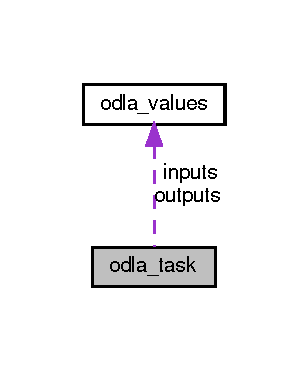
\includegraphics[width=148pt]{structodla__task__coll__graph}
\end{center}
\end{figure}
\doxysubsection*{Data Fields}
\begin{DoxyCompactItemize}
\item 
\mbox{\Hypertarget{structodla__task_abc47619ed14e6f37aad56c6b6cec3e63}\label{structodla__task_abc47619ed14e6f37aad56c6b6cec3e63}} 
void($\ast$ {\bfseries func} )(\mbox{\hyperlink{odla__device_8h_aaeace6ca8143dfbca7fbc71736b0c2ae}{odla\+\_\+device}}, \mbox{\hyperlink{structodla__values}{odla\+\_\+values}} inputs, \mbox{\hyperlink{structodla__values}{odla\+\_\+values}} outputs)
\item 
\mbox{\Hypertarget{structodla__task_a0884e3803ea11dc88a1dbea6cbec8d0c}\label{structodla__task_a0884e3803ea11dc88a1dbea6cbec8d0c}} 
\mbox{\hyperlink{structodla__values}{odla\+\_\+values}} {\bfseries inputs}
\item 
\mbox{\Hypertarget{structodla__task_aae56730d238191ca72a02cb178c25c45}\label{structodla__task_aae56730d238191ca72a02cb178c25c45}} 
\mbox{\hyperlink{structodla__values}{odla\+\_\+values}} {\bfseries outputs}
\end{DoxyCompactItemize}


\doxysubsection{Detailed Description}
odla task definition 

Definition at line 34 of file odla\+\_\+task.\+h.



The documentation for this struct was generated from the following file\+:\begin{DoxyCompactItemize}
\item 
O\+D\+L\+A/\mbox{\hyperlink{odla__task_8h}{odla\+\_\+task.\+h}}\end{DoxyCompactItemize}

\hypertarget{structodla__value__ids}{}\doxysection{odla\+\_\+value\+\_\+ids Struct Reference}
\label{structodla__value__ids}\index{odla\_value\_ids@{odla\_value\_ids}}


Multiple value ids.  


\doxysubsection*{Data Fields}
\begin{DoxyCompactItemize}
\item 
\mbox{\Hypertarget{structodla__value__ids_a501c149390cee1e8ded39313bb5ddde8}\label{structodla__value__ids_a501c149390cee1e8ded39313bb5ddde8}} 
\mbox{\hyperlink{odla__common_8h_a3579cace9c3247094d82fd2a6b09fa84}{odla\+\_\+size\+\_\+t}} {\bfseries size}
\item 
\mbox{\Hypertarget{structodla__value__ids_afe1dd6ff50cb0d266f8c81bf5c644f7a}\label{structodla__value__ids_afe1dd6ff50cb0d266f8c81bf5c644f7a}} 
\mbox{\hyperlink{odla__value_8h_a875459af53aca134ae1b1d82e971ec82}{odla\+\_\+value\+\_\+id}} {\bfseries value\+\_\+ids} \mbox{[}\mbox{\hyperlink{odla__value_8h_a7fd4a97be34945b2a2f70ddae3b30e23}{ODLA\+\_\+\+MAX\+\_\+\+OUTPUTS}}\mbox{]}
\end{DoxyCompactItemize}


\doxysubsection{Detailed Description}
Multiple value ids. 

Definition at line 64 of file odla\+\_\+value.\+h.



The documentation for this struct was generated from the following file\+:\begin{DoxyCompactItemize}
\item 
ODLA/\mbox{\hyperlink{odla__value_8h}{odla\+\_\+value.\+h}}\end{DoxyCompactItemize}

\hypertarget{structodla__value__quant__info}{}\doxysection{odla\+\_\+value\+\_\+quant\+\_\+info Struct Reference}
\label{structodla__value__quant__info}\index{odla\_value\_quant\_info@{odla\_value\_quant\_info}}


Quantization info for each odla value.  


\doxysubsection*{Data Fields}
\begin{DoxyCompactItemize}
\item 
\mbox{\Hypertarget{structodla__value__quant__info_a164cd56125ec41328d1340e992c11247}\label{structodla__value__quant__info_a164cd56125ec41328d1340e992c11247}} 
\mbox{\hyperlink{odla__value_8h_a875459af53aca134ae1b1d82e971ec82}{odla\+\_\+value\+\_\+id}} {\bfseries value\+\_\+id}
\item 
\mbox{\Hypertarget{structodla__value__quant__info_ae4ce8c1f40edf4b5a1d5ecfad66ee805}\label{structodla__value__quant__info_ae4ce8c1f40edf4b5a1d5ecfad66ee805}} 
int {\bfseries ch\+\_\+idx}
\item 
\mbox{\Hypertarget{structodla__value__quant__info_a640c56e2db43c8d17fd0c7723581c0e6}\label{structodla__value__quant__info_a640c56e2db43c8d17fd0c7723581c0e6}} 
\mbox{\hyperlink{odla__common_8h_aeaf2b4ed87e14f5bbf792ab782aa73f5}{odla\+\_\+float32}} {\bfseries scale}
\item 
\mbox{\Hypertarget{structodla__value__quant__info_a8aa9ed68a03e37795cf39ae988f9a618}\label{structodla__value__quant__info_a8aa9ed68a03e37795cf39ae988f9a618}} 
\mbox{\hyperlink{odla__common_8h_aeaf2b4ed87e14f5bbf792ab782aa73f5}{odla\+\_\+float32}} {\bfseries offset}
\item 
\mbox{\Hypertarget{structodla__value__quant__info_ab62cdf39bcb6db8b6504fa56fc5f7560}\label{structodla__value__quant__info_ab62cdf39bcb6db8b6504fa56fc5f7560}} 
\mbox{\hyperlink{odla__common_8h_aeaf2b4ed87e14f5bbf792ab782aa73f5}{odla\+\_\+float32}} {\bfseries min}
\item 
\mbox{\Hypertarget{structodla__value__quant__info_a3c6eae3feb0846f3e0fc5959363772af}\label{structodla__value__quant__info_a3c6eae3feb0846f3e0fc5959363772af}} 
\mbox{\hyperlink{odla__common_8h_aeaf2b4ed87e14f5bbf792ab782aa73f5}{odla\+\_\+float32}} {\bfseries max}
\end{DoxyCompactItemize}


\doxysubsection{Detailed Description}
Quantization info for each odla value. 

Definition at line 33 of file odla\+\_\+ops\+\_\+quantization.\+h.



The documentation for this struct was generated from the following file\+:\begin{DoxyCompactItemize}
\item 
ODLA/ops/\mbox{\hyperlink{odla__ops__quantization_8h}{odla\+\_\+ops\+\_\+quantization.\+h}}\end{DoxyCompactItemize}

\hypertarget{structodla__value__shape}{}\doxysection{odla\+\_\+value\+\_\+shape Struct Reference}
\label{structodla__value__shape}\index{odla\_value\_shape@{odla\_value\_shape}}


Shape of value.  


\doxysubsection*{Data Fields}
\begin{DoxyCompactItemize}
\item 
\mbox{\Hypertarget{structodla__value__shape_a2de1ed7d13ccf5e77eea10f404475a56}\label{structodla__value__shape_a2de1ed7d13ccf5e77eea10f404475a56}} 
\mbox{\hyperlink{odla__common_8h_a5cb8cabb738bd27c7cc6bff62aa4b19f}{odla\+\_\+int32}} {\bfseries size}
\item 
\mbox{\Hypertarget{structodla__value__shape_a33778efb57bdfa6c2bb6fa4a5a25697a}\label{structodla__value__shape_a33778efb57bdfa6c2bb6fa4a5a25697a}} 
\mbox{\hyperlink{odla__common_8h_af6306075da68e69eb72994ba9a6b3aa5}{odla\+\_\+int64}} {\bfseries dims} \mbox{[}\mbox{\hyperlink{odla__value_8h_a398ef994746c9294e4c1239f549a682f}{ODLA\+\_\+\+MAX\+\_\+\+DIMENSION}}\mbox{]}
\end{DoxyCompactItemize}


\doxysubsection{Detailed Description}
Shape of value. 

Definition at line 38 of file odla\+\_\+value.\+h.



The documentation for this struct was generated from the following file\+:\begin{DoxyCompactItemize}
\item 
ODLA/\mbox{\hyperlink{odla__value_8h}{odla\+\_\+value.\+h}}\end{DoxyCompactItemize}

\hypertarget{structodla__value__type}{}\doxysection{odla\+\_\+value\+\_\+type Struct Reference}
\label{structodla__value__type}\index{odla\_value\_type@{odla\_value\_type}}


Type of value.  




Collaboration diagram for odla\+\_\+value\+\_\+type\+:
\nopagebreak
\begin{figure}[H]
\begin{center}
\leavevmode
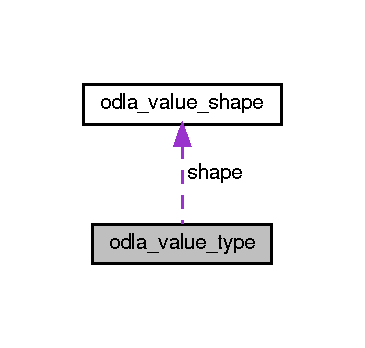
\includegraphics[width=175pt]{structodla__value__type__coll__graph}
\end{center}
\end{figure}
\doxysubsection*{Data Fields}
\begin{DoxyCompactItemize}
\item 
\mbox{\Hypertarget{structodla__value__type_a926941f930d1de2f44be7767d40e3402}\label{structodla__value__type_a926941f930d1de2f44be7767d40e3402}} 
odla\+\_\+element\+\_\+type {\bfseries element\+\_\+type}
\item 
\mbox{\Hypertarget{structodla__value__type_a71e32dec2c65553cba0d3612f9facb0d}\label{structodla__value__type_a71e32dec2c65553cba0d3612f9facb0d}} 
\mbox{\hyperlink{structodla__value__shape}{odla\+\_\+value\+\_\+shape}} {\bfseries shape}
\end{DoxyCompactItemize}


\doxysubsection{Detailed Description}
Type of value. 

Definition at line 46 of file odla\+\_\+value.\+h.



The documentation for this struct was generated from the following file\+:\begin{DoxyCompactItemize}
\item 
ODLA/\mbox{\hyperlink{odla__value_8h}{odla\+\_\+value.\+h}}\end{DoxyCompactItemize}

\hypertarget{structodla__values}{}\doxysection{odla\+\_\+values Struct Reference}
\label{structodla__values}\index{odla\_values@{odla\_values}}


Multiple values.  


\doxysubsection*{Data Fields}
\begin{DoxyCompactItemize}
\item 
\mbox{\Hypertarget{structodla__values_a6e41ada4101881ea20fea4c64ea28ac3}\label{structodla__values_a6e41ada4101881ea20fea4c64ea28ac3}} 
\mbox{\hyperlink{odla__common_8h_a3579cace9c3247094d82fd2a6b09fa84}{odla\+\_\+size\+\_\+t}} {\bfseries size}
\item 
\mbox{\Hypertarget{structodla__values_a7ce0300f9688e94931eb9b6a05f86d59}\label{structodla__values_a7ce0300f9688e94931eb9b6a05f86d59}} 
\mbox{\hyperlink{odla__value_8h_ace8591dbfa7d6ec7c38533286be8490b}{odla\+\_\+value}} {\bfseries values} \mbox{[}\mbox{\hyperlink{odla__value_8h_a7fd4a97be34945b2a2f70ddae3b30e23}{ODLA\+\_\+\+MAX\+\_\+\+OUTPUTS}}\mbox{]}
\end{DoxyCompactItemize}


\doxysubsection{Detailed Description}
Multiple values. 

Definition at line 55 of file odla\+\_\+value.\+h.



The documentation for this struct was generated from the following file\+:\begin{DoxyCompactItemize}
\item 
ODLA/\mbox{\hyperlink{odla__value_8h}{odla\+\_\+value.\+h}}\end{DoxyCompactItemize}

\chapter{File Documentation}
\hypertarget{odla_8h}{}\doxysection{O\+D\+L\+A/odla.h File Reference}
\label{odla_8h}\index{ODLA/odla.h@{ODLA/odla.h}}


\doxysubsection{Detailed Description}
This file defines the O\+D\+LA entry point. 
\hypertarget{odla__common_8h}{}\doxysection{O\+D\+L\+A/odla\+\_\+common.h File Reference}
\label{odla__common_8h}\index{ODLA/odla\_common.h@{ODLA/odla\_common.h}}
\doxysubsection*{Macros}
\begin{DoxyCompactItemize}
\item 
\mbox{\Hypertarget{odla__common_8h_a1f9123e77ab174e483a7f307eb9c264e}\label{odla__common_8h_a1f9123e77ab174e483a7f307eb9c264e}} 
\#define \mbox{\hyperlink{odla__common_8h_a1f9123e77ab174e483a7f307eb9c264e}{O\+D\+L\+A\+\_\+\+A\+P\+I\+\_\+\+E\+X\+P\+O\+RT}}
\begin{DoxyCompactList}\small\item\em A\+PI export directives. \end{DoxyCompactList}\item 
\mbox{\Hypertarget{odla__common_8h_a115004e03b7bafa9bd7ab433afc7ac5f}\label{odla__common_8h_a115004e03b7bafa9bd7ab433afc7ac5f}} 
\#define {\bfseries O\+D\+L\+A\+\_\+\+A\+P\+I\+\_\+\+C\+A\+LL}
\end{DoxyCompactItemize}
\doxysubsection*{Typedefs}
\begin{DoxyCompactItemize}
\item 
typedef int8\+\_\+t \mbox{\hyperlink{odla__common_8h_af5b2e32e5c9dcb9a840946c975fae7c6}{odla\+\_\+int8}}
\item 
typedef int16\+\_\+t \mbox{\hyperlink{odla__common_8h_a5f828748cf25e29702f9e8a3f59cb51d}{odla\+\_\+int16}}
\item 
typedef int32\+\_\+t \mbox{\hyperlink{odla__common_8h_a5cb8cabb738bd27c7cc6bff62aa4b19f}{odla\+\_\+int32}}
\item 
typedef int64\+\_\+t \mbox{\hyperlink{odla__common_8h_af6306075da68e69eb72994ba9a6b3aa5}{odla\+\_\+int64}}
\item 
typedef uint8\+\_\+t \mbox{\hyperlink{odla__common_8h_a1a9fda9a9a616a3b6327f60f18b23ebd}{odla\+\_\+uint8}}
\item 
typedef uint16\+\_\+t \mbox{\hyperlink{odla__common_8h_a643350f4b28f34b4eb7131f9e106368d}{odla\+\_\+uint16}}
\item 
typedef uint32\+\_\+t \mbox{\hyperlink{odla__common_8h_a909bbb71e3a1f9ef49083a8256465c9c}{odla\+\_\+uint32}}
\item 
typedef uint64\+\_\+t \mbox{\hyperlink{odla__common_8h_a624e95ec2972c9f5d3f770e98b40c1e1}{odla\+\_\+uint64}}
\item 
typedef int8\+\_\+t \mbox{\hyperlink{odla__common_8h_a351e3c5bb2dac055c077354e7a4feb49}{odla\+\_\+qint8}}
\item 
typedef int16\+\_\+t \mbox{\hyperlink{odla__common_8h_ab058e0743da06e65c065ea97dbd2b1ce}{odla\+\_\+qint16}}
\item 
typedef int32\+\_\+t \mbox{\hyperlink{odla__common_8h_a01b2ae6b2aec31f8d04e19879d81be7a}{odla\+\_\+qint32}}
\item 
typedef int64\+\_\+t \mbox{\hyperlink{odla__common_8h_a3e0729965e00db9ec8565878a2cbfff4}{odla\+\_\+qint64}}
\item 
typedef uint8\+\_\+t \mbox{\hyperlink{odla__common_8h_aaff55ff3e4355c7b0fed47e0d3607975}{odla\+\_\+quint8}}
\item 
typedef uint16\+\_\+t \mbox{\hyperlink{odla__common_8h_a2cb5bfde7e306955a15abf6a040b86aa}{odla\+\_\+quint16}}
\item 
typedef uint32\+\_\+t \mbox{\hyperlink{odla__common_8h_a340a99b7098b8f4d98d5e328ff632604}{odla\+\_\+quint32}}
\item 
typedef uint64\+\_\+t \mbox{\hyperlink{odla__common_8h_a6fdb6723b3e91a5e56c7d5cdf1b31597}{odla\+\_\+quint64}}
\item 
typedef uint16\+\_\+t \mbox{\hyperlink{odla__common_8h_af471ef78542a9702c2782dacaba252cd}{odla\+\_\+float16}}
\item 
typedef uint16\+\_\+t \mbox{\hyperlink{odla__common_8h_a27c4357b8c5162df40fd1e5b03b45d06}{odla\+\_\+bfloat16}}
\item 
typedef float \mbox{\hyperlink{odla__common_8h_aeaf2b4ed87e14f5bbf792ab782aa73f5}{odla\+\_\+float32}}
\item 
typedef double \mbox{\hyperlink{odla__common_8h_a956bdf1765e13ccacb04cbf02de7d0b3}{odla\+\_\+float64}}
\item 
typedef \mbox{\hyperlink{odla__common_8h_a909bbb71e3a1f9ef49083a8256465c9c}{odla\+\_\+uint32}} \mbox{\hyperlink{odla__common_8h_a86f265601c0773152f4e193a8614c0ac}{odla\+\_\+bool}}
\item 
\mbox{\Hypertarget{odla__common_8h_a70ab5c97f8e2150ab1c252e6fa33d38b}\label{odla__common_8h_a70ab5c97f8e2150ab1c252e6fa33d38b}} 
typedef char \mbox{\hyperlink{odla__common_8h_a70ab5c97f8e2150ab1c252e6fa33d38b}{odla\+\_\+char}}
\begin{DoxyCompactList}\small\item\em char \end{DoxyCompactList}\item 
\mbox{\Hypertarget{odla__common_8h_a3579cace9c3247094d82fd2a6b09fa84}\label{odla__common_8h_a3579cace9c3247094d82fd2a6b09fa84}} 
typedef size\+\_\+t \mbox{\hyperlink{odla__common_8h_a3579cace9c3247094d82fd2a6b09fa84}{odla\+\_\+size\+\_\+t}}
\begin{DoxyCompactList}\small\item\em size\+\_\+t \end{DoxyCompactList}\item 
\mbox{\Hypertarget{odla__common_8h_ada3e0e93ebd03f1f5fe3ff21655cdb11}\label{odla__common_8h_ada3e0e93ebd03f1f5fe3ff21655cdb11}} 
typedef void \mbox{\hyperlink{odla__common_8h_ada3e0e93ebd03f1f5fe3ff21655cdb11}{odla\+\_\+void}}
\begin{DoxyCompactList}\small\item\em void \end{DoxyCompactList}\end{DoxyCompactItemize}
\doxysubsection*{Enumerations}
\begin{DoxyCompactItemize}
\item 
\mbox{\Hypertarget{odla__common_8h_a6218e6a4a89e7525ee0506df9bf2d934}\label{odla__common_8h_a6218e6a4a89e7525ee0506df9bf2d934}} 
enum {\bfseries odla\+\_\+element\+\_\+type} \{ \newline
{\bfseries O\+D\+L\+A\+\_\+\+I\+N\+T8}, 
{\bfseries O\+D\+L\+A\+\_\+\+I\+N\+T16}, 
{\bfseries O\+D\+L\+A\+\_\+\+I\+N\+T32}, 
{\bfseries O\+D\+L\+A\+\_\+\+I\+N\+T64}, 
\newline
{\bfseries O\+D\+L\+A\+\_\+\+U\+I\+N\+T8}, 
{\bfseries O\+D\+L\+A\+\_\+\+U\+I\+N\+T16}, 
{\bfseries O\+D\+L\+A\+\_\+\+U\+I\+N\+T32}, 
{\bfseries O\+D\+L\+A\+\_\+\+U\+I\+N\+T64}, 
\newline
{\bfseries O\+D\+L\+A\+\_\+\+Q\+I\+N\+T8}, 
{\bfseries O\+D\+L\+A\+\_\+\+Q\+I\+N\+T16}, 
{\bfseries O\+D\+L\+A\+\_\+\+Q\+I\+N\+T32}, 
{\bfseries O\+D\+L\+A\+\_\+\+Q\+I\+N\+T64}, 
\newline
{\bfseries O\+D\+L\+A\+\_\+\+Q\+U\+I\+N\+T8}, 
{\bfseries O\+D\+L\+A\+\_\+\+Q\+U\+I\+N\+T16}, 
{\bfseries O\+D\+L\+A\+\_\+\+Q\+U\+I\+N\+T32}, 
{\bfseries O\+D\+L\+A\+\_\+\+Q\+U\+I\+N\+T64}, 
\newline
{\bfseries O\+D\+L\+A\+\_\+\+F\+L\+O\+A\+T16}, 
{\bfseries O\+D\+L\+A\+\_\+\+B\+F\+L\+O\+A\+T16}, 
{\bfseries O\+D\+L\+A\+\_\+\+F\+L\+O\+A\+T32}, 
{\bfseries O\+D\+L\+A\+\_\+\+F\+L\+O\+A\+T64}, 
\newline
{\bfseries O\+D\+L\+A\+\_\+\+B\+O\+OL}
 \}
\item 
\mbox{\Hypertarget{odla__common_8h_a32d12bc3360c8b8891c225a703f7db29}\label{odla__common_8h_a32d12bc3360c8b8891c225a703f7db29}} 
enum \mbox{\hyperlink{odla__common_8h_a32d12bc3360c8b8891c225a703f7db29}{odla\+\_\+status}} \{ {\bfseries O\+D\+L\+A\+\_\+\+S\+U\+C\+C\+E\+SS}, 
{\bfseries O\+D\+L\+A\+\_\+\+F\+A\+I\+L\+U\+RE}
 \}
\begin{DoxyCompactList}\small\item\em Return status. \end{DoxyCompactList}\end{DoxyCompactItemize}


\doxysubsection{Detailed Description}
This file defines the O\+D\+LA basic common types. 

\doxysubsection{Typedef Documentation}
\mbox{\Hypertarget{odla__common_8h_a27c4357b8c5162df40fd1e5b03b45d06}\label{odla__common_8h_a27c4357b8c5162df40fd1e5b03b45d06}} 
\index{odla\_common.h@{odla\_common.h}!odla\_bfloat16@{odla\_bfloat16}}
\index{odla\_bfloat16@{odla\_bfloat16}!odla\_common.h@{odla\_common.h}}
\doxysubsubsection{\texorpdfstring{odla\_bfloat16}{odla\_bfloat16}}
{\footnotesize\ttfamily typedef uint16\+\_\+t \mbox{\hyperlink{odla__common_8h_a27c4357b8c5162df40fd1e5b03b45d06}{odla\+\_\+bfloat16}}}

16-\/bit brain floating point type 

Definition at line 87 of file odla\+\_\+common.\+h.

\mbox{\Hypertarget{odla__common_8h_a86f265601c0773152f4e193a8614c0ac}\label{odla__common_8h_a86f265601c0773152f4e193a8614c0ac}} 
\index{odla\_common.h@{odla\_common.h}!odla\_bool@{odla\_bool}}
\index{odla\_bool@{odla\_bool}!odla\_common.h@{odla\_common.h}}
\doxysubsubsection{\texorpdfstring{odla\_bool}{odla\_bool}}
{\footnotesize\ttfamily typedef \mbox{\hyperlink{odla__common_8h_a909bbb71e3a1f9ef49083a8256465c9c}{odla\+\_\+uint32}} \mbox{\hyperlink{odla__common_8h_a86f265601c0773152f4e193a8614c0ac}{odla\+\_\+bool}}}

boolean type 

Definition at line 92 of file odla\+\_\+common.\+h.

\mbox{\Hypertarget{odla__common_8h_af471ef78542a9702c2782dacaba252cd}\label{odla__common_8h_af471ef78542a9702c2782dacaba252cd}} 
\index{odla\_common.h@{odla\_common.h}!odla\_float16@{odla\_float16}}
\index{odla\_float16@{odla\_float16}!odla\_common.h@{odla\_common.h}}
\doxysubsubsection{\texorpdfstring{odla\_float16}{odla\_float16}}
{\footnotesize\ttfamily typedef uint16\+\_\+t \mbox{\hyperlink{odla__common_8h_af471ef78542a9702c2782dacaba252cd}{odla\+\_\+float16}}}

16-\/bit floating point type 

Definition at line 86 of file odla\+\_\+common.\+h.

\mbox{\Hypertarget{odla__common_8h_aeaf2b4ed87e14f5bbf792ab782aa73f5}\label{odla__common_8h_aeaf2b4ed87e14f5bbf792ab782aa73f5}} 
\index{odla\_common.h@{odla\_common.h}!odla\_float32@{odla\_float32}}
\index{odla\_float32@{odla\_float32}!odla\_common.h@{odla\_common.h}}
\doxysubsubsection{\texorpdfstring{odla\_float32}{odla\_float32}}
{\footnotesize\ttfamily typedef float \mbox{\hyperlink{odla__common_8h_aeaf2b4ed87e14f5bbf792ab782aa73f5}{odla\+\_\+float32}}}

32-\/bit floating point type 

Definition at line 88 of file odla\+\_\+common.\+h.

\mbox{\Hypertarget{odla__common_8h_a956bdf1765e13ccacb04cbf02de7d0b3}\label{odla__common_8h_a956bdf1765e13ccacb04cbf02de7d0b3}} 
\index{odla\_common.h@{odla\_common.h}!odla\_float64@{odla\_float64}}
\index{odla\_float64@{odla\_float64}!odla\_common.h@{odla\_common.h}}
\doxysubsubsection{\texorpdfstring{odla\_float64}{odla\_float64}}
{\footnotesize\ttfamily typedef double \mbox{\hyperlink{odla__common_8h_a956bdf1765e13ccacb04cbf02de7d0b3}{odla\+\_\+float64}}}

64-\/bit floating point type 

Definition at line 89 of file odla\+\_\+common.\+h.

\mbox{\Hypertarget{odla__common_8h_a5f828748cf25e29702f9e8a3f59cb51d}\label{odla__common_8h_a5f828748cf25e29702f9e8a3f59cb51d}} 
\index{odla\_common.h@{odla\_common.h}!odla\_int16@{odla\_int16}}
\index{odla\_int16@{odla\_int16}!odla\_common.h@{odla\_common.h}}
\doxysubsubsection{\texorpdfstring{odla\_int16}{odla\_int16}}
{\footnotesize\ttfamily typedef int16\+\_\+t \mbox{\hyperlink{odla__common_8h_a5f828748cf25e29702f9e8a3f59cb51d}{odla\+\_\+int16}}}

16-\/bit signed integer type 

Definition at line 67 of file odla\+\_\+common.\+h.

\mbox{\Hypertarget{odla__common_8h_a5cb8cabb738bd27c7cc6bff62aa4b19f}\label{odla__common_8h_a5cb8cabb738bd27c7cc6bff62aa4b19f}} 
\index{odla\_common.h@{odla\_common.h}!odla\_int32@{odla\_int32}}
\index{odla\_int32@{odla\_int32}!odla\_common.h@{odla\_common.h}}
\doxysubsubsection{\texorpdfstring{odla\_int32}{odla\_int32}}
{\footnotesize\ttfamily typedef int32\+\_\+t \mbox{\hyperlink{odla__common_8h_a5cb8cabb738bd27c7cc6bff62aa4b19f}{odla\+\_\+int32}}}

32-\/bit signed integer type 

Definition at line 68 of file odla\+\_\+common.\+h.

\mbox{\Hypertarget{odla__common_8h_af6306075da68e69eb72994ba9a6b3aa5}\label{odla__common_8h_af6306075da68e69eb72994ba9a6b3aa5}} 
\index{odla\_common.h@{odla\_common.h}!odla\_int64@{odla\_int64}}
\index{odla\_int64@{odla\_int64}!odla\_common.h@{odla\_common.h}}
\doxysubsubsection{\texorpdfstring{odla\_int64}{odla\_int64}}
{\footnotesize\ttfamily typedef int64\+\_\+t \mbox{\hyperlink{odla__common_8h_af6306075da68e69eb72994ba9a6b3aa5}{odla\+\_\+int64}}}

64-\/bit signed integer type 

Definition at line 69 of file odla\+\_\+common.\+h.

\mbox{\Hypertarget{odla__common_8h_af5b2e32e5c9dcb9a840946c975fae7c6}\label{odla__common_8h_af5b2e32e5c9dcb9a840946c975fae7c6}} 
\index{odla\_common.h@{odla\_common.h}!odla\_int8@{odla\_int8}}
\index{odla\_int8@{odla\_int8}!odla\_common.h@{odla\_common.h}}
\doxysubsubsection{\texorpdfstring{odla\_int8}{odla\_int8}}
{\footnotesize\ttfamily typedef int8\+\_\+t \mbox{\hyperlink{odla__common_8h_af5b2e32e5c9dcb9a840946c975fae7c6}{odla\+\_\+int8}}}

8-\/bit signed integer type 

Definition at line 66 of file odla\+\_\+common.\+h.

\mbox{\Hypertarget{odla__common_8h_ab058e0743da06e65c065ea97dbd2b1ce}\label{odla__common_8h_ab058e0743da06e65c065ea97dbd2b1ce}} 
\index{odla\_common.h@{odla\_common.h}!odla\_qint16@{odla\_qint16}}
\index{odla\_qint16@{odla\_qint16}!odla\_common.h@{odla\_common.h}}
\doxysubsubsection{\texorpdfstring{odla\_qint16}{odla\_qint16}}
{\footnotesize\ttfamily typedef int16\+\_\+t \mbox{\hyperlink{odla__common_8h_ab058e0743da06e65c065ea97dbd2b1ce}{odla\+\_\+qint16}}}

16-\/bit signed quantized integer type 

Definition at line 77 of file odla\+\_\+common.\+h.

\mbox{\Hypertarget{odla__common_8h_a01b2ae6b2aec31f8d04e19879d81be7a}\label{odla__common_8h_a01b2ae6b2aec31f8d04e19879d81be7a}} 
\index{odla\_common.h@{odla\_common.h}!odla\_qint32@{odla\_qint32}}
\index{odla\_qint32@{odla\_qint32}!odla\_common.h@{odla\_common.h}}
\doxysubsubsection{\texorpdfstring{odla\_qint32}{odla\_qint32}}
{\footnotesize\ttfamily typedef int32\+\_\+t \mbox{\hyperlink{odla__common_8h_a01b2ae6b2aec31f8d04e19879d81be7a}{odla\+\_\+qint32}}}

32-\/bit signed quantized integer type 

Definition at line 78 of file odla\+\_\+common.\+h.

\mbox{\Hypertarget{odla__common_8h_a3e0729965e00db9ec8565878a2cbfff4}\label{odla__common_8h_a3e0729965e00db9ec8565878a2cbfff4}} 
\index{odla\_common.h@{odla\_common.h}!odla\_qint64@{odla\_qint64}}
\index{odla\_qint64@{odla\_qint64}!odla\_common.h@{odla\_common.h}}
\doxysubsubsection{\texorpdfstring{odla\_qint64}{odla\_qint64}}
{\footnotesize\ttfamily typedef int64\+\_\+t \mbox{\hyperlink{odla__common_8h_a3e0729965e00db9ec8565878a2cbfff4}{odla\+\_\+qint64}}}

64-\/bit signed quantized integer type 

Definition at line 79 of file odla\+\_\+common.\+h.

\mbox{\Hypertarget{odla__common_8h_a351e3c5bb2dac055c077354e7a4feb49}\label{odla__common_8h_a351e3c5bb2dac055c077354e7a4feb49}} 
\index{odla\_common.h@{odla\_common.h}!odla\_qint8@{odla\_qint8}}
\index{odla\_qint8@{odla\_qint8}!odla\_common.h@{odla\_common.h}}
\doxysubsubsection{\texorpdfstring{odla\_qint8}{odla\_qint8}}
{\footnotesize\ttfamily typedef int8\+\_\+t \mbox{\hyperlink{odla__common_8h_a351e3c5bb2dac055c077354e7a4feb49}{odla\+\_\+qint8}}}

8-\/bit signed quantized integer type 

Definition at line 76 of file odla\+\_\+common.\+h.

\mbox{\Hypertarget{odla__common_8h_a2cb5bfde7e306955a15abf6a040b86aa}\label{odla__common_8h_a2cb5bfde7e306955a15abf6a040b86aa}} 
\index{odla\_common.h@{odla\_common.h}!odla\_quint16@{odla\_quint16}}
\index{odla\_quint16@{odla\_quint16}!odla\_common.h@{odla\_common.h}}
\doxysubsubsection{\texorpdfstring{odla\_quint16}{odla\_quint16}}
{\footnotesize\ttfamily typedef uint16\+\_\+t \mbox{\hyperlink{odla__common_8h_a2cb5bfde7e306955a15abf6a040b86aa}{odla\+\_\+quint16}}}

16-\/bit unsigned quantized integer type 

Definition at line 81 of file odla\+\_\+common.\+h.

\mbox{\Hypertarget{odla__common_8h_a340a99b7098b8f4d98d5e328ff632604}\label{odla__common_8h_a340a99b7098b8f4d98d5e328ff632604}} 
\index{odla\_common.h@{odla\_common.h}!odla\_quint32@{odla\_quint32}}
\index{odla\_quint32@{odla\_quint32}!odla\_common.h@{odla\_common.h}}
\doxysubsubsection{\texorpdfstring{odla\_quint32}{odla\_quint32}}
{\footnotesize\ttfamily typedef uint32\+\_\+t \mbox{\hyperlink{odla__common_8h_a340a99b7098b8f4d98d5e328ff632604}{odla\+\_\+quint32}}}

32-\/bit unsigned quantized integer type 

Definition at line 82 of file odla\+\_\+common.\+h.

\mbox{\Hypertarget{odla__common_8h_a6fdb6723b3e91a5e56c7d5cdf1b31597}\label{odla__common_8h_a6fdb6723b3e91a5e56c7d5cdf1b31597}} 
\index{odla\_common.h@{odla\_common.h}!odla\_quint64@{odla\_quint64}}
\index{odla\_quint64@{odla\_quint64}!odla\_common.h@{odla\_common.h}}
\doxysubsubsection{\texorpdfstring{odla\_quint64}{odla\_quint64}}
{\footnotesize\ttfamily typedef uint64\+\_\+t \mbox{\hyperlink{odla__common_8h_a6fdb6723b3e91a5e56c7d5cdf1b31597}{odla\+\_\+quint64}}}

64-\/bit unsigned quantized integer type 

Definition at line 83 of file odla\+\_\+common.\+h.

\mbox{\Hypertarget{odla__common_8h_aaff55ff3e4355c7b0fed47e0d3607975}\label{odla__common_8h_aaff55ff3e4355c7b0fed47e0d3607975}} 
\index{odla\_common.h@{odla\_common.h}!odla\_quint8@{odla\_quint8}}
\index{odla\_quint8@{odla\_quint8}!odla\_common.h@{odla\_common.h}}
\doxysubsubsection{\texorpdfstring{odla\_quint8}{odla\_quint8}}
{\footnotesize\ttfamily typedef uint8\+\_\+t \mbox{\hyperlink{odla__common_8h_aaff55ff3e4355c7b0fed47e0d3607975}{odla\+\_\+quint8}}}

8-\/bit unsigned quantized integer type 

Definition at line 80 of file odla\+\_\+common.\+h.

\mbox{\Hypertarget{odla__common_8h_a643350f4b28f34b4eb7131f9e106368d}\label{odla__common_8h_a643350f4b28f34b4eb7131f9e106368d}} 
\index{odla\_common.h@{odla\_common.h}!odla\_uint16@{odla\_uint16}}
\index{odla\_uint16@{odla\_uint16}!odla\_common.h@{odla\_common.h}}
\doxysubsubsection{\texorpdfstring{odla\_uint16}{odla\_uint16}}
{\footnotesize\ttfamily typedef uint16\+\_\+t \mbox{\hyperlink{odla__common_8h_a643350f4b28f34b4eb7131f9e106368d}{odla\+\_\+uint16}}}

16-\/bit unsigned integer type 

Definition at line 71 of file odla\+\_\+common.\+h.

\mbox{\Hypertarget{odla__common_8h_a909bbb71e3a1f9ef49083a8256465c9c}\label{odla__common_8h_a909bbb71e3a1f9ef49083a8256465c9c}} 
\index{odla\_common.h@{odla\_common.h}!odla\_uint32@{odla\_uint32}}
\index{odla\_uint32@{odla\_uint32}!odla\_common.h@{odla\_common.h}}
\doxysubsubsection{\texorpdfstring{odla\_uint32}{odla\_uint32}}
{\footnotesize\ttfamily typedef uint32\+\_\+t \mbox{\hyperlink{odla__common_8h_a909bbb71e3a1f9ef49083a8256465c9c}{odla\+\_\+uint32}}}

32-\/bit unsigned integer type 

Definition at line 72 of file odla\+\_\+common.\+h.

\mbox{\Hypertarget{odla__common_8h_a624e95ec2972c9f5d3f770e98b40c1e1}\label{odla__common_8h_a624e95ec2972c9f5d3f770e98b40c1e1}} 
\index{odla\_common.h@{odla\_common.h}!odla\_uint64@{odla\_uint64}}
\index{odla\_uint64@{odla\_uint64}!odla\_common.h@{odla\_common.h}}
\doxysubsubsection{\texorpdfstring{odla\_uint64}{odla\_uint64}}
{\footnotesize\ttfamily typedef uint64\+\_\+t \mbox{\hyperlink{odla__common_8h_a624e95ec2972c9f5d3f770e98b40c1e1}{odla\+\_\+uint64}}}

64-\/bit unsigned integer type 

Definition at line 73 of file odla\+\_\+common.\+h.

\mbox{\Hypertarget{odla__common_8h_a1a9fda9a9a616a3b6327f60f18b23ebd}\label{odla__common_8h_a1a9fda9a9a616a3b6327f60f18b23ebd}} 
\index{odla\_common.h@{odla\_common.h}!odla\_uint8@{odla\_uint8}}
\index{odla\_uint8@{odla\_uint8}!odla\_common.h@{odla\_common.h}}
\doxysubsubsection{\texorpdfstring{odla\_uint8}{odla\_uint8}}
{\footnotesize\ttfamily typedef uint8\+\_\+t \mbox{\hyperlink{odla__common_8h_a1a9fda9a9a616a3b6327f60f18b23ebd}{odla\+\_\+uint8}}}

8-\/bit unsigned integer type 

Definition at line 70 of file odla\+\_\+common.\+h.


\hypertarget{odla__compute_8h}{}\doxysection{ODLA/odla\+\_\+compute.h File Reference}
\label{odla__compute_8h}\index{ODLA/odla\_compute.h@{ODLA/odla\_compute.h}}
\doxysubsection*{Typedefs}
\begin{DoxyCompactItemize}
\item 
\mbox{\Hypertarget{odla__compute_8h_a7906dc5bd415fd126df428a44cfc660e}\label{odla__compute_8h_a7906dc5bd415fd126df428a44cfc660e}} 
typedef struct \+\_\+odla\+\_\+computation $\ast$ \mbox{\hyperlink{odla__compute_8h_a7906dc5bd415fd126df428a44cfc660e}{odla\+\_\+computation}}
\begin{DoxyCompactList}\small\item\em Computation object. \end{DoxyCompactList}\item 
\mbox{\Hypertarget{odla__compute_8h_a58a9f95845de8c2dcee9df9efd983aaf}\label{odla__compute_8h_a58a9f95845de8c2dcee9df9efd983aaf}} 
typedef struct \+\_\+odla\+\_\+executable $\ast$ \mbox{\hyperlink{odla__compute_8h_a58a9f95845de8c2dcee9df9efd983aaf}{odla\+\_\+executable}}
\begin{DoxyCompactList}\small\item\em Executable object. \end{DoxyCompactList}\item 
\mbox{\Hypertarget{odla__compute_8h_a6ee1db476eaea6347d96e1e0ab7e0ad7}\label{odla__compute_8h_a6ee1db476eaea6347d96e1e0ab7e0ad7}} 
typedef struct \+\_\+odla\+\_\+context $\ast$ \mbox{\hyperlink{odla__compute_8h_a6ee1db476eaea6347d96e1e0ab7e0ad7}{odla\+\_\+context}}
\begin{DoxyCompactList}\small\item\em Context object. \end{DoxyCompactList}\item 
\mbox{\Hypertarget{odla__compute_8h_ad4d602ac28a58bbb9e4bd8bb8ea704b2}\label{odla__compute_8h_ad4d602ac28a58bbb9e4bd8bb8ea704b2}} 
typedef struct \+\_\+odla\+\_\+item\+\_\+value $\ast$ \mbox{\hyperlink{odla__compute_8h_ad4d602ac28a58bbb9e4bd8bb8ea704b2}{odla\+\_\+item\+\_\+value}}
\begin{DoxyCompactList}\small\item\em Property item value object. \end{DoxyCompactList}\item 
\mbox{\Hypertarget{odla__compute_8h_aec5edf954a98e250d6c1744f4e5ba672}\label{odla__compute_8h_aec5edf954a98e250d6c1744f4e5ba672}} 
typedef struct \+\_\+odla\+\_\+constants\+\_\+array $\ast$ \mbox{\hyperlink{odla__compute_8h_aec5edf954a98e250d6c1744f4e5ba672}{odla\+\_\+constants\+\_\+array}}
\begin{DoxyCompactList}\small\item\em Constants array object. \end{DoxyCompactList}\end{DoxyCompactItemize}
\doxysubsection*{Enumerations}
\begin{DoxyCompactItemize}
\item 
\mbox{\Hypertarget{odla__compute_8h_a5cf465369118fbb3edf6d76f28616517}\label{odla__compute_8h_a5cf465369118fbb3edf6d76f28616517}} 
enum \mbox{\hyperlink{odla__compute_8h_a5cf465369118fbb3edf6d76f28616517}{odla\+\_\+compute\+\_\+mode}} \{ {\bfseries ODLA\+\_\+\+COMPUTE\+\_\+\+DEFAULT}
, {\bfseries ODLA\+\_\+\+COMPUTE\+\_\+\+INFERENCE}
, {\bfseries ODLA\+\_\+\+COMPUTE\+\_\+\+TRAINING}
 \}
\begin{DoxyCompactList}\small\item\em Compute mode. \end{DoxyCompactList}\item 
\mbox{\Hypertarget{odla__compute_8h_a6be789aa7177278446e347afcfb9aa0b}\label{odla__compute_8h_a6be789aa7177278446e347afcfb9aa0b}} 
enum \mbox{\hyperlink{odla__compute_8h_a6be789aa7177278446e347afcfb9aa0b}{odla\+\_\+item\+\_\+type}} \{ \newline
{\bfseries ODLA\+\_\+\+DYNAMIC\+\_\+\+BATCH}
, {\bfseries ODLA\+\_\+\+MIN\+\_\+\+BATCH\+\_\+\+SIZE}
, {\bfseries ODLA\+\_\+\+MAX\+\_\+\+BATCH\+\_\+\+SIZE}
, {\bfseries ODLA\+\_\+\+OPT\+\_\+\+BATCH\+\_\+\+SIZE}
, \newline
{\bfseries ODLA\+\_\+\+RUN\+\_\+\+BATCH\+\_\+\+SIZE}
, {\bfseries ODLA\+\_\+\+FP16\+\_\+\+MODE}
, {\bfseries ODLA\+\_\+\+USE\+\_\+\+SIM\+\_\+\+MODE}
, {\bfseries ODLA\+\_\+\+PROCESSOR\+\_\+\+NUM}
, \newline
{\bfseries ODLA\+\_\+\+BATCHES\+\_\+\+PER\+\_\+\+STEP}
, {\bfseries ODLA\+\_\+\+USE\+\_\+\+DATA\+\_\+\+TYPE}
 \}
\begin{DoxyCompactList}\small\item\em Property item type. \end{DoxyCompactList}\end{DoxyCompactItemize}
\doxysubsection*{Functions}
\begin{DoxyCompactItemize}
\item 
\mbox{\hyperlink{odla__common_8h_a1f9123e77ab174e483a7f307eb9c264e}{ODLA\+\_\+\+API\+\_\+\+EXPORT}} \mbox{\hyperlink{odla__common_8h_a32d12bc3360c8b8891c225a703f7db29}{odla\+\_\+status}} ODLA\+\_\+\+API\+\_\+\+CALL \mbox{\hyperlink{odla__compute_8h_aedc3cc00aac00f6ea608c4968fc76178}{odla\+\_\+\+Create\+Computation}} (\mbox{\hyperlink{odla__compute_8h_a7906dc5bd415fd126df428a44cfc660e}{odla\+\_\+computation}} $\ast$computation)
\begin{DoxyCompactList}\small\item\em Create a computation object. \end{DoxyCompactList}\item 
\mbox{\hyperlink{odla__common_8h_a1f9123e77ab174e483a7f307eb9c264e}{ODLA\+\_\+\+API\+\_\+\+EXPORT}} \mbox{\hyperlink{odla__common_8h_a32d12bc3360c8b8891c225a703f7db29}{odla\+\_\+status}} ODLA\+\_\+\+API\+\_\+\+CALL \mbox{\hyperlink{odla__compute_8h_ae3bf1987e563cd2755890db9497a59a8}{odla\+\_\+\+Compile\+Computation}} (const \mbox{\hyperlink{odla__compute_8h_a7906dc5bd415fd126df428a44cfc660e}{odla\+\_\+computation}} computation, \mbox{\hyperlink{odla__compute_8h_a58a9f95845de8c2dcee9df9efd983aaf}{odla\+\_\+executable}} $\ast$executable)
\begin{DoxyCompactList}\small\item\em Compile a computation object into executable. \end{DoxyCompactList}\item 
\mbox{\hyperlink{odla__common_8h_a1f9123e77ab174e483a7f307eb9c264e}{ODLA\+\_\+\+API\+\_\+\+EXPORT}} \mbox{\hyperlink{odla__common_8h_a32d12bc3360c8b8891c225a703f7db29}{odla\+\_\+status}} ODLA\+\_\+\+API\+\_\+\+CALL \mbox{\hyperlink{odla__compute_8h_aa86e465d71ac084cf74b006d1437c59b}{odla\+\_\+\+Load\+Computation}} (const \mbox{\hyperlink{odla__common_8h_a70ab5c97f8e2150ab1c252e6fa33d38b}{odla\+\_\+char}} $\ast$file\+\_\+name, \mbox{\hyperlink{odla__compute_8h_a7906dc5bd415fd126df428a44cfc660e}{odla\+\_\+computation}} $\ast$computation)
\begin{DoxyCompactList}\small\item\em Load a computation from the file system. \end{DoxyCompactList}\item 
\mbox{\hyperlink{odla__common_8h_a1f9123e77ab174e483a7f307eb9c264e}{ODLA\+\_\+\+API\+\_\+\+EXPORT}} \mbox{\hyperlink{odla__common_8h_a32d12bc3360c8b8891c225a703f7db29}{odla\+\_\+status}} ODLA\+\_\+\+API\+\_\+\+CALL \mbox{\hyperlink{odla__compute_8h_a0b551a95a03962d03b6cd8d18b400ac4}{odla\+\_\+\+Store\+Computation}} (const \mbox{\hyperlink{odla__common_8h_a70ab5c97f8e2150ab1c252e6fa33d38b}{odla\+\_\+char}} $\ast$file\+\_\+name, const \mbox{\hyperlink{odla__compute_8h_a7906dc5bd415fd126df428a44cfc660e}{odla\+\_\+computation}} computation)
\begin{DoxyCompactList}\small\item\em Store a computation object into the file system. \end{DoxyCompactList}\item 
\mbox{\hyperlink{odla__common_8h_a1f9123e77ab174e483a7f307eb9c264e}{ODLA\+\_\+\+API\+\_\+\+EXPORT}} \mbox{\hyperlink{odla__common_8h_a32d12bc3360c8b8891c225a703f7db29}{odla\+\_\+status}} ODLA\+\_\+\+API\+\_\+\+CALL \mbox{\hyperlink{odla__compute_8h_a2d42e143efcda54765a4ed1b3b0c9986}{odla\+\_\+\+Differentiate\+Computation}} (\mbox{\hyperlink{odla__compute_8h_a7906dc5bd415fd126df428a44cfc660e}{odla\+\_\+computation}} computation)
\begin{DoxyCompactList}\small\item\em Differentiate a computation. \end{DoxyCompactList}\item 
\mbox{\hyperlink{odla__common_8h_a1f9123e77ab174e483a7f307eb9c264e}{ODLA\+\_\+\+API\+\_\+\+EXPORT}} \mbox{\hyperlink{odla__common_8h_a32d12bc3360c8b8891c225a703f7db29}{odla\+\_\+status}} ODLA\+\_\+\+API\+\_\+\+CALL \mbox{\hyperlink{odla__compute_8h_aa164c55ee48284ef1dc9766deeaa38c2}{odla\+\_\+\+Execute\+Computation}} (const \mbox{\hyperlink{odla__compute_8h_a7906dc5bd415fd126df428a44cfc660e}{odla\+\_\+computation}} computation, const \mbox{\hyperlink{odla__compute_8h_a6ee1db476eaea6347d96e1e0ab7e0ad7}{odla\+\_\+context}} context, const \mbox{\hyperlink{odla__compute_8h_a5cf465369118fbb3edf6d76f28616517}{odla\+\_\+compute\+\_\+mode}} mode, \mbox{\hyperlink{odla__device_8h_aaeace6ca8143dfbca7fbc71736b0c2ae}{odla\+\_\+device}} device)
\begin{DoxyCompactList}\small\item\em Execute a computation. \end{DoxyCompactList}\item 
\mbox{\hyperlink{odla__common_8h_a1f9123e77ab174e483a7f307eb9c264e}{ODLA\+\_\+\+API\+\_\+\+EXPORT}} \mbox{\hyperlink{odla__common_8h_a32d12bc3360c8b8891c225a703f7db29}{odla\+\_\+status}} ODLA\+\_\+\+API\+\_\+\+CALL \mbox{\hyperlink{odla__compute_8h_a64cc20bfecd19538d92ec920407659d7}{odla\+\_\+\+Async\+Execute\+Computation}} (const \mbox{\hyperlink{odla__compute_8h_a7906dc5bd415fd126df428a44cfc660e}{odla\+\_\+computation}} computation, const \mbox{\hyperlink{odla__compute_8h_a6ee1db476eaea6347d96e1e0ab7e0ad7}{odla\+\_\+context}} context, const \mbox{\hyperlink{odla__compute_8h_a5cf465369118fbb3edf6d76f28616517}{odla\+\_\+compute\+\_\+mode}} mode, \mbox{\hyperlink{odla__device_8h_aaeace6ca8143dfbca7fbc71736b0c2ae}{odla\+\_\+device}} device)
\begin{DoxyCompactList}\small\item\em Asynchronously execute a computation. \end{DoxyCompactList}\item 
\mbox{\hyperlink{odla__common_8h_a1f9123e77ab174e483a7f307eb9c264e}{ODLA\+\_\+\+API\+\_\+\+EXPORT}} \mbox{\hyperlink{odla__common_8h_a32d12bc3360c8b8891c225a703f7db29}{odla\+\_\+status}} ODLA\+\_\+\+API\+\_\+\+CALL \mbox{\hyperlink{odla__compute_8h_ad35845886b1213cad24cbadcca335d51}{odla\+\_\+\+Get\+Num\+Of\+Args\+From\+Computation}} (const \mbox{\hyperlink{odla__compute_8h_a7906dc5bd415fd126df428a44cfc660e}{odla\+\_\+computation}} computation, \mbox{\hyperlink{odla__common_8h_a909bbb71e3a1f9ef49083a8256465c9c}{odla\+\_\+uint32}} $\ast$num\+\_\+args)
\begin{DoxyCompactList}\small\item\em Get the number of arguments from a computation. \end{DoxyCompactList}\item 
\mbox{\hyperlink{odla__common_8h_a1f9123e77ab174e483a7f307eb9c264e}{ODLA\+\_\+\+API\+\_\+\+EXPORT}} \mbox{\hyperlink{odla__common_8h_a32d12bc3360c8b8891c225a703f7db29}{odla\+\_\+status}} ODLA\+\_\+\+API\+\_\+\+CALL \mbox{\hyperlink{odla__compute_8h_a6177f78c953434aa831d0ed2ebecb5ae}{odla\+\_\+\+Get\+Arg\+From\+Computation\+By\+Idx}} (const \mbox{\hyperlink{odla__compute_8h_a7906dc5bd415fd126df428a44cfc660e}{odla\+\_\+computation}} computation, const \mbox{\hyperlink{odla__common_8h_a909bbb71e3a1f9ef49083a8256465c9c}{odla\+\_\+uint32}} arg\+\_\+idx, \mbox{\hyperlink{odla__value_8h_ace8591dbfa7d6ec7c38533286be8490b}{odla\+\_\+value}} $\ast$arg\+\_\+value)
\begin{DoxyCompactList}\small\item\em Get the \#idx argument value from a computation. \end{DoxyCompactList}\item 
\mbox{\hyperlink{odla__common_8h_a1f9123e77ab174e483a7f307eb9c264e}{ODLA\+\_\+\+API\+\_\+\+EXPORT}} \mbox{\hyperlink{odla__common_8h_a32d12bc3360c8b8891c225a703f7db29}{odla\+\_\+status}} ODLA\+\_\+\+API\+\_\+\+CALL \mbox{\hyperlink{odla__compute_8h_add614986ba37efadbe9db5e34c3dd699}{odla\+\_\+\+Get\+Num\+Of\+Outputs\+From\+Computation}} (const \mbox{\hyperlink{odla__compute_8h_a7906dc5bd415fd126df428a44cfc660e}{odla\+\_\+computation}} computation, \mbox{\hyperlink{odla__common_8h_a909bbb71e3a1f9ef49083a8256465c9c}{odla\+\_\+uint32}} $\ast$num\+\_\+outputs)
\begin{DoxyCompactList}\small\item\em Get the number of outputs from a computation. \end{DoxyCompactList}\item 
\mbox{\hyperlink{odla__common_8h_a1f9123e77ab174e483a7f307eb9c264e}{ODLA\+\_\+\+API\+\_\+\+EXPORT}} \mbox{\hyperlink{odla__common_8h_a32d12bc3360c8b8891c225a703f7db29}{odla\+\_\+status}} ODLA\+\_\+\+API\+\_\+\+CALL \mbox{\hyperlink{odla__compute_8h_a397c756aca00881648ac68dfac7d509f}{odla\+\_\+\+Get\+Output\+From\+Computation\+By\+Idx}} (const \mbox{\hyperlink{odla__compute_8h_a7906dc5bd415fd126df428a44cfc660e}{odla\+\_\+computation}} computation, const \mbox{\hyperlink{odla__common_8h_a909bbb71e3a1f9ef49083a8256465c9c}{odla\+\_\+uint32}} output\+\_\+idx, \mbox{\hyperlink{odla__value_8h_ace8591dbfa7d6ec7c38533286be8490b}{odla\+\_\+value}} $\ast$output\+\_\+value)
\begin{DoxyCompactList}\small\item\em Get the \#idx output value from a computation. \end{DoxyCompactList}\item 
\mbox{\hyperlink{odla__common_8h_a1f9123e77ab174e483a7f307eb9c264e}{ODLA\+\_\+\+API\+\_\+\+EXPORT}} \mbox{\hyperlink{odla__common_8h_a32d12bc3360c8b8891c225a703f7db29}{odla\+\_\+status}} ODLA\+\_\+\+API\+\_\+\+CALL \mbox{\hyperlink{odla__compute_8h_afeac3628599c4806a3c1fe73d6fd6339}{odla\+\_\+\+Destroy\+Computation}} (\mbox{\hyperlink{odla__compute_8h_a7906dc5bd415fd126df428a44cfc660e}{odla\+\_\+computation}} computation)
\begin{DoxyCompactList}\small\item\em Destroy a created computation. \end{DoxyCompactList}\item 
\mbox{\hyperlink{odla__common_8h_a1f9123e77ab174e483a7f307eb9c264e}{ODLA\+\_\+\+API\+\_\+\+EXPORT}} \mbox{\hyperlink{odla__common_8h_a32d12bc3360c8b8891c225a703f7db29}{odla\+\_\+status}} ODLA\+\_\+\+API\+\_\+\+CALL \mbox{\hyperlink{odla__compute_8h_ade7c51b5da824e80505e95170f020bc9}{odla\+\_\+\+Set\+Computation\+Item}} (\mbox{\hyperlink{odla__compute_8h_a7906dc5bd415fd126df428a44cfc660e}{odla\+\_\+computation}} computation, \mbox{\hyperlink{odla__compute_8h_a6be789aa7177278446e347afcfb9aa0b}{odla\+\_\+item\+\_\+type}} type, \mbox{\hyperlink{odla__compute_8h_ad4d602ac28a58bbb9e4bd8bb8ea704b2}{odla\+\_\+item\+\_\+value}} value)
\begin{DoxyCompactList}\small\item\em Set the computation with a property item. \end{DoxyCompactList}\item 
\mbox{\hyperlink{odla__common_8h_a1f9123e77ab174e483a7f307eb9c264e}{ODLA\+\_\+\+API\+\_\+\+EXPORT}} \mbox{\hyperlink{odla__common_8h_a32d12bc3360c8b8891c225a703f7db29}{odla\+\_\+status}} ODLA\+\_\+\+API\+\_\+\+CALL \mbox{\hyperlink{odla__compute_8h_ac065f191ce3c6eabe42ff3079e83c4d9}{odla\+\_\+\+Create\+Constants\+Array}} (\mbox{\hyperlink{odla__compute_8h_aec5edf954a98e250d6c1744f4e5ba672}{odla\+\_\+constants\+\_\+array}} $\ast$constants\+\_\+array)
\begin{DoxyCompactList}\small\item\em Create a constants array object. \end{DoxyCompactList}\item 
\mbox{\hyperlink{odla__common_8h_a1f9123e77ab174e483a7f307eb9c264e}{ODLA\+\_\+\+API\+\_\+\+EXPORT}} \mbox{\hyperlink{odla__common_8h_a32d12bc3360c8b8891c225a703f7db29}{odla\+\_\+status}} ODLA\+\_\+\+API\+\_\+\+CALL \mbox{\hyperlink{odla__compute_8h_a73b75c0a8eb2e85b786b0bd555bcdafc}{odla\+\_\+\+Load\+Constants\+Array}} (const \mbox{\hyperlink{odla__common_8h_a70ab5c97f8e2150ab1c252e6fa33d38b}{odla\+\_\+char}} $\ast$file\+\_\+name, \mbox{\hyperlink{odla__compute_8h_aec5edf954a98e250d6c1744f4e5ba672}{odla\+\_\+constants\+\_\+array}} $\ast$constants\+\_\+array)
\begin{DoxyCompactList}\small\item\em Load a constants array from the file system. \end{DoxyCompactList}\item 
\mbox{\hyperlink{odla__common_8h_a1f9123e77ab174e483a7f307eb9c264e}{ODLA\+\_\+\+API\+\_\+\+EXPORT}} \mbox{\hyperlink{odla__common_8h_a32d12bc3360c8b8891c225a703f7db29}{odla\+\_\+status}} ODLA\+\_\+\+API\+\_\+\+CALL \mbox{\hyperlink{odla__compute_8h_a2b55a5bd868ca8bf533f918a87530f37}{odla\+\_\+\+Store\+Constants\+Array}} (const \mbox{\hyperlink{odla__common_8h_a70ab5c97f8e2150ab1c252e6fa33d38b}{odla\+\_\+char}} $\ast$file\+\_\+name, const \mbox{\hyperlink{odla__compute_8h_aec5edf954a98e250d6c1744f4e5ba672}{odla\+\_\+constants\+\_\+array}} constants\+\_\+array)
\begin{DoxyCompactList}\small\item\em Store a constants array into the file system. \end{DoxyCompactList}\item 
\mbox{\hyperlink{odla__common_8h_a1f9123e77ab174e483a7f307eb9c264e}{ODLA\+\_\+\+API\+\_\+\+EXPORT}} \mbox{\hyperlink{odla__common_8h_a32d12bc3360c8b8891c225a703f7db29}{odla\+\_\+status}} ODLA\+\_\+\+API\+\_\+\+CALL \mbox{\hyperlink{odla__compute_8h_a93dd6a6215574b2ace5be8d698c87637}{odla\+\_\+\+Destroy\+Constants\+Array}} (\mbox{\hyperlink{odla__compute_8h_aec5edf954a98e250d6c1744f4e5ba672}{odla\+\_\+constants\+\_\+array}} constants\+\_\+array)
\begin{DoxyCompactList}\small\item\em Destroy a created constants array object. \end{DoxyCompactList}\item 
\mbox{\hyperlink{odla__common_8h_a1f9123e77ab174e483a7f307eb9c264e}{ODLA\+\_\+\+API\+\_\+\+EXPORT}} \mbox{\hyperlink{odla__common_8h_a32d12bc3360c8b8891c225a703f7db29}{odla\+\_\+status}} ODLA\+\_\+\+API\+\_\+\+CALL \mbox{\hyperlink{odla__compute_8h_acc4b0259d59d784d145f8d82e169aaec}{odla\+\_\+\+Create\+Executable}} (\mbox{\hyperlink{odla__compute_8h_a58a9f95845de8c2dcee9df9efd983aaf}{odla\+\_\+executable}} $\ast$executable)
\begin{DoxyCompactList}\small\item\em Create an executable object. \end{DoxyCompactList}\item 
\mbox{\hyperlink{odla__common_8h_a1f9123e77ab174e483a7f307eb9c264e}{ODLA\+\_\+\+API\+\_\+\+EXPORT}} \mbox{\hyperlink{odla__common_8h_a32d12bc3360c8b8891c225a703f7db29}{odla\+\_\+status}} ODLA\+\_\+\+API\+\_\+\+CALL \mbox{\hyperlink{odla__compute_8h_a559331ae14f00daee903db9954a87590}{odla\+\_\+\+Load\+Executable}} (const \mbox{\hyperlink{odla__common_8h_a70ab5c97f8e2150ab1c252e6fa33d38b}{odla\+\_\+char}} $\ast$file\+\_\+name, \mbox{\hyperlink{odla__compute_8h_a58a9f95845de8c2dcee9df9efd983aaf}{odla\+\_\+executable}} $\ast$executable)
\begin{DoxyCompactList}\small\item\em Load an executable from the file system. \end{DoxyCompactList}\item 
\mbox{\hyperlink{odla__common_8h_a1f9123e77ab174e483a7f307eb9c264e}{ODLA\+\_\+\+API\+\_\+\+EXPORT}} \mbox{\hyperlink{odla__common_8h_a32d12bc3360c8b8891c225a703f7db29}{odla\+\_\+status}} ODLA\+\_\+\+API\+\_\+\+CALL \mbox{\hyperlink{odla__compute_8h_a5780236487fdbcfdd5f8a963de940d27}{odla\+\_\+\+Store\+Executable}} (const \mbox{\hyperlink{odla__common_8h_a70ab5c97f8e2150ab1c252e6fa33d38b}{odla\+\_\+char}} $\ast$file\+\_\+name, const \mbox{\hyperlink{odla__compute_8h_a58a9f95845de8c2dcee9df9efd983aaf}{odla\+\_\+executable}} executable)
\begin{DoxyCompactList}\small\item\em Store an executable object into the file system. \end{DoxyCompactList}\item 
\mbox{\hyperlink{odla__common_8h_a1f9123e77ab174e483a7f307eb9c264e}{ODLA\+\_\+\+API\+\_\+\+EXPORT}} \mbox{\hyperlink{odla__common_8h_a32d12bc3360c8b8891c225a703f7db29}{odla\+\_\+status}} ODLA\+\_\+\+API\+\_\+\+CALL \mbox{\hyperlink{odla__compute_8h_ab56d87ed06d5f3bfb180ea8ba343130b}{odla\+\_\+\+Launch\+Executable}} (const \mbox{\hyperlink{odla__compute_8h_a58a9f95845de8c2dcee9df9efd983aaf}{odla\+\_\+executable}} executable, const \mbox{\hyperlink{odla__compute_8h_aec5edf954a98e250d6c1744f4e5ba672}{odla\+\_\+constants\+\_\+array}} constants\+\_\+array, const \mbox{\hyperlink{odla__compute_8h_a6ee1db476eaea6347d96e1e0ab7e0ad7}{odla\+\_\+context}} context, const \mbox{\hyperlink{odla__compute_8h_a5cf465369118fbb3edf6d76f28616517}{odla\+\_\+compute\+\_\+mode}} mode, \mbox{\hyperlink{odla__device_8h_aaeace6ca8143dfbca7fbc71736b0c2ae}{odla\+\_\+device}} device)
\begin{DoxyCompactList}\small\item\em Launch an executable. \end{DoxyCompactList}\item 
\mbox{\hyperlink{odla__common_8h_a1f9123e77ab174e483a7f307eb9c264e}{ODLA\+\_\+\+API\+\_\+\+EXPORT}} \mbox{\hyperlink{odla__common_8h_a32d12bc3360c8b8891c225a703f7db29}{odla\+\_\+status}} ODLA\+\_\+\+API\+\_\+\+CALL \mbox{\hyperlink{odla__compute_8h_a28a46a4f653e1a78f061055dbe4b1254}{odla\+\_\+\+Async\+Launch\+Executable}} (const \mbox{\hyperlink{odla__compute_8h_a58a9f95845de8c2dcee9df9efd983aaf}{odla\+\_\+executable}} executable, const \mbox{\hyperlink{odla__compute_8h_aec5edf954a98e250d6c1744f4e5ba672}{odla\+\_\+constants\+\_\+array}} constants\+\_\+array, const \mbox{\hyperlink{odla__compute_8h_a6ee1db476eaea6347d96e1e0ab7e0ad7}{odla\+\_\+context}} context, const \mbox{\hyperlink{odla__compute_8h_a5cf465369118fbb3edf6d76f28616517}{odla\+\_\+compute\+\_\+mode}} mode, \mbox{\hyperlink{odla__device_8h_aaeace6ca8143dfbca7fbc71736b0c2ae}{odla\+\_\+device}} device)
\begin{DoxyCompactList}\small\item\em Asynchronously launch an executable. \end{DoxyCompactList}\item 
\mbox{\hyperlink{odla__common_8h_a1f9123e77ab174e483a7f307eb9c264e}{ODLA\+\_\+\+API\+\_\+\+EXPORT}} \mbox{\hyperlink{odla__common_8h_a32d12bc3360c8b8891c225a703f7db29}{odla\+\_\+status}} ODLA\+\_\+\+API\+\_\+\+CALL \mbox{\hyperlink{odla__compute_8h_a782215a68326098002d1d0cb8d5acaee}{odla\+\_\+\+Get\+Num\+Of\+Args\+From\+Executable}} (const \mbox{\hyperlink{odla__compute_8h_a58a9f95845de8c2dcee9df9efd983aaf}{odla\+\_\+executable}} executable, \mbox{\hyperlink{odla__common_8h_a909bbb71e3a1f9ef49083a8256465c9c}{odla\+\_\+uint32}} $\ast$num\+\_\+args)
\begin{DoxyCompactList}\small\item\em Get the number of arguments from an Executable. \end{DoxyCompactList}\item 
\mbox{\hyperlink{odla__common_8h_a1f9123e77ab174e483a7f307eb9c264e}{ODLA\+\_\+\+API\+\_\+\+EXPORT}} \mbox{\hyperlink{odla__common_8h_a32d12bc3360c8b8891c225a703f7db29}{odla\+\_\+status}} ODLA\+\_\+\+API\+\_\+\+CALL \mbox{\hyperlink{odla__compute_8h_a0da929e3f4896b9939b2f8cd88e2da6b}{odla\+\_\+\+Get\+Arg\+From\+Executable\+By\+Idx}} (const \mbox{\hyperlink{odla__compute_8h_a58a9f95845de8c2dcee9df9efd983aaf}{odla\+\_\+executable}} executable, const \mbox{\hyperlink{odla__common_8h_a909bbb71e3a1f9ef49083a8256465c9c}{odla\+\_\+uint32}} arg\+\_\+idx, \mbox{\hyperlink{odla__value_8h_ace8591dbfa7d6ec7c38533286be8490b}{odla\+\_\+value}} $\ast$arg\+\_\+value)
\begin{DoxyCompactList}\small\item\em Get the \#idx argument value from an executable. \end{DoxyCompactList}\item 
\mbox{\hyperlink{odla__common_8h_a1f9123e77ab174e483a7f307eb9c264e}{ODLA\+\_\+\+API\+\_\+\+EXPORT}} \mbox{\hyperlink{odla__common_8h_a32d12bc3360c8b8891c225a703f7db29}{odla\+\_\+status}} ODLA\+\_\+\+API\+\_\+\+CALL \mbox{\hyperlink{odla__compute_8h_a6ed12a71e0c2443208e3c209007c68cc}{odla\+\_\+\+Get\+Num\+Of\+Outputs\+From\+Executable}} (const \mbox{\hyperlink{odla__compute_8h_a58a9f95845de8c2dcee9df9efd983aaf}{odla\+\_\+executable}} executable, \mbox{\hyperlink{odla__common_8h_a909bbb71e3a1f9ef49083a8256465c9c}{odla\+\_\+uint32}} $\ast$num\+\_\+outputs)
\begin{DoxyCompactList}\small\item\em Get the number of outputs from an executable. \end{DoxyCompactList}\item 
\mbox{\hyperlink{odla__common_8h_a1f9123e77ab174e483a7f307eb9c264e}{ODLA\+\_\+\+API\+\_\+\+EXPORT}} \mbox{\hyperlink{odla__common_8h_a32d12bc3360c8b8891c225a703f7db29}{odla\+\_\+status}} ODLA\+\_\+\+API\+\_\+\+CALL \mbox{\hyperlink{odla__compute_8h_ac302a51f5938bde00bed0524de7745af}{odla\+\_\+\+Get\+Output\+From\+Executable\+By\+Idx}} (const \mbox{\hyperlink{odla__compute_8h_a58a9f95845de8c2dcee9df9efd983aaf}{odla\+\_\+executable}} executable, const \mbox{\hyperlink{odla__common_8h_a909bbb71e3a1f9ef49083a8256465c9c}{odla\+\_\+uint32}} output\+\_\+idx, \mbox{\hyperlink{odla__value_8h_ace8591dbfa7d6ec7c38533286be8490b}{odla\+\_\+value}} $\ast$output\+\_\+value)
\begin{DoxyCompactList}\small\item\em Get the \#idx output value from an executable. \end{DoxyCompactList}\item 
\mbox{\hyperlink{odla__common_8h_a1f9123e77ab174e483a7f307eb9c264e}{ODLA\+\_\+\+API\+\_\+\+EXPORT}} \mbox{\hyperlink{odla__common_8h_a32d12bc3360c8b8891c225a703f7db29}{odla\+\_\+status}} ODLA\+\_\+\+API\+\_\+\+CALL \mbox{\hyperlink{odla__compute_8h_a810e442760978d8b91bb3812550810a5}{odla\+\_\+\+Destroy\+Executable}} (\mbox{\hyperlink{odla__compute_8h_a58a9f95845de8c2dcee9df9efd983aaf}{odla\+\_\+executable}} executable)
\begin{DoxyCompactList}\small\item\em Destroy a created executable. \end{DoxyCompactList}\item 
\mbox{\hyperlink{odla__common_8h_a1f9123e77ab174e483a7f307eb9c264e}{ODLA\+\_\+\+API\+\_\+\+EXPORT}} \mbox{\hyperlink{odla__common_8h_a32d12bc3360c8b8891c225a703f7db29}{odla\+\_\+status}} ODLA\+\_\+\+API\+\_\+\+CALL \mbox{\hyperlink{odla__compute_8h_aba5b33f631d860ffe2ef96e4966aa7cf}{odla\+\_\+\+Create\+Context}} (\mbox{\hyperlink{odla__compute_8h_a6ee1db476eaea6347d96e1e0ab7e0ad7}{odla\+\_\+context}} $\ast$context)
\begin{DoxyCompactList}\small\item\em Create a context object. \end{DoxyCompactList}\item 
\mbox{\hyperlink{odla__common_8h_a1f9123e77ab174e483a7f307eb9c264e}{ODLA\+\_\+\+API\+\_\+\+EXPORT}} \mbox{\hyperlink{odla__common_8h_a32d12bc3360c8b8891c225a703f7db29}{odla\+\_\+status}} ODLA\+\_\+\+API\+\_\+\+CALL \mbox{\hyperlink{odla__compute_8h_a7481cc6c3d147e5538df0ae20816619d}{odla\+\_\+\+Set\+Context\+Item}} (\mbox{\hyperlink{odla__compute_8h_a6ee1db476eaea6347d96e1e0ab7e0ad7}{odla\+\_\+context}} context, \mbox{\hyperlink{odla__compute_8h_a6be789aa7177278446e347afcfb9aa0b}{odla\+\_\+item\+\_\+type}} type, \mbox{\hyperlink{odla__compute_8h_ad4d602ac28a58bbb9e4bd8bb8ea704b2}{odla\+\_\+item\+\_\+value}} value)
\begin{DoxyCompactList}\small\item\em Set the context with a property item. \end{DoxyCompactList}\item 
\mbox{\hyperlink{odla__common_8h_a1f9123e77ab174e483a7f307eb9c264e}{ODLA\+\_\+\+API\+\_\+\+EXPORT}} \mbox{\hyperlink{odla__common_8h_a32d12bc3360c8b8891c225a703f7db29}{odla\+\_\+status}} ODLA\+\_\+\+API\+\_\+\+CALL \mbox{\hyperlink{odla__compute_8h_acb4beb721ca073e03d197671e5a6064d}{odla\+\_\+\+Destroy\+Context}} (\mbox{\hyperlink{odla__compute_8h_a6ee1db476eaea6347d96e1e0ab7e0ad7}{odla\+\_\+context}} context)
\begin{DoxyCompactList}\small\item\em Destroy a created context. \end{DoxyCompactList}\item 
\mbox{\hyperlink{odla__common_8h_a1f9123e77ab174e483a7f307eb9c264e}{ODLA\+\_\+\+API\+\_\+\+EXPORT}} \mbox{\hyperlink{odla__common_8h_a32d12bc3360c8b8891c225a703f7db29}{odla\+\_\+status}} ODLA\+\_\+\+API\+\_\+\+CALL \mbox{\hyperlink{odla__compute_8h_aa52b7810d7b35e1ab9c0bcbd290b4822}{odla\+\_\+\+Bind\+To\+Argument}} (\mbox{\hyperlink{odla__value_8h_ace8591dbfa7d6ec7c38533286be8490b}{odla\+\_\+value}} value, const \mbox{\hyperlink{odla__common_8h_ada3e0e93ebd03f1f5fe3ff21655cdb11}{odla\+\_\+void}} $\ast$data\+\_\+ptr, \mbox{\hyperlink{odla__compute_8h_a6ee1db476eaea6347d96e1e0ab7e0ad7}{odla\+\_\+context}} context)
\begin{DoxyCompactList}\small\item\em Bind data to an argument. \end{DoxyCompactList}\item 
\mbox{\hyperlink{odla__common_8h_a1f9123e77ab174e483a7f307eb9c264e}{ODLA\+\_\+\+API\+\_\+\+EXPORT}} \mbox{\hyperlink{odla__common_8h_a32d12bc3360c8b8891c225a703f7db29}{odla\+\_\+status}} ODLA\+\_\+\+API\+\_\+\+CALL \mbox{\hyperlink{odla__compute_8h_ad12ec50954c76007f319fa0cea4425d9}{odla\+\_\+\+Bind\+To\+Argument\+By\+Id}} (const \mbox{\hyperlink{odla__value_8h_a875459af53aca134ae1b1d82e971ec82}{odla\+\_\+value\+\_\+id}} value\+\_\+id, const \mbox{\hyperlink{odla__common_8h_ada3e0e93ebd03f1f5fe3ff21655cdb11}{odla\+\_\+void}} $\ast$data\+\_\+ptr, \mbox{\hyperlink{odla__compute_8h_a6ee1db476eaea6347d96e1e0ab7e0ad7}{odla\+\_\+context}} context)
\begin{DoxyCompactList}\small\item\em Bind data to an argument by id. \end{DoxyCompactList}\item 
\mbox{\Hypertarget{odla__compute_8h_a723896221f34e3cb747d2aa300a8fdb8}\label{odla__compute_8h_a723896221f34e3cb747d2aa300a8fdb8}} 
\mbox{\hyperlink{odla__common_8h_a1f9123e77ab174e483a7f307eb9c264e}{ODLA\+\_\+\+API\+\_\+\+EXPORT}} \mbox{\hyperlink{odla__common_8h_a32d12bc3360c8b8891c225a703f7db29}{odla\+\_\+status}} ODLA\+\_\+\+API\+\_\+\+CALL {\bfseries odla\+\_\+\+Bind\+Value\+To\+Argument\+By\+Id} (const \mbox{\hyperlink{odla__value_8h_a875459af53aca134ae1b1d82e971ec82}{odla\+\_\+value\+\_\+id}} value\+\_\+id, \mbox{\hyperlink{odla__value_8h_ace8591dbfa7d6ec7c38533286be8490b}{odla\+\_\+value}} data, \mbox{\hyperlink{odla__compute_8h_a6ee1db476eaea6347d96e1e0ab7e0ad7}{odla\+\_\+context}} context)
\item 
\mbox{\hyperlink{odla__common_8h_a1f9123e77ab174e483a7f307eb9c264e}{ODLA\+\_\+\+API\+\_\+\+EXPORT}} \mbox{\hyperlink{odla__common_8h_a32d12bc3360c8b8891c225a703f7db29}{odla\+\_\+status}} ODLA\+\_\+\+API\+\_\+\+CALL \mbox{\hyperlink{odla__compute_8h_ac6e884a1708ef8ce1fcfb02fe71dc063}{odla\+\_\+\+Bind\+To\+Output}} (\mbox{\hyperlink{odla__value_8h_ace8591dbfa7d6ec7c38533286be8490b}{odla\+\_\+value}} value, \mbox{\hyperlink{odla__common_8h_ada3e0e93ebd03f1f5fe3ff21655cdb11}{odla\+\_\+void}} $\ast$data\+\_\+ptr, \mbox{\hyperlink{odla__compute_8h_a6ee1db476eaea6347d96e1e0ab7e0ad7}{odla\+\_\+context}} context)
\begin{DoxyCompactList}\small\item\em Bind memory to an output value. \end{DoxyCompactList}\item 
\mbox{\hyperlink{odla__common_8h_a1f9123e77ab174e483a7f307eb9c264e}{ODLA\+\_\+\+API\+\_\+\+EXPORT}} \mbox{\hyperlink{odla__common_8h_a32d12bc3360c8b8891c225a703f7db29}{odla\+\_\+status}} ODLA\+\_\+\+API\+\_\+\+CALL \mbox{\hyperlink{odla__compute_8h_a781388a236372f0f59d64f71660230eb}{odla\+\_\+\+Bind\+To\+Output\+By\+Id}} (const \mbox{\hyperlink{odla__value_8h_a875459af53aca134ae1b1d82e971ec82}{odla\+\_\+value\+\_\+id}} value\+\_\+id, \mbox{\hyperlink{odla__common_8h_ada3e0e93ebd03f1f5fe3ff21655cdb11}{odla\+\_\+void}} $\ast$data\+\_\+ptr, \mbox{\hyperlink{odla__compute_8h_a6ee1db476eaea6347d96e1e0ab7e0ad7}{odla\+\_\+context}} context)
\begin{DoxyCompactList}\small\item\em Bind memory to an output value by id. \end{DoxyCompactList}\item 
\mbox{\Hypertarget{odla__compute_8h_a44387689e53d19cc98fb9c0d825d0186}\label{odla__compute_8h_a44387689e53d19cc98fb9c0d825d0186}} 
\mbox{\hyperlink{odla__common_8h_a1f9123e77ab174e483a7f307eb9c264e}{ODLA\+\_\+\+API\+\_\+\+EXPORT}} \mbox{\hyperlink{odla__common_8h_a32d12bc3360c8b8891c225a703f7db29}{odla\+\_\+status}} ODLA\+\_\+\+API\+\_\+\+CALL {\bfseries odla\+\_\+\+Bind\+Value\+To\+Output\+By\+Id} (const \mbox{\hyperlink{odla__value_8h_a875459af53aca134ae1b1d82e971ec82}{odla\+\_\+value\+\_\+id}} value\+\_\+id, \mbox{\hyperlink{odla__value_8h_ace8591dbfa7d6ec7c38533286be8490b}{odla\+\_\+value}} data, \mbox{\hyperlink{odla__compute_8h_a6ee1db476eaea6347d96e1e0ab7e0ad7}{odla\+\_\+context}} context)
\end{DoxyCompactItemize}


\doxysubsection{Detailed Description}
This file defines the ODLA compute related APIs. 

\doxysubsection{Function Documentation}
\mbox{\Hypertarget{odla__compute_8h_a64cc20bfecd19538d92ec920407659d7}\label{odla__compute_8h_a64cc20bfecd19538d92ec920407659d7}} 
\index{odla\_compute.h@{odla\_compute.h}!odla\_AsyncExecuteComputation@{odla\_AsyncExecuteComputation}}
\index{odla\_AsyncExecuteComputation@{odla\_AsyncExecuteComputation}!odla\_compute.h@{odla\_compute.h}}
\doxysubsubsection{\texorpdfstring{odla\_AsyncExecuteComputation()}{odla\_AsyncExecuteComputation()}}
{\footnotesize\ttfamily \mbox{\hyperlink{odla__common_8h_a1f9123e77ab174e483a7f307eb9c264e}{ODLA\+\_\+\+API\+\_\+\+EXPORT}} \mbox{\hyperlink{odla__common_8h_a32d12bc3360c8b8891c225a703f7db29}{odla\+\_\+status}} ODLA\+\_\+\+API\+\_\+\+CALL odla\+\_\+\+Async\+Execute\+Computation (\begin{DoxyParamCaption}\item[{const \mbox{\hyperlink{odla__compute_8h_a7906dc5bd415fd126df428a44cfc660e}{odla\+\_\+computation}}}]{computation,  }\item[{const \mbox{\hyperlink{odla__compute_8h_a6ee1db476eaea6347d96e1e0ab7e0ad7}{odla\+\_\+context}}}]{context,  }\item[{const \mbox{\hyperlink{odla__compute_8h_a5cf465369118fbb3edf6d76f28616517}{odla\+\_\+compute\+\_\+mode}}}]{mode,  }\item[{\mbox{\hyperlink{odla__device_8h_aaeace6ca8143dfbca7fbc71736b0c2ae}{odla\+\_\+device}}}]{device }\end{DoxyParamCaption})}



Asynchronously execute a computation. 


\begin{DoxyParams}{Parameters}
{\em computation} & the computation object \\
\hline
{\em context} & the context object \\
\hline
{\em mode} & the compute mode \\
\hline
{\em device} & the device object\\
\hline
\end{DoxyParams}
\begin{DoxyReturn}{Returns}
odla\+\_\+status 
\end{DoxyReturn}
\mbox{\Hypertarget{odla__compute_8h_a28a46a4f653e1a78f061055dbe4b1254}\label{odla__compute_8h_a28a46a4f653e1a78f061055dbe4b1254}} 
\index{odla\_compute.h@{odla\_compute.h}!odla\_AsyncLaunchExecutable@{odla\_AsyncLaunchExecutable}}
\index{odla\_AsyncLaunchExecutable@{odla\_AsyncLaunchExecutable}!odla\_compute.h@{odla\_compute.h}}
\doxysubsubsection{\texorpdfstring{odla\_AsyncLaunchExecutable()}{odla\_AsyncLaunchExecutable()}}
{\footnotesize\ttfamily \mbox{\hyperlink{odla__common_8h_a1f9123e77ab174e483a7f307eb9c264e}{ODLA\+\_\+\+API\+\_\+\+EXPORT}} \mbox{\hyperlink{odla__common_8h_a32d12bc3360c8b8891c225a703f7db29}{odla\+\_\+status}} ODLA\+\_\+\+API\+\_\+\+CALL odla\+\_\+\+Async\+Launch\+Executable (\begin{DoxyParamCaption}\item[{const \mbox{\hyperlink{odla__compute_8h_a58a9f95845de8c2dcee9df9efd983aaf}{odla\+\_\+executable}}}]{executable,  }\item[{const \mbox{\hyperlink{odla__compute_8h_aec5edf954a98e250d6c1744f4e5ba672}{odla\+\_\+constants\+\_\+array}}}]{constants\+\_\+array,  }\item[{const \mbox{\hyperlink{odla__compute_8h_a6ee1db476eaea6347d96e1e0ab7e0ad7}{odla\+\_\+context}}}]{context,  }\item[{const \mbox{\hyperlink{odla__compute_8h_a5cf465369118fbb3edf6d76f28616517}{odla\+\_\+compute\+\_\+mode}}}]{mode,  }\item[{\mbox{\hyperlink{odla__device_8h_aaeace6ca8143dfbca7fbc71736b0c2ae}{odla\+\_\+device}}}]{device }\end{DoxyParamCaption})}



Asynchronously launch an executable. 


\begin{DoxyParams}{Parameters}
{\em executable} & the executable object \\
\hline
{\em constants\+\_\+array} & the constants array object (can be NULL) \\
\hline
{\em context} & the context object \\
\hline
{\em mode} & the compute mode \\
\hline
{\em device} & the device object\\
\hline
\end{DoxyParams}
\begin{DoxyReturn}{Returns}
odla\+\_\+status 
\end{DoxyReturn}
\mbox{\Hypertarget{odla__compute_8h_aa52b7810d7b35e1ab9c0bcbd290b4822}\label{odla__compute_8h_aa52b7810d7b35e1ab9c0bcbd290b4822}} 
\index{odla\_compute.h@{odla\_compute.h}!odla\_BindToArgument@{odla\_BindToArgument}}
\index{odla\_BindToArgument@{odla\_BindToArgument}!odla\_compute.h@{odla\_compute.h}}
\doxysubsubsection{\texorpdfstring{odla\_BindToArgument()}{odla\_BindToArgument()}}
{\footnotesize\ttfamily \mbox{\hyperlink{odla__common_8h_a1f9123e77ab174e483a7f307eb9c264e}{ODLA\+\_\+\+API\+\_\+\+EXPORT}} \mbox{\hyperlink{odla__common_8h_a32d12bc3360c8b8891c225a703f7db29}{odla\+\_\+status}} ODLA\+\_\+\+API\+\_\+\+CALL odla\+\_\+\+Bind\+To\+Argument (\begin{DoxyParamCaption}\item[{\mbox{\hyperlink{odla__value_8h_ace8591dbfa7d6ec7c38533286be8490b}{odla\+\_\+value}}}]{value,  }\item[{const \mbox{\hyperlink{odla__common_8h_ada3e0e93ebd03f1f5fe3ff21655cdb11}{odla\+\_\+void}} $\ast$}]{data\+\_\+ptr,  }\item[{\mbox{\hyperlink{odla__compute_8h_a6ee1db476eaea6347d96e1e0ab7e0ad7}{odla\+\_\+context}}}]{context }\end{DoxyParamCaption})}



Bind data to an argument. 

Bind input data to an argument of computation. An error will be returned if {\ttfamily value} is not an argument. 
\begin{DoxyParams}{Parameters}
{\em value} & the argument \\
\hline
{\em data\+\_\+ptr} & the pointer to the host memory \\
\hline
{\em context} & the context object\\
\hline
\end{DoxyParams}
\begin{DoxyReturn}{Returns}
odla\+\_\+status 
\end{DoxyReturn}
\mbox{\Hypertarget{odla__compute_8h_ad12ec50954c76007f319fa0cea4425d9}\label{odla__compute_8h_ad12ec50954c76007f319fa0cea4425d9}} 
\index{odla\_compute.h@{odla\_compute.h}!odla\_BindToArgumentById@{odla\_BindToArgumentById}}
\index{odla\_BindToArgumentById@{odla\_BindToArgumentById}!odla\_compute.h@{odla\_compute.h}}
\doxysubsubsection{\texorpdfstring{odla\_BindToArgumentById()}{odla\_BindToArgumentById()}}
{\footnotesize\ttfamily \mbox{\hyperlink{odla__common_8h_a1f9123e77ab174e483a7f307eb9c264e}{ODLA\+\_\+\+API\+\_\+\+EXPORT}} \mbox{\hyperlink{odla__common_8h_a32d12bc3360c8b8891c225a703f7db29}{odla\+\_\+status}} ODLA\+\_\+\+API\+\_\+\+CALL odla\+\_\+\+Bind\+To\+Argument\+By\+Id (\begin{DoxyParamCaption}\item[{const \mbox{\hyperlink{odla__value_8h_a875459af53aca134ae1b1d82e971ec82}{odla\+\_\+value\+\_\+id}}}]{value\+\_\+id,  }\item[{const \mbox{\hyperlink{odla__common_8h_ada3e0e93ebd03f1f5fe3ff21655cdb11}{odla\+\_\+void}} $\ast$}]{data\+\_\+ptr,  }\item[{\mbox{\hyperlink{odla__compute_8h_a6ee1db476eaea6347d96e1e0ab7e0ad7}{odla\+\_\+context}}}]{context }\end{DoxyParamCaption})}



Bind data to an argument by id. 

Bind input data to an argument of computation. An error will be returned if the value specified by {\ttfamily value\+\_\+id} is not an argument. 
\begin{DoxyParams}{Parameters}
{\em value\+\_\+id} & the value id for the argument \\
\hline
{\em data\+\_\+ptr} & the pointer to the host memory \\
\hline
{\em context} & the context object\\
\hline
\end{DoxyParams}
\begin{DoxyReturn}{Returns}
odla\+\_\+status 
\end{DoxyReturn}
\mbox{\Hypertarget{odla__compute_8h_ac6e884a1708ef8ce1fcfb02fe71dc063}\label{odla__compute_8h_ac6e884a1708ef8ce1fcfb02fe71dc063}} 
\index{odla\_compute.h@{odla\_compute.h}!odla\_BindToOutput@{odla\_BindToOutput}}
\index{odla\_BindToOutput@{odla\_BindToOutput}!odla\_compute.h@{odla\_compute.h}}
\doxysubsubsection{\texorpdfstring{odla\_BindToOutput()}{odla\_BindToOutput()}}
{\footnotesize\ttfamily \mbox{\hyperlink{odla__common_8h_a1f9123e77ab174e483a7f307eb9c264e}{ODLA\+\_\+\+API\+\_\+\+EXPORT}} \mbox{\hyperlink{odla__common_8h_a32d12bc3360c8b8891c225a703f7db29}{odla\+\_\+status}} ODLA\+\_\+\+API\+\_\+\+CALL odla\+\_\+\+Bind\+To\+Output (\begin{DoxyParamCaption}\item[{\mbox{\hyperlink{odla__value_8h_ace8591dbfa7d6ec7c38533286be8490b}{odla\+\_\+value}}}]{value,  }\item[{\mbox{\hyperlink{odla__common_8h_ada3e0e93ebd03f1f5fe3ff21655cdb11}{odla\+\_\+void}} $\ast$}]{data\+\_\+ptr,  }\item[{\mbox{\hyperlink{odla__compute_8h_a6ee1db476eaea6347d96e1e0ab7e0ad7}{odla\+\_\+context}}}]{context }\end{DoxyParamCaption})}



Bind memory to an output value. 

Bind a memory buffer to an output of computation. An error will be returned if the value specified by {\ttfamily value\+\_\+id} is not set as output value. 
\begin{DoxyParams}{Parameters}
{\em value} & the output value \\
\hline
{\em data\+\_\+ptr} & the pointer to the host data buffer \\
\hline
{\em context} & the context object\\
\hline
\end{DoxyParams}
\begin{DoxyReturn}{Returns}
odla\+\_\+status 
\end{DoxyReturn}
\mbox{\Hypertarget{odla__compute_8h_a781388a236372f0f59d64f71660230eb}\label{odla__compute_8h_a781388a236372f0f59d64f71660230eb}} 
\index{odla\_compute.h@{odla\_compute.h}!odla\_BindToOutputById@{odla\_BindToOutputById}}
\index{odla\_BindToOutputById@{odla\_BindToOutputById}!odla\_compute.h@{odla\_compute.h}}
\doxysubsubsection{\texorpdfstring{odla\_BindToOutputById()}{odla\_BindToOutputById()}}
{\footnotesize\ttfamily \mbox{\hyperlink{odla__common_8h_a1f9123e77ab174e483a7f307eb9c264e}{ODLA\+\_\+\+API\+\_\+\+EXPORT}} \mbox{\hyperlink{odla__common_8h_a32d12bc3360c8b8891c225a703f7db29}{odla\+\_\+status}} ODLA\+\_\+\+API\+\_\+\+CALL odla\+\_\+\+Bind\+To\+Output\+By\+Id (\begin{DoxyParamCaption}\item[{const \mbox{\hyperlink{odla__value_8h_a875459af53aca134ae1b1d82e971ec82}{odla\+\_\+value\+\_\+id}}}]{value\+\_\+id,  }\item[{\mbox{\hyperlink{odla__common_8h_ada3e0e93ebd03f1f5fe3ff21655cdb11}{odla\+\_\+void}} $\ast$}]{data\+\_\+ptr,  }\item[{\mbox{\hyperlink{odla__compute_8h_a6ee1db476eaea6347d96e1e0ab7e0ad7}{odla\+\_\+context}}}]{context }\end{DoxyParamCaption})}



Bind memory to an output value by id. 

Bind a memory buffer to an output of computation by id. An error will be returned if the value specified by {\ttfamily value\+\_\+id} is not set as output value. 
\begin{DoxyParams}{Parameters}
{\em value\+\_\+id} & the id for the output value \\
\hline
{\em data\+\_\+ptr} & the pointer to the host data buffer \\
\hline
{\em context} & the context object\\
\hline
\end{DoxyParams}
\begin{DoxyReturn}{Returns}
odla\+\_\+status 
\end{DoxyReturn}
\mbox{\Hypertarget{odla__compute_8h_ae3bf1987e563cd2755890db9497a59a8}\label{odla__compute_8h_ae3bf1987e563cd2755890db9497a59a8}} 
\index{odla\_compute.h@{odla\_compute.h}!odla\_CompileComputation@{odla\_CompileComputation}}
\index{odla\_CompileComputation@{odla\_CompileComputation}!odla\_compute.h@{odla\_compute.h}}
\doxysubsubsection{\texorpdfstring{odla\_CompileComputation()}{odla\_CompileComputation()}}
{\footnotesize\ttfamily \mbox{\hyperlink{odla__common_8h_a1f9123e77ab174e483a7f307eb9c264e}{ODLA\+\_\+\+API\+\_\+\+EXPORT}} \mbox{\hyperlink{odla__common_8h_a32d12bc3360c8b8891c225a703f7db29}{odla\+\_\+status}} ODLA\+\_\+\+API\+\_\+\+CALL odla\+\_\+\+Compile\+Computation (\begin{DoxyParamCaption}\item[{const \mbox{\hyperlink{odla__compute_8h_a7906dc5bd415fd126df428a44cfc660e}{odla\+\_\+computation}}}]{computation,  }\item[{\mbox{\hyperlink{odla__compute_8h_a58a9f95845de8c2dcee9df9efd983aaf}{odla\+\_\+executable}} $\ast$}]{executable }\end{DoxyParamCaption})}



Compile a computation object into executable. 


\begin{DoxyParams}{Parameters}
{\em computation} & the computation object \\
\hline
{\em excecutable} & the pointer to the compiled excecutable object\\
\hline
\end{DoxyParams}
\begin{DoxyReturn}{Returns}
odla\+\_\+status 
\end{DoxyReturn}
\mbox{\Hypertarget{odla__compute_8h_aedc3cc00aac00f6ea608c4968fc76178}\label{odla__compute_8h_aedc3cc00aac00f6ea608c4968fc76178}} 
\index{odla\_compute.h@{odla\_compute.h}!odla\_CreateComputation@{odla\_CreateComputation}}
\index{odla\_CreateComputation@{odla\_CreateComputation}!odla\_compute.h@{odla\_compute.h}}
\doxysubsubsection{\texorpdfstring{odla\_CreateComputation()}{odla\_CreateComputation()}}
{\footnotesize\ttfamily \mbox{\hyperlink{odla__common_8h_a1f9123e77ab174e483a7f307eb9c264e}{ODLA\+\_\+\+API\+\_\+\+EXPORT}} \mbox{\hyperlink{odla__common_8h_a32d12bc3360c8b8891c225a703f7db29}{odla\+\_\+status}} ODLA\+\_\+\+API\+\_\+\+CALL odla\+\_\+\+Create\+Computation (\begin{DoxyParamCaption}\item[{\mbox{\hyperlink{odla__compute_8h_a7906dc5bd415fd126df428a44cfc660e}{odla\+\_\+computation}} $\ast$}]{computation }\end{DoxyParamCaption})}



Create a computation object. 


\begin{DoxyParams}{Parameters}
{\em computation} & the pointer to the created computation object\\
\hline
\end{DoxyParams}
\begin{DoxyReturn}{Returns}
odla\+\_\+status 
\end{DoxyReturn}
\mbox{\Hypertarget{odla__compute_8h_ac065f191ce3c6eabe42ff3079e83c4d9}\label{odla__compute_8h_ac065f191ce3c6eabe42ff3079e83c4d9}} 
\index{odla\_compute.h@{odla\_compute.h}!odla\_CreateConstantsArray@{odla\_CreateConstantsArray}}
\index{odla\_CreateConstantsArray@{odla\_CreateConstantsArray}!odla\_compute.h@{odla\_compute.h}}
\doxysubsubsection{\texorpdfstring{odla\_CreateConstantsArray()}{odla\_CreateConstantsArray()}}
{\footnotesize\ttfamily \mbox{\hyperlink{odla__common_8h_a1f9123e77ab174e483a7f307eb9c264e}{ODLA\+\_\+\+API\+\_\+\+EXPORT}} \mbox{\hyperlink{odla__common_8h_a32d12bc3360c8b8891c225a703f7db29}{odla\+\_\+status}} ODLA\+\_\+\+API\+\_\+\+CALL odla\+\_\+\+Create\+Constants\+Array (\begin{DoxyParamCaption}\item[{\mbox{\hyperlink{odla__compute_8h_aec5edf954a98e250d6c1744f4e5ba672}{odla\+\_\+constants\+\_\+array}} $\ast$}]{constants\+\_\+array }\end{DoxyParamCaption})}



Create a constants array object. 


\begin{DoxyParams}{Parameters}
{\em constants\+\_\+array} & the pointer to the created constants array object\\
\hline
\end{DoxyParams}
\begin{DoxyReturn}{Returns}
odla\+\_\+status 
\end{DoxyReturn}
\mbox{\Hypertarget{odla__compute_8h_aba5b33f631d860ffe2ef96e4966aa7cf}\label{odla__compute_8h_aba5b33f631d860ffe2ef96e4966aa7cf}} 
\index{odla\_compute.h@{odla\_compute.h}!odla\_CreateContext@{odla\_CreateContext}}
\index{odla\_CreateContext@{odla\_CreateContext}!odla\_compute.h@{odla\_compute.h}}
\doxysubsubsection{\texorpdfstring{odla\_CreateContext()}{odla\_CreateContext()}}
{\footnotesize\ttfamily \mbox{\hyperlink{odla__common_8h_a1f9123e77ab174e483a7f307eb9c264e}{ODLA\+\_\+\+API\+\_\+\+EXPORT}} \mbox{\hyperlink{odla__common_8h_a32d12bc3360c8b8891c225a703f7db29}{odla\+\_\+status}} ODLA\+\_\+\+API\+\_\+\+CALL odla\+\_\+\+Create\+Context (\begin{DoxyParamCaption}\item[{\mbox{\hyperlink{odla__compute_8h_a6ee1db476eaea6347d96e1e0ab7e0ad7}{odla\+\_\+context}} $\ast$}]{context }\end{DoxyParamCaption})}



Create a context object. 


\begin{DoxyParams}{Parameters}
{\em context} & the pointer to the created context object\\
\hline
\end{DoxyParams}
\begin{DoxyReturn}{Returns}
odla\+\_\+status 
\end{DoxyReturn}
\mbox{\Hypertarget{odla__compute_8h_acc4b0259d59d784d145f8d82e169aaec}\label{odla__compute_8h_acc4b0259d59d784d145f8d82e169aaec}} 
\index{odla\_compute.h@{odla\_compute.h}!odla\_CreateExecutable@{odla\_CreateExecutable}}
\index{odla\_CreateExecutable@{odla\_CreateExecutable}!odla\_compute.h@{odla\_compute.h}}
\doxysubsubsection{\texorpdfstring{odla\_CreateExecutable()}{odla\_CreateExecutable()}}
{\footnotesize\ttfamily \mbox{\hyperlink{odla__common_8h_a1f9123e77ab174e483a7f307eb9c264e}{ODLA\+\_\+\+API\+\_\+\+EXPORT}} \mbox{\hyperlink{odla__common_8h_a32d12bc3360c8b8891c225a703f7db29}{odla\+\_\+status}} ODLA\+\_\+\+API\+\_\+\+CALL odla\+\_\+\+Create\+Executable (\begin{DoxyParamCaption}\item[{\mbox{\hyperlink{odla__compute_8h_a58a9f95845de8c2dcee9df9efd983aaf}{odla\+\_\+executable}} $\ast$}]{executable }\end{DoxyParamCaption})}



Create an executable object. 


\begin{DoxyParams}{Parameters}
{\em executable} & the pointer to the created executable object\\
\hline
\end{DoxyParams}
\begin{DoxyReturn}{Returns}
odla\+\_\+status 
\end{DoxyReturn}
\mbox{\Hypertarget{odla__compute_8h_afeac3628599c4806a3c1fe73d6fd6339}\label{odla__compute_8h_afeac3628599c4806a3c1fe73d6fd6339}} 
\index{odla\_compute.h@{odla\_compute.h}!odla\_DestroyComputation@{odla\_DestroyComputation}}
\index{odla\_DestroyComputation@{odla\_DestroyComputation}!odla\_compute.h@{odla\_compute.h}}
\doxysubsubsection{\texorpdfstring{odla\_DestroyComputation()}{odla\_DestroyComputation()}}
{\footnotesize\ttfamily \mbox{\hyperlink{odla__common_8h_a1f9123e77ab174e483a7f307eb9c264e}{ODLA\+\_\+\+API\+\_\+\+EXPORT}} \mbox{\hyperlink{odla__common_8h_a32d12bc3360c8b8891c225a703f7db29}{odla\+\_\+status}} ODLA\+\_\+\+API\+\_\+\+CALL odla\+\_\+\+Destroy\+Computation (\begin{DoxyParamCaption}\item[{\mbox{\hyperlink{odla__compute_8h_a7906dc5bd415fd126df428a44cfc660e}{odla\+\_\+computation}}}]{computation }\end{DoxyParamCaption})}



Destroy a created computation. 


\begin{DoxyParams}{Parameters}
{\em computation} & the computation object\\
\hline
\end{DoxyParams}
\begin{DoxyReturn}{Returns}
odla\+\_\+status 
\end{DoxyReturn}
\mbox{\Hypertarget{odla__compute_8h_a93dd6a6215574b2ace5be8d698c87637}\label{odla__compute_8h_a93dd6a6215574b2ace5be8d698c87637}} 
\index{odla\_compute.h@{odla\_compute.h}!odla\_DestroyConstantsArray@{odla\_DestroyConstantsArray}}
\index{odla\_DestroyConstantsArray@{odla\_DestroyConstantsArray}!odla\_compute.h@{odla\_compute.h}}
\doxysubsubsection{\texorpdfstring{odla\_DestroyConstantsArray()}{odla\_DestroyConstantsArray()}}
{\footnotesize\ttfamily \mbox{\hyperlink{odla__common_8h_a1f9123e77ab174e483a7f307eb9c264e}{ODLA\+\_\+\+API\+\_\+\+EXPORT}} \mbox{\hyperlink{odla__common_8h_a32d12bc3360c8b8891c225a703f7db29}{odla\+\_\+status}} ODLA\+\_\+\+API\+\_\+\+CALL odla\+\_\+\+Destroy\+Constants\+Array (\begin{DoxyParamCaption}\item[{\mbox{\hyperlink{odla__compute_8h_aec5edf954a98e250d6c1744f4e5ba672}{odla\+\_\+constants\+\_\+array}}}]{constants\+\_\+array }\end{DoxyParamCaption})}



Destroy a created constants array object. 


\begin{DoxyParams}{Parameters}
{\em constants\+\_\+array} & the constants array object\\
\hline
\end{DoxyParams}
\begin{DoxyReturn}{Returns}
odla\+\_\+status 
\end{DoxyReturn}
\mbox{\Hypertarget{odla__compute_8h_acb4beb721ca073e03d197671e5a6064d}\label{odla__compute_8h_acb4beb721ca073e03d197671e5a6064d}} 
\index{odla\_compute.h@{odla\_compute.h}!odla\_DestroyContext@{odla\_DestroyContext}}
\index{odla\_DestroyContext@{odla\_DestroyContext}!odla\_compute.h@{odla\_compute.h}}
\doxysubsubsection{\texorpdfstring{odla\_DestroyContext()}{odla\_DestroyContext()}}
{\footnotesize\ttfamily \mbox{\hyperlink{odla__common_8h_a1f9123e77ab174e483a7f307eb9c264e}{ODLA\+\_\+\+API\+\_\+\+EXPORT}} \mbox{\hyperlink{odla__common_8h_a32d12bc3360c8b8891c225a703f7db29}{odla\+\_\+status}} ODLA\+\_\+\+API\+\_\+\+CALL odla\+\_\+\+Destroy\+Context (\begin{DoxyParamCaption}\item[{\mbox{\hyperlink{odla__compute_8h_a6ee1db476eaea6347d96e1e0ab7e0ad7}{odla\+\_\+context}}}]{context }\end{DoxyParamCaption})}



Destroy a created context. 


\begin{DoxyParams}{Parameters}
{\em context} & the context object\\
\hline
\end{DoxyParams}
\begin{DoxyReturn}{Returns}
odla\+\_\+status 
\end{DoxyReturn}
\mbox{\Hypertarget{odla__compute_8h_a810e442760978d8b91bb3812550810a5}\label{odla__compute_8h_a810e442760978d8b91bb3812550810a5}} 
\index{odla\_compute.h@{odla\_compute.h}!odla\_DestroyExecutable@{odla\_DestroyExecutable}}
\index{odla\_DestroyExecutable@{odla\_DestroyExecutable}!odla\_compute.h@{odla\_compute.h}}
\doxysubsubsection{\texorpdfstring{odla\_DestroyExecutable()}{odla\_DestroyExecutable()}}
{\footnotesize\ttfamily \mbox{\hyperlink{odla__common_8h_a1f9123e77ab174e483a7f307eb9c264e}{ODLA\+\_\+\+API\+\_\+\+EXPORT}} \mbox{\hyperlink{odla__common_8h_a32d12bc3360c8b8891c225a703f7db29}{odla\+\_\+status}} ODLA\+\_\+\+API\+\_\+\+CALL odla\+\_\+\+Destroy\+Executable (\begin{DoxyParamCaption}\item[{\mbox{\hyperlink{odla__compute_8h_a58a9f95845de8c2dcee9df9efd983aaf}{odla\+\_\+executable}}}]{executable }\end{DoxyParamCaption})}



Destroy a created executable. 


\begin{DoxyParams}{Parameters}
{\em executable} & the executable object\\
\hline
\end{DoxyParams}
\begin{DoxyReturn}{Returns}
odla\+\_\+status 
\end{DoxyReturn}
\mbox{\Hypertarget{odla__compute_8h_a2d42e143efcda54765a4ed1b3b0c9986}\label{odla__compute_8h_a2d42e143efcda54765a4ed1b3b0c9986}} 
\index{odla\_compute.h@{odla\_compute.h}!odla\_DifferentiateComputation@{odla\_DifferentiateComputation}}
\index{odla\_DifferentiateComputation@{odla\_DifferentiateComputation}!odla\_compute.h@{odla\_compute.h}}
\doxysubsubsection{\texorpdfstring{odla\_DifferentiateComputation()}{odla\_DifferentiateComputation()}}
{\footnotesize\ttfamily \mbox{\hyperlink{odla__common_8h_a1f9123e77ab174e483a7f307eb9c264e}{ODLA\+\_\+\+API\+\_\+\+EXPORT}} \mbox{\hyperlink{odla__common_8h_a32d12bc3360c8b8891c225a703f7db29}{odla\+\_\+status}} ODLA\+\_\+\+API\+\_\+\+CALL odla\+\_\+\+Differentiate\+Computation (\begin{DoxyParamCaption}\item[{\mbox{\hyperlink{odla__compute_8h_a7906dc5bd415fd126df428a44cfc660e}{odla\+\_\+computation}}}]{computation }\end{DoxyParamCaption})}



Differentiate a computation. 


\begin{DoxyParams}{Parameters}
{\em computation} & the computation object\\
\hline
\end{DoxyParams}
\begin{DoxyReturn}{Returns}
odla\+\_\+status 
\end{DoxyReturn}
\mbox{\Hypertarget{odla__compute_8h_aa164c55ee48284ef1dc9766deeaa38c2}\label{odla__compute_8h_aa164c55ee48284ef1dc9766deeaa38c2}} 
\index{odla\_compute.h@{odla\_compute.h}!odla\_ExecuteComputation@{odla\_ExecuteComputation}}
\index{odla\_ExecuteComputation@{odla\_ExecuteComputation}!odla\_compute.h@{odla\_compute.h}}
\doxysubsubsection{\texorpdfstring{odla\_ExecuteComputation()}{odla\_ExecuteComputation()}}
{\footnotesize\ttfamily \mbox{\hyperlink{odla__common_8h_a1f9123e77ab174e483a7f307eb9c264e}{ODLA\+\_\+\+API\+\_\+\+EXPORT}} \mbox{\hyperlink{odla__common_8h_a32d12bc3360c8b8891c225a703f7db29}{odla\+\_\+status}} ODLA\+\_\+\+API\+\_\+\+CALL odla\+\_\+\+Execute\+Computation (\begin{DoxyParamCaption}\item[{const \mbox{\hyperlink{odla__compute_8h_a7906dc5bd415fd126df428a44cfc660e}{odla\+\_\+computation}}}]{computation,  }\item[{const \mbox{\hyperlink{odla__compute_8h_a6ee1db476eaea6347d96e1e0ab7e0ad7}{odla\+\_\+context}}}]{context,  }\item[{const \mbox{\hyperlink{odla__compute_8h_a5cf465369118fbb3edf6d76f28616517}{odla\+\_\+compute\+\_\+mode}}}]{mode,  }\item[{\mbox{\hyperlink{odla__device_8h_aaeace6ca8143dfbca7fbc71736b0c2ae}{odla\+\_\+device}}}]{device }\end{DoxyParamCaption})}



Execute a computation. 


\begin{DoxyParams}{Parameters}
{\em computation} & the computation object \\
\hline
{\em context} & the context object \\
\hline
{\em mode} & the compute mode \\
\hline
{\em device} & the device object\\
\hline
\end{DoxyParams}
\begin{DoxyReturn}{Returns}
odla\+\_\+status 
\end{DoxyReturn}
\mbox{\Hypertarget{odla__compute_8h_a6177f78c953434aa831d0ed2ebecb5ae}\label{odla__compute_8h_a6177f78c953434aa831d0ed2ebecb5ae}} 
\index{odla\_compute.h@{odla\_compute.h}!odla\_GetArgFromComputationByIdx@{odla\_GetArgFromComputationByIdx}}
\index{odla\_GetArgFromComputationByIdx@{odla\_GetArgFromComputationByIdx}!odla\_compute.h@{odla\_compute.h}}
\doxysubsubsection{\texorpdfstring{odla\_GetArgFromComputationByIdx()}{odla\_GetArgFromComputationByIdx()}}
{\footnotesize\ttfamily \mbox{\hyperlink{odla__common_8h_a1f9123e77ab174e483a7f307eb9c264e}{ODLA\+\_\+\+API\+\_\+\+EXPORT}} \mbox{\hyperlink{odla__common_8h_a32d12bc3360c8b8891c225a703f7db29}{odla\+\_\+status}} ODLA\+\_\+\+API\+\_\+\+CALL odla\+\_\+\+Get\+Arg\+From\+Computation\+By\+Idx (\begin{DoxyParamCaption}\item[{const \mbox{\hyperlink{odla__compute_8h_a7906dc5bd415fd126df428a44cfc660e}{odla\+\_\+computation}}}]{computation,  }\item[{const \mbox{\hyperlink{odla__common_8h_a909bbb71e3a1f9ef49083a8256465c9c}{odla\+\_\+uint32}}}]{arg\+\_\+idx,  }\item[{\mbox{\hyperlink{odla__value_8h_ace8591dbfa7d6ec7c38533286be8490b}{odla\+\_\+value}} $\ast$}]{arg\+\_\+value }\end{DoxyParamCaption})}



Get the \#idx argument value from a computation. 


\begin{DoxyParams}{Parameters}
{\em computation} & the computation object \\
\hline
{\em arg\+\_\+idx} & the index of argument \\
\hline
{\em arg\+\_\+value} & the pointer to the retrieved argument value\\
\hline
\end{DoxyParams}
\begin{DoxyReturn}{Returns}
odla\+\_\+status 
\end{DoxyReturn}
\mbox{\Hypertarget{odla__compute_8h_a0da929e3f4896b9939b2f8cd88e2da6b}\label{odla__compute_8h_a0da929e3f4896b9939b2f8cd88e2da6b}} 
\index{odla\_compute.h@{odla\_compute.h}!odla\_GetArgFromExecutableByIdx@{odla\_GetArgFromExecutableByIdx}}
\index{odla\_GetArgFromExecutableByIdx@{odla\_GetArgFromExecutableByIdx}!odla\_compute.h@{odla\_compute.h}}
\doxysubsubsection{\texorpdfstring{odla\_GetArgFromExecutableByIdx()}{odla\_GetArgFromExecutableByIdx()}}
{\footnotesize\ttfamily \mbox{\hyperlink{odla__common_8h_a1f9123e77ab174e483a7f307eb9c264e}{ODLA\+\_\+\+API\+\_\+\+EXPORT}} \mbox{\hyperlink{odla__common_8h_a32d12bc3360c8b8891c225a703f7db29}{odla\+\_\+status}} ODLA\+\_\+\+API\+\_\+\+CALL odla\+\_\+\+Get\+Arg\+From\+Executable\+By\+Idx (\begin{DoxyParamCaption}\item[{const \mbox{\hyperlink{odla__compute_8h_a58a9f95845de8c2dcee9df9efd983aaf}{odla\+\_\+executable}}}]{executable,  }\item[{const \mbox{\hyperlink{odla__common_8h_a909bbb71e3a1f9ef49083a8256465c9c}{odla\+\_\+uint32}}}]{arg\+\_\+idx,  }\item[{\mbox{\hyperlink{odla__value_8h_ace8591dbfa7d6ec7c38533286be8490b}{odla\+\_\+value}} $\ast$}]{arg\+\_\+value }\end{DoxyParamCaption})}



Get the \#idx argument value from an executable. 


\begin{DoxyParams}{Parameters}
{\em executable} & the executable object \\
\hline
{\em arg\+\_\+idx} & the index of argument \\
\hline
{\em arg\+\_\+value} & the pointer to the retrieved argument value\\
\hline
\end{DoxyParams}
\begin{DoxyReturn}{Returns}
odla\+\_\+status 
\end{DoxyReturn}
\mbox{\Hypertarget{odla__compute_8h_ad35845886b1213cad24cbadcca335d51}\label{odla__compute_8h_ad35845886b1213cad24cbadcca335d51}} 
\index{odla\_compute.h@{odla\_compute.h}!odla\_GetNumOfArgsFromComputation@{odla\_GetNumOfArgsFromComputation}}
\index{odla\_GetNumOfArgsFromComputation@{odla\_GetNumOfArgsFromComputation}!odla\_compute.h@{odla\_compute.h}}
\doxysubsubsection{\texorpdfstring{odla\_GetNumOfArgsFromComputation()}{odla\_GetNumOfArgsFromComputation()}}
{\footnotesize\ttfamily \mbox{\hyperlink{odla__common_8h_a1f9123e77ab174e483a7f307eb9c264e}{ODLA\+\_\+\+API\+\_\+\+EXPORT}} \mbox{\hyperlink{odla__common_8h_a32d12bc3360c8b8891c225a703f7db29}{odla\+\_\+status}} ODLA\+\_\+\+API\+\_\+\+CALL odla\+\_\+\+Get\+Num\+Of\+Args\+From\+Computation (\begin{DoxyParamCaption}\item[{const \mbox{\hyperlink{odla__compute_8h_a7906dc5bd415fd126df428a44cfc660e}{odla\+\_\+computation}}}]{computation,  }\item[{\mbox{\hyperlink{odla__common_8h_a909bbb71e3a1f9ef49083a8256465c9c}{odla\+\_\+uint32}} $\ast$}]{num\+\_\+args }\end{DoxyParamCaption})}



Get the number of arguments from a computation. 


\begin{DoxyParams}{Parameters}
{\em computation} & the computation object \\
\hline
{\em num\+\_\+args} & the pointer to the retrieved number of args\\
\hline
\end{DoxyParams}
\begin{DoxyReturn}{Returns}
odla\+\_\+status 
\end{DoxyReturn}
\mbox{\Hypertarget{odla__compute_8h_a782215a68326098002d1d0cb8d5acaee}\label{odla__compute_8h_a782215a68326098002d1d0cb8d5acaee}} 
\index{odla\_compute.h@{odla\_compute.h}!odla\_GetNumOfArgsFromExecutable@{odla\_GetNumOfArgsFromExecutable}}
\index{odla\_GetNumOfArgsFromExecutable@{odla\_GetNumOfArgsFromExecutable}!odla\_compute.h@{odla\_compute.h}}
\doxysubsubsection{\texorpdfstring{odla\_GetNumOfArgsFromExecutable()}{odla\_GetNumOfArgsFromExecutable()}}
{\footnotesize\ttfamily \mbox{\hyperlink{odla__common_8h_a1f9123e77ab174e483a7f307eb9c264e}{ODLA\+\_\+\+API\+\_\+\+EXPORT}} \mbox{\hyperlink{odla__common_8h_a32d12bc3360c8b8891c225a703f7db29}{odla\+\_\+status}} ODLA\+\_\+\+API\+\_\+\+CALL odla\+\_\+\+Get\+Num\+Of\+Args\+From\+Executable (\begin{DoxyParamCaption}\item[{const \mbox{\hyperlink{odla__compute_8h_a58a9f95845de8c2dcee9df9efd983aaf}{odla\+\_\+executable}}}]{executable,  }\item[{\mbox{\hyperlink{odla__common_8h_a909bbb71e3a1f9ef49083a8256465c9c}{odla\+\_\+uint32}} $\ast$}]{num\+\_\+args }\end{DoxyParamCaption})}



Get the number of arguments from an Executable. 


\begin{DoxyParams}{Parameters}
{\em executable} & the executable object \\
\hline
{\em num\+\_\+args} & the pointer to the retrieved number of args\\
\hline
\end{DoxyParams}
\begin{DoxyReturn}{Returns}
odla\+\_\+status 
\end{DoxyReturn}
\mbox{\Hypertarget{odla__compute_8h_add614986ba37efadbe9db5e34c3dd699}\label{odla__compute_8h_add614986ba37efadbe9db5e34c3dd699}} 
\index{odla\_compute.h@{odla\_compute.h}!odla\_GetNumOfOutputsFromComputation@{odla\_GetNumOfOutputsFromComputation}}
\index{odla\_GetNumOfOutputsFromComputation@{odla\_GetNumOfOutputsFromComputation}!odla\_compute.h@{odla\_compute.h}}
\doxysubsubsection{\texorpdfstring{odla\_GetNumOfOutputsFromComputation()}{odla\_GetNumOfOutputsFromComputation()}}
{\footnotesize\ttfamily \mbox{\hyperlink{odla__common_8h_a1f9123e77ab174e483a7f307eb9c264e}{ODLA\+\_\+\+API\+\_\+\+EXPORT}} \mbox{\hyperlink{odla__common_8h_a32d12bc3360c8b8891c225a703f7db29}{odla\+\_\+status}} ODLA\+\_\+\+API\+\_\+\+CALL odla\+\_\+\+Get\+Num\+Of\+Outputs\+From\+Computation (\begin{DoxyParamCaption}\item[{const \mbox{\hyperlink{odla__compute_8h_a7906dc5bd415fd126df428a44cfc660e}{odla\+\_\+computation}}}]{computation,  }\item[{\mbox{\hyperlink{odla__common_8h_a909bbb71e3a1f9ef49083a8256465c9c}{odla\+\_\+uint32}} $\ast$}]{num\+\_\+outputs }\end{DoxyParamCaption})}



Get the number of outputs from a computation. 


\begin{DoxyParams}{Parameters}
{\em computation} & the computation object \\
\hline
{\em num\+\_\+outputs} & the pointer to the retrieved number of outputs\\
\hline
\end{DoxyParams}
\begin{DoxyReturn}{Returns}
odla\+\_\+status 
\end{DoxyReturn}
\mbox{\Hypertarget{odla__compute_8h_a6ed12a71e0c2443208e3c209007c68cc}\label{odla__compute_8h_a6ed12a71e0c2443208e3c209007c68cc}} 
\index{odla\_compute.h@{odla\_compute.h}!odla\_GetNumOfOutputsFromExecutable@{odla\_GetNumOfOutputsFromExecutable}}
\index{odla\_GetNumOfOutputsFromExecutable@{odla\_GetNumOfOutputsFromExecutable}!odla\_compute.h@{odla\_compute.h}}
\doxysubsubsection{\texorpdfstring{odla\_GetNumOfOutputsFromExecutable()}{odla\_GetNumOfOutputsFromExecutable()}}
{\footnotesize\ttfamily \mbox{\hyperlink{odla__common_8h_a1f9123e77ab174e483a7f307eb9c264e}{ODLA\+\_\+\+API\+\_\+\+EXPORT}} \mbox{\hyperlink{odla__common_8h_a32d12bc3360c8b8891c225a703f7db29}{odla\+\_\+status}} ODLA\+\_\+\+API\+\_\+\+CALL odla\+\_\+\+Get\+Num\+Of\+Outputs\+From\+Executable (\begin{DoxyParamCaption}\item[{const \mbox{\hyperlink{odla__compute_8h_a58a9f95845de8c2dcee9df9efd983aaf}{odla\+\_\+executable}}}]{executable,  }\item[{\mbox{\hyperlink{odla__common_8h_a909bbb71e3a1f9ef49083a8256465c9c}{odla\+\_\+uint32}} $\ast$}]{num\+\_\+outputs }\end{DoxyParamCaption})}



Get the number of outputs from an executable. 


\begin{DoxyParams}{Parameters}
{\em executable} & the executable object \\
\hline
{\em num\+\_\+outputs} & the pointer to the retrieved number of outputs\\
\hline
\end{DoxyParams}
\begin{DoxyReturn}{Returns}
odla\+\_\+status 
\end{DoxyReturn}
\mbox{\Hypertarget{odla__compute_8h_a397c756aca00881648ac68dfac7d509f}\label{odla__compute_8h_a397c756aca00881648ac68dfac7d509f}} 
\index{odla\_compute.h@{odla\_compute.h}!odla\_GetOutputFromComputationByIdx@{odla\_GetOutputFromComputationByIdx}}
\index{odla\_GetOutputFromComputationByIdx@{odla\_GetOutputFromComputationByIdx}!odla\_compute.h@{odla\_compute.h}}
\doxysubsubsection{\texorpdfstring{odla\_GetOutputFromComputationByIdx()}{odla\_GetOutputFromComputationByIdx()}}
{\footnotesize\ttfamily \mbox{\hyperlink{odla__common_8h_a1f9123e77ab174e483a7f307eb9c264e}{ODLA\+\_\+\+API\+\_\+\+EXPORT}} \mbox{\hyperlink{odla__common_8h_a32d12bc3360c8b8891c225a703f7db29}{odla\+\_\+status}} ODLA\+\_\+\+API\+\_\+\+CALL odla\+\_\+\+Get\+Output\+From\+Computation\+By\+Idx (\begin{DoxyParamCaption}\item[{const \mbox{\hyperlink{odla__compute_8h_a7906dc5bd415fd126df428a44cfc660e}{odla\+\_\+computation}}}]{computation,  }\item[{const \mbox{\hyperlink{odla__common_8h_a909bbb71e3a1f9ef49083a8256465c9c}{odla\+\_\+uint32}}}]{output\+\_\+idx,  }\item[{\mbox{\hyperlink{odla__value_8h_ace8591dbfa7d6ec7c38533286be8490b}{odla\+\_\+value}} $\ast$}]{output\+\_\+value }\end{DoxyParamCaption})}



Get the \#idx output value from a computation. 


\begin{DoxyParams}{Parameters}
{\em computation} & the computation object \\
\hline
{\em output\+\_\+idx} & the index of output \\
\hline
{\em output\+\_\+value} & the pointer to the retrieved output value\\
\hline
\end{DoxyParams}
\begin{DoxyReturn}{Returns}
odla\+\_\+status 
\end{DoxyReturn}
\mbox{\Hypertarget{odla__compute_8h_ac302a51f5938bde00bed0524de7745af}\label{odla__compute_8h_ac302a51f5938bde00bed0524de7745af}} 
\index{odla\_compute.h@{odla\_compute.h}!odla\_GetOutputFromExecutableByIdx@{odla\_GetOutputFromExecutableByIdx}}
\index{odla\_GetOutputFromExecutableByIdx@{odla\_GetOutputFromExecutableByIdx}!odla\_compute.h@{odla\_compute.h}}
\doxysubsubsection{\texorpdfstring{odla\_GetOutputFromExecutableByIdx()}{odla\_GetOutputFromExecutableByIdx()}}
{\footnotesize\ttfamily \mbox{\hyperlink{odla__common_8h_a1f9123e77ab174e483a7f307eb9c264e}{ODLA\+\_\+\+API\+\_\+\+EXPORT}} \mbox{\hyperlink{odla__common_8h_a32d12bc3360c8b8891c225a703f7db29}{odla\+\_\+status}} ODLA\+\_\+\+API\+\_\+\+CALL odla\+\_\+\+Get\+Output\+From\+Executable\+By\+Idx (\begin{DoxyParamCaption}\item[{const \mbox{\hyperlink{odla__compute_8h_a58a9f95845de8c2dcee9df9efd983aaf}{odla\+\_\+executable}}}]{executable,  }\item[{const \mbox{\hyperlink{odla__common_8h_a909bbb71e3a1f9ef49083a8256465c9c}{odla\+\_\+uint32}}}]{output\+\_\+idx,  }\item[{\mbox{\hyperlink{odla__value_8h_ace8591dbfa7d6ec7c38533286be8490b}{odla\+\_\+value}} $\ast$}]{output\+\_\+value }\end{DoxyParamCaption})}



Get the \#idx output value from an executable. 


\begin{DoxyParams}{Parameters}
{\em executable} & the executable object \\
\hline
{\em output\+\_\+idx} & the index of output \\
\hline
{\em output\+\_\+value} & the pointer to the retrieved output value\\
\hline
\end{DoxyParams}
\begin{DoxyReturn}{Returns}
odla\+\_\+status 
\end{DoxyReturn}
\mbox{\Hypertarget{odla__compute_8h_ab56d87ed06d5f3bfb180ea8ba343130b}\label{odla__compute_8h_ab56d87ed06d5f3bfb180ea8ba343130b}} 
\index{odla\_compute.h@{odla\_compute.h}!odla\_LaunchExecutable@{odla\_LaunchExecutable}}
\index{odla\_LaunchExecutable@{odla\_LaunchExecutable}!odla\_compute.h@{odla\_compute.h}}
\doxysubsubsection{\texorpdfstring{odla\_LaunchExecutable()}{odla\_LaunchExecutable()}}
{\footnotesize\ttfamily \mbox{\hyperlink{odla__common_8h_a1f9123e77ab174e483a7f307eb9c264e}{ODLA\+\_\+\+API\+\_\+\+EXPORT}} \mbox{\hyperlink{odla__common_8h_a32d12bc3360c8b8891c225a703f7db29}{odla\+\_\+status}} ODLA\+\_\+\+API\+\_\+\+CALL odla\+\_\+\+Launch\+Executable (\begin{DoxyParamCaption}\item[{const \mbox{\hyperlink{odla__compute_8h_a58a9f95845de8c2dcee9df9efd983aaf}{odla\+\_\+executable}}}]{executable,  }\item[{const \mbox{\hyperlink{odla__compute_8h_aec5edf954a98e250d6c1744f4e5ba672}{odla\+\_\+constants\+\_\+array}}}]{constants\+\_\+array,  }\item[{const \mbox{\hyperlink{odla__compute_8h_a6ee1db476eaea6347d96e1e0ab7e0ad7}{odla\+\_\+context}}}]{context,  }\item[{const \mbox{\hyperlink{odla__compute_8h_a5cf465369118fbb3edf6d76f28616517}{odla\+\_\+compute\+\_\+mode}}}]{mode,  }\item[{\mbox{\hyperlink{odla__device_8h_aaeace6ca8143dfbca7fbc71736b0c2ae}{odla\+\_\+device}}}]{device }\end{DoxyParamCaption})}



Launch an executable. 


\begin{DoxyParams}{Parameters}
{\em executable} & the executable object \\
\hline
{\em constants\+\_\+array} & the constants array object (can be NULL) \\
\hline
{\em context} & the context object \\
\hline
{\em mode} & the compute mode \\
\hline
{\em device} & the device object\\
\hline
\end{DoxyParams}
\begin{DoxyReturn}{Returns}
odla\+\_\+status 
\end{DoxyReturn}
\mbox{\Hypertarget{odla__compute_8h_aa86e465d71ac084cf74b006d1437c59b}\label{odla__compute_8h_aa86e465d71ac084cf74b006d1437c59b}} 
\index{odla\_compute.h@{odla\_compute.h}!odla\_LoadComputation@{odla\_LoadComputation}}
\index{odla\_LoadComputation@{odla\_LoadComputation}!odla\_compute.h@{odla\_compute.h}}
\doxysubsubsection{\texorpdfstring{odla\_LoadComputation()}{odla\_LoadComputation()}}
{\footnotesize\ttfamily \mbox{\hyperlink{odla__common_8h_a1f9123e77ab174e483a7f307eb9c264e}{ODLA\+\_\+\+API\+\_\+\+EXPORT}} \mbox{\hyperlink{odla__common_8h_a32d12bc3360c8b8891c225a703f7db29}{odla\+\_\+status}} ODLA\+\_\+\+API\+\_\+\+CALL odla\+\_\+\+Load\+Computation (\begin{DoxyParamCaption}\item[{const \mbox{\hyperlink{odla__common_8h_a70ab5c97f8e2150ab1c252e6fa33d38b}{odla\+\_\+char}} $\ast$}]{file\+\_\+name,  }\item[{\mbox{\hyperlink{odla__compute_8h_a7906dc5bd415fd126df428a44cfc660e}{odla\+\_\+computation}} $\ast$}]{computation }\end{DoxyParamCaption})}



Load a computation from the file system. 


\begin{DoxyParams}{Parameters}
{\em file\+\_\+name} & the file name \\
\hline
{\em computation} & the pointer to the loaded computation object\\
\hline
\end{DoxyParams}
\begin{DoxyReturn}{Returns}
odla\+\_\+status 
\end{DoxyReturn}
\mbox{\Hypertarget{odla__compute_8h_a73b75c0a8eb2e85b786b0bd555bcdafc}\label{odla__compute_8h_a73b75c0a8eb2e85b786b0bd555bcdafc}} 
\index{odla\_compute.h@{odla\_compute.h}!odla\_LoadConstantsArray@{odla\_LoadConstantsArray}}
\index{odla\_LoadConstantsArray@{odla\_LoadConstantsArray}!odla\_compute.h@{odla\_compute.h}}
\doxysubsubsection{\texorpdfstring{odla\_LoadConstantsArray()}{odla\_LoadConstantsArray()}}
{\footnotesize\ttfamily \mbox{\hyperlink{odla__common_8h_a1f9123e77ab174e483a7f307eb9c264e}{ODLA\+\_\+\+API\+\_\+\+EXPORT}} \mbox{\hyperlink{odla__common_8h_a32d12bc3360c8b8891c225a703f7db29}{odla\+\_\+status}} ODLA\+\_\+\+API\+\_\+\+CALL odla\+\_\+\+Load\+Constants\+Array (\begin{DoxyParamCaption}\item[{const \mbox{\hyperlink{odla__common_8h_a70ab5c97f8e2150ab1c252e6fa33d38b}{odla\+\_\+char}} $\ast$}]{file\+\_\+name,  }\item[{\mbox{\hyperlink{odla__compute_8h_aec5edf954a98e250d6c1744f4e5ba672}{odla\+\_\+constants\+\_\+array}} $\ast$}]{constants\+\_\+array }\end{DoxyParamCaption})}



Load a constants array from the file system. 


\begin{DoxyParams}{Parameters}
{\em file\+\_\+name} & the file name \\
\hline
{\em constants\+\_\+array} & the pointer to the loaded constants array object\\
\hline
\end{DoxyParams}
\begin{DoxyReturn}{Returns}
odla\+\_\+status 
\end{DoxyReturn}
\mbox{\Hypertarget{odla__compute_8h_a559331ae14f00daee903db9954a87590}\label{odla__compute_8h_a559331ae14f00daee903db9954a87590}} 
\index{odla\_compute.h@{odla\_compute.h}!odla\_LoadExecutable@{odla\_LoadExecutable}}
\index{odla\_LoadExecutable@{odla\_LoadExecutable}!odla\_compute.h@{odla\_compute.h}}
\doxysubsubsection{\texorpdfstring{odla\_LoadExecutable()}{odla\_LoadExecutable()}}
{\footnotesize\ttfamily \mbox{\hyperlink{odla__common_8h_a1f9123e77ab174e483a7f307eb9c264e}{ODLA\+\_\+\+API\+\_\+\+EXPORT}} \mbox{\hyperlink{odla__common_8h_a32d12bc3360c8b8891c225a703f7db29}{odla\+\_\+status}} ODLA\+\_\+\+API\+\_\+\+CALL odla\+\_\+\+Load\+Executable (\begin{DoxyParamCaption}\item[{const \mbox{\hyperlink{odla__common_8h_a70ab5c97f8e2150ab1c252e6fa33d38b}{odla\+\_\+char}} $\ast$}]{file\+\_\+name,  }\item[{\mbox{\hyperlink{odla__compute_8h_a58a9f95845de8c2dcee9df9efd983aaf}{odla\+\_\+executable}} $\ast$}]{executable }\end{DoxyParamCaption})}



Load an executable from the file system. 


\begin{DoxyParams}{Parameters}
{\em file\+\_\+name} & the file name \\
\hline
{\em executable} & the pointer to the loaded executable object\\
\hline
\end{DoxyParams}
\begin{DoxyReturn}{Returns}
odla\+\_\+status 
\end{DoxyReturn}
\mbox{\Hypertarget{odla__compute_8h_ade7c51b5da824e80505e95170f020bc9}\label{odla__compute_8h_ade7c51b5da824e80505e95170f020bc9}} 
\index{odla\_compute.h@{odla\_compute.h}!odla\_SetComputationItem@{odla\_SetComputationItem}}
\index{odla\_SetComputationItem@{odla\_SetComputationItem}!odla\_compute.h@{odla\_compute.h}}
\doxysubsubsection{\texorpdfstring{odla\_SetComputationItem()}{odla\_SetComputationItem()}}
{\footnotesize\ttfamily \mbox{\hyperlink{odla__common_8h_a1f9123e77ab174e483a7f307eb9c264e}{ODLA\+\_\+\+API\+\_\+\+EXPORT}} \mbox{\hyperlink{odla__common_8h_a32d12bc3360c8b8891c225a703f7db29}{odla\+\_\+status}} ODLA\+\_\+\+API\+\_\+\+CALL odla\+\_\+\+Set\+Computation\+Item (\begin{DoxyParamCaption}\item[{\mbox{\hyperlink{odla__compute_8h_a7906dc5bd415fd126df428a44cfc660e}{odla\+\_\+computation}}}]{computation,  }\item[{\mbox{\hyperlink{odla__compute_8h_a6be789aa7177278446e347afcfb9aa0b}{odla\+\_\+item\+\_\+type}}}]{type,  }\item[{\mbox{\hyperlink{odla__compute_8h_ad4d602ac28a58bbb9e4bd8bb8ea704b2}{odla\+\_\+item\+\_\+value}}}]{value }\end{DoxyParamCaption})}



Set the computation with a property item. 


\begin{DoxyParams}{Parameters}
{\em computation} & the computation object \\
\hline
{\em type} & the property item type \\
\hline
{\em value} & the property item value\\
\hline
\end{DoxyParams}
\begin{DoxyReturn}{Returns}
odla\+\_\+status 
\end{DoxyReturn}
\mbox{\Hypertarget{odla__compute_8h_a7481cc6c3d147e5538df0ae20816619d}\label{odla__compute_8h_a7481cc6c3d147e5538df0ae20816619d}} 
\index{odla\_compute.h@{odla\_compute.h}!odla\_SetContextItem@{odla\_SetContextItem}}
\index{odla\_SetContextItem@{odla\_SetContextItem}!odla\_compute.h@{odla\_compute.h}}
\doxysubsubsection{\texorpdfstring{odla\_SetContextItem()}{odla\_SetContextItem()}}
{\footnotesize\ttfamily \mbox{\hyperlink{odla__common_8h_a1f9123e77ab174e483a7f307eb9c264e}{ODLA\+\_\+\+API\+\_\+\+EXPORT}} \mbox{\hyperlink{odla__common_8h_a32d12bc3360c8b8891c225a703f7db29}{odla\+\_\+status}} ODLA\+\_\+\+API\+\_\+\+CALL odla\+\_\+\+Set\+Context\+Item (\begin{DoxyParamCaption}\item[{\mbox{\hyperlink{odla__compute_8h_a6ee1db476eaea6347d96e1e0ab7e0ad7}{odla\+\_\+context}}}]{context,  }\item[{\mbox{\hyperlink{odla__compute_8h_a6be789aa7177278446e347afcfb9aa0b}{odla\+\_\+item\+\_\+type}}}]{type,  }\item[{\mbox{\hyperlink{odla__compute_8h_ad4d602ac28a58bbb9e4bd8bb8ea704b2}{odla\+\_\+item\+\_\+value}}}]{value }\end{DoxyParamCaption})}



Set the context with a property item. 


\begin{DoxyParams}{Parameters}
{\em context} & the context object \\
\hline
{\em type} & the property item type \\
\hline
{\em value} & the property item value\\
\hline
\end{DoxyParams}
\begin{DoxyReturn}{Returns}
odla\+\_\+status 
\end{DoxyReturn}
\mbox{\Hypertarget{odla__compute_8h_a0b551a95a03962d03b6cd8d18b400ac4}\label{odla__compute_8h_a0b551a95a03962d03b6cd8d18b400ac4}} 
\index{odla\_compute.h@{odla\_compute.h}!odla\_StoreComputation@{odla\_StoreComputation}}
\index{odla\_StoreComputation@{odla\_StoreComputation}!odla\_compute.h@{odla\_compute.h}}
\doxysubsubsection{\texorpdfstring{odla\_StoreComputation()}{odla\_StoreComputation()}}
{\footnotesize\ttfamily \mbox{\hyperlink{odla__common_8h_a1f9123e77ab174e483a7f307eb9c264e}{ODLA\+\_\+\+API\+\_\+\+EXPORT}} \mbox{\hyperlink{odla__common_8h_a32d12bc3360c8b8891c225a703f7db29}{odla\+\_\+status}} ODLA\+\_\+\+API\+\_\+\+CALL odla\+\_\+\+Store\+Computation (\begin{DoxyParamCaption}\item[{const \mbox{\hyperlink{odla__common_8h_a70ab5c97f8e2150ab1c252e6fa33d38b}{odla\+\_\+char}} $\ast$}]{file\+\_\+name,  }\item[{const \mbox{\hyperlink{odla__compute_8h_a7906dc5bd415fd126df428a44cfc660e}{odla\+\_\+computation}}}]{computation }\end{DoxyParamCaption})}



Store a computation object into the file system. 


\begin{DoxyParams}{Parameters}
{\em file\+\_\+name} & the file name \\
\hline
{\em computation} & the computation object\\
\hline
\end{DoxyParams}
\begin{DoxyReturn}{Returns}
odla\+\_\+status 
\end{DoxyReturn}
\mbox{\Hypertarget{odla__compute_8h_a2b55a5bd868ca8bf533f918a87530f37}\label{odla__compute_8h_a2b55a5bd868ca8bf533f918a87530f37}} 
\index{odla\_compute.h@{odla\_compute.h}!odla\_StoreConstantsArray@{odla\_StoreConstantsArray}}
\index{odla\_StoreConstantsArray@{odla\_StoreConstantsArray}!odla\_compute.h@{odla\_compute.h}}
\doxysubsubsection{\texorpdfstring{odla\_StoreConstantsArray()}{odla\_StoreConstantsArray()}}
{\footnotesize\ttfamily \mbox{\hyperlink{odla__common_8h_a1f9123e77ab174e483a7f307eb9c264e}{ODLA\+\_\+\+API\+\_\+\+EXPORT}} \mbox{\hyperlink{odla__common_8h_a32d12bc3360c8b8891c225a703f7db29}{odla\+\_\+status}} ODLA\+\_\+\+API\+\_\+\+CALL odla\+\_\+\+Store\+Constants\+Array (\begin{DoxyParamCaption}\item[{const \mbox{\hyperlink{odla__common_8h_a70ab5c97f8e2150ab1c252e6fa33d38b}{odla\+\_\+char}} $\ast$}]{file\+\_\+name,  }\item[{const \mbox{\hyperlink{odla__compute_8h_aec5edf954a98e250d6c1744f4e5ba672}{odla\+\_\+constants\+\_\+array}}}]{constants\+\_\+array }\end{DoxyParamCaption})}



Store a constants array into the file system. 


\begin{DoxyParams}{Parameters}
{\em file\+\_\+name} & the file name \\
\hline
{\em constants\+\_\+array} & the constants array object\\
\hline
\end{DoxyParams}
\begin{DoxyReturn}{Returns}
odla\+\_\+status 
\end{DoxyReturn}
\mbox{\Hypertarget{odla__compute_8h_a5780236487fdbcfdd5f8a963de940d27}\label{odla__compute_8h_a5780236487fdbcfdd5f8a963de940d27}} 
\index{odla\_compute.h@{odla\_compute.h}!odla\_StoreExecutable@{odla\_StoreExecutable}}
\index{odla\_StoreExecutable@{odla\_StoreExecutable}!odla\_compute.h@{odla\_compute.h}}
\doxysubsubsection{\texorpdfstring{odla\_StoreExecutable()}{odla\_StoreExecutable()}}
{\footnotesize\ttfamily \mbox{\hyperlink{odla__common_8h_a1f9123e77ab174e483a7f307eb9c264e}{ODLA\+\_\+\+API\+\_\+\+EXPORT}} \mbox{\hyperlink{odla__common_8h_a32d12bc3360c8b8891c225a703f7db29}{odla\+\_\+status}} ODLA\+\_\+\+API\+\_\+\+CALL odla\+\_\+\+Store\+Executable (\begin{DoxyParamCaption}\item[{const \mbox{\hyperlink{odla__common_8h_a70ab5c97f8e2150ab1c252e6fa33d38b}{odla\+\_\+char}} $\ast$}]{file\+\_\+name,  }\item[{const \mbox{\hyperlink{odla__compute_8h_a58a9f95845de8c2dcee9df9efd983aaf}{odla\+\_\+executable}}}]{executable }\end{DoxyParamCaption})}



Store an executable object into the file system. 


\begin{DoxyParams}{Parameters}
{\em file\+\_\+name} & the file name \\
\hline
{\em executable} & the executable object\\
\hline
\end{DoxyParams}
\begin{DoxyReturn}{Returns}
odla\+\_\+status 
\end{DoxyReturn}

\hypertarget{odla__device_8h}{}\doxysection{ODLA/odla\+\_\+device.h File Reference}
\label{odla__device_8h}\index{ODLA/odla\_device.h@{ODLA/odla\_device.h}}
\doxysubsection*{Typedefs}
\begin{DoxyCompactItemize}
\item 
\mbox{\Hypertarget{odla__device_8h_a6dc7b117d59c66da8fa01e8687473d19}\label{odla__device_8h_a6dc7b117d59c66da8fa01e8687473d19}} 
typedef struct \+\_\+odla\+\_\+vendor $\ast$ \mbox{\hyperlink{odla__device_8h_a6dc7b117d59c66da8fa01e8687473d19}{odla\+\_\+vendor}}
\begin{DoxyCompactList}\small\item\em Vendor object. \end{DoxyCompactList}\item 
\mbox{\Hypertarget{odla__device_8h_aaeace6ca8143dfbca7fbc71736b0c2ae}\label{odla__device_8h_aaeace6ca8143dfbca7fbc71736b0c2ae}} 
typedef struct \+\_\+odla\+\_\+device $\ast$ \mbox{\hyperlink{odla__device_8h_aaeace6ca8143dfbca7fbc71736b0c2ae}{odla\+\_\+device}}
\begin{DoxyCompactList}\small\item\em Device object. \end{DoxyCompactList}\item 
\mbox{\Hypertarget{odla__device_8h_a603f36b808701ffafdddf16a8eb4a6c0}\label{odla__device_8h_a603f36b808701ffafdddf16a8eb4a6c0}} 
typedef struct \+\_\+odla\+\_\+device\+\_\+config $\ast$ \mbox{\hyperlink{odla__device_8h_a603f36b808701ffafdddf16a8eb4a6c0}{odla\+\_\+device\+\_\+config}}
\begin{DoxyCompactList}\small\item\em Device configuration object. \end{DoxyCompactList}\item 
\mbox{\Hypertarget{odla__device_8h_a643162987c9d516257f0926bd5c6a1ba}\label{odla__device_8h_a643162987c9d516257f0926bd5c6a1ba}} 
typedef struct \+\_\+odla\+\_\+device\+\_\+config\+\_\+item $\ast$ \mbox{\hyperlink{odla__device_8h_a643162987c9d516257f0926bd5c6a1ba}{odla\+\_\+device\+\_\+config\+\_\+item}}
\begin{DoxyCompactList}\small\item\em Device configuration item object. \end{DoxyCompactList}\end{DoxyCompactItemize}
\doxysubsection*{Enumerations}
\begin{DoxyCompactItemize}
\item 
\mbox{\Hypertarget{odla__device_8h_acc70b5ac70bcbc281da55d04741cafe1}\label{odla__device_8h_acc70b5ac70bcbc281da55d04741cafe1}} 
enum \mbox{\hyperlink{odla__device_8h_acc70b5ac70bcbc281da55d04741cafe1}{odla\+\_\+vendor\+\_\+name}} \{ \newline
{\bfseries ODLA\+\_\+\+VENDOR\+\_\+\+DEFAULT}
, {\bfseries ODLA\+\_\+\+VENDOR\+\_\+\+ALIBABA}
, {\bfseries ODLA\+\_\+\+VENDOR\+\_\+\+ARM}
, {\bfseries ODLA\+\_\+\+VENDOR\+\_\+\+CAMBRICON}
, \newline
{\bfseries ODLA\+\_\+\+VENDOR\+\_\+\+GRAPHCORE}
, {\bfseries ODLA\+\_\+\+VENDOR\+\_\+\+HABANA}
, {\bfseries ODLA\+\_\+\+VENDOR\+\_\+\+INTEL}
, {\bfseries ODLA\+\_\+\+VENDOR\+\_\+\+NVIDIA}
, \newline
{\bfseries ODLA\+\_\+\+VENDOR\+\_\+\+QUALCOMM}
 \}
\begin{DoxyCompactList}\small\item\em Supported vendors. \end{DoxyCompactList}\item 
\mbox{\Hypertarget{odla__device_8h_a5ee336a2ef2c35a0dcc57e64dbde0271}\label{odla__device_8h_a5ee336a2ef2c35a0dcc57e64dbde0271}} 
enum \mbox{\hyperlink{odla__device_8h_a5ee336a2ef2c35a0dcc57e64dbde0271}{odla\+\_\+vendor\+\_\+info}} \{ {\bfseries OVI\+\_\+\+DESCRIPTION}
, {\bfseries OVI\+\_\+\+FEATURE\+\_\+\+SET}
 \}
\begin{DoxyCompactList}\small\item\em Vendor info. \end{DoxyCompactList}\item 
\mbox{\Hypertarget{odla__device_8h_aa752c9d7d8ae4aca3037f9c6dccd68b2}\label{odla__device_8h_aa752c9d7d8ae4aca3037f9c6dccd68b2}} 
enum \mbox{\hyperlink{odla__device_8h_aa752c9d7d8ae4aca3037f9c6dccd68b2}{odla\+\_\+device\+\_\+name}} \{ \newline
{\bfseries ODLA\+\_\+\+DEVICE\+\_\+\+DEFAULT}
, {\bfseries ODLA\+\_\+\+DEVICE\+\_\+\+ALIBABA\+\_\+\+HANGUANG}
, {\bfseries ODLA\+\_\+\+DEVICE\+\_\+\+ARM\+\_\+\+CORTEX\+\_\+M}
, {\bfseries ODLA\+\_\+\+DEVICE\+\_\+\+CAMBRICON\+\_\+\+MLU220}
, \newline
{\bfseries ODLA\+\_\+\+DEVICE\+\_\+\+CAMBRICON\+\_\+\+MLU270}
, {\bfseries ODLA\+\_\+\+DEVICE\+\_\+\+GRAPHCORE\+\_\+\+IPU}
, {\bfseries ODLA\+\_\+\+DEVICE\+\_\+\+HABANA\+\_\+\+GAUDI}
, {\bfseries ODLA\+\_\+\+DEVICE\+\_\+\+HABANA\+\_\+\+GOYA}
, \newline
{\bfseries ODLA\+\_\+\+DEVICE\+\_\+\+INTEL\+\_\+\+X86}
, {\bfseries ODLA\+\_\+\+DEVICE\+\_\+\+INTEL\+\_\+\+DNNL}
, {\bfseries ODLA\+\_\+\+DEVICE\+\_\+\+NVIDIA\+\_\+\+GPU}
, {\bfseries ODLA\+\_\+\+DEVICE\+\_\+\+NVIDIA\+\_\+\+TENSORRT}
, \newline
{\bfseries ODLA\+\_\+\+DEVICE\+\_\+\+QUALCOMM\+\_\+\+AIC100}
 \}
\begin{DoxyCompactList}\small\item\em Supported devices. \end{DoxyCompactList}\item 
\mbox{\Hypertarget{odla__device_8h_a4d9efb9c1c1f4976f6d8168b21578d7b}\label{odla__device_8h_a4d9efb9c1c1f4976f6d8168b21578d7b}} 
enum \mbox{\hyperlink{odla__device_8h_a4d9efb9c1c1f4976f6d8168b21578d7b}{odla\+\_\+device\+\_\+info}} \{ \newline
{\bfseries ODLA\+\_\+\+DEVICE\+\_\+\+INFO\+\_\+\+DESCRIPTION}
, {\bfseries ODLA\+\_\+\+DEVICE\+\_\+\+INFO\+\_\+\+ODLA\+\_\+\+VERSION}
, {\bfseries ODLA\+\_\+\+DEVICE\+\_\+\+INFO\+\_\+\+NUM\+\_\+\+CORES}
, {\bfseries ODLA\+\_\+\+DEVICE\+\_\+\+INFO\+\_\+\+TOTAL\+\_\+\+MEM\+\_\+\+SIZE}
, \newline
{\bfseries ODLA\+\_\+\+DEVICE\+\_\+\+INFO\+\_\+\+CORE\+\_\+\+MEM\+\_\+\+SIZE}
 \}
\begin{DoxyCompactList}\small\item\em Device info. \end{DoxyCompactList}\end{DoxyCompactItemize}
\doxysubsection*{Functions}
\begin{DoxyCompactItemize}
\item 
\mbox{\hyperlink{odla__common_8h_a1f9123e77ab174e483a7f307eb9c264e}{ODLA\+\_\+\+API\+\_\+\+EXPORT}} \mbox{\hyperlink{odla__common_8h_a32d12bc3360c8b8891c225a703f7db29}{odla\+\_\+status}} ODLA\+\_\+\+API\+\_\+\+CALL \mbox{\hyperlink{odla__device_8h_a22ae9fedb1f37be5687e57745c76dacb}{odla\+\_\+\+Get\+Vendor}} (const \mbox{\hyperlink{odla__device_8h_acc70b5ac70bcbc281da55d04741cafe1}{odla\+\_\+vendor\+\_\+name}} vendor\+\_\+name, \mbox{\hyperlink{odla__device_8h_a6dc7b117d59c66da8fa01e8687473d19}{odla\+\_\+vendor}} $\ast$vendor)
\begin{DoxyCompactList}\small\item\em Get the vendor object. \end{DoxyCompactList}\item 
\mbox{\hyperlink{odla__common_8h_a1f9123e77ab174e483a7f307eb9c264e}{ODLA\+\_\+\+API\+\_\+\+EXPORT}} \mbox{\hyperlink{odla__common_8h_a32d12bc3360c8b8891c225a703f7db29}{odla\+\_\+status}} ODLA\+\_\+\+API\+\_\+\+CALL \mbox{\hyperlink{odla__device_8h_aa80672b818da14472d90705528431c1a}{odla\+\_\+\+Get\+Vendor\+Info}} (const \mbox{\hyperlink{odla__device_8h_a6dc7b117d59c66da8fa01e8687473d19}{odla\+\_\+vendor}} vendor, const \mbox{\hyperlink{odla__device_8h_a5ee336a2ef2c35a0dcc57e64dbde0271}{odla\+\_\+vendor\+\_\+info}} info\+\_\+name, const \mbox{\hyperlink{odla__common_8h_a3579cace9c3247094d82fd2a6b09fa84}{odla\+\_\+size\+\_\+t}} allocated\+\_\+info\+\_\+value\+\_\+size, \mbox{\hyperlink{odla__common_8h_ada3e0e93ebd03f1f5fe3ff21655cdb11}{odla\+\_\+void}} $\ast$info\+\_\+value, \mbox{\hyperlink{odla__common_8h_a3579cace9c3247094d82fd2a6b09fa84}{odla\+\_\+size\+\_\+t}} $\ast$retrieved\+\_\+info\+\_\+value\+\_\+size)
\begin{DoxyCompactList}\small\item\em Get the vendor info. \end{DoxyCompactList}\item 
\mbox{\hyperlink{odla__common_8h_a1f9123e77ab174e483a7f307eb9c264e}{ODLA\+\_\+\+API\+\_\+\+EXPORT}} \mbox{\hyperlink{odla__common_8h_a32d12bc3360c8b8891c225a703f7db29}{odla\+\_\+status}} ODLA\+\_\+\+API\+\_\+\+CALL \mbox{\hyperlink{odla__device_8h_aff291966c0f22cd35f20b1dd0b2a83be}{odla\+\_\+\+Allocate\+Device}} (const \mbox{\hyperlink{odla__device_8h_a6dc7b117d59c66da8fa01e8687473d19}{odla\+\_\+vendor}} vendor, const \mbox{\hyperlink{odla__device_8h_aa752c9d7d8ae4aca3037f9c6dccd68b2}{odla\+\_\+device\+\_\+name}} device\+\_\+name, \mbox{\hyperlink{odla__device_8h_aaeace6ca8143dfbca7fbc71736b0c2ae}{odla\+\_\+device}} $\ast$device)
\begin{DoxyCompactList}\small\item\em Allocate a device. \end{DoxyCompactList}\item 
\mbox{\hyperlink{odla__common_8h_a1f9123e77ab174e483a7f307eb9c264e}{ODLA\+\_\+\+API\+\_\+\+EXPORT}} \mbox{\hyperlink{odla__common_8h_a32d12bc3360c8b8891c225a703f7db29}{odla\+\_\+status}} ODLA\+\_\+\+API\+\_\+\+CALL \mbox{\hyperlink{odla__device_8h_a04cba41bee90172253efc94561a20e74}{odla\+\_\+\+Get\+Device\+Info}} (const \mbox{\hyperlink{odla__device_8h_aaeace6ca8143dfbca7fbc71736b0c2ae}{odla\+\_\+device}} device, const \mbox{\hyperlink{odla__device_8h_a4d9efb9c1c1f4976f6d8168b21578d7b}{odla\+\_\+device\+\_\+info}} info\+\_\+name, const \mbox{\hyperlink{odla__common_8h_a3579cace9c3247094d82fd2a6b09fa84}{odla\+\_\+size\+\_\+t}} allocated\+\_\+info\+\_\+value\+\_\+size, \mbox{\hyperlink{odla__common_8h_ada3e0e93ebd03f1f5fe3ff21655cdb11}{odla\+\_\+void}} $\ast$info\+\_\+value, \mbox{\hyperlink{odla__common_8h_a3579cace9c3247094d82fd2a6b09fa84}{odla\+\_\+size\+\_\+t}} $\ast$retrieved\+\_\+info\+\_\+value\+\_\+size)
\begin{DoxyCompactList}\small\item\em Get the device info. \end{DoxyCompactList}\item 
\mbox{\hyperlink{odla__common_8h_a1f9123e77ab174e483a7f307eb9c264e}{ODLA\+\_\+\+API\+\_\+\+EXPORT}} \mbox{\hyperlink{odla__common_8h_a32d12bc3360c8b8891c225a703f7db29}{odla\+\_\+status}} ODLA\+\_\+\+API\+\_\+\+CALL \mbox{\hyperlink{odla__device_8h_a3d5955591890ff2437fbdfe8fa6e5ef1}{odla\+\_\+\+Init\+Device}} (\mbox{\hyperlink{odla__device_8h_aaeace6ca8143dfbca7fbc71736b0c2ae}{odla\+\_\+device}} device, const \mbox{\hyperlink{odla__device_8h_a603f36b808701ffafdddf16a8eb4a6c0}{odla\+\_\+device\+\_\+config}} config)
\begin{DoxyCompactList}\small\item\em Initialize an allocated device. \end{DoxyCompactList}\item 
\mbox{\hyperlink{odla__common_8h_a1f9123e77ab174e483a7f307eb9c264e}{ODLA\+\_\+\+API\+\_\+\+EXPORT}} \mbox{\hyperlink{odla__common_8h_a32d12bc3360c8b8891c225a703f7db29}{odla\+\_\+status}} ODLA\+\_\+\+API\+\_\+\+CALL \mbox{\hyperlink{odla__device_8h_af2ce8f8b0cba3b3382a30b5adf34eb0f}{odla\+\_\+\+Set\+Current\+Device}} (\mbox{\hyperlink{odla__device_8h_aaeace6ca8143dfbca7fbc71736b0c2ae}{odla\+\_\+device}} device)
\begin{DoxyCompactList}\small\item\em Set an allocated device as the current device. \end{DoxyCompactList}\item 
\mbox{\hyperlink{odla__common_8h_a1f9123e77ab174e483a7f307eb9c264e}{ODLA\+\_\+\+API\+\_\+\+EXPORT}} \mbox{\hyperlink{odla__common_8h_a32d12bc3360c8b8891c225a703f7db29}{odla\+\_\+status}} ODLA\+\_\+\+API\+\_\+\+CALL \mbox{\hyperlink{odla__device_8h_aae5090077f6c6173687c9c32b82a7e57}{odla\+\_\+\+Destroy\+Device}} (\mbox{\hyperlink{odla__device_8h_aaeace6ca8143dfbca7fbc71736b0c2ae}{odla\+\_\+device}} device)
\begin{DoxyCompactList}\small\item\em Destroy an allocated device. \end{DoxyCompactList}\item 
\mbox{\hyperlink{odla__common_8h_a1f9123e77ab174e483a7f307eb9c264e}{ODLA\+\_\+\+API\+\_\+\+EXPORT}} \mbox{\hyperlink{odla__common_8h_a32d12bc3360c8b8891c225a703f7db29}{odla\+\_\+status}} ODLA\+\_\+\+API\+\_\+\+CALL \mbox{\hyperlink{odla__device_8h_a218cc769dbccaeceed3579078e6de0dd}{odla\+\_\+\+Create\+Device\+Config}} (\mbox{\hyperlink{odla__device_8h_a603f36b808701ffafdddf16a8eb4a6c0}{odla\+\_\+device\+\_\+config}} $\ast$device\+\_\+config)
\begin{DoxyCompactList}\small\item\em Create a device config object. \end{DoxyCompactList}\item 
\mbox{\hyperlink{odla__common_8h_a1f9123e77ab174e483a7f307eb9c264e}{ODLA\+\_\+\+API\+\_\+\+EXPORT}} \mbox{\hyperlink{odla__common_8h_a32d12bc3360c8b8891c225a703f7db29}{odla\+\_\+status}} ODLA\+\_\+\+API\+\_\+\+CALL \mbox{\hyperlink{odla__device_8h_a9c2b18144d3a094ff560e10c06fc150d}{odla\+\_\+\+Set\+Device\+Config\+Item}} (\mbox{\hyperlink{odla__device_8h_a603f36b808701ffafdddf16a8eb4a6c0}{odla\+\_\+device\+\_\+config}} device\+\_\+config, \mbox{\hyperlink{odla__device_8h_a643162987c9d516257f0926bd5c6a1ba}{odla\+\_\+device\+\_\+config\+\_\+item}} device\+\_\+config\+\_\+item,...)
\begin{DoxyCompactList}\small\item\em Set the device config with a property item. \end{DoxyCompactList}\item 
\mbox{\hyperlink{odla__common_8h_a1f9123e77ab174e483a7f307eb9c264e}{ODLA\+\_\+\+API\+\_\+\+EXPORT}} \mbox{\hyperlink{odla__common_8h_a32d12bc3360c8b8891c225a703f7db29}{odla\+\_\+status}} ODLA\+\_\+\+API\+\_\+\+CALL \mbox{\hyperlink{odla__device_8h_aa75c96d077e56bd22c05bcef89f0b7b5}{odla\+\_\+\+Destroy\+Device\+Config}} (\mbox{\hyperlink{odla__device_8h_a603f36b808701ffafdddf16a8eb4a6c0}{odla\+\_\+device\+\_\+config}} device\+\_\+config)
\begin{DoxyCompactList}\small\item\em Destroy a device config object. \end{DoxyCompactList}\end{DoxyCompactItemize}


\doxysubsection{Detailed Description}
This file defines the ODLA device related APIs. 

\doxysubsection{Function Documentation}
\mbox{\Hypertarget{odla__device_8h_aff291966c0f22cd35f20b1dd0b2a83be}\label{odla__device_8h_aff291966c0f22cd35f20b1dd0b2a83be}} 
\index{odla\_device.h@{odla\_device.h}!odla\_AllocateDevice@{odla\_AllocateDevice}}
\index{odla\_AllocateDevice@{odla\_AllocateDevice}!odla\_device.h@{odla\_device.h}}
\doxysubsubsection{\texorpdfstring{odla\_AllocateDevice()}{odla\_AllocateDevice()}}
{\footnotesize\ttfamily \mbox{\hyperlink{odla__common_8h_a1f9123e77ab174e483a7f307eb9c264e}{ODLA\+\_\+\+API\+\_\+\+EXPORT}} \mbox{\hyperlink{odla__common_8h_a32d12bc3360c8b8891c225a703f7db29}{odla\+\_\+status}} ODLA\+\_\+\+API\+\_\+\+CALL odla\+\_\+\+Allocate\+Device (\begin{DoxyParamCaption}\item[{const \mbox{\hyperlink{odla__device_8h_a6dc7b117d59c66da8fa01e8687473d19}{odla\+\_\+vendor}}}]{vendor,  }\item[{const \mbox{\hyperlink{odla__device_8h_aa752c9d7d8ae4aca3037f9c6dccd68b2}{odla\+\_\+device\+\_\+name}}}]{device\+\_\+name,  }\item[{\mbox{\hyperlink{odla__device_8h_aaeace6ca8143dfbca7fbc71736b0c2ae}{odla\+\_\+device}} $\ast$}]{device }\end{DoxyParamCaption})}



Allocate a device. 


\begin{DoxyParams}{Parameters}
{\em vendor} & the vendor object (can be NULL) \\
\hline
{\em device\+\_\+name} & the device name \\
\hline
{\em device} & the pointer to the allocated device object\\
\hline
\end{DoxyParams}
\begin{DoxyReturn}{Returns}
odla\+\_\+status 
\end{DoxyReturn}
\mbox{\Hypertarget{odla__device_8h_a218cc769dbccaeceed3579078e6de0dd}\label{odla__device_8h_a218cc769dbccaeceed3579078e6de0dd}} 
\index{odla\_device.h@{odla\_device.h}!odla\_CreateDeviceConfig@{odla\_CreateDeviceConfig}}
\index{odla\_CreateDeviceConfig@{odla\_CreateDeviceConfig}!odla\_device.h@{odla\_device.h}}
\doxysubsubsection{\texorpdfstring{odla\_CreateDeviceConfig()}{odla\_CreateDeviceConfig()}}
{\footnotesize\ttfamily \mbox{\hyperlink{odla__common_8h_a1f9123e77ab174e483a7f307eb9c264e}{ODLA\+\_\+\+API\+\_\+\+EXPORT}} \mbox{\hyperlink{odla__common_8h_a32d12bc3360c8b8891c225a703f7db29}{odla\+\_\+status}} ODLA\+\_\+\+API\+\_\+\+CALL odla\+\_\+\+Create\+Device\+Config (\begin{DoxyParamCaption}\item[{\mbox{\hyperlink{odla__device_8h_a603f36b808701ffafdddf16a8eb4a6c0}{odla\+\_\+device\+\_\+config}} $\ast$}]{device\+\_\+config }\end{DoxyParamCaption})}



Create a device config object. 


\begin{DoxyParams}{Parameters}
{\em device\+\_\+config} & the pointer to the created config object\\
\hline
\end{DoxyParams}
\begin{DoxyReturn}{Returns}
odla\+\_\+status 
\end{DoxyReturn}
\mbox{\Hypertarget{odla__device_8h_aae5090077f6c6173687c9c32b82a7e57}\label{odla__device_8h_aae5090077f6c6173687c9c32b82a7e57}} 
\index{odla\_device.h@{odla\_device.h}!odla\_DestroyDevice@{odla\_DestroyDevice}}
\index{odla\_DestroyDevice@{odla\_DestroyDevice}!odla\_device.h@{odla\_device.h}}
\doxysubsubsection{\texorpdfstring{odla\_DestroyDevice()}{odla\_DestroyDevice()}}
{\footnotesize\ttfamily \mbox{\hyperlink{odla__common_8h_a1f9123e77ab174e483a7f307eb9c264e}{ODLA\+\_\+\+API\+\_\+\+EXPORT}} \mbox{\hyperlink{odla__common_8h_a32d12bc3360c8b8891c225a703f7db29}{odla\+\_\+status}} ODLA\+\_\+\+API\+\_\+\+CALL odla\+\_\+\+Destroy\+Device (\begin{DoxyParamCaption}\item[{\mbox{\hyperlink{odla__device_8h_aaeace6ca8143dfbca7fbc71736b0c2ae}{odla\+\_\+device}}}]{device }\end{DoxyParamCaption})}



Destroy an allocated device. 


\begin{DoxyParams}{Parameters}
{\em device} & the device object\\
\hline
\end{DoxyParams}
\begin{DoxyReturn}{Returns}
odla\+\_\+status 
\end{DoxyReturn}
\mbox{\Hypertarget{odla__device_8h_aa75c96d077e56bd22c05bcef89f0b7b5}\label{odla__device_8h_aa75c96d077e56bd22c05bcef89f0b7b5}} 
\index{odla\_device.h@{odla\_device.h}!odla\_DestroyDeviceConfig@{odla\_DestroyDeviceConfig}}
\index{odla\_DestroyDeviceConfig@{odla\_DestroyDeviceConfig}!odla\_device.h@{odla\_device.h}}
\doxysubsubsection{\texorpdfstring{odla\_DestroyDeviceConfig()}{odla\_DestroyDeviceConfig()}}
{\footnotesize\ttfamily \mbox{\hyperlink{odla__common_8h_a1f9123e77ab174e483a7f307eb9c264e}{ODLA\+\_\+\+API\+\_\+\+EXPORT}} \mbox{\hyperlink{odla__common_8h_a32d12bc3360c8b8891c225a703f7db29}{odla\+\_\+status}} ODLA\+\_\+\+API\+\_\+\+CALL odla\+\_\+\+Destroy\+Device\+Config (\begin{DoxyParamCaption}\item[{\mbox{\hyperlink{odla__device_8h_a603f36b808701ffafdddf16a8eb4a6c0}{odla\+\_\+device\+\_\+config}}}]{device\+\_\+config }\end{DoxyParamCaption})}



Destroy a device config object. 


\begin{DoxyParams}{Parameters}
{\em device\+\_\+config} & the config object\\
\hline
\end{DoxyParams}
\begin{DoxyReturn}{Returns}
odla\+\_\+status 
\end{DoxyReturn}
\mbox{\Hypertarget{odla__device_8h_a04cba41bee90172253efc94561a20e74}\label{odla__device_8h_a04cba41bee90172253efc94561a20e74}} 
\index{odla\_device.h@{odla\_device.h}!odla\_GetDeviceInfo@{odla\_GetDeviceInfo}}
\index{odla\_GetDeviceInfo@{odla\_GetDeviceInfo}!odla\_device.h@{odla\_device.h}}
\doxysubsubsection{\texorpdfstring{odla\_GetDeviceInfo()}{odla\_GetDeviceInfo()}}
{\footnotesize\ttfamily \mbox{\hyperlink{odla__common_8h_a1f9123e77ab174e483a7f307eb9c264e}{ODLA\+\_\+\+API\+\_\+\+EXPORT}} \mbox{\hyperlink{odla__common_8h_a32d12bc3360c8b8891c225a703f7db29}{odla\+\_\+status}} ODLA\+\_\+\+API\+\_\+\+CALL odla\+\_\+\+Get\+Device\+Info (\begin{DoxyParamCaption}\item[{const \mbox{\hyperlink{odla__device_8h_aaeace6ca8143dfbca7fbc71736b0c2ae}{odla\+\_\+device}}}]{device,  }\item[{const \mbox{\hyperlink{odla__device_8h_a4d9efb9c1c1f4976f6d8168b21578d7b}{odla\+\_\+device\+\_\+info}}}]{info\+\_\+name,  }\item[{const \mbox{\hyperlink{odla__common_8h_a3579cace9c3247094d82fd2a6b09fa84}{odla\+\_\+size\+\_\+t}}}]{allocated\+\_\+info\+\_\+value\+\_\+size,  }\item[{\mbox{\hyperlink{odla__common_8h_ada3e0e93ebd03f1f5fe3ff21655cdb11}{odla\+\_\+void}} $\ast$}]{info\+\_\+value,  }\item[{\mbox{\hyperlink{odla__common_8h_a3579cace9c3247094d82fd2a6b09fa84}{odla\+\_\+size\+\_\+t}} $\ast$}]{retrieved\+\_\+info\+\_\+value\+\_\+size }\end{DoxyParamCaption})}



Get the device info. 


\begin{DoxyParams}{Parameters}
{\em device} & the device object \\
\hline
{\em info\+\_\+name} & the querying info name \\
\hline
{\em allocated\+\_\+info\+\_\+value\+\_\+size} & the allocated info\+\_\+value size \\
\hline
{\em info\+\_\+value} & the pointer to the info\+\_\+value \\
\hline
{\em retrieved\+\_\+info\+\_\+value\+\_\+size} & the retrieved info\+\_\+value size\\
\hline
\end{DoxyParams}
\begin{DoxyReturn}{Returns}
odla\+\_\+status 
\end{DoxyReturn}
\mbox{\Hypertarget{odla__device_8h_a22ae9fedb1f37be5687e57745c76dacb}\label{odla__device_8h_a22ae9fedb1f37be5687e57745c76dacb}} 
\index{odla\_device.h@{odla\_device.h}!odla\_GetVendor@{odla\_GetVendor}}
\index{odla\_GetVendor@{odla\_GetVendor}!odla\_device.h@{odla\_device.h}}
\doxysubsubsection{\texorpdfstring{odla\_GetVendor()}{odla\_GetVendor()}}
{\footnotesize\ttfamily \mbox{\hyperlink{odla__common_8h_a1f9123e77ab174e483a7f307eb9c264e}{ODLA\+\_\+\+API\+\_\+\+EXPORT}} \mbox{\hyperlink{odla__common_8h_a32d12bc3360c8b8891c225a703f7db29}{odla\+\_\+status}} ODLA\+\_\+\+API\+\_\+\+CALL odla\+\_\+\+Get\+Vendor (\begin{DoxyParamCaption}\item[{const \mbox{\hyperlink{odla__device_8h_acc70b5ac70bcbc281da55d04741cafe1}{odla\+\_\+vendor\+\_\+name}}}]{vendor\+\_\+name,  }\item[{\mbox{\hyperlink{odla__device_8h_a6dc7b117d59c66da8fa01e8687473d19}{odla\+\_\+vendor}} $\ast$}]{vendor }\end{DoxyParamCaption})}



Get the vendor object. 


\begin{DoxyParams}{Parameters}
{\em vendor\+\_\+name} & the vendor name \\
\hline
{\em vendor} & the pointer to the accessed device object\\
\hline
\end{DoxyParams}
\begin{DoxyReturn}{Returns}
odla\+\_\+status 
\end{DoxyReturn}
\mbox{\Hypertarget{odla__device_8h_aa80672b818da14472d90705528431c1a}\label{odla__device_8h_aa80672b818da14472d90705528431c1a}} 
\index{odla\_device.h@{odla\_device.h}!odla\_GetVendorInfo@{odla\_GetVendorInfo}}
\index{odla\_GetVendorInfo@{odla\_GetVendorInfo}!odla\_device.h@{odla\_device.h}}
\doxysubsubsection{\texorpdfstring{odla\_GetVendorInfo()}{odla\_GetVendorInfo()}}
{\footnotesize\ttfamily \mbox{\hyperlink{odla__common_8h_a1f9123e77ab174e483a7f307eb9c264e}{ODLA\+\_\+\+API\+\_\+\+EXPORT}} \mbox{\hyperlink{odla__common_8h_a32d12bc3360c8b8891c225a703f7db29}{odla\+\_\+status}} ODLA\+\_\+\+API\+\_\+\+CALL odla\+\_\+\+Get\+Vendor\+Info (\begin{DoxyParamCaption}\item[{const \mbox{\hyperlink{odla__device_8h_a6dc7b117d59c66da8fa01e8687473d19}{odla\+\_\+vendor}}}]{vendor,  }\item[{const \mbox{\hyperlink{odla__device_8h_a5ee336a2ef2c35a0dcc57e64dbde0271}{odla\+\_\+vendor\+\_\+info}}}]{info\+\_\+name,  }\item[{const \mbox{\hyperlink{odla__common_8h_a3579cace9c3247094d82fd2a6b09fa84}{odla\+\_\+size\+\_\+t}}}]{allocated\+\_\+info\+\_\+value\+\_\+size,  }\item[{\mbox{\hyperlink{odla__common_8h_ada3e0e93ebd03f1f5fe3ff21655cdb11}{odla\+\_\+void}} $\ast$}]{info\+\_\+value,  }\item[{\mbox{\hyperlink{odla__common_8h_a3579cace9c3247094d82fd2a6b09fa84}{odla\+\_\+size\+\_\+t}} $\ast$}]{retrieved\+\_\+info\+\_\+value\+\_\+size }\end{DoxyParamCaption})}



Get the vendor info. 


\begin{DoxyParams}{Parameters}
{\em vendor} & the vendor object \\
\hline
{\em info\+\_\+name} & the querying info name \\
\hline
{\em allocated\+\_\+info\+\_\+value\+\_\+size} & the allocated info\+\_\+value size \\
\hline
{\em info\+\_\+value} & the pointer to the info\+\_\+value \\
\hline
{\em retrieved\+\_\+info\+\_\+value\+\_\+size} & the retrieved info\+\_\+value size\\
\hline
\end{DoxyParams}
\begin{DoxyReturn}{Returns}
odla\+\_\+status 
\end{DoxyReturn}
\mbox{\Hypertarget{odla__device_8h_a3d5955591890ff2437fbdfe8fa6e5ef1}\label{odla__device_8h_a3d5955591890ff2437fbdfe8fa6e5ef1}} 
\index{odla\_device.h@{odla\_device.h}!odla\_InitDevice@{odla\_InitDevice}}
\index{odla\_InitDevice@{odla\_InitDevice}!odla\_device.h@{odla\_device.h}}
\doxysubsubsection{\texorpdfstring{odla\_InitDevice()}{odla\_InitDevice()}}
{\footnotesize\ttfamily \mbox{\hyperlink{odla__common_8h_a1f9123e77ab174e483a7f307eb9c264e}{ODLA\+\_\+\+API\+\_\+\+EXPORT}} \mbox{\hyperlink{odla__common_8h_a32d12bc3360c8b8891c225a703f7db29}{odla\+\_\+status}} ODLA\+\_\+\+API\+\_\+\+CALL odla\+\_\+\+Init\+Device (\begin{DoxyParamCaption}\item[{\mbox{\hyperlink{odla__device_8h_aaeace6ca8143dfbca7fbc71736b0c2ae}{odla\+\_\+device}}}]{device,  }\item[{const \mbox{\hyperlink{odla__device_8h_a603f36b808701ffafdddf16a8eb4a6c0}{odla\+\_\+device\+\_\+config}}}]{config }\end{DoxyParamCaption})}



Initialize an allocated device. 


\begin{DoxyParams}{Parameters}
{\em device} & the device object \\
\hline
{\em config} & the device configuration object\\
\hline
\end{DoxyParams}
\begin{DoxyReturn}{Returns}
odla\+\_\+status 
\end{DoxyReturn}
\mbox{\Hypertarget{odla__device_8h_af2ce8f8b0cba3b3382a30b5adf34eb0f}\label{odla__device_8h_af2ce8f8b0cba3b3382a30b5adf34eb0f}} 
\index{odla\_device.h@{odla\_device.h}!odla\_SetCurrentDevice@{odla\_SetCurrentDevice}}
\index{odla\_SetCurrentDevice@{odla\_SetCurrentDevice}!odla\_device.h@{odla\_device.h}}
\doxysubsubsection{\texorpdfstring{odla\_SetCurrentDevice()}{odla\_SetCurrentDevice()}}
{\footnotesize\ttfamily \mbox{\hyperlink{odla__common_8h_a1f9123e77ab174e483a7f307eb9c264e}{ODLA\+\_\+\+API\+\_\+\+EXPORT}} \mbox{\hyperlink{odla__common_8h_a32d12bc3360c8b8891c225a703f7db29}{odla\+\_\+status}} ODLA\+\_\+\+API\+\_\+\+CALL odla\+\_\+\+Set\+Current\+Device (\begin{DoxyParamCaption}\item[{\mbox{\hyperlink{odla__device_8h_aaeace6ca8143dfbca7fbc71736b0c2ae}{odla\+\_\+device}}}]{device }\end{DoxyParamCaption})}



Set an allocated device as the current device. 


\begin{DoxyParams}{Parameters}
{\em device} & the device object\\
\hline
\end{DoxyParams}
\begin{DoxyReturn}{Returns}
odla\+\_\+status 
\end{DoxyReturn}
\mbox{\Hypertarget{odla__device_8h_a9c2b18144d3a094ff560e10c06fc150d}\label{odla__device_8h_a9c2b18144d3a094ff560e10c06fc150d}} 
\index{odla\_device.h@{odla\_device.h}!odla\_SetDeviceConfigItem@{odla\_SetDeviceConfigItem}}
\index{odla\_SetDeviceConfigItem@{odla\_SetDeviceConfigItem}!odla\_device.h@{odla\_device.h}}
\doxysubsubsection{\texorpdfstring{odla\_SetDeviceConfigItem()}{odla\_SetDeviceConfigItem()}}
{\footnotesize\ttfamily \mbox{\hyperlink{odla__common_8h_a1f9123e77ab174e483a7f307eb9c264e}{ODLA\+\_\+\+API\+\_\+\+EXPORT}} \mbox{\hyperlink{odla__common_8h_a32d12bc3360c8b8891c225a703f7db29}{odla\+\_\+status}} ODLA\+\_\+\+API\+\_\+\+CALL odla\+\_\+\+Set\+Device\+Config\+Item (\begin{DoxyParamCaption}\item[{\mbox{\hyperlink{odla__device_8h_a603f36b808701ffafdddf16a8eb4a6c0}{odla\+\_\+device\+\_\+config}}}]{device\+\_\+config,  }\item[{\mbox{\hyperlink{odla__device_8h_a643162987c9d516257f0926bd5c6a1ba}{odla\+\_\+device\+\_\+config\+\_\+item}}}]{device\+\_\+config\+\_\+item,  }\item[{}]{... }\end{DoxyParamCaption})}



Set the device config with a property item. 


\begin{DoxyParams}{Parameters}
{\em device\+\_\+config} & the device config object \\
\hline
{\em device\+\_\+config\+\_\+item} & the item \\
\hline
{\em variadic} & \\
\hline
\end{DoxyParams}
\begin{DoxyReturn}{Returns}
odla\+\_\+status 
\end{DoxyReturn}

\hypertarget{odla__ops_8h}{}\doxysection{O\+D\+L\+A/odla\+\_\+ops.h File Reference}
\label{odla__ops_8h}\index{ODLA/odla\_ops.h@{ODLA/odla\_ops.h}}


\doxysubsection{Detailed Description}
This file includes all O\+D\+LA operator related A\+P\+Is. 
\hypertarget{odla__profiler_8h}{}\doxysection{ODLA/odla\+\_\+profiler.h File Reference}
\label{odla__profiler_8h}\index{ODLA/odla\_profiler.h@{ODLA/odla\_profiler.h}}
\doxysubsection*{Typedefs}
\begin{DoxyCompactItemize}
\item 
\mbox{\Hypertarget{odla__profiler_8h_ae0551eef7b1a12d3d76888626bda2ae2}\label{odla__profiler_8h_ae0551eef7b1a12d3d76888626bda2ae2}} 
typedef struct \+\_\+odla\+\_\+device\+\_\+trace $\ast$ \mbox{\hyperlink{odla__profiler_8h_ae0551eef7b1a12d3d76888626bda2ae2}{odla\+\_\+device\+\_\+trace}}
\begin{DoxyCompactList}\small\item\em Device trace object. \end{DoxyCompactList}\item 
\mbox{\Hypertarget{odla__profiler_8h_ada240fe8e20c1993d7072834f38e8205}\label{odla__profiler_8h_ada240fe8e20c1993d7072834f38e8205}} 
typedef struct \+\_\+odla\+\_\+device\+\_\+trace\+\_\+item $\ast$ \mbox{\hyperlink{odla__profiler_8h_ada240fe8e20c1993d7072834f38e8205}{odla\+\_\+device\+\_\+trace\+\_\+item}}
\begin{DoxyCompactList}\small\item\em Device trace item object. \end{DoxyCompactList}\end{DoxyCompactItemize}
\doxysubsection*{Functions}
\begin{DoxyCompactItemize}
\item 
\mbox{\hyperlink{odla__common_8h_a1f9123e77ab174e483a7f307eb9c264e}{ODLA\+\_\+\+API\+\_\+\+EXPORT}} \mbox{\hyperlink{odla__common_8h_a32d12bc3360c8b8891c225a703f7db29}{odla\+\_\+status}} ODLA\+\_\+\+API\+\_\+\+CALL \mbox{\hyperlink{odla__profiler_8h_a4d621ac567115cba8707b4ae7b586c2d}{odla\+\_\+\+Create\+Device\+Trace}} (\mbox{\hyperlink{odla__profiler_8h_ae0551eef7b1a12d3d76888626bda2ae2}{odla\+\_\+device\+\_\+trace}} $\ast$device\+\_\+trace)
\begin{DoxyCompactList}\small\item\em Create a device\+\_\+trace object. \end{DoxyCompactList}\item 
\mbox{\hyperlink{odla__common_8h_a1f9123e77ab174e483a7f307eb9c264e}{ODLA\+\_\+\+API\+\_\+\+EXPORT}} \mbox{\hyperlink{odla__common_8h_a32d12bc3360c8b8891c225a703f7db29}{odla\+\_\+status}} ODLA\+\_\+\+API\+\_\+\+CALL \mbox{\hyperlink{odla__profiler_8h_a21368e245565511adcb5147cacbb00b4}{odla\+\_\+\+Set\+Device\+Trace\+Item}} (\mbox{\hyperlink{odla__profiler_8h_ae0551eef7b1a12d3d76888626bda2ae2}{odla\+\_\+device\+\_\+trace}} device\+\_\+trace, \mbox{\hyperlink{odla__profiler_8h_ada240fe8e20c1993d7072834f38e8205}{odla\+\_\+device\+\_\+trace\+\_\+item}} device\+\_\+trace\+\_\+item,...)
\begin{DoxyCompactList}\small\item\em Set the device trace with a property item. \end{DoxyCompactList}\item 
\mbox{\hyperlink{odla__common_8h_a1f9123e77ab174e483a7f307eb9c264e}{ODLA\+\_\+\+API\+\_\+\+EXPORT}} \mbox{\hyperlink{odla__common_8h_a32d12bc3360c8b8891c225a703f7db29}{odla\+\_\+status}} ODLA\+\_\+\+API\+\_\+\+CALL \mbox{\hyperlink{odla__profiler_8h_a3e9d79ddfcf188d777197c7319a92f9a}{odla\+\_\+\+Release\+Device\+Trace}} (\mbox{\hyperlink{odla__profiler_8h_ae0551eef7b1a12d3d76888626bda2ae2}{odla\+\_\+device\+\_\+trace}} device\+\_\+trace)
\begin{DoxyCompactList}\small\item\em Release a created device\+\_\+trace. \end{DoxyCompactList}\item 
\mbox{\hyperlink{odla__common_8h_a1f9123e77ab174e483a7f307eb9c264e}{ODLA\+\_\+\+API\+\_\+\+EXPORT}} \mbox{\hyperlink{odla__common_8h_a32d12bc3360c8b8891c225a703f7db29}{odla\+\_\+status}} ODLA\+\_\+\+API\+\_\+\+CALL \mbox{\hyperlink{odla__profiler_8h_a9365576ddc52e21d41aff103d7c81ee3}{odla\+\_\+\+Start\+Device\+Profiler}} (\mbox{\hyperlink{odla__device_8h_aaeace6ca8143dfbca7fbc71736b0c2ae}{odla\+\_\+device}} device)
\begin{DoxyCompactList}\small\item\em Start the profiler tracing on a device. \end{DoxyCompactList}\item 
\mbox{\hyperlink{odla__common_8h_a1f9123e77ab174e483a7f307eb9c264e}{ODLA\+\_\+\+API\+\_\+\+EXPORT}} \mbox{\hyperlink{odla__common_8h_a32d12bc3360c8b8891c225a703f7db29}{odla\+\_\+status}} ODLA\+\_\+\+API\+\_\+\+CALL \mbox{\hyperlink{odla__profiler_8h_a9b68990c4c914fab769b99252a7d5df8}{odla\+\_\+\+Async\+Start\+Device\+Profiler}} (\mbox{\hyperlink{odla__device_8h_aaeace6ca8143dfbca7fbc71736b0c2ae}{odla\+\_\+device}} device)
\begin{DoxyCompactList}\small\item\em Asynchronously start the profiler tracing on a device. \end{DoxyCompactList}\item 
\mbox{\hyperlink{odla__common_8h_a1f9123e77ab174e483a7f307eb9c264e}{ODLA\+\_\+\+API\+\_\+\+EXPORT}} \mbox{\hyperlink{odla__common_8h_a32d12bc3360c8b8891c225a703f7db29}{odla\+\_\+status}} ODLA\+\_\+\+API\+\_\+\+CALL \mbox{\hyperlink{odla__profiler_8h_a69249733430515ad9195a5d3b035cae9}{odla\+\_\+\+Stop\+Device\+Profiler}} (\mbox{\hyperlink{odla__device_8h_aaeace6ca8143dfbca7fbc71736b0c2ae}{odla\+\_\+device}} device)
\begin{DoxyCompactList}\small\item\em Stop the profiler tracing on a device. \end{DoxyCompactList}\item 
\mbox{\hyperlink{odla__common_8h_a1f9123e77ab174e483a7f307eb9c264e}{ODLA\+\_\+\+API\+\_\+\+EXPORT}} \mbox{\hyperlink{odla__common_8h_a32d12bc3360c8b8891c225a703f7db29}{odla\+\_\+status}} ODLA\+\_\+\+API\+\_\+\+CALL \mbox{\hyperlink{odla__profiler_8h_a14498d3ccc1700a232df04cf4885a0e5}{odla\+\_\+\+Async\+Stop\+Device\+Profiler}} (\mbox{\hyperlink{odla__device_8h_aaeace6ca8143dfbca7fbc71736b0c2ae}{odla\+\_\+device}} device)
\begin{DoxyCompactList}\small\item\em Asynchronously stop the profiler tracing on a device. \end{DoxyCompactList}\item 
\mbox{\hyperlink{odla__common_8h_a1f9123e77ab174e483a7f307eb9c264e}{ODLA\+\_\+\+API\+\_\+\+EXPORT}} \mbox{\hyperlink{odla__common_8h_a32d12bc3360c8b8891c225a703f7db29}{odla\+\_\+status}} ODLA\+\_\+\+API\+\_\+\+CALL \mbox{\hyperlink{odla__profiler_8h_a857221d432f6a7b49235a21803513b32}{odla\+\_\+\+Retrieve\+Device\+Trace}} (\mbox{\hyperlink{odla__device_8h_aaeace6ca8143dfbca7fbc71736b0c2ae}{odla\+\_\+device}} device, \mbox{\hyperlink{odla__profiler_8h_ae0551eef7b1a12d3d76888626bda2ae2}{odla\+\_\+device\+\_\+trace}} $\ast$device\+\_\+trace)
\begin{DoxyCompactList}\small\item\em Retrieve the profiling trace from a device. \end{DoxyCompactList}\end{DoxyCompactItemize}


\doxysubsection{Detailed Description}
This file defines the ODLA profiler related APIs. 

\doxysubsection{Function Documentation}
\mbox{\Hypertarget{odla__profiler_8h_a9b68990c4c914fab769b99252a7d5df8}\label{odla__profiler_8h_a9b68990c4c914fab769b99252a7d5df8}} 
\index{odla\_profiler.h@{odla\_profiler.h}!odla\_AsyncStartDeviceProfiler@{odla\_AsyncStartDeviceProfiler}}
\index{odla\_AsyncStartDeviceProfiler@{odla\_AsyncStartDeviceProfiler}!odla\_profiler.h@{odla\_profiler.h}}
\doxysubsubsection{\texorpdfstring{odla\_AsyncStartDeviceProfiler()}{odla\_AsyncStartDeviceProfiler()}}
{\footnotesize\ttfamily \mbox{\hyperlink{odla__common_8h_a1f9123e77ab174e483a7f307eb9c264e}{ODLA\+\_\+\+API\+\_\+\+EXPORT}} \mbox{\hyperlink{odla__common_8h_a32d12bc3360c8b8891c225a703f7db29}{odla\+\_\+status}} ODLA\+\_\+\+API\+\_\+\+CALL odla\+\_\+\+Async\+Start\+Device\+Profiler (\begin{DoxyParamCaption}\item[{\mbox{\hyperlink{odla__device_8h_aaeace6ca8143dfbca7fbc71736b0c2ae}{odla\+\_\+device}}}]{device }\end{DoxyParamCaption})}



Asynchronously start the profiler tracing on a device. 


\begin{DoxyParams}{Parameters}
{\em device} & the device object\\
\hline
\end{DoxyParams}
\begin{DoxyReturn}{Returns}
odla\+\_\+status 
\end{DoxyReturn}
\mbox{\Hypertarget{odla__profiler_8h_a14498d3ccc1700a232df04cf4885a0e5}\label{odla__profiler_8h_a14498d3ccc1700a232df04cf4885a0e5}} 
\index{odla\_profiler.h@{odla\_profiler.h}!odla\_AsyncStopDeviceProfiler@{odla\_AsyncStopDeviceProfiler}}
\index{odla\_AsyncStopDeviceProfiler@{odla\_AsyncStopDeviceProfiler}!odla\_profiler.h@{odla\_profiler.h}}
\doxysubsubsection{\texorpdfstring{odla\_AsyncStopDeviceProfiler()}{odla\_AsyncStopDeviceProfiler()}}
{\footnotesize\ttfamily \mbox{\hyperlink{odla__common_8h_a1f9123e77ab174e483a7f307eb9c264e}{ODLA\+\_\+\+API\+\_\+\+EXPORT}} \mbox{\hyperlink{odla__common_8h_a32d12bc3360c8b8891c225a703f7db29}{odla\+\_\+status}} ODLA\+\_\+\+API\+\_\+\+CALL odla\+\_\+\+Async\+Stop\+Device\+Profiler (\begin{DoxyParamCaption}\item[{\mbox{\hyperlink{odla__device_8h_aaeace6ca8143dfbca7fbc71736b0c2ae}{odla\+\_\+device}}}]{device }\end{DoxyParamCaption})}



Asynchronously stop the profiler tracing on a device. 


\begin{DoxyParams}{Parameters}
{\em device} & the device object\\
\hline
\end{DoxyParams}
\begin{DoxyReturn}{Returns}
odla\+\_\+status 
\end{DoxyReturn}
\mbox{\Hypertarget{odla__profiler_8h_a4d621ac567115cba8707b4ae7b586c2d}\label{odla__profiler_8h_a4d621ac567115cba8707b4ae7b586c2d}} 
\index{odla\_profiler.h@{odla\_profiler.h}!odla\_CreateDeviceTrace@{odla\_CreateDeviceTrace}}
\index{odla\_CreateDeviceTrace@{odla\_CreateDeviceTrace}!odla\_profiler.h@{odla\_profiler.h}}
\doxysubsubsection{\texorpdfstring{odla\_CreateDeviceTrace()}{odla\_CreateDeviceTrace()}}
{\footnotesize\ttfamily \mbox{\hyperlink{odla__common_8h_a1f9123e77ab174e483a7f307eb9c264e}{ODLA\+\_\+\+API\+\_\+\+EXPORT}} \mbox{\hyperlink{odla__common_8h_a32d12bc3360c8b8891c225a703f7db29}{odla\+\_\+status}} ODLA\+\_\+\+API\+\_\+\+CALL odla\+\_\+\+Create\+Device\+Trace (\begin{DoxyParamCaption}\item[{\mbox{\hyperlink{odla__profiler_8h_ae0551eef7b1a12d3d76888626bda2ae2}{odla\+\_\+device\+\_\+trace}} $\ast$}]{device\+\_\+trace }\end{DoxyParamCaption})}



Create a device\+\_\+trace object. 


\begin{DoxyParams}{Parameters}
{\em device\+\_\+trace} & the pointer to the created device\+\_\+trace object\\
\hline
\end{DoxyParams}
\begin{DoxyReturn}{Returns}
odla\+\_\+status 
\end{DoxyReturn}
\mbox{\Hypertarget{odla__profiler_8h_a3e9d79ddfcf188d777197c7319a92f9a}\label{odla__profiler_8h_a3e9d79ddfcf188d777197c7319a92f9a}} 
\index{odla\_profiler.h@{odla\_profiler.h}!odla\_ReleaseDeviceTrace@{odla\_ReleaseDeviceTrace}}
\index{odla\_ReleaseDeviceTrace@{odla\_ReleaseDeviceTrace}!odla\_profiler.h@{odla\_profiler.h}}
\doxysubsubsection{\texorpdfstring{odla\_ReleaseDeviceTrace()}{odla\_ReleaseDeviceTrace()}}
{\footnotesize\ttfamily \mbox{\hyperlink{odla__common_8h_a1f9123e77ab174e483a7f307eb9c264e}{ODLA\+\_\+\+API\+\_\+\+EXPORT}} \mbox{\hyperlink{odla__common_8h_a32d12bc3360c8b8891c225a703f7db29}{odla\+\_\+status}} ODLA\+\_\+\+API\+\_\+\+CALL odla\+\_\+\+Release\+Device\+Trace (\begin{DoxyParamCaption}\item[{\mbox{\hyperlink{odla__profiler_8h_ae0551eef7b1a12d3d76888626bda2ae2}{odla\+\_\+device\+\_\+trace}}}]{device\+\_\+trace }\end{DoxyParamCaption})}



Release a created device\+\_\+trace. 


\begin{DoxyParams}{Parameters}
{\em context} & the device\+\_\+trace object\\
\hline
\end{DoxyParams}
\begin{DoxyReturn}{Returns}
odla\+\_\+status 
\end{DoxyReturn}
\mbox{\Hypertarget{odla__profiler_8h_a857221d432f6a7b49235a21803513b32}\label{odla__profiler_8h_a857221d432f6a7b49235a21803513b32}} 
\index{odla\_profiler.h@{odla\_profiler.h}!odla\_RetrieveDeviceTrace@{odla\_RetrieveDeviceTrace}}
\index{odla\_RetrieveDeviceTrace@{odla\_RetrieveDeviceTrace}!odla\_profiler.h@{odla\_profiler.h}}
\doxysubsubsection{\texorpdfstring{odla\_RetrieveDeviceTrace()}{odla\_RetrieveDeviceTrace()}}
{\footnotesize\ttfamily \mbox{\hyperlink{odla__common_8h_a1f9123e77ab174e483a7f307eb9c264e}{ODLA\+\_\+\+API\+\_\+\+EXPORT}} \mbox{\hyperlink{odla__common_8h_a32d12bc3360c8b8891c225a703f7db29}{odla\+\_\+status}} ODLA\+\_\+\+API\+\_\+\+CALL odla\+\_\+\+Retrieve\+Device\+Trace (\begin{DoxyParamCaption}\item[{\mbox{\hyperlink{odla__device_8h_aaeace6ca8143dfbca7fbc71736b0c2ae}{odla\+\_\+device}}}]{device,  }\item[{\mbox{\hyperlink{odla__profiler_8h_ae0551eef7b1a12d3d76888626bda2ae2}{odla\+\_\+device\+\_\+trace}} $\ast$}]{device\+\_\+trace }\end{DoxyParamCaption})}



Retrieve the profiling trace from a device. 


\begin{DoxyParams}{Parameters}
{\em device} & the device object \\
\hline
{\em device\+\_\+trace} & the pointer to the retrieved trace object\\
\hline
\end{DoxyParams}
\begin{DoxyReturn}{Returns}
odla\+\_\+status 
\end{DoxyReturn}
\mbox{\Hypertarget{odla__profiler_8h_a21368e245565511adcb5147cacbb00b4}\label{odla__profiler_8h_a21368e245565511adcb5147cacbb00b4}} 
\index{odla\_profiler.h@{odla\_profiler.h}!odla\_SetDeviceTraceItem@{odla\_SetDeviceTraceItem}}
\index{odla\_SetDeviceTraceItem@{odla\_SetDeviceTraceItem}!odla\_profiler.h@{odla\_profiler.h}}
\doxysubsubsection{\texorpdfstring{odla\_SetDeviceTraceItem()}{odla\_SetDeviceTraceItem()}}
{\footnotesize\ttfamily \mbox{\hyperlink{odla__common_8h_a1f9123e77ab174e483a7f307eb9c264e}{ODLA\+\_\+\+API\+\_\+\+EXPORT}} \mbox{\hyperlink{odla__common_8h_a32d12bc3360c8b8891c225a703f7db29}{odla\+\_\+status}} ODLA\+\_\+\+API\+\_\+\+CALL odla\+\_\+\+Set\+Device\+Trace\+Item (\begin{DoxyParamCaption}\item[{\mbox{\hyperlink{odla__profiler_8h_ae0551eef7b1a12d3d76888626bda2ae2}{odla\+\_\+device\+\_\+trace}}}]{device\+\_\+trace,  }\item[{\mbox{\hyperlink{odla__profiler_8h_ada240fe8e20c1993d7072834f38e8205}{odla\+\_\+device\+\_\+trace\+\_\+item}}}]{device\+\_\+trace\+\_\+item,  }\item[{}]{... }\end{DoxyParamCaption})}



Set the device trace with a property item. 


\begin{DoxyParams}{Parameters}
{\em device\+\_\+trace} & the device trace object \\
\hline
{\em device\+\_\+trace\+\_\+item} & the item \\
\hline
{\em variadic} & \\
\hline
\end{DoxyParams}
\begin{DoxyReturn}{Returns}
odla\+\_\+status 
\end{DoxyReturn}
\mbox{\Hypertarget{odla__profiler_8h_a9365576ddc52e21d41aff103d7c81ee3}\label{odla__profiler_8h_a9365576ddc52e21d41aff103d7c81ee3}} 
\index{odla\_profiler.h@{odla\_profiler.h}!odla\_StartDeviceProfiler@{odla\_StartDeviceProfiler}}
\index{odla\_StartDeviceProfiler@{odla\_StartDeviceProfiler}!odla\_profiler.h@{odla\_profiler.h}}
\doxysubsubsection{\texorpdfstring{odla\_StartDeviceProfiler()}{odla\_StartDeviceProfiler()}}
{\footnotesize\ttfamily \mbox{\hyperlink{odla__common_8h_a1f9123e77ab174e483a7f307eb9c264e}{ODLA\+\_\+\+API\+\_\+\+EXPORT}} \mbox{\hyperlink{odla__common_8h_a32d12bc3360c8b8891c225a703f7db29}{odla\+\_\+status}} ODLA\+\_\+\+API\+\_\+\+CALL odla\+\_\+\+Start\+Device\+Profiler (\begin{DoxyParamCaption}\item[{\mbox{\hyperlink{odla__device_8h_aaeace6ca8143dfbca7fbc71736b0c2ae}{odla\+\_\+device}}}]{device }\end{DoxyParamCaption})}



Start the profiler tracing on a device. 


\begin{DoxyParams}{Parameters}
{\em device} & the device object\\
\hline
\end{DoxyParams}
\begin{DoxyReturn}{Returns}
odla\+\_\+status 
\end{DoxyReturn}
\mbox{\Hypertarget{odla__profiler_8h_a69249733430515ad9195a5d3b035cae9}\label{odla__profiler_8h_a69249733430515ad9195a5d3b035cae9}} 
\index{odla\_profiler.h@{odla\_profiler.h}!odla\_StopDeviceProfiler@{odla\_StopDeviceProfiler}}
\index{odla\_StopDeviceProfiler@{odla\_StopDeviceProfiler}!odla\_profiler.h@{odla\_profiler.h}}
\doxysubsubsection{\texorpdfstring{odla\_StopDeviceProfiler()}{odla\_StopDeviceProfiler()}}
{\footnotesize\ttfamily \mbox{\hyperlink{odla__common_8h_a1f9123e77ab174e483a7f307eb9c264e}{ODLA\+\_\+\+API\+\_\+\+EXPORT}} \mbox{\hyperlink{odla__common_8h_a32d12bc3360c8b8891c225a703f7db29}{odla\+\_\+status}} ODLA\+\_\+\+API\+\_\+\+CALL odla\+\_\+\+Stop\+Device\+Profiler (\begin{DoxyParamCaption}\item[{\mbox{\hyperlink{odla__device_8h_aaeace6ca8143dfbca7fbc71736b0c2ae}{odla\+\_\+device}}}]{device }\end{DoxyParamCaption})}



Stop the profiler tracing on a device. 


\begin{DoxyParams}{Parameters}
{\em device} & the device object\\
\hline
\end{DoxyParams}
\begin{DoxyReturn}{Returns}
odla\+\_\+status 
\end{DoxyReturn}

\hypertarget{odla__task_8h}{}\doxysection{ODLA/odla\+\_\+task.h File Reference}
\label{odla__task_8h}\index{ODLA/odla\_task.h@{ODLA/odla\_task.h}}
\doxysubsection*{Data Structures}
\begin{DoxyCompactItemize}
\item 
struct \mbox{\hyperlink{structodla__task}{odla\+\_\+task}}
\begin{DoxyCompactList}\small\item\em odla task definition \end{DoxyCompactList}\end{DoxyCompactItemize}
\doxysubsection*{Typedefs}
\begin{DoxyCompactItemize}
\item 
\mbox{\Hypertarget{odla__task_8h_adae89133dd25d38030140bf4a79778fc}\label{odla__task_8h_adae89133dd25d38030140bf4a79778fc}} 
typedef \mbox{\hyperlink{odla__common_8h_a32d12bc3360c8b8891c225a703f7db29}{odla\+\_\+status}}($\ast$ \mbox{\hyperlink{odla__task_8h_adae89133dd25d38030140bf4a79778fc}{odla\+\_\+async\+\_\+executor}}) (\mbox{\hyperlink{odla__common_8h_a32d12bc3360c8b8891c225a703f7db29}{odla\+\_\+status}}($\ast$) (\mbox{\hyperlink{odla__device_8h_aaeace6ca8143dfbca7fbc71736b0c2ae}{odla\+\_\+device}}, \mbox{\hyperlink{structodla__task}{odla\+\_\+task}}), \mbox{\hyperlink{odla__device_8h_aaeace6ca8143dfbca7fbc71736b0c2ae}{odla\+\_\+device}}, \mbox{\hyperlink{structodla__task}{odla\+\_\+task}})
\begin{DoxyCompactList}\small\item\em odla task async executor \end{DoxyCompactList}\end{DoxyCompactItemize}
\doxysubsection*{Functions}
\begin{DoxyCompactItemize}
\item 
\mbox{\Hypertarget{odla__task_8h_a1e3f4664f64afb00aa43fffc5aa4cab3}\label{odla__task_8h_a1e3f4664f64afb00aa43fffc5aa4cab3}} 
\mbox{\hyperlink{odla__common_8h_a32d12bc3360c8b8891c225a703f7db29}{odla\+\_\+status}} \mbox{\hyperlink{odla__task_8h_a1e3f4664f64afb00aa43fffc5aa4cab3}{odla\+\_\+\+Set\+Async\+Executor}} (\mbox{\hyperlink{odla__task_8h_adae89133dd25d38030140bf4a79778fc}{odla\+\_\+async\+\_\+executor}} executor)
\begin{DoxyCompactList}\small\item\em \textbackslash{}biref set a customized async executor \end{DoxyCompactList}\item 
\mbox{\hyperlink{odla__common_8h_a1f9123e77ab174e483a7f307eb9c264e}{ODLA\+\_\+\+API\+\_\+\+EXPORT}} \mbox{\hyperlink{odla__common_8h_a32d12bc3360c8b8891c225a703f7db29}{odla\+\_\+status}} ODLA\+\_\+\+API\+\_\+\+CALL \mbox{\hyperlink{odla__task_8h_ae44cff8c829c8620b049074280116b9a}{odla\+\_\+\+Run\+Task}} (\mbox{\hyperlink{odla__device_8h_aaeace6ca8143dfbca7fbc71736b0c2ae}{odla\+\_\+device}} device, \mbox{\hyperlink{structodla__task}{odla\+\_\+task}} task)
\begin{DoxyCompactList}\small\item\em Start a ODLA task in a synchronized manner. \end{DoxyCompactList}\item 
\mbox{\hyperlink{odla__common_8h_a1f9123e77ab174e483a7f307eb9c264e}{ODLA\+\_\+\+API\+\_\+\+EXPORT}} \mbox{\hyperlink{odla__common_8h_a32d12bc3360c8b8891c225a703f7db29}{odla\+\_\+status}} ODLA\+\_\+\+API\+\_\+\+CALL \mbox{\hyperlink{odla__task_8h_afd92b3aeb5b11085813c781b48caad3d}{odla\+\_\+\+Run\+Task\+Async}} (\mbox{\hyperlink{odla__device_8h_aaeace6ca8143dfbca7fbc71736b0c2ae}{odla\+\_\+device}} device, \mbox{\hyperlink{structodla__task}{odla\+\_\+task}} task)
\begin{DoxyCompactList}\small\item\em Start a ODLA task in a asynchronized manner. \end{DoxyCompactList}\end{DoxyCompactItemize}


\doxysubsection{Detailed Description}
This file defines the ODLA task related APIs. 

\doxysubsection{Function Documentation}
\mbox{\Hypertarget{odla__task_8h_ae44cff8c829c8620b049074280116b9a}\label{odla__task_8h_ae44cff8c829c8620b049074280116b9a}} 
\index{odla\_task.h@{odla\_task.h}!odla\_RunTask@{odla\_RunTask}}
\index{odla\_RunTask@{odla\_RunTask}!odla\_task.h@{odla\_task.h}}
\doxysubsubsection{\texorpdfstring{odla\_RunTask()}{odla\_RunTask()}}
{\footnotesize\ttfamily \mbox{\hyperlink{odla__common_8h_a1f9123e77ab174e483a7f307eb9c264e}{ODLA\+\_\+\+API\+\_\+\+EXPORT}} \mbox{\hyperlink{odla__common_8h_a32d12bc3360c8b8891c225a703f7db29}{odla\+\_\+status}} ODLA\+\_\+\+API\+\_\+\+CALL odla\+\_\+\+Run\+Task (\begin{DoxyParamCaption}\item[{\mbox{\hyperlink{odla__device_8h_aaeace6ca8143dfbca7fbc71736b0c2ae}{odla\+\_\+device}}}]{device,  }\item[{\mbox{\hyperlink{structodla__task}{odla\+\_\+task}}}]{task }\end{DoxyParamCaption})}



Start a ODLA task in a synchronized manner. 


\begin{DoxyParams}{Parameters}
{\em device} & The device to run the task \\
\hline
{\em task} & The task object \\
\hline
\end{DoxyParams}
\begin{DoxyReturn}{Returns}
odla\+\_\+status 
\end{DoxyReturn}
\mbox{\Hypertarget{odla__task_8h_afd92b3aeb5b11085813c781b48caad3d}\label{odla__task_8h_afd92b3aeb5b11085813c781b48caad3d}} 
\index{odla\_task.h@{odla\_task.h}!odla\_RunTaskAsync@{odla\_RunTaskAsync}}
\index{odla\_RunTaskAsync@{odla\_RunTaskAsync}!odla\_task.h@{odla\_task.h}}
\doxysubsubsection{\texorpdfstring{odla\_RunTaskAsync()}{odla\_RunTaskAsync()}}
{\footnotesize\ttfamily \mbox{\hyperlink{odla__common_8h_a1f9123e77ab174e483a7f307eb9c264e}{ODLA\+\_\+\+API\+\_\+\+EXPORT}} \mbox{\hyperlink{odla__common_8h_a32d12bc3360c8b8891c225a703f7db29}{odla\+\_\+status}} ODLA\+\_\+\+API\+\_\+\+CALL odla\+\_\+\+Run\+Task\+Async (\begin{DoxyParamCaption}\item[{\mbox{\hyperlink{odla__device_8h_aaeace6ca8143dfbca7fbc71736b0c2ae}{odla\+\_\+device}}}]{device,  }\item[{\mbox{\hyperlink{structodla__task}{odla\+\_\+task}}}]{task }\end{DoxyParamCaption})}



Start a ODLA task in a asynchronized manner. 


\begin{DoxyParams}{Parameters}
{\em device} & The device to run the task \\
\hline
{\em task} & The task object \\
\hline
\end{DoxyParams}
\begin{DoxyReturn}{Returns}
odla\+\_\+status 
\end{DoxyReturn}

\hypertarget{odla__value_8h}{}\doxysection{O\+D\+L\+A/odla\+\_\+value.h File Reference}
\label{odla__value_8h}\index{ODLA/odla\_value.h@{ODLA/odla\_value.h}}
\doxysubsection*{Data Structures}
\begin{DoxyCompactItemize}
\item 
struct \mbox{\hyperlink{structodla__value__shape}{odla\+\_\+value\+\_\+shape}}
\begin{DoxyCompactList}\small\item\em Shape of value. \end{DoxyCompactList}\item 
struct \mbox{\hyperlink{structodla__value__type}{odla\+\_\+value\+\_\+type}}
\begin{DoxyCompactList}\small\item\em Type of value. \end{DoxyCompactList}\item 
struct \mbox{\hyperlink{structodla__values}{odla\+\_\+values}}
\begin{DoxyCompactList}\small\item\em Multiple values. \end{DoxyCompactList}\item 
struct \mbox{\hyperlink{structodla__value__ids}{odla\+\_\+value\+\_\+ids}}
\begin{DoxyCompactList}\small\item\em Multiple value ids. \end{DoxyCompactList}\end{DoxyCompactItemize}
\doxysubsection*{Macros}
\begin{DoxyCompactItemize}
\item 
\mbox{\Hypertarget{odla__value_8h_a398ef994746c9294e4c1239f549a682f}\label{odla__value_8h_a398ef994746c9294e4c1239f549a682f}} 
\#define \mbox{\hyperlink{odla__value_8h_a398ef994746c9294e4c1239f549a682f}{O\+D\+L\+A\+\_\+\+M\+A\+X\+\_\+\+D\+I\+M\+E\+N\+S\+I\+ON}}~10
\begin{DoxyCompactList}\small\item\em Supported maximum dimension size. \end{DoxyCompactList}\item 
\mbox{\Hypertarget{odla__value_8h_a7fd4a97be34945b2a2f70ddae3b30e23}\label{odla__value_8h_a7fd4a97be34945b2a2f70ddae3b30e23}} 
\#define \mbox{\hyperlink{odla__value_8h_a7fd4a97be34945b2a2f70ddae3b30e23}{O\+D\+L\+A\+\_\+\+M\+A\+X\+\_\+\+O\+U\+T\+P\+U\+TS}}~64
\begin{DoxyCompactList}\small\item\em Supported maximum output size. \end{DoxyCompactList}\end{DoxyCompactItemize}
\doxysubsection*{Typedefs}
\begin{DoxyCompactItemize}
\item 
\mbox{\Hypertarget{odla__value_8h_ace8591dbfa7d6ec7c38533286be8490b}\label{odla__value_8h_ace8591dbfa7d6ec7c38533286be8490b}} 
typedef struct \+\_\+odla\+\_\+value $\ast$ \mbox{\hyperlink{odla__value_8h_ace8591dbfa7d6ec7c38533286be8490b}{odla\+\_\+value}}
\begin{DoxyCompactList}\small\item\em Value definition. \end{DoxyCompactList}\item 
\mbox{\Hypertarget{odla__value_8h_a875459af53aca134ae1b1d82e971ec82}\label{odla__value_8h_a875459af53aca134ae1b1d82e971ec82}} 
typedef struct \+\_\+odla\+\_\+value\+\_\+id $\ast$ \mbox{\hyperlink{odla__value_8h_a875459af53aca134ae1b1d82e971ec82}{odla\+\_\+value\+\_\+id}}
\begin{DoxyCompactList}\small\item\em Unique id of each value. \end{DoxyCompactList}\end{DoxyCompactItemize}
\doxysubsection*{Functions}
\begin{DoxyCompactItemize}
\item 
\mbox{\hyperlink{odla__common_8h_a1f9123e77ab174e483a7f307eb9c264e}{O\+D\+L\+A\+\_\+\+A\+P\+I\+\_\+\+E\+X\+P\+O\+RT}} \mbox{\hyperlink{odla__common_8h_a32d12bc3360c8b8891c225a703f7db29}{odla\+\_\+status}} O\+D\+L\+A\+\_\+\+A\+P\+I\+\_\+\+C\+A\+LL \mbox{\hyperlink{odla__value_8h_aea8acaa2e9a228ef4dc117b4736637b4}{odla\+\_\+\+Set\+Value\+Data}} (\mbox{\hyperlink{odla__value_8h_ace8591dbfa7d6ec7c38533286be8490b}{odla\+\_\+value}} value, const \mbox{\hyperlink{odla__common_8h_ada3e0e93ebd03f1f5fe3ff21655cdb11}{odla\+\_\+void}} $\ast$data\+\_\+ptr)
\begin{DoxyCompactList}\small\item\em Set a value data. \end{DoxyCompactList}\item 
\mbox{\hyperlink{odla__common_8h_a1f9123e77ab174e483a7f307eb9c264e}{O\+D\+L\+A\+\_\+\+A\+P\+I\+\_\+\+E\+X\+P\+O\+RT}} \mbox{\hyperlink{odla__common_8h_a32d12bc3360c8b8891c225a703f7db29}{odla\+\_\+status}} O\+D\+L\+A\+\_\+\+A\+P\+I\+\_\+\+C\+A\+LL \mbox{\hyperlink{odla__value_8h_a0d2391996f9aa4fbd7bf49e669a326d7}{odla\+\_\+\+Set\+Value\+Data\+By\+Id}} (const \mbox{\hyperlink{odla__value_8h_a875459af53aca134ae1b1d82e971ec82}{odla\+\_\+value\+\_\+id}} value\+\_\+id, const \mbox{\hyperlink{odla__common_8h_ada3e0e93ebd03f1f5fe3ff21655cdb11}{odla\+\_\+void}} $\ast$data\+\_\+ptr)
\begin{DoxyCompactList}\small\item\em Set a value data by id. \end{DoxyCompactList}\item 
\mbox{\hyperlink{odla__common_8h_a1f9123e77ab174e483a7f307eb9c264e}{O\+D\+L\+A\+\_\+\+A\+P\+I\+\_\+\+E\+X\+P\+O\+RT}} \mbox{\hyperlink{odla__common_8h_a32d12bc3360c8b8891c225a703f7db29}{odla\+\_\+status}} O\+D\+L\+A\+\_\+\+A\+P\+I\+\_\+\+C\+A\+LL \mbox{\hyperlink{odla__value_8h_a31f626a22d8320f553f59df9fe6e9278}{odla\+\_\+\+Get\+Value\+Data}} (const \mbox{\hyperlink{odla__value_8h_ace8591dbfa7d6ec7c38533286be8490b}{odla\+\_\+value}} value, \mbox{\hyperlink{odla__common_8h_ada3e0e93ebd03f1f5fe3ff21655cdb11}{odla\+\_\+void}} $\ast$data\+\_\+ptr)
\begin{DoxyCompactList}\small\item\em Get a value data. \end{DoxyCompactList}\item 
\mbox{\hyperlink{odla__common_8h_a1f9123e77ab174e483a7f307eb9c264e}{O\+D\+L\+A\+\_\+\+A\+P\+I\+\_\+\+E\+X\+P\+O\+RT}} \mbox{\hyperlink{odla__common_8h_a32d12bc3360c8b8891c225a703f7db29}{odla\+\_\+status}} O\+D\+L\+A\+\_\+\+A\+P\+I\+\_\+\+C\+A\+LL \mbox{\hyperlink{odla__value_8h_af4df7fb15acdf47b1b7cc8b13ffd66b3}{odla\+\_\+\+Get\+Value\+Data\+By\+Id}} (const \mbox{\hyperlink{odla__value_8h_a875459af53aca134ae1b1d82e971ec82}{odla\+\_\+value\+\_\+id}} value\+\_\+id, \mbox{\hyperlink{odla__common_8h_ada3e0e93ebd03f1f5fe3ff21655cdb11}{odla\+\_\+void}} $\ast$data\+\_\+ptr)
\begin{DoxyCompactList}\small\item\em Get a value data by id. \end{DoxyCompactList}\item 
\mbox{\hyperlink{odla__common_8h_a1f9123e77ab174e483a7f307eb9c264e}{O\+D\+L\+A\+\_\+\+A\+P\+I\+\_\+\+E\+X\+P\+O\+RT}} \mbox{\hyperlink{odla__common_8h_a32d12bc3360c8b8891c225a703f7db29}{odla\+\_\+status}} O\+D\+L\+A\+\_\+\+A\+P\+I\+\_\+\+C\+A\+LL \mbox{\hyperlink{odla__value_8h_a2ce41aaaf6b833974b6e63731a290761}{odla\+\_\+\+Get\+Value\+Type}} (const \mbox{\hyperlink{odla__value_8h_ace8591dbfa7d6ec7c38533286be8490b}{odla\+\_\+value}} value, \mbox{\hyperlink{structodla__value__type}{odla\+\_\+value\+\_\+type}} $\ast$value\+\_\+type)
\begin{DoxyCompactList}\small\item\em Get the type of a value. \end{DoxyCompactList}\item 
\mbox{\hyperlink{odla__common_8h_a1f9123e77ab174e483a7f307eb9c264e}{O\+D\+L\+A\+\_\+\+A\+P\+I\+\_\+\+E\+X\+P\+O\+RT}} \mbox{\hyperlink{odla__common_8h_a32d12bc3360c8b8891c225a703f7db29}{odla\+\_\+status}} O\+D\+L\+A\+\_\+\+A\+P\+I\+\_\+\+C\+A\+LL \mbox{\hyperlink{odla__value_8h_aa3fd9a31397c2f2a5d3e89f2076f670d}{odla\+\_\+\+Get\+Value\+Type\+By\+Id}} (const \mbox{\hyperlink{odla__value_8h_a875459af53aca134ae1b1d82e971ec82}{odla\+\_\+value\+\_\+id}} value\+\_\+id, \mbox{\hyperlink{structodla__value__type}{odla\+\_\+value\+\_\+type}} $\ast$value\+\_\+type)
\begin{DoxyCompactList}\small\item\em Get the type of a value by id. \end{DoxyCompactList}\item 
\mbox{\hyperlink{odla__common_8h_a1f9123e77ab174e483a7f307eb9c264e}{O\+D\+L\+A\+\_\+\+A\+P\+I\+\_\+\+E\+X\+P\+O\+RT}} \mbox{\hyperlink{odla__common_8h_a32d12bc3360c8b8891c225a703f7db29}{odla\+\_\+status}} O\+D\+L\+A\+\_\+\+A\+P\+I\+\_\+\+C\+A\+LL \mbox{\hyperlink{odla__value_8h_a1bd1591bf5a98387bec0930ecfb27988}{odla\+\_\+\+Get\+Value\+Id}} (const \mbox{\hyperlink{odla__value_8h_ace8591dbfa7d6ec7c38533286be8490b}{odla\+\_\+value}} value, \mbox{\hyperlink{odla__value_8h_a875459af53aca134ae1b1d82e971ec82}{odla\+\_\+value\+\_\+id}} $\ast$value\+\_\+id)
\begin{DoxyCompactList}\small\item\em Get the id of a value. \end{DoxyCompactList}\item 
\mbox{\hyperlink{odla__common_8h_a1f9123e77ab174e483a7f307eb9c264e}{O\+D\+L\+A\+\_\+\+A\+P\+I\+\_\+\+E\+X\+P\+O\+RT}} \mbox{\hyperlink{odla__common_8h_a32d12bc3360c8b8891c225a703f7db29}{odla\+\_\+status}} O\+D\+L\+A\+\_\+\+A\+P\+I\+\_\+\+C\+A\+LL \mbox{\hyperlink{odla__value_8h_a0b157487efc7b0601c5c0ff92e365b98}{odla\+\_\+\+Find\+Value\+By\+Id}} (const \mbox{\hyperlink{odla__value_8h_a875459af53aca134ae1b1d82e971ec82}{odla\+\_\+value\+\_\+id}} value\+\_\+id, \mbox{\hyperlink{odla__value_8h_ace8591dbfa7d6ec7c38533286be8490b}{odla\+\_\+value}} $\ast$value)
\begin{DoxyCompactList}\small\item\em Return the value by id. \end{DoxyCompactList}\item 
\mbox{\hyperlink{odla__common_8h_a1f9123e77ab174e483a7f307eb9c264e}{O\+D\+L\+A\+\_\+\+A\+P\+I\+\_\+\+E\+X\+P\+O\+RT}} \mbox{\hyperlink{odla__common_8h_a32d12bc3360c8b8891c225a703f7db29}{odla\+\_\+status}} O\+D\+L\+A\+\_\+\+A\+P\+I\+\_\+\+C\+A\+LL \mbox{\hyperlink{odla__value_8h_aa5663557aedc7cd1c85379ea02f453cd}{odla\+\_\+\+Set\+Value\+As\+Output}} (\mbox{\hyperlink{odla__value_8h_ace8591dbfa7d6ec7c38533286be8490b}{odla\+\_\+value}} value)
\begin{DoxyCompactList}\small\item\em Set a value as a computation output. \end{DoxyCompactList}\item 
\mbox{\hyperlink{odla__common_8h_a1f9123e77ab174e483a7f307eb9c264e}{O\+D\+L\+A\+\_\+\+A\+P\+I\+\_\+\+E\+X\+P\+O\+RT}} \mbox{\hyperlink{odla__common_8h_a32d12bc3360c8b8891c225a703f7db29}{odla\+\_\+status}} O\+D\+L\+A\+\_\+\+A\+P\+I\+\_\+\+C\+A\+LL \mbox{\hyperlink{odla__value_8h_ac29bc880cb6237a83ec59ecb3276768c}{odla\+\_\+\+Set\+Values\+As\+Output}} (\mbox{\hyperlink{structodla__values}{odla\+\_\+values}} values)
\begin{DoxyCompactList}\small\item\em Set multi values as a computation outputs. \end{DoxyCompactList}\item 
\mbox{\hyperlink{odla__common_8h_a1f9123e77ab174e483a7f307eb9c264e}{O\+D\+L\+A\+\_\+\+A\+P\+I\+\_\+\+E\+X\+P\+O\+RT}} \mbox{\hyperlink{odla__common_8h_a32d12bc3360c8b8891c225a703f7db29}{odla\+\_\+status}} O\+D\+L\+A\+\_\+\+A\+P\+I\+\_\+\+C\+A\+LL \mbox{\hyperlink{odla__value_8h_a217ea1a19eca216d871d83b96389086a}{odla\+\_\+\+Set\+Value\+As\+Output\+By\+Id}} (const \mbox{\hyperlink{odla__value_8h_a875459af53aca134ae1b1d82e971ec82}{odla\+\_\+value\+\_\+id}} value\+\_\+id)
\begin{DoxyCompactList}\small\item\em Set a value by id as a computation output. \end{DoxyCompactList}\item 
\mbox{\hyperlink{odla__common_8h_a1f9123e77ab174e483a7f307eb9c264e}{O\+D\+L\+A\+\_\+\+A\+P\+I\+\_\+\+E\+X\+P\+O\+RT}} \mbox{\hyperlink{odla__common_8h_a32d12bc3360c8b8891c225a703f7db29}{odla\+\_\+status}} O\+D\+L\+A\+\_\+\+A\+P\+I\+\_\+\+C\+A\+LL \mbox{\hyperlink{odla__value_8h_aa6dddca2c73770a8ae374812e586012f}{odla\+\_\+\+Release\+Value}} (\mbox{\hyperlink{odla__value_8h_ace8591dbfa7d6ec7c38533286be8490b}{odla\+\_\+value}} value)
\begin{DoxyCompactList}\small\item\em Release a value. \end{DoxyCompactList}\item 
\mbox{\hyperlink{odla__common_8h_a1f9123e77ab174e483a7f307eb9c264e}{O\+D\+L\+A\+\_\+\+A\+P\+I\+\_\+\+E\+X\+P\+O\+RT}} \mbox{\hyperlink{odla__common_8h_a32d12bc3360c8b8891c225a703f7db29}{odla\+\_\+status}} O\+D\+L\+A\+\_\+\+A\+P\+I\+\_\+\+C\+A\+LL \mbox{\hyperlink{odla__value_8h_a98b52ad5fcc60856db427a13174d30b2}{odla\+\_\+\+Release\+Value\+By\+Id}} (\mbox{\hyperlink{odla__value_8h_a875459af53aca134ae1b1d82e971ec82}{odla\+\_\+value\+\_\+id}} value\+\_\+id)
\begin{DoxyCompactList}\small\item\em Release a value by id. \end{DoxyCompactList}\item 
\mbox{\hyperlink{odla__common_8h_a1f9123e77ab174e483a7f307eb9c264e}{O\+D\+L\+A\+\_\+\+A\+P\+I\+\_\+\+E\+X\+P\+O\+RT}} void O\+D\+L\+A\+\_\+\+A\+P\+I\+\_\+\+C\+A\+LL \mbox{\hyperlink{odla__value_8h_abae96d1de8d2cc55f438e1414eae83e9}{odla\+\_\+\+Dump}} (\mbox{\hyperlink{odla__value_8h_ace8591dbfa7d6ec7c38533286be8490b}{odla\+\_\+value}} value)
\begin{DoxyCompactList}\small\item\em Dump the data of the odla\+\_\+value for debugging purpose. \end{DoxyCompactList}\end{DoxyCompactItemize}


\doxysubsection{Detailed Description}
This file defines the O\+D\+LA value related A\+P\+Is. 

\doxysubsection{Function Documentation}
\mbox{\Hypertarget{odla__value_8h_abae96d1de8d2cc55f438e1414eae83e9}\label{odla__value_8h_abae96d1de8d2cc55f438e1414eae83e9}} 
\index{odla\_value.h@{odla\_value.h}!odla\_Dump@{odla\_Dump}}
\index{odla\_Dump@{odla\_Dump}!odla\_value.h@{odla\_value.h}}
\doxysubsubsection{\texorpdfstring{odla\_Dump()}{odla\_Dump()}}
{\footnotesize\ttfamily \mbox{\hyperlink{odla__common_8h_a1f9123e77ab174e483a7f307eb9c264e}{O\+D\+L\+A\+\_\+\+A\+P\+I\+\_\+\+E\+X\+P\+O\+RT}} void O\+D\+L\+A\+\_\+\+A\+P\+I\+\_\+\+C\+A\+LL odla\+\_\+\+Dump (\begin{DoxyParamCaption}\item[{\mbox{\hyperlink{odla__value_8h_ace8591dbfa7d6ec7c38533286be8490b}{odla\+\_\+value}}}]{value }\end{DoxyParamCaption})}



Dump the data of the odla\+\_\+value for debugging purpose. 


\begin{DoxyParams}{Parameters}
{\em value} & the value to be dumpped \\
\hline
\end{DoxyParams}
\mbox{\Hypertarget{odla__value_8h_a0b157487efc7b0601c5c0ff92e365b98}\label{odla__value_8h_a0b157487efc7b0601c5c0ff92e365b98}} 
\index{odla\_value.h@{odla\_value.h}!odla\_FindValueById@{odla\_FindValueById}}
\index{odla\_FindValueById@{odla\_FindValueById}!odla\_value.h@{odla\_value.h}}
\doxysubsubsection{\texorpdfstring{odla\_FindValueById()}{odla\_FindValueById()}}
{\footnotesize\ttfamily \mbox{\hyperlink{odla__common_8h_a1f9123e77ab174e483a7f307eb9c264e}{O\+D\+L\+A\+\_\+\+A\+P\+I\+\_\+\+E\+X\+P\+O\+RT}} \mbox{\hyperlink{odla__common_8h_a32d12bc3360c8b8891c225a703f7db29}{odla\+\_\+status}} O\+D\+L\+A\+\_\+\+A\+P\+I\+\_\+\+C\+A\+LL odla\+\_\+\+Find\+Value\+By\+Id (\begin{DoxyParamCaption}\item[{const \mbox{\hyperlink{odla__value_8h_a875459af53aca134ae1b1d82e971ec82}{odla\+\_\+value\+\_\+id}}}]{value\+\_\+id,  }\item[{\mbox{\hyperlink{odla__value_8h_ace8591dbfa7d6ec7c38533286be8490b}{odla\+\_\+value}} $\ast$}]{value }\end{DoxyParamCaption})}



Return the value by id. 


\begin{DoxyParams}{Parameters}
{\em value\+\_\+id} & the value id \\
\hline
{\em value} & the pointer to the value with the id\\
\hline
\end{DoxyParams}
\begin{DoxyReturn}{Returns}
odla\+\_\+status 
\end{DoxyReturn}
\mbox{\Hypertarget{odla__value_8h_a31f626a22d8320f553f59df9fe6e9278}\label{odla__value_8h_a31f626a22d8320f553f59df9fe6e9278}} 
\index{odla\_value.h@{odla\_value.h}!odla\_GetValueData@{odla\_GetValueData}}
\index{odla\_GetValueData@{odla\_GetValueData}!odla\_value.h@{odla\_value.h}}
\doxysubsubsection{\texorpdfstring{odla\_GetValueData()}{odla\_GetValueData()}}
{\footnotesize\ttfamily \mbox{\hyperlink{odla__common_8h_a1f9123e77ab174e483a7f307eb9c264e}{O\+D\+L\+A\+\_\+\+A\+P\+I\+\_\+\+E\+X\+P\+O\+RT}} \mbox{\hyperlink{odla__common_8h_a32d12bc3360c8b8891c225a703f7db29}{odla\+\_\+status}} O\+D\+L\+A\+\_\+\+A\+P\+I\+\_\+\+C\+A\+LL odla\+\_\+\+Get\+Value\+Data (\begin{DoxyParamCaption}\item[{const \mbox{\hyperlink{odla__value_8h_ace8591dbfa7d6ec7c38533286be8490b}{odla\+\_\+value}}}]{value,  }\item[{\mbox{\hyperlink{odla__common_8h_ada3e0e93ebd03f1f5fe3ff21655cdb11}{odla\+\_\+void}} $\ast$}]{data\+\_\+ptr }\end{DoxyParamCaption})}



Get a value data. 


\begin{DoxyParams}{Parameters}
{\em value} & the value \\
\hline
{\em data\+\_\+ptr} & the pointer to the retrieved data buffer\\
\hline
\end{DoxyParams}
\begin{DoxyReturn}{Returns}
odla\+\_\+status 
\end{DoxyReturn}
\mbox{\Hypertarget{odla__value_8h_af4df7fb15acdf47b1b7cc8b13ffd66b3}\label{odla__value_8h_af4df7fb15acdf47b1b7cc8b13ffd66b3}} 
\index{odla\_value.h@{odla\_value.h}!odla\_GetValueDataById@{odla\_GetValueDataById}}
\index{odla\_GetValueDataById@{odla\_GetValueDataById}!odla\_value.h@{odla\_value.h}}
\doxysubsubsection{\texorpdfstring{odla\_GetValueDataById()}{odla\_GetValueDataById()}}
{\footnotesize\ttfamily \mbox{\hyperlink{odla__common_8h_a1f9123e77ab174e483a7f307eb9c264e}{O\+D\+L\+A\+\_\+\+A\+P\+I\+\_\+\+E\+X\+P\+O\+RT}} \mbox{\hyperlink{odla__common_8h_a32d12bc3360c8b8891c225a703f7db29}{odla\+\_\+status}} O\+D\+L\+A\+\_\+\+A\+P\+I\+\_\+\+C\+A\+LL odla\+\_\+\+Get\+Value\+Data\+By\+Id (\begin{DoxyParamCaption}\item[{const \mbox{\hyperlink{odla__value_8h_a875459af53aca134ae1b1d82e971ec82}{odla\+\_\+value\+\_\+id}}}]{value\+\_\+id,  }\item[{\mbox{\hyperlink{odla__common_8h_ada3e0e93ebd03f1f5fe3ff21655cdb11}{odla\+\_\+void}} $\ast$}]{data\+\_\+ptr }\end{DoxyParamCaption})}



Get a value data by id. 


\begin{DoxyParams}{Parameters}
{\em value\+\_\+id} & the value id \\
\hline
{\em data\+\_\+ptr} & the pointer to the retrieved data buffer\\
\hline
\end{DoxyParams}
\begin{DoxyReturn}{Returns}
odla\+\_\+status 
\end{DoxyReturn}
\mbox{\Hypertarget{odla__value_8h_a1bd1591bf5a98387bec0930ecfb27988}\label{odla__value_8h_a1bd1591bf5a98387bec0930ecfb27988}} 
\index{odla\_value.h@{odla\_value.h}!odla\_GetValueId@{odla\_GetValueId}}
\index{odla\_GetValueId@{odla\_GetValueId}!odla\_value.h@{odla\_value.h}}
\doxysubsubsection{\texorpdfstring{odla\_GetValueId()}{odla\_GetValueId()}}
{\footnotesize\ttfamily \mbox{\hyperlink{odla__common_8h_a1f9123e77ab174e483a7f307eb9c264e}{O\+D\+L\+A\+\_\+\+A\+P\+I\+\_\+\+E\+X\+P\+O\+RT}} \mbox{\hyperlink{odla__common_8h_a32d12bc3360c8b8891c225a703f7db29}{odla\+\_\+status}} O\+D\+L\+A\+\_\+\+A\+P\+I\+\_\+\+C\+A\+LL odla\+\_\+\+Get\+Value\+Id (\begin{DoxyParamCaption}\item[{const \mbox{\hyperlink{odla__value_8h_ace8591dbfa7d6ec7c38533286be8490b}{odla\+\_\+value}}}]{value,  }\item[{\mbox{\hyperlink{odla__value_8h_a875459af53aca134ae1b1d82e971ec82}{odla\+\_\+value\+\_\+id}} $\ast$}]{value\+\_\+id }\end{DoxyParamCaption})}



Get the id of a value. 


\begin{DoxyParams}{Parameters}
{\em value} & the value \\
\hline
{\em value\+\_\+id} & the pointer to the retrieved value id\\
\hline
\end{DoxyParams}
\begin{DoxyReturn}{Returns}
odla\+\_\+status 
\end{DoxyReturn}
\mbox{\Hypertarget{odla__value_8h_a2ce41aaaf6b833974b6e63731a290761}\label{odla__value_8h_a2ce41aaaf6b833974b6e63731a290761}} 
\index{odla\_value.h@{odla\_value.h}!odla\_GetValueType@{odla\_GetValueType}}
\index{odla\_GetValueType@{odla\_GetValueType}!odla\_value.h@{odla\_value.h}}
\doxysubsubsection{\texorpdfstring{odla\_GetValueType()}{odla\_GetValueType()}}
{\footnotesize\ttfamily \mbox{\hyperlink{odla__common_8h_a1f9123e77ab174e483a7f307eb9c264e}{O\+D\+L\+A\+\_\+\+A\+P\+I\+\_\+\+E\+X\+P\+O\+RT}} \mbox{\hyperlink{odla__common_8h_a32d12bc3360c8b8891c225a703f7db29}{odla\+\_\+status}} O\+D\+L\+A\+\_\+\+A\+P\+I\+\_\+\+C\+A\+LL odla\+\_\+\+Get\+Value\+Type (\begin{DoxyParamCaption}\item[{const \mbox{\hyperlink{odla__value_8h_ace8591dbfa7d6ec7c38533286be8490b}{odla\+\_\+value}}}]{value,  }\item[{\mbox{\hyperlink{structodla__value__type}{odla\+\_\+value\+\_\+type}} $\ast$}]{value\+\_\+type }\end{DoxyParamCaption})}



Get the type of a value. 


\begin{DoxyParams}{Parameters}
{\em value} & the value \\
\hline
{\em value\+\_\+type} & the pointer to the retrieved value type\\
\hline
\end{DoxyParams}
\begin{DoxyReturn}{Returns}
odla\+\_\+status 
\end{DoxyReturn}
\mbox{\Hypertarget{odla__value_8h_aa3fd9a31397c2f2a5d3e89f2076f670d}\label{odla__value_8h_aa3fd9a31397c2f2a5d3e89f2076f670d}} 
\index{odla\_value.h@{odla\_value.h}!odla\_GetValueTypeById@{odla\_GetValueTypeById}}
\index{odla\_GetValueTypeById@{odla\_GetValueTypeById}!odla\_value.h@{odla\_value.h}}
\doxysubsubsection{\texorpdfstring{odla\_GetValueTypeById()}{odla\_GetValueTypeById()}}
{\footnotesize\ttfamily \mbox{\hyperlink{odla__common_8h_a1f9123e77ab174e483a7f307eb9c264e}{O\+D\+L\+A\+\_\+\+A\+P\+I\+\_\+\+E\+X\+P\+O\+RT}} \mbox{\hyperlink{odla__common_8h_a32d12bc3360c8b8891c225a703f7db29}{odla\+\_\+status}} O\+D\+L\+A\+\_\+\+A\+P\+I\+\_\+\+C\+A\+LL odla\+\_\+\+Get\+Value\+Type\+By\+Id (\begin{DoxyParamCaption}\item[{const \mbox{\hyperlink{odla__value_8h_a875459af53aca134ae1b1d82e971ec82}{odla\+\_\+value\+\_\+id}}}]{value\+\_\+id,  }\item[{\mbox{\hyperlink{structodla__value__type}{odla\+\_\+value\+\_\+type}} $\ast$}]{value\+\_\+type }\end{DoxyParamCaption})}



Get the type of a value by id. 


\begin{DoxyParams}{Parameters}
{\em value\+\_\+id} & the value id \\
\hline
{\em value\+\_\+type} & the pointer to the retrieved value type\\
\hline
\end{DoxyParams}
\begin{DoxyReturn}{Returns}
odla\+\_\+status 
\end{DoxyReturn}
\mbox{\Hypertarget{odla__value_8h_aa6dddca2c73770a8ae374812e586012f}\label{odla__value_8h_aa6dddca2c73770a8ae374812e586012f}} 
\index{odla\_value.h@{odla\_value.h}!odla\_ReleaseValue@{odla\_ReleaseValue}}
\index{odla\_ReleaseValue@{odla\_ReleaseValue}!odla\_value.h@{odla\_value.h}}
\doxysubsubsection{\texorpdfstring{odla\_ReleaseValue()}{odla\_ReleaseValue()}}
{\footnotesize\ttfamily \mbox{\hyperlink{odla__common_8h_a1f9123e77ab174e483a7f307eb9c264e}{O\+D\+L\+A\+\_\+\+A\+P\+I\+\_\+\+E\+X\+P\+O\+RT}} \mbox{\hyperlink{odla__common_8h_a32d12bc3360c8b8891c225a703f7db29}{odla\+\_\+status}} O\+D\+L\+A\+\_\+\+A\+P\+I\+\_\+\+C\+A\+LL odla\+\_\+\+Release\+Value (\begin{DoxyParamCaption}\item[{\mbox{\hyperlink{odla__value_8h_ace8591dbfa7d6ec7c38533286be8490b}{odla\+\_\+value}}}]{value }\end{DoxyParamCaption})}



Release a value. 


\begin{DoxyParams}{Parameters}
{\em value} & the value\\
\hline
\end{DoxyParams}
\begin{DoxyReturn}{Returns}
odla\+\_\+status 
\end{DoxyReturn}
\mbox{\Hypertarget{odla__value_8h_a98b52ad5fcc60856db427a13174d30b2}\label{odla__value_8h_a98b52ad5fcc60856db427a13174d30b2}} 
\index{odla\_value.h@{odla\_value.h}!odla\_ReleaseValueById@{odla\_ReleaseValueById}}
\index{odla\_ReleaseValueById@{odla\_ReleaseValueById}!odla\_value.h@{odla\_value.h}}
\doxysubsubsection{\texorpdfstring{odla\_ReleaseValueById()}{odla\_ReleaseValueById()}}
{\footnotesize\ttfamily \mbox{\hyperlink{odla__common_8h_a1f9123e77ab174e483a7f307eb9c264e}{O\+D\+L\+A\+\_\+\+A\+P\+I\+\_\+\+E\+X\+P\+O\+RT}} \mbox{\hyperlink{odla__common_8h_a32d12bc3360c8b8891c225a703f7db29}{odla\+\_\+status}} O\+D\+L\+A\+\_\+\+A\+P\+I\+\_\+\+C\+A\+LL odla\+\_\+\+Release\+Value\+By\+Id (\begin{DoxyParamCaption}\item[{\mbox{\hyperlink{odla__value_8h_a875459af53aca134ae1b1d82e971ec82}{odla\+\_\+value\+\_\+id}}}]{value\+\_\+id }\end{DoxyParamCaption})}



Release a value by id. 


\begin{DoxyParams}{Parameters}
{\em value\+\_\+id} & the value id\\
\hline
\end{DoxyParams}
\begin{DoxyReturn}{Returns}
odla\+\_\+status 
\end{DoxyReturn}
\mbox{\Hypertarget{odla__value_8h_aa5663557aedc7cd1c85379ea02f453cd}\label{odla__value_8h_aa5663557aedc7cd1c85379ea02f453cd}} 
\index{odla\_value.h@{odla\_value.h}!odla\_SetValueAsOutput@{odla\_SetValueAsOutput}}
\index{odla\_SetValueAsOutput@{odla\_SetValueAsOutput}!odla\_value.h@{odla\_value.h}}
\doxysubsubsection{\texorpdfstring{odla\_SetValueAsOutput()}{odla\_SetValueAsOutput()}}
{\footnotesize\ttfamily \mbox{\hyperlink{odla__common_8h_a1f9123e77ab174e483a7f307eb9c264e}{O\+D\+L\+A\+\_\+\+A\+P\+I\+\_\+\+E\+X\+P\+O\+RT}} \mbox{\hyperlink{odla__common_8h_a32d12bc3360c8b8891c225a703f7db29}{odla\+\_\+status}} O\+D\+L\+A\+\_\+\+A\+P\+I\+\_\+\+C\+A\+LL odla\+\_\+\+Set\+Value\+As\+Output (\begin{DoxyParamCaption}\item[{\mbox{\hyperlink{odla__value_8h_ace8591dbfa7d6ec7c38533286be8490b}{odla\+\_\+value}}}]{value }\end{DoxyParamCaption})}



Set a value as a computation output. 


\begin{DoxyParams}{Parameters}
{\em value} & the value\\
\hline
\end{DoxyParams}
\begin{DoxyReturn}{Returns}
odla\+\_\+status 
\end{DoxyReturn}
\mbox{\Hypertarget{odla__value_8h_a217ea1a19eca216d871d83b96389086a}\label{odla__value_8h_a217ea1a19eca216d871d83b96389086a}} 
\index{odla\_value.h@{odla\_value.h}!odla\_SetValueAsOutputById@{odla\_SetValueAsOutputById}}
\index{odla\_SetValueAsOutputById@{odla\_SetValueAsOutputById}!odla\_value.h@{odla\_value.h}}
\doxysubsubsection{\texorpdfstring{odla\_SetValueAsOutputById()}{odla\_SetValueAsOutputById()}}
{\footnotesize\ttfamily \mbox{\hyperlink{odla__common_8h_a1f9123e77ab174e483a7f307eb9c264e}{O\+D\+L\+A\+\_\+\+A\+P\+I\+\_\+\+E\+X\+P\+O\+RT}} \mbox{\hyperlink{odla__common_8h_a32d12bc3360c8b8891c225a703f7db29}{odla\+\_\+status}} O\+D\+L\+A\+\_\+\+A\+P\+I\+\_\+\+C\+A\+LL odla\+\_\+\+Set\+Value\+As\+Output\+By\+Id (\begin{DoxyParamCaption}\item[{const \mbox{\hyperlink{odla__value_8h_a875459af53aca134ae1b1d82e971ec82}{odla\+\_\+value\+\_\+id}}}]{value\+\_\+id }\end{DoxyParamCaption})}



Set a value by id as a computation output. 


\begin{DoxyParams}{Parameters}
{\em value\+\_\+id} & the value id\\
\hline
\end{DoxyParams}
\begin{DoxyReturn}{Returns}
odla\+\_\+status 
\end{DoxyReturn}
\mbox{\Hypertarget{odla__value_8h_aea8acaa2e9a228ef4dc117b4736637b4}\label{odla__value_8h_aea8acaa2e9a228ef4dc117b4736637b4}} 
\index{odla\_value.h@{odla\_value.h}!odla\_SetValueData@{odla\_SetValueData}}
\index{odla\_SetValueData@{odla\_SetValueData}!odla\_value.h@{odla\_value.h}}
\doxysubsubsection{\texorpdfstring{odla\_SetValueData()}{odla\_SetValueData()}}
{\footnotesize\ttfamily \mbox{\hyperlink{odla__common_8h_a1f9123e77ab174e483a7f307eb9c264e}{O\+D\+L\+A\+\_\+\+A\+P\+I\+\_\+\+E\+X\+P\+O\+RT}} \mbox{\hyperlink{odla__common_8h_a32d12bc3360c8b8891c225a703f7db29}{odla\+\_\+status}} O\+D\+L\+A\+\_\+\+A\+P\+I\+\_\+\+C\+A\+LL odla\+\_\+\+Set\+Value\+Data (\begin{DoxyParamCaption}\item[{\mbox{\hyperlink{odla__value_8h_ace8591dbfa7d6ec7c38533286be8490b}{odla\+\_\+value}}}]{value,  }\item[{const \mbox{\hyperlink{odla__common_8h_ada3e0e93ebd03f1f5fe3ff21655cdb11}{odla\+\_\+void}} $\ast$}]{data\+\_\+ptr }\end{DoxyParamCaption})}



Set a value data. 


\begin{DoxyParams}{Parameters}
{\em value} & the pointer to the value \\
\hline
{\em data\+\_\+ptr} & the pointer to the raw data buffer\\
\hline
\end{DoxyParams}
\begin{DoxyReturn}{Returns}
odla\+\_\+status 
\end{DoxyReturn}
\mbox{\Hypertarget{odla__value_8h_a0d2391996f9aa4fbd7bf49e669a326d7}\label{odla__value_8h_a0d2391996f9aa4fbd7bf49e669a326d7}} 
\index{odla\_value.h@{odla\_value.h}!odla\_SetValueDataById@{odla\_SetValueDataById}}
\index{odla\_SetValueDataById@{odla\_SetValueDataById}!odla\_value.h@{odla\_value.h}}
\doxysubsubsection{\texorpdfstring{odla\_SetValueDataById()}{odla\_SetValueDataById()}}
{\footnotesize\ttfamily \mbox{\hyperlink{odla__common_8h_a1f9123e77ab174e483a7f307eb9c264e}{O\+D\+L\+A\+\_\+\+A\+P\+I\+\_\+\+E\+X\+P\+O\+RT}} \mbox{\hyperlink{odla__common_8h_a32d12bc3360c8b8891c225a703f7db29}{odla\+\_\+status}} O\+D\+L\+A\+\_\+\+A\+P\+I\+\_\+\+C\+A\+LL odla\+\_\+\+Set\+Value\+Data\+By\+Id (\begin{DoxyParamCaption}\item[{const \mbox{\hyperlink{odla__value_8h_a875459af53aca134ae1b1d82e971ec82}{odla\+\_\+value\+\_\+id}}}]{value\+\_\+id,  }\item[{const \mbox{\hyperlink{odla__common_8h_ada3e0e93ebd03f1f5fe3ff21655cdb11}{odla\+\_\+void}} $\ast$}]{data\+\_\+ptr }\end{DoxyParamCaption})}



Set a value data by id. 


\begin{DoxyParams}{Parameters}
{\em value\+\_\+id} & the value id \\
\hline
{\em data\+\_\+ptr} & the pointer to the raw data buffer\\
\hline
\end{DoxyParams}
\begin{DoxyReturn}{Returns}
odla\+\_\+status 
\end{DoxyReturn}
\mbox{\Hypertarget{odla__value_8h_ac29bc880cb6237a83ec59ecb3276768c}\label{odla__value_8h_ac29bc880cb6237a83ec59ecb3276768c}} 
\index{odla\_value.h@{odla\_value.h}!odla\_SetValuesAsOutput@{odla\_SetValuesAsOutput}}
\index{odla\_SetValuesAsOutput@{odla\_SetValuesAsOutput}!odla\_value.h@{odla\_value.h}}
\doxysubsubsection{\texorpdfstring{odla\_SetValuesAsOutput()}{odla\_SetValuesAsOutput()}}
{\footnotesize\ttfamily \mbox{\hyperlink{odla__common_8h_a1f9123e77ab174e483a7f307eb9c264e}{O\+D\+L\+A\+\_\+\+A\+P\+I\+\_\+\+E\+X\+P\+O\+RT}} \mbox{\hyperlink{odla__common_8h_a32d12bc3360c8b8891c225a703f7db29}{odla\+\_\+status}} O\+D\+L\+A\+\_\+\+A\+P\+I\+\_\+\+C\+A\+LL odla\+\_\+\+Set\+Values\+As\+Output (\begin{DoxyParamCaption}\item[{\mbox{\hyperlink{structodla__values}{odla\+\_\+values}}}]{values }\end{DoxyParamCaption})}



Set multi values as a computation outputs. 


\begin{DoxyParams}{Parameters}
{\em value} & the values\\
\hline
\end{DoxyParams}
\begin{DoxyReturn}{Returns}
odla\+\_\+status 
\end{DoxyReturn}

\hypertarget{odla__version_8h}{}\doxysection{ODLA/odla\+\_\+version.h File Reference}
\label{odla__version_8h}\index{ODLA/odla\_version.h@{ODLA/odla\_version.h}}
\doxysubsection*{Macros}
\begin{DoxyCompactItemize}
\item 
\mbox{\Hypertarget{odla__version_8h_ab1a42760d7f6fffd636edf71f81165e6}\label{odla__version_8h_ab1a42760d7f6fffd636edf71f81165e6}} 
\#define {\bfseries ODLA\+\_\+\+MAJOR}~0
\item 
\mbox{\Hypertarget{odla__version_8h_aee5081b8b5ae380c11ffbc82ab87be11}\label{odla__version_8h_aee5081b8b5ae380c11ffbc82ab87be11}} 
\#define {\bfseries ODLA\+\_\+\+MINOR}~5
\item 
\mbox{\Hypertarget{odla__version_8h_ac21ef17ea0263b38e99728db4ecfb3ad}\label{odla__version_8h_ac21ef17ea0263b38e99728db4ecfb3ad}} 
\#define {\bfseries ODLA\+\_\+\+PATCH}~0
\item 
\mbox{\Hypertarget{odla__version_8h_a67a7c5f7f627c157efee8527012977b5}\label{odla__version_8h_a67a7c5f7f627c157efee8527012977b5}} 
\#define \mbox{\hyperlink{odla__version_8h_a67a7c5f7f627c157efee8527012977b5}{ODLA\+\_\+\+VERSION\+\_\+\+NUMBER}}~((ODLA\+\_\+\+MAJOR)$\ast$100 + (ODLA\+\_\+\+MINOR)$\ast$10 + (OLDA\+\_\+\+PATCH))
\begin{DoxyCompactList}\small\item\em ODLA version number. \end{DoxyCompactList}\end{DoxyCompactItemize}


\doxysubsection{Detailed Description}
This file defines the ODLA version number. 
\hypertarget{odla__ops__basic_8h}{}\doxysection{O\+D\+L\+A/ops/odla\+\_\+ops\+\_\+basic.h File Reference}
\label{odla__ops__basic_8h}\index{ODLA/ops/odla\_ops\_basic.h@{ODLA/ops/odla\_ops\_basic.h}}
\doxysubsection*{Functions}
\begin{DoxyCompactItemize}
\item 
\mbox{\hyperlink{odla__common_8h_a1f9123e77ab174e483a7f307eb9c264e}{O\+D\+L\+A\+\_\+\+A\+P\+I\+\_\+\+E\+X\+P\+O\+RT}} \mbox{\hyperlink{odla__value_8h_ace8591dbfa7d6ec7c38533286be8490b}{odla\+\_\+value}} O\+D\+L\+A\+\_\+\+A\+P\+I\+\_\+\+C\+A\+LL \mbox{\hyperlink{odla__ops__basic_8h_aac792d1240e9b067292f4e40611ec10c}{odla\+\_\+\+Create\+Argument}} (const \mbox{\hyperlink{structodla__value__type}{odla\+\_\+value\+\_\+type}} value\+\_\+type, const \mbox{\hyperlink{odla__value_8h_a875459af53aca134ae1b1d82e971ec82}{odla\+\_\+value\+\_\+id}} value\+\_\+id)
\item 
\mbox{\hyperlink{odla__common_8h_a1f9123e77ab174e483a7f307eb9c264e}{O\+D\+L\+A\+\_\+\+A\+P\+I\+\_\+\+E\+X\+P\+O\+RT}} \mbox{\hyperlink{odla__value_8h_ace8591dbfa7d6ec7c38533286be8490b}{odla\+\_\+value}} O\+D\+L\+A\+\_\+\+A\+P\+I\+\_\+\+C\+A\+LL \mbox{\hyperlink{odla__ops__basic_8h_a415b63efb8e56a96cf24e108eb70d8e1}{odla\+\_\+\+Create\+Value}} (const \mbox{\hyperlink{structodla__value__type}{odla\+\_\+value\+\_\+type}} value\+\_\+type, const \mbox{\hyperlink{odla__value_8h_a875459af53aca134ae1b1d82e971ec82}{odla\+\_\+value\+\_\+id}} value\+\_\+id)
\begin{DoxyCompactList}\small\item\em Create a regular value. \end{DoxyCompactList}\item 
\mbox{\hyperlink{odla__common_8h_a1f9123e77ab174e483a7f307eb9c264e}{O\+D\+L\+A\+\_\+\+A\+P\+I\+\_\+\+E\+X\+P\+O\+RT}} \mbox{\hyperlink{odla__value_8h_ace8591dbfa7d6ec7c38533286be8490b}{odla\+\_\+value}} O\+D\+L\+A\+\_\+\+A\+P\+I\+\_\+\+C\+A\+LL \mbox{\hyperlink{odla__ops__basic_8h_a16665c195374599784835f56c9709615}{odla\+\_\+\+Create\+Constant}} (const \mbox{\hyperlink{structodla__value__type}{odla\+\_\+value\+\_\+type}} value\+\_\+type, const \mbox{\hyperlink{odla__common_8h_ada3e0e93ebd03f1f5fe3ff21655cdb11}{odla\+\_\+void}} $\ast$data\+\_\+ptr, const \mbox{\hyperlink{odla__value_8h_a875459af53aca134ae1b1d82e971ec82}{odla\+\_\+value\+\_\+id}} value\+\_\+id)
\item 
\mbox{\hyperlink{odla__common_8h_a1f9123e77ab174e483a7f307eb9c264e}{O\+D\+L\+A\+\_\+\+A\+P\+I\+\_\+\+E\+X\+P\+O\+RT}} \mbox{\hyperlink{odla__value_8h_ace8591dbfa7d6ec7c38533286be8490b}{odla\+\_\+value}} O\+D\+L\+A\+\_\+\+A\+P\+I\+\_\+\+C\+A\+LL \mbox{\hyperlink{odla__ops__basic_8h_a518cfb2d1a62ff576403406cb2716a25}{odla\+\_\+\+Clone\+Value}} (const \mbox{\hyperlink{odla__value_8h_ace8591dbfa7d6ec7c38533286be8490b}{odla\+\_\+value}} src\+\_\+value, const \mbox{\hyperlink{odla__value_8h_a875459af53aca134ae1b1d82e971ec82}{odla\+\_\+value\+\_\+id}} value\+\_\+id)
\item 
\mbox{\hyperlink{odla__common_8h_a1f9123e77ab174e483a7f307eb9c264e}{O\+D\+L\+A\+\_\+\+A\+P\+I\+\_\+\+E\+X\+P\+O\+RT}} \mbox{\hyperlink{odla__value_8h_ace8591dbfa7d6ec7c38533286be8490b}{odla\+\_\+value}} O\+D\+L\+A\+\_\+\+A\+P\+I\+\_\+\+C\+A\+LL \mbox{\hyperlink{odla__ops__basic_8h_aeeb97aeef454d8f4fb1c9431e99f2736}{odla\+\_\+\+Clone\+Value\+By\+Id}} (const \mbox{\hyperlink{odla__value_8h_a875459af53aca134ae1b1d82e971ec82}{odla\+\_\+value\+\_\+id}} src\+\_\+value\+\_\+id, const \mbox{\hyperlink{odla__value_8h_a875459af53aca134ae1b1d82e971ec82}{odla\+\_\+value\+\_\+id}} value\+\_\+id)
\item 
\mbox{\hyperlink{odla__common_8h_a1f9123e77ab174e483a7f307eb9c264e}{O\+D\+L\+A\+\_\+\+A\+P\+I\+\_\+\+E\+X\+P\+O\+RT}} \mbox{\hyperlink{odla__value_8h_ace8591dbfa7d6ec7c38533286be8490b}{odla\+\_\+value}} O\+D\+L\+A\+\_\+\+A\+P\+I\+\_\+\+C\+A\+LL \mbox{\hyperlink{odla__ops__basic_8h_a95aa6bd3fbe00ced1721aa43294b9f3b}{odla\+\_\+\+Create\+Variable}} (const \mbox{\hyperlink{structodla__value__type}{odla\+\_\+value\+\_\+type}} value\+\_\+type, const \mbox{\hyperlink{odla__value_8h_a875459af53aca134ae1b1d82e971ec82}{odla\+\_\+value\+\_\+id}} value\+\_\+id)
\end{DoxyCompactItemize}


\doxysubsection{Detailed Description}
This file defines the O\+D\+LA basic operators. 

\doxysubsection{Function Documentation}
\mbox{\Hypertarget{odla__ops__basic_8h_a518cfb2d1a62ff576403406cb2716a25}\label{odla__ops__basic_8h_a518cfb2d1a62ff576403406cb2716a25}} 
\index{odla\_ops\_basic.h@{odla\_ops\_basic.h}!odla\_CloneValue@{odla\_CloneValue}}
\index{odla\_CloneValue@{odla\_CloneValue}!odla\_ops\_basic.h@{odla\_ops\_basic.h}}
\doxysubsubsection{\texorpdfstring{odla\_CloneValue()}{odla\_CloneValue()}}
{\footnotesize\ttfamily \mbox{\hyperlink{odla__common_8h_a1f9123e77ab174e483a7f307eb9c264e}{O\+D\+L\+A\+\_\+\+A\+P\+I\+\_\+\+E\+X\+P\+O\+RT}} \mbox{\hyperlink{odla__value_8h_ace8591dbfa7d6ec7c38533286be8490b}{odla\+\_\+value}} O\+D\+L\+A\+\_\+\+A\+P\+I\+\_\+\+C\+A\+LL odla\+\_\+\+Clone\+Value (\begin{DoxyParamCaption}\item[{const \mbox{\hyperlink{odla__value_8h_ace8591dbfa7d6ec7c38533286be8490b}{odla\+\_\+value}}}]{src\+\_\+value,  }\item[{const \mbox{\hyperlink{odla__value_8h_a875459af53aca134ae1b1d82e971ec82}{odla\+\_\+value\+\_\+id}}}]{value\+\_\+id }\end{DoxyParamCaption})}


\begin{DoxyParams}{Parameters}
{\em src\+\_\+value} & the src value \\
\hline
{\em value\+\_\+id} & a unique value id (can be N\+U\+LL)\\
\hline
\end{DoxyParams}
\begin{DoxyReturn}{Returns}
odla\+\_\+value 
\end{DoxyReturn}
\mbox{\Hypertarget{odla__ops__basic_8h_aeeb97aeef454d8f4fb1c9431e99f2736}\label{odla__ops__basic_8h_aeeb97aeef454d8f4fb1c9431e99f2736}} 
\index{odla\_ops\_basic.h@{odla\_ops\_basic.h}!odla\_CloneValueById@{odla\_CloneValueById}}
\index{odla\_CloneValueById@{odla\_CloneValueById}!odla\_ops\_basic.h@{odla\_ops\_basic.h}}
\doxysubsubsection{\texorpdfstring{odla\_CloneValueById()}{odla\_CloneValueById()}}
{\footnotesize\ttfamily \mbox{\hyperlink{odla__common_8h_a1f9123e77ab174e483a7f307eb9c264e}{O\+D\+L\+A\+\_\+\+A\+P\+I\+\_\+\+E\+X\+P\+O\+RT}} \mbox{\hyperlink{odla__value_8h_ace8591dbfa7d6ec7c38533286be8490b}{odla\+\_\+value}} O\+D\+L\+A\+\_\+\+A\+P\+I\+\_\+\+C\+A\+LL odla\+\_\+\+Clone\+Value\+By\+Id (\begin{DoxyParamCaption}\item[{const \mbox{\hyperlink{odla__value_8h_a875459af53aca134ae1b1d82e971ec82}{odla\+\_\+value\+\_\+id}}}]{src\+\_\+value\+\_\+id,  }\item[{const \mbox{\hyperlink{odla__value_8h_a875459af53aca134ae1b1d82e971ec82}{odla\+\_\+value\+\_\+id}}}]{value\+\_\+id }\end{DoxyParamCaption})}


\begin{DoxyParams}{Parameters}
{\em src\+\_\+value\+\_\+id} & the src value id \\
\hline
{\em value\+\_\+id} & a unique value id (can be N\+U\+LL)\\
\hline
\end{DoxyParams}
\begin{DoxyReturn}{Returns}
odla\+\_\+value 
\end{DoxyReturn}
\mbox{\Hypertarget{odla__ops__basic_8h_aac792d1240e9b067292f4e40611ec10c}\label{odla__ops__basic_8h_aac792d1240e9b067292f4e40611ec10c}} 
\index{odla\_ops\_basic.h@{odla\_ops\_basic.h}!odla\_CreateArgument@{odla\_CreateArgument}}
\index{odla\_CreateArgument@{odla\_CreateArgument}!odla\_ops\_basic.h@{odla\_ops\_basic.h}}
\doxysubsubsection{\texorpdfstring{odla\_CreateArgument()}{odla\_CreateArgument()}}
{\footnotesize\ttfamily \mbox{\hyperlink{odla__common_8h_a1f9123e77ab174e483a7f307eb9c264e}{O\+D\+L\+A\+\_\+\+A\+P\+I\+\_\+\+E\+X\+P\+O\+RT}} \mbox{\hyperlink{odla__value_8h_ace8591dbfa7d6ec7c38533286be8490b}{odla\+\_\+value}} O\+D\+L\+A\+\_\+\+A\+P\+I\+\_\+\+C\+A\+LL odla\+\_\+\+Create\+Argument (\begin{DoxyParamCaption}\item[{const \mbox{\hyperlink{structodla__value__type}{odla\+\_\+value\+\_\+type}}}]{value\+\_\+type,  }\item[{const \mbox{\hyperlink{odla__value_8h_a875459af53aca134ae1b1d82e971ec82}{odla\+\_\+value\+\_\+id}}}]{value\+\_\+id }\end{DoxyParamCaption})}


\begin{DoxyParams}{Parameters}
{\em value\+\_\+type} & argument value type \\
\hline
{\em value\+\_\+id} & a unique value id (can be N\+U\+LL)\\
\hline
\end{DoxyParams}
\begin{DoxyReturn}{Returns}
odla\+\_\+value 
\end{DoxyReturn}
\mbox{\Hypertarget{odla__ops__basic_8h_a16665c195374599784835f56c9709615}\label{odla__ops__basic_8h_a16665c195374599784835f56c9709615}} 
\index{odla\_ops\_basic.h@{odla\_ops\_basic.h}!odla\_CreateConstant@{odla\_CreateConstant}}
\index{odla\_CreateConstant@{odla\_CreateConstant}!odla\_ops\_basic.h@{odla\_ops\_basic.h}}
\doxysubsubsection{\texorpdfstring{odla\_CreateConstant()}{odla\_CreateConstant()}}
{\footnotesize\ttfamily \mbox{\hyperlink{odla__common_8h_a1f9123e77ab174e483a7f307eb9c264e}{O\+D\+L\+A\+\_\+\+A\+P\+I\+\_\+\+E\+X\+P\+O\+RT}} \mbox{\hyperlink{odla__value_8h_ace8591dbfa7d6ec7c38533286be8490b}{odla\+\_\+value}} O\+D\+L\+A\+\_\+\+A\+P\+I\+\_\+\+C\+A\+LL odla\+\_\+\+Create\+Constant (\begin{DoxyParamCaption}\item[{const \mbox{\hyperlink{structodla__value__type}{odla\+\_\+value\+\_\+type}}}]{value\+\_\+type,  }\item[{const \mbox{\hyperlink{odla__common_8h_ada3e0e93ebd03f1f5fe3ff21655cdb11}{odla\+\_\+void}} $\ast$}]{data\+\_\+ptr,  }\item[{const \mbox{\hyperlink{odla__value_8h_a875459af53aca134ae1b1d82e971ec82}{odla\+\_\+value\+\_\+id}}}]{value\+\_\+id }\end{DoxyParamCaption})}


\begin{DoxyParams}{Parameters}
{\em value\+\_\+type} & constant value type \\
\hline
{\em data\+\_\+ptr} & the pointer to the raw data \\
\hline
{\em value\+\_\+id} & a unique value id (can be N\+U\+LL)\\
\hline
\end{DoxyParams}
\begin{DoxyReturn}{Returns}
odla\+\_\+value 
\end{DoxyReturn}
\mbox{\Hypertarget{odla__ops__basic_8h_a415b63efb8e56a96cf24e108eb70d8e1}\label{odla__ops__basic_8h_a415b63efb8e56a96cf24e108eb70d8e1}} 
\index{odla\_ops\_basic.h@{odla\_ops\_basic.h}!odla\_CreateValue@{odla\_CreateValue}}
\index{odla\_CreateValue@{odla\_CreateValue}!odla\_ops\_basic.h@{odla\_ops\_basic.h}}
\doxysubsubsection{\texorpdfstring{odla\_CreateValue()}{odla\_CreateValue()}}
{\footnotesize\ttfamily \mbox{\hyperlink{odla__common_8h_a1f9123e77ab174e483a7f307eb9c264e}{O\+D\+L\+A\+\_\+\+A\+P\+I\+\_\+\+E\+X\+P\+O\+RT}} \mbox{\hyperlink{odla__value_8h_ace8591dbfa7d6ec7c38533286be8490b}{odla\+\_\+value}} O\+D\+L\+A\+\_\+\+A\+P\+I\+\_\+\+C\+A\+LL odla\+\_\+\+Create\+Value (\begin{DoxyParamCaption}\item[{const \mbox{\hyperlink{structodla__value__type}{odla\+\_\+value\+\_\+type}}}]{value\+\_\+type,  }\item[{const \mbox{\hyperlink{odla__value_8h_a875459af53aca134ae1b1d82e971ec82}{odla\+\_\+value\+\_\+id}}}]{value\+\_\+id }\end{DoxyParamCaption})}



Create a regular value. 


\begin{DoxyParams}{Parameters}
{\em value\+\_\+type} & value type \\
\hline
{\em value\+\_\+id} & a unique value id (can be N\+U\+LL)\\
\hline
\end{DoxyParams}
\begin{DoxyReturn}{Returns}
odla\+\_\+value 
\end{DoxyReturn}
\mbox{\Hypertarget{odla__ops__basic_8h_a95aa6bd3fbe00ced1721aa43294b9f3b}\label{odla__ops__basic_8h_a95aa6bd3fbe00ced1721aa43294b9f3b}} 
\index{odla\_ops\_basic.h@{odla\_ops\_basic.h}!odla\_CreateVariable@{odla\_CreateVariable}}
\index{odla\_CreateVariable@{odla\_CreateVariable}!odla\_ops\_basic.h@{odla\_ops\_basic.h}}
\doxysubsubsection{\texorpdfstring{odla\_CreateVariable()}{odla\_CreateVariable()}}
{\footnotesize\ttfamily \mbox{\hyperlink{odla__common_8h_a1f9123e77ab174e483a7f307eb9c264e}{O\+D\+L\+A\+\_\+\+A\+P\+I\+\_\+\+E\+X\+P\+O\+RT}} \mbox{\hyperlink{odla__value_8h_ace8591dbfa7d6ec7c38533286be8490b}{odla\+\_\+value}} O\+D\+L\+A\+\_\+\+A\+P\+I\+\_\+\+C\+A\+LL odla\+\_\+\+Create\+Variable (\begin{DoxyParamCaption}\item[{const \mbox{\hyperlink{structodla__value__type}{odla\+\_\+value\+\_\+type}}}]{value\+\_\+type,  }\item[{const \mbox{\hyperlink{odla__value_8h_a875459af53aca134ae1b1d82e971ec82}{odla\+\_\+value\+\_\+id}}}]{value\+\_\+id }\end{DoxyParamCaption})}


\begin{DoxyParams}{Parameters}
{\em value\+\_\+type} & variable value type \\
\hline
{\em value\+\_\+id} & a unique value id (can be N\+U\+LL)\\
\hline
\end{DoxyParams}
\begin{DoxyReturn}{Returns}
odla\+\_\+value 
\end{DoxyReturn}

\hypertarget{odla__ops__custom_8h}{}\doxysection{ODLA/ops/odla\+\_\+ops\+\_\+custom.h File Reference}
\label{odla__ops__custom_8h}\index{ODLA/ops/odla\_ops\_custom.h@{ODLA/ops/odla\_ops\_custom.h}}
\doxysubsection*{Functions}
\begin{DoxyCompactItemize}
\item 
\mbox{\hyperlink{odla__common_8h_a1f9123e77ab174e483a7f307eb9c264e}{ODLA\+\_\+\+API\+\_\+\+EXPORT}} \mbox{\hyperlink{odla__value_8h_ace8591dbfa7d6ec7c38533286be8490b}{odla\+\_\+value}} ODLA\+\_\+\+API\+\_\+\+CALL \mbox{\hyperlink{odla__ops__custom_8h_af3070b1fedd73a5459325cc9eaacd0fb}{odla\+\_\+\+Custom\+Op}} (const \mbox{\hyperlink{odla__common_8h_a70ab5c97f8e2150ab1c252e6fa33d38b}{odla\+\_\+char}} $\ast$op\+\_\+name, const \mbox{\hyperlink{odla__common_8h_a70ab5c97f8e2150ab1c252e6fa33d38b}{odla\+\_\+char}} $\ast$function\+\_\+name, const \mbox{\hyperlink{odla__value_8h_a875459af53aca134ae1b1d82e971ec82}{odla\+\_\+value\+\_\+id}} id,...)
\begin{DoxyCompactList}\small\item\em Custom\+Op. \end{DoxyCompactList}\end{DoxyCompactItemize}


\doxysubsection{Detailed Description}
This file defines the ODLA custom operator. 

\doxysubsection{Function Documentation}
\mbox{\Hypertarget{odla__ops__custom_8h_af3070b1fedd73a5459325cc9eaacd0fb}\label{odla__ops__custom_8h_af3070b1fedd73a5459325cc9eaacd0fb}} 
\index{odla\_ops\_custom.h@{odla\_ops\_custom.h}!odla\_CustomOp@{odla\_CustomOp}}
\index{odla\_CustomOp@{odla\_CustomOp}!odla\_ops\_custom.h@{odla\_ops\_custom.h}}
\doxysubsubsection{\texorpdfstring{odla\_CustomOp()}{odla\_CustomOp()}}
{\footnotesize\ttfamily \mbox{\hyperlink{odla__common_8h_a1f9123e77ab174e483a7f307eb9c264e}{ODLA\+\_\+\+API\+\_\+\+EXPORT}} \mbox{\hyperlink{odla__value_8h_ace8591dbfa7d6ec7c38533286be8490b}{odla\+\_\+value}} ODLA\+\_\+\+API\+\_\+\+CALL odla\+\_\+\+Custom\+Op (\begin{DoxyParamCaption}\item[{const \mbox{\hyperlink{odla__common_8h_a70ab5c97f8e2150ab1c252e6fa33d38b}{odla\+\_\+char}} $\ast$}]{op\+\_\+name,  }\item[{const \mbox{\hyperlink{odla__common_8h_a70ab5c97f8e2150ab1c252e6fa33d38b}{odla\+\_\+char}} $\ast$}]{function\+\_\+name,  }\item[{const \mbox{\hyperlink{odla__value_8h_a875459af53aca134ae1b1d82e971ec82}{odla\+\_\+value\+\_\+id}}}]{id,  }\item[{}]{... }\end{DoxyParamCaption})}



Custom\+Op. 


\begin{DoxyParams}{Parameters}
{\em op\+\_\+name} & a pointer to the name string of the custom operator \\
\hline
{\em function\+\_\+name} & a pointer to the name string of the impl function \\
\hline
{\em value\+\_\+id} & a unique value id (can be NULL) \\
\hline
{\em Variadic} & \\
\hline
\end{DoxyParams}
\begin{DoxyReturn}{Returns}
odla\+\_\+value 
\end{DoxyReturn}

\hypertarget{odla__ops__math_8h}{}\doxysection{ODLA/ops/odla\+\_\+ops\+\_\+math.h File Reference}
\label{odla__ops__math_8h}\index{ODLA/ops/odla\_ops\_math.h@{ODLA/ops/odla\_ops\_math.h}}
\doxysubsection*{Functions}
\begin{DoxyCompactItemize}
\item 
\mbox{\hyperlink{odla__common_8h_a1f9123e77ab174e483a7f307eb9c264e}{ODLA\+\_\+\+API\+\_\+\+EXPORT}} \mbox{\hyperlink{odla__value_8h_ace8591dbfa7d6ec7c38533286be8490b}{odla\+\_\+value}} ODLA\+\_\+\+API\+\_\+\+CALL \mbox{\hyperlink{odla__ops__math_8h_abafd1d7ab1148608026a994010243849}{odla\+\_\+\+Abs}} (\mbox{\hyperlink{odla__value_8h_ace8591dbfa7d6ec7c38533286be8490b}{odla\+\_\+value}} input, const \mbox{\hyperlink{odla__value_8h_a875459af53aca134ae1b1d82e971ec82}{odla\+\_\+value\+\_\+id}} value\+\_\+id)
\begin{DoxyCompactList}\small\item\em Absolute value. \end{DoxyCompactList}\item 
\mbox{\hyperlink{odla__common_8h_a1f9123e77ab174e483a7f307eb9c264e}{ODLA\+\_\+\+API\+\_\+\+EXPORT}} \mbox{\hyperlink{odla__value_8h_ace8591dbfa7d6ec7c38533286be8490b}{odla\+\_\+value}} ODLA\+\_\+\+API\+\_\+\+CALL \mbox{\hyperlink{odla__ops__math_8h_a5a6b50f44818facf5f787a3c89c44806}{odla\+\_\+\+Add}} (\mbox{\hyperlink{odla__value_8h_ace8591dbfa7d6ec7c38533286be8490b}{odla\+\_\+value}} lhs, \mbox{\hyperlink{odla__value_8h_ace8591dbfa7d6ec7c38533286be8490b}{odla\+\_\+value}} rhs, const \mbox{\hyperlink{odla__value_8h_a875459af53aca134ae1b1d82e971ec82}{odla\+\_\+value\+\_\+id}} value\+\_\+id)
\begin{DoxyCompactList}\small\item\em Addition. \end{DoxyCompactList}\item 
\mbox{\hyperlink{odla__common_8h_a1f9123e77ab174e483a7f307eb9c264e}{ODLA\+\_\+\+API\+\_\+\+EXPORT}} \mbox{\hyperlink{odla__value_8h_ace8591dbfa7d6ec7c38533286be8490b}{odla\+\_\+value}} ODLA\+\_\+\+API\+\_\+\+CALL \mbox{\hyperlink{odla__ops__math_8h_a584b05158f49069ce89c458c71d69dc8}{odla\+\_\+\+And}} (\mbox{\hyperlink{odla__value_8h_ace8591dbfa7d6ec7c38533286be8490b}{odla\+\_\+value}} lhs, \mbox{\hyperlink{odla__value_8h_ace8591dbfa7d6ec7c38533286be8490b}{odla\+\_\+value}} rhs, const \mbox{\hyperlink{odla__value_8h_a875459af53aca134ae1b1d82e971ec82}{odla\+\_\+value\+\_\+id}} value\+\_\+id)
\begin{DoxyCompactList}\small\item\em Logical and. \end{DoxyCompactList}\item 
\mbox{\hyperlink{odla__common_8h_a1f9123e77ab174e483a7f307eb9c264e}{ODLA\+\_\+\+API\+\_\+\+EXPORT}} \mbox{\hyperlink{odla__value_8h_ace8591dbfa7d6ec7c38533286be8490b}{odla\+\_\+value}} ODLA\+\_\+\+API\+\_\+\+CALL \mbox{\hyperlink{odla__ops__math_8h_ae3cc0405bf8ff52e2045126ffd507412}{odla\+\_\+\+Arg\+Max}} (\mbox{\hyperlink{odla__value_8h_ace8591dbfa7d6ec7c38533286be8490b}{odla\+\_\+value}} input, \mbox{\hyperlink{odla__common_8h_a5cb8cabb738bd27c7cc6bff62aa4b19f}{odla\+\_\+int32}} axis, \mbox{\hyperlink{odla__common_8h_a86f265601c0773152f4e193a8614c0ac}{odla\+\_\+bool}} keep\+\_\+dims, \mbox{\hyperlink{odla__common_8h_a86f265601c0773152f4e193a8614c0ac}{odla\+\_\+bool}} return\+\_\+last\+\_\+index, \mbox{\hyperlink{structodla__value__type}{odla\+\_\+value\+\_\+type}} output\+\_\+value\+\_\+type, const \mbox{\hyperlink{odla__value_8h_a875459af53aca134ae1b1d82e971ec82}{odla\+\_\+value\+\_\+id}} value\+\_\+id)
\begin{DoxyCompactList}\small\item\em Find the indices of the largest elements. \end{DoxyCompactList}\item 
\mbox{\hyperlink{odla__common_8h_a1f9123e77ab174e483a7f307eb9c264e}{ODLA\+\_\+\+API\+\_\+\+EXPORT}} \mbox{\hyperlink{odla__value_8h_ace8591dbfa7d6ec7c38533286be8490b}{odla\+\_\+value}} ODLA\+\_\+\+API\+\_\+\+CALL \mbox{\hyperlink{odla__ops__math_8h_adfefd2e0bba4e5be83a0b03aff32d6b2}{odla\+\_\+\+Arg\+Min}} (\mbox{\hyperlink{odla__value_8h_ace8591dbfa7d6ec7c38533286be8490b}{odla\+\_\+value}} input, \mbox{\hyperlink{odla__common_8h_a5cb8cabb738bd27c7cc6bff62aa4b19f}{odla\+\_\+int32}} axis, \mbox{\hyperlink{odla__common_8h_a86f265601c0773152f4e193a8614c0ac}{odla\+\_\+bool}} keep\+\_\+dims, \mbox{\hyperlink{odla__common_8h_a86f265601c0773152f4e193a8614c0ac}{odla\+\_\+bool}} return\+\_\+last\+\_\+index, \mbox{\hyperlink{structodla__value__type}{odla\+\_\+value\+\_\+type}} output\+\_\+value\+\_\+type, const \mbox{\hyperlink{odla__value_8h_a875459af53aca134ae1b1d82e971ec82}{odla\+\_\+value\+\_\+id}} value\+\_\+id)
\begin{DoxyCompactList}\small\item\em Find the indices of the smallest elements. \end{DoxyCompactList}\item 
\mbox{\hyperlink{odla__common_8h_a1f9123e77ab174e483a7f307eb9c264e}{ODLA\+\_\+\+API\+\_\+\+EXPORT}} \mbox{\hyperlink{odla__value_8h_ace8591dbfa7d6ec7c38533286be8490b}{odla\+\_\+value}} ODLA\+\_\+\+API\+\_\+\+CALL \mbox{\hyperlink{odla__ops__math_8h_a7670ab9d4df9155af72e515870a4adbf}{odla\+\_\+\+Ceil}} (\mbox{\hyperlink{odla__value_8h_ace8591dbfa7d6ec7c38533286be8490b}{odla\+\_\+value}} input, const \mbox{\hyperlink{odla__value_8h_a875459af53aca134ae1b1d82e971ec82}{odla\+\_\+value\+\_\+id}} value\+\_\+id)
\begin{DoxyCompactList}\small\item\em Round up a value. \end{DoxyCompactList}\item 
\mbox{\hyperlink{odla__common_8h_a1f9123e77ab174e483a7f307eb9c264e}{ODLA\+\_\+\+API\+\_\+\+EXPORT}} \mbox{\hyperlink{odla__value_8h_ace8591dbfa7d6ec7c38533286be8490b}{odla\+\_\+value}} ODLA\+\_\+\+API\+\_\+\+CALL \mbox{\hyperlink{odla__ops__math_8h_a758e6278f120513e0d1900ed315503df}{odla\+\_\+\+Clamp}} (\mbox{\hyperlink{odla__value_8h_ace8591dbfa7d6ec7c38533286be8490b}{odla\+\_\+value}} input, \mbox{\hyperlink{odla__common_8h_aeaf2b4ed87e14f5bbf792ab782aa73f5}{odla\+\_\+float32}} lo, \mbox{\hyperlink{odla__common_8h_aeaf2b4ed87e14f5bbf792ab782aa73f5}{odla\+\_\+float32}} hi, const \mbox{\hyperlink{odla__value_8h_a875459af53aca134ae1b1d82e971ec82}{odla\+\_\+value\+\_\+id}} value\+\_\+id)
\begin{DoxyCompactList}\small\item\em Clamp a value to a given range. \end{DoxyCompactList}\item 
\mbox{\hyperlink{odla__common_8h_a1f9123e77ab174e483a7f307eb9c264e}{ODLA\+\_\+\+API\+\_\+\+EXPORT}} \mbox{\hyperlink{odla__value_8h_ace8591dbfa7d6ec7c38533286be8490b}{odla\+\_\+value}} ODLA\+\_\+\+API\+\_\+\+CALL \mbox{\hyperlink{odla__ops__math_8h_ac7050aac298a7929730c23607d6116be}{odla\+\_\+\+Det}} (\mbox{\hyperlink{odla__value_8h_ace8591dbfa7d6ec7c38533286be8490b}{odla\+\_\+value}} input, const \mbox{\hyperlink{odla__value_8h_a875459af53aca134ae1b1d82e971ec82}{odla\+\_\+value\+\_\+id}} value\+\_\+id)
\begin{DoxyCompactList}\small\item\em Compute the determinant of a square matrix. \end{DoxyCompactList}\item 
\mbox{\hyperlink{odla__common_8h_a1f9123e77ab174e483a7f307eb9c264e}{ODLA\+\_\+\+API\+\_\+\+EXPORT}} \mbox{\hyperlink{odla__value_8h_ace8591dbfa7d6ec7c38533286be8490b}{odla\+\_\+value}} ODLA\+\_\+\+API\+\_\+\+CALL \mbox{\hyperlink{odla__ops__math_8h_a2f66ac605cfff97cc84fd55a143829e7}{odla\+\_\+\+Div}} (\mbox{\hyperlink{odla__value_8h_ace8591dbfa7d6ec7c38533286be8490b}{odla\+\_\+value}} lhs, \mbox{\hyperlink{odla__value_8h_ace8591dbfa7d6ec7c38533286be8490b}{odla\+\_\+value}} rhs, const \mbox{\hyperlink{odla__value_8h_a875459af53aca134ae1b1d82e971ec82}{odla\+\_\+value\+\_\+id}} value\+\_\+id)
\begin{DoxyCompactList}\small\item\em Division. \end{DoxyCompactList}\item 
\mbox{\hyperlink{odla__common_8h_a1f9123e77ab174e483a7f307eb9c264e}{ODLA\+\_\+\+API\+\_\+\+EXPORT}} \mbox{\hyperlink{odla__value_8h_ace8591dbfa7d6ec7c38533286be8490b}{odla\+\_\+value}} ODLA\+\_\+\+API\+\_\+\+CALL \mbox{\hyperlink{odla__ops__math_8h_a5b3d35b37229339f8023031a8a3ec47a}{odla\+\_\+\+Erf}} (\mbox{\hyperlink{odla__value_8h_ace8591dbfa7d6ec7c38533286be8490b}{odla\+\_\+value}} input, const \mbox{\hyperlink{odla__value_8h_a875459af53aca134ae1b1d82e971ec82}{odla\+\_\+value\+\_\+id}} value\+\_\+id)
\begin{DoxyCompactList}\small\item\em Compute guass error of the given input. \end{DoxyCompactList}\item 
\mbox{\hyperlink{odla__common_8h_a1f9123e77ab174e483a7f307eb9c264e}{ODLA\+\_\+\+API\+\_\+\+EXPORT}} \mbox{\hyperlink{odla__value_8h_ace8591dbfa7d6ec7c38533286be8490b}{odla\+\_\+value}} ODLA\+\_\+\+API\+\_\+\+CALL \mbox{\hyperlink{odla__ops__math_8h_ad898d28379ac0415aec9692c718de7f7}{odla\+\_\+\+Equal}} (\mbox{\hyperlink{odla__value_8h_ace8591dbfa7d6ec7c38533286be8490b}{odla\+\_\+value}} lhs, \mbox{\hyperlink{odla__value_8h_ace8591dbfa7d6ec7c38533286be8490b}{odla\+\_\+value}} rhs, const \mbox{\hyperlink{odla__value_8h_a875459af53aca134ae1b1d82e971ec82}{odla\+\_\+value\+\_\+id}} value\+\_\+id)
\begin{DoxyCompactList}\small\item\em Equality test. \end{DoxyCompactList}\item 
\mbox{\hyperlink{odla__common_8h_a1f9123e77ab174e483a7f307eb9c264e}{ODLA\+\_\+\+API\+\_\+\+EXPORT}} \mbox{\hyperlink{odla__value_8h_ace8591dbfa7d6ec7c38533286be8490b}{odla\+\_\+value}} ODLA\+\_\+\+API\+\_\+\+CALL \mbox{\hyperlink{odla__ops__math_8h_a5a1b9fd034e1901ffe5b18c8f9221313}{odla\+\_\+\+Exp}} (\mbox{\hyperlink{odla__value_8h_ace8591dbfa7d6ec7c38533286be8490b}{odla\+\_\+value}} input, const \mbox{\hyperlink{odla__value_8h_a875459af53aca134ae1b1d82e971ec82}{odla\+\_\+value\+\_\+id}} value\+\_\+id)
\begin{DoxyCompactList}\small\item\em Compute exponential function. \end{DoxyCompactList}\item 
\mbox{\hyperlink{odla__common_8h_a1f9123e77ab174e483a7f307eb9c264e}{ODLA\+\_\+\+API\+\_\+\+EXPORT}} \mbox{\hyperlink{odla__value_8h_ace8591dbfa7d6ec7c38533286be8490b}{odla\+\_\+value}} ODLA\+\_\+\+API\+\_\+\+CALL \mbox{\hyperlink{odla__ops__math_8h_a62763b22d7c5ab902625966f301aeea4}{odla\+\_\+\+Floor}} (\mbox{\hyperlink{odla__value_8h_ace8591dbfa7d6ec7c38533286be8490b}{odla\+\_\+value}} input, const \mbox{\hyperlink{odla__value_8h_a875459af53aca134ae1b1d82e971ec82}{odla\+\_\+value\+\_\+id}} value\+\_\+id)
\begin{DoxyCompactList}\small\item\em Round down a value. \end{DoxyCompactList}\item 
\mbox{\hyperlink{odla__common_8h_a1f9123e77ab174e483a7f307eb9c264e}{ODLA\+\_\+\+API\+\_\+\+EXPORT}} \mbox{\hyperlink{odla__value_8h_ace8591dbfa7d6ec7c38533286be8490b}{odla\+\_\+value}} ODLA\+\_\+\+API\+\_\+\+CALL \mbox{\hyperlink{odla__ops__math_8h_a894c71e3ffbe6786fb86ee46455f2a97}{odla\+\_\+\+Batch\+Mat\+Mul}} (\mbox{\hyperlink{odla__value_8h_ace8591dbfa7d6ec7c38533286be8490b}{odla\+\_\+value}} A, \mbox{\hyperlink{odla__common_8h_a86f265601c0773152f4e193a8614c0ac}{odla\+\_\+bool}} A\+\_\+transpose, \mbox{\hyperlink{odla__value_8h_ace8591dbfa7d6ec7c38533286be8490b}{odla\+\_\+value}} B, \mbox{\hyperlink{odla__common_8h_a86f265601c0773152f4e193a8614c0ac}{odla\+\_\+bool}} B\+\_\+transpose, \mbox{\hyperlink{structodla__value__shape}{odla\+\_\+value\+\_\+shape}} output\+\_\+dims, const \mbox{\hyperlink{odla__value_8h_a875459af53aca134ae1b1d82e971ec82}{odla\+\_\+value\+\_\+id}} value\+\_\+id)
\begin{DoxyCompactList}\small\item\em General Batch Matrix Multiplication. \end{DoxyCompactList}\item 
\mbox{\hyperlink{odla__common_8h_a1f9123e77ab174e483a7f307eb9c264e}{ODLA\+\_\+\+API\+\_\+\+EXPORT}} \mbox{\hyperlink{odla__value_8h_ace8591dbfa7d6ec7c38533286be8490b}{odla\+\_\+value}} ODLA\+\_\+\+API\+\_\+\+CALL \mbox{\hyperlink{odla__ops__math_8h_abc36967f89cf82494a58dfde0687883b}{odla\+\_\+\+Gemm}} (\mbox{\hyperlink{odla__value_8h_ace8591dbfa7d6ec7c38533286be8490b}{odla\+\_\+value}} A, \mbox{\hyperlink{odla__common_8h_a86f265601c0773152f4e193a8614c0ac}{odla\+\_\+bool}} A\+\_\+transpose, \mbox{\hyperlink{odla__value_8h_ace8591dbfa7d6ec7c38533286be8490b}{odla\+\_\+value}} B, \mbox{\hyperlink{odla__common_8h_a86f265601c0773152f4e193a8614c0ac}{odla\+\_\+bool}} B\+\_\+transpose, \mbox{\hyperlink{odla__common_8h_aeaf2b4ed87e14f5bbf792ab782aa73f5}{odla\+\_\+float32}} alpha, \mbox{\hyperlink{odla__common_8h_aeaf2b4ed87e14f5bbf792ab782aa73f5}{odla\+\_\+float32}} beta, \mbox{\hyperlink{odla__value_8h_ace8591dbfa7d6ec7c38533286be8490b}{odla\+\_\+value}} C, \mbox{\hyperlink{structodla__value__shape}{odla\+\_\+value\+\_\+shape}} output\+\_\+dims, const \mbox{\hyperlink{odla__value_8h_a875459af53aca134ae1b1d82e971ec82}{odla\+\_\+value\+\_\+id}} value\+\_\+id)
\begin{DoxyCompactList}\small\item\em General Matrix Multiplication. \end{DoxyCompactList}\item 
\mbox{\hyperlink{odla__common_8h_a1f9123e77ab174e483a7f307eb9c264e}{ODLA\+\_\+\+API\+\_\+\+EXPORT}} \mbox{\hyperlink{odla__value_8h_ace8591dbfa7d6ec7c38533286be8490b}{odla\+\_\+value}} ODLA\+\_\+\+API\+\_\+\+CALL \mbox{\hyperlink{odla__ops__math_8h_a33598569f0e83e343607c7cfec34d07e}{odla\+\_\+\+Greater}} (\mbox{\hyperlink{odla__value_8h_ace8591dbfa7d6ec7c38533286be8490b}{odla\+\_\+value}} lhs, \mbox{\hyperlink{odla__value_8h_ace8591dbfa7d6ec7c38533286be8490b}{odla\+\_\+value}} rhs, const \mbox{\hyperlink{odla__value_8h_a875459af53aca134ae1b1d82e971ec82}{odla\+\_\+value\+\_\+id}} value\+\_\+id)
\begin{DoxyCompactList}\small\item\em \char`\"{}\+Greater Than\char`\"{} test \end{DoxyCompactList}\item 
\mbox{\hyperlink{odla__common_8h_a1f9123e77ab174e483a7f307eb9c264e}{ODLA\+\_\+\+API\+\_\+\+EXPORT}} \mbox{\hyperlink{odla__value_8h_ace8591dbfa7d6ec7c38533286be8490b}{odla\+\_\+value}} ODLA\+\_\+\+API\+\_\+\+CALL \mbox{\hyperlink{odla__ops__math_8h_ab6fe9b914ea317cbbc5fa92c27e7167a}{odla\+\_\+\+Greater\+Or\+Equal}} (\mbox{\hyperlink{odla__value_8h_ace8591dbfa7d6ec7c38533286be8490b}{odla\+\_\+value}} lhs, \mbox{\hyperlink{odla__value_8h_ace8591dbfa7d6ec7c38533286be8490b}{odla\+\_\+value}} rhs, const \mbox{\hyperlink{odla__value_8h_a875459af53aca134ae1b1d82e971ec82}{odla\+\_\+value\+\_\+id}} value\+\_\+id)
\begin{DoxyCompactList}\small\item\em \char`\"{}\+Greater Than Or Equal\char`\"{} test \end{DoxyCompactList}\item 
\mbox{\hyperlink{odla__common_8h_a1f9123e77ab174e483a7f307eb9c264e}{ODLA\+\_\+\+API\+\_\+\+EXPORT}} \mbox{\hyperlink{odla__value_8h_ace8591dbfa7d6ec7c38533286be8490b}{odla\+\_\+value}} ODLA\+\_\+\+API\+\_\+\+CALL \mbox{\hyperlink{odla__ops__math_8h_a6d311a18906a9fad09bc95639d0d857f}{odla\+\_\+\+Inverse}} (\mbox{\hyperlink{odla__value_8h_ace8591dbfa7d6ec7c38533286be8490b}{odla\+\_\+value}} input, const \mbox{\hyperlink{odla__value_8h_a875459af53aca134ae1b1d82e971ec82}{odla\+\_\+value\+\_\+id}} value\+\_\+id)
\begin{DoxyCompactList}\small\item\em Inverse of a square matrix. \end{DoxyCompactList}\item 
\mbox{\hyperlink{odla__common_8h_a1f9123e77ab174e483a7f307eb9c264e}{ODLA\+\_\+\+API\+\_\+\+EXPORT}} \mbox{\hyperlink{odla__value_8h_ace8591dbfa7d6ec7c38533286be8490b}{odla\+\_\+value}} ODLA\+\_\+\+API\+\_\+\+CALL \mbox{\hyperlink{odla__ops__math_8h_ac872d8b43aadace27f4bb051fd9f7748}{odla\+\_\+\+Less}} (\mbox{\hyperlink{odla__value_8h_ace8591dbfa7d6ec7c38533286be8490b}{odla\+\_\+value}} lhs, \mbox{\hyperlink{odla__value_8h_ace8591dbfa7d6ec7c38533286be8490b}{odla\+\_\+value}} rhs, const \mbox{\hyperlink{odla__value_8h_a875459af53aca134ae1b1d82e971ec82}{odla\+\_\+value\+\_\+id}} value\+\_\+id)
\begin{DoxyCompactList}\small\item\em \char`\"{}\+Less Than\char`\"{} test \end{DoxyCompactList}\item 
\mbox{\hyperlink{odla__common_8h_a1f9123e77ab174e483a7f307eb9c264e}{ODLA\+\_\+\+API\+\_\+\+EXPORT}} \mbox{\hyperlink{odla__value_8h_ace8591dbfa7d6ec7c38533286be8490b}{odla\+\_\+value}} ODLA\+\_\+\+API\+\_\+\+CALL \mbox{\hyperlink{odla__ops__math_8h_ab9ba80cea6380882cea3e6d4223e92b9}{odla\+\_\+\+Less\+Or\+Equal}} (\mbox{\hyperlink{odla__value_8h_ace8591dbfa7d6ec7c38533286be8490b}{odla\+\_\+value}} lhs, \mbox{\hyperlink{odla__value_8h_ace8591dbfa7d6ec7c38533286be8490b}{odla\+\_\+value}} rhs, const \mbox{\hyperlink{odla__value_8h_a875459af53aca134ae1b1d82e971ec82}{odla\+\_\+value\+\_\+id}} value\+\_\+id)
\begin{DoxyCompactList}\small\item\em \char`\"{}\+Less Than Or Equal\char`\"{} test \end{DoxyCompactList}\item 
\mbox{\hyperlink{odla__common_8h_a1f9123e77ab174e483a7f307eb9c264e}{ODLA\+\_\+\+API\+\_\+\+EXPORT}} \mbox{\hyperlink{odla__value_8h_ace8591dbfa7d6ec7c38533286be8490b}{odla\+\_\+value}} ODLA\+\_\+\+API\+\_\+\+CALL \mbox{\hyperlink{odla__ops__math_8h_ae75fe97c90c3bfae3710a1aaac8a8684}{odla\+\_\+\+Log}} (\mbox{\hyperlink{odla__value_8h_ace8591dbfa7d6ec7c38533286be8490b}{odla\+\_\+value}} input, const \mbox{\hyperlink{odla__value_8h_a875459af53aca134ae1b1d82e971ec82}{odla\+\_\+value\+\_\+id}} value\+\_\+id)
\begin{DoxyCompactList}\small\item\em Compute the natural logrithm. \end{DoxyCompactList}\item 
\mbox{\hyperlink{odla__common_8h_a1f9123e77ab174e483a7f307eb9c264e}{ODLA\+\_\+\+API\+\_\+\+EXPORT}} \mbox{\hyperlink{odla__value_8h_ace8591dbfa7d6ec7c38533286be8490b}{odla\+\_\+value}} ODLA\+\_\+\+API\+\_\+\+CALL \mbox{\hyperlink{odla__ops__math_8h_a7fe76cccbe2bbf5301991d51088ec5f9}{odla\+\_\+\+Max}} (\mbox{\hyperlink{odla__value_8h_ace8591dbfa7d6ec7c38533286be8490b}{odla\+\_\+value}} lhs, \mbox{\hyperlink{odla__value_8h_ace8591dbfa7d6ec7c38533286be8490b}{odla\+\_\+value}} rhs, const \mbox{\hyperlink{odla__value_8h_a875459af53aca134ae1b1d82e971ec82}{odla\+\_\+value\+\_\+id}} value\+\_\+id)
\begin{DoxyCompactList}\small\item\em Return the element-\/wise largest value. \end{DoxyCompactList}\item 
\mbox{\hyperlink{odla__common_8h_a1f9123e77ab174e483a7f307eb9c264e}{ODLA\+\_\+\+API\+\_\+\+EXPORT}} \mbox{\hyperlink{odla__value_8h_ace8591dbfa7d6ec7c38533286be8490b}{odla\+\_\+value}} ODLA\+\_\+\+API\+\_\+\+CALL \mbox{\hyperlink{odla__ops__math_8h_aa0764bd7ad4d8c6dc95a94fece2f1aef}{odla\+\_\+\+Mean}} (\mbox{\hyperlink{structodla__values}{odla\+\_\+values}} inputs, const \mbox{\hyperlink{odla__value_8h_a875459af53aca134ae1b1d82e971ec82}{odla\+\_\+value\+\_\+id}} value\+\_\+id)
\begin{DoxyCompactList}\small\item\em Compute the element-\/wise mean value of inputs. \end{DoxyCompactList}\item 
\mbox{\hyperlink{odla__common_8h_a1f9123e77ab174e483a7f307eb9c264e}{ODLA\+\_\+\+API\+\_\+\+EXPORT}} \mbox{\hyperlink{odla__value_8h_ace8591dbfa7d6ec7c38533286be8490b}{odla\+\_\+value}} ODLA\+\_\+\+API\+\_\+\+CALL \mbox{\hyperlink{odla__ops__math_8h_aae49860e2e5328c3447a71c9408bd1b3}{odla\+\_\+\+Min}} (\mbox{\hyperlink{odla__value_8h_ace8591dbfa7d6ec7c38533286be8490b}{odla\+\_\+value}} lhs, \mbox{\hyperlink{odla__value_8h_ace8591dbfa7d6ec7c38533286be8490b}{odla\+\_\+value}} rhs, const \mbox{\hyperlink{odla__value_8h_a875459af53aca134ae1b1d82e971ec82}{odla\+\_\+value\+\_\+id}} value\+\_\+id)
\begin{DoxyCompactList}\small\item\em Returns the element-\/wise smallest value. \end{DoxyCompactList}\item 
\mbox{\hyperlink{odla__common_8h_a1f9123e77ab174e483a7f307eb9c264e}{ODLA\+\_\+\+API\+\_\+\+EXPORT}} \mbox{\hyperlink{odla__value_8h_ace8591dbfa7d6ec7c38533286be8490b}{odla\+\_\+value}} ODLA\+\_\+\+API\+\_\+\+CALL \mbox{\hyperlink{odla__ops__math_8h_a0d50c150845513ae7bc6c58d7a88d068}{odla\+\_\+\+Mul}} (\mbox{\hyperlink{odla__value_8h_ace8591dbfa7d6ec7c38533286be8490b}{odla\+\_\+value}} lhs, \mbox{\hyperlink{odla__value_8h_ace8591dbfa7d6ec7c38533286be8490b}{odla\+\_\+value}} rhs, const \mbox{\hyperlink{odla__value_8h_a875459af53aca134ae1b1d82e971ec82}{odla\+\_\+value\+\_\+id}} value\+\_\+id)
\begin{DoxyCompactList}\small\item\em Multiplication. \end{DoxyCompactList}\item 
\mbox{\hyperlink{odla__common_8h_a1f9123e77ab174e483a7f307eb9c264e}{ODLA\+\_\+\+API\+\_\+\+EXPORT}} \mbox{\hyperlink{odla__value_8h_ace8591dbfa7d6ec7c38533286be8490b}{odla\+\_\+value}} ODLA\+\_\+\+API\+\_\+\+CALL \mbox{\hyperlink{odla__ops__math_8h_a06062b24dde3aa0cc52ebf1dcf2199a5}{odla\+\_\+\+Neg}} (\mbox{\hyperlink{odla__value_8h_ace8591dbfa7d6ec7c38533286be8490b}{odla\+\_\+value}} input, const \mbox{\hyperlink{odla__value_8h_a875459af53aca134ae1b1d82e971ec82}{odla\+\_\+value\+\_\+id}} value\+\_\+id)
\begin{DoxyCompactList}\small\item\em Flip the sign. \end{DoxyCompactList}\item 
\mbox{\hyperlink{odla__common_8h_a1f9123e77ab174e483a7f307eb9c264e}{ODLA\+\_\+\+API\+\_\+\+EXPORT}} \mbox{\hyperlink{odla__value_8h_ace8591dbfa7d6ec7c38533286be8490b}{odla\+\_\+value}} ODLA\+\_\+\+API\+\_\+\+CALL \mbox{\hyperlink{odla__ops__math_8h_a6074da0c1899d9d18aab67a5329b438f}{odla\+\_\+\+Not}} (\mbox{\hyperlink{odla__value_8h_ace8591dbfa7d6ec7c38533286be8490b}{odla\+\_\+value}} input, const \mbox{\hyperlink{odla__value_8h_a875459af53aca134ae1b1d82e971ec82}{odla\+\_\+value\+\_\+id}} value\+\_\+id)
\begin{DoxyCompactList}\small\item\em Logical negation. \end{DoxyCompactList}\item 
\mbox{\hyperlink{odla__common_8h_a1f9123e77ab174e483a7f307eb9c264e}{ODLA\+\_\+\+API\+\_\+\+EXPORT}} \mbox{\hyperlink{odla__value_8h_ace8591dbfa7d6ec7c38533286be8490b}{odla\+\_\+value}} ODLA\+\_\+\+API\+\_\+\+CALL \mbox{\hyperlink{odla__ops__math_8h_ae2b0c6abb2cd22c66044ba325f90d0a9}{odla\+\_\+\+Not\+Equal}} (\mbox{\hyperlink{odla__value_8h_ace8591dbfa7d6ec7c38533286be8490b}{odla\+\_\+value}} lhs, \mbox{\hyperlink{odla__value_8h_ace8591dbfa7d6ec7c38533286be8490b}{odla\+\_\+value}} rhs, const \mbox{\hyperlink{odla__value_8h_a875459af53aca134ae1b1d82e971ec82}{odla\+\_\+value\+\_\+id}} value\+\_\+id)
\begin{DoxyCompactList}\small\item\em Logical or. \end{DoxyCompactList}\item 
\mbox{\Hypertarget{odla__ops__math_8h_a123527a636998b95645dee3ac799185f}\label{odla__ops__math_8h_a123527a636998b95645dee3ac799185f}} 
\mbox{\hyperlink{odla__common_8h_a1f9123e77ab174e483a7f307eb9c264e}{ODLA\+\_\+\+API\+\_\+\+EXPORT}} \mbox{\hyperlink{odla__value_8h_ace8591dbfa7d6ec7c38533286be8490b}{odla\+\_\+value}} ODLA\+\_\+\+API\+\_\+\+CALL {\bfseries odla\+\_\+\+Or} (\mbox{\hyperlink{odla__value_8h_ace8591dbfa7d6ec7c38533286be8490b}{odla\+\_\+value}} lhs, \mbox{\hyperlink{odla__value_8h_ace8591dbfa7d6ec7c38533286be8490b}{odla\+\_\+value}} rhs, const \mbox{\hyperlink{odla__value_8h_a875459af53aca134ae1b1d82e971ec82}{odla\+\_\+value\+\_\+id}} value\+\_\+id)
\item 
\mbox{\hyperlink{odla__common_8h_a1f9123e77ab174e483a7f307eb9c264e}{ODLA\+\_\+\+API\+\_\+\+EXPORT}} \mbox{\hyperlink{odla__value_8h_ace8591dbfa7d6ec7c38533286be8490b}{odla\+\_\+value}} ODLA\+\_\+\+API\+\_\+\+CALL \mbox{\hyperlink{odla__ops__math_8h_ab1bb94a0993cd17dd75095043ff0be1d}{odla\+\_\+\+Pow}} (\mbox{\hyperlink{odla__value_8h_ace8591dbfa7d6ec7c38533286be8490b}{odla\+\_\+value}} base, \mbox{\hyperlink{odla__value_8h_ace8591dbfa7d6ec7c38533286be8490b}{odla\+\_\+value}} exponent, const \mbox{\hyperlink{odla__value_8h_a875459af53aca134ae1b1d82e971ec82}{odla\+\_\+value\+\_\+id}} value\+\_\+id)
\begin{DoxyCompactList}\small\item\em Raise to power. \end{DoxyCompactList}\item 
\mbox{\hyperlink{odla__common_8h_a1f9123e77ab174e483a7f307eb9c264e}{ODLA\+\_\+\+API\+\_\+\+EXPORT}} \mbox{\hyperlink{odla__value_8h_ace8591dbfa7d6ec7c38533286be8490b}{odla\+\_\+value}} ODLA\+\_\+\+API\+\_\+\+CALL \mbox{\hyperlink{odla__ops__math_8h_aeb737e57a37728f4879dc1821f7e7761}{odla\+\_\+\+Reciprocal}} (\mbox{\hyperlink{odla__value_8h_ace8591dbfa7d6ec7c38533286be8490b}{odla\+\_\+value}} input, const \mbox{\hyperlink{odla__value_8h_a875459af53aca134ae1b1d82e971ec82}{odla\+\_\+value\+\_\+id}} value\+\_\+id)
\begin{DoxyCompactList}\small\item\em Compute reciprocal. \end{DoxyCompactList}\item 
\mbox{\hyperlink{odla__common_8h_a1f9123e77ab174e483a7f307eb9c264e}{ODLA\+\_\+\+API\+\_\+\+EXPORT}} \mbox{\hyperlink{odla__value_8h_ace8591dbfa7d6ec7c38533286be8490b}{odla\+\_\+value}} ODLA\+\_\+\+API\+\_\+\+CALL \mbox{\hyperlink{odla__ops__math_8h_a966cdf9e52f781ccc364eb0eb004192b}{odla\+\_\+\+Reduce\+L1}} (\mbox{\hyperlink{odla__value_8h_ace8591dbfa7d6ec7c38533286be8490b}{odla\+\_\+value}} input, \mbox{\hyperlink{odla__common_8h_a3579cace9c3247094d82fd2a6b09fa84}{odla\+\_\+size\+\_\+t}} num\+\_\+of\+\_\+axes, const \mbox{\hyperlink{odla__common_8h_a909bbb71e3a1f9ef49083a8256465c9c}{odla\+\_\+uint32}} $\ast$axes, \mbox{\hyperlink{odla__common_8h_a86f265601c0773152f4e193a8614c0ac}{odla\+\_\+bool}} keep\+\_\+dims, \mbox{\hyperlink{structodla__value__shape}{odla\+\_\+value\+\_\+shape}} output\+\_\+dims, const \mbox{\hyperlink{odla__value_8h_a875459af53aca134ae1b1d82e971ec82}{odla\+\_\+value\+\_\+id}} value\+\_\+id)
\begin{DoxyCompactList}\small\item\em Compute the L1 norm alone axes. \end{DoxyCompactList}\item 
\mbox{\hyperlink{odla__common_8h_a1f9123e77ab174e483a7f307eb9c264e}{ODLA\+\_\+\+API\+\_\+\+EXPORT}} \mbox{\hyperlink{odla__value_8h_ace8591dbfa7d6ec7c38533286be8490b}{odla\+\_\+value}} ODLA\+\_\+\+API\+\_\+\+CALL \mbox{\hyperlink{odla__ops__math_8h_afe60d5df2a6b99bc4b26ea2b10cfc186}{odla\+\_\+\+Reduce\+L2}} (\mbox{\hyperlink{odla__value_8h_ace8591dbfa7d6ec7c38533286be8490b}{odla\+\_\+value}} input, \mbox{\hyperlink{odla__common_8h_a3579cace9c3247094d82fd2a6b09fa84}{odla\+\_\+size\+\_\+t}} num\+\_\+of\+\_\+axes, const \mbox{\hyperlink{odla__common_8h_a909bbb71e3a1f9ef49083a8256465c9c}{odla\+\_\+uint32}} $\ast$axes, \mbox{\hyperlink{odla__common_8h_a86f265601c0773152f4e193a8614c0ac}{odla\+\_\+bool}} keep\+\_\+dims, \mbox{\hyperlink{structodla__value__shape}{odla\+\_\+value\+\_\+shape}} output\+\_\+dims, const \mbox{\hyperlink{odla__value_8h_a875459af53aca134ae1b1d82e971ec82}{odla\+\_\+value\+\_\+id}} value\+\_\+id)
\begin{DoxyCompactList}\small\item\em Compute the L2 norm alone axes. \end{DoxyCompactList}\item 
\mbox{\hyperlink{odla__common_8h_a1f9123e77ab174e483a7f307eb9c264e}{ODLA\+\_\+\+API\+\_\+\+EXPORT}} \mbox{\hyperlink{odla__value_8h_ace8591dbfa7d6ec7c38533286be8490b}{odla\+\_\+value}} ODLA\+\_\+\+API\+\_\+\+CALL \mbox{\hyperlink{odla__ops__math_8h_a73e1deb85577e91799667de0370d183d}{odla\+\_\+\+Reduce\+Log\+Sum}} (\mbox{\hyperlink{odla__value_8h_ace8591dbfa7d6ec7c38533286be8490b}{odla\+\_\+value}} input, \mbox{\hyperlink{odla__common_8h_a3579cace9c3247094d82fd2a6b09fa84}{odla\+\_\+size\+\_\+t}} num\+\_\+of\+\_\+axes, const \mbox{\hyperlink{odla__common_8h_a909bbb71e3a1f9ef49083a8256465c9c}{odla\+\_\+uint32}} $\ast$axes, \mbox{\hyperlink{odla__common_8h_a86f265601c0773152f4e193a8614c0ac}{odla\+\_\+bool}} keep\+\_\+dims, \mbox{\hyperlink{structodla__value__shape}{odla\+\_\+value\+\_\+shape}} output\+\_\+dims, const \mbox{\hyperlink{odla__value_8h_a875459af53aca134ae1b1d82e971ec82}{odla\+\_\+value\+\_\+id}} value\+\_\+id)
\begin{DoxyCompactList}\small\item\em Compute the log sum alone axes. \end{DoxyCompactList}\item 
\mbox{\hyperlink{odla__common_8h_a1f9123e77ab174e483a7f307eb9c264e}{ODLA\+\_\+\+API\+\_\+\+EXPORT}} \mbox{\hyperlink{odla__value_8h_ace8591dbfa7d6ec7c38533286be8490b}{odla\+\_\+value}} ODLA\+\_\+\+API\+\_\+\+CALL \mbox{\hyperlink{odla__ops__math_8h_af36d3b6e5a6443a08e5abbd6b479bcf7}{odla\+\_\+\+Reduce\+Log\+Sum\+Exp}} (\mbox{\hyperlink{odla__value_8h_ace8591dbfa7d6ec7c38533286be8490b}{odla\+\_\+value}} input, \mbox{\hyperlink{odla__common_8h_a3579cace9c3247094d82fd2a6b09fa84}{odla\+\_\+size\+\_\+t}} num\+\_\+of\+\_\+axes, const \mbox{\hyperlink{odla__common_8h_a909bbb71e3a1f9ef49083a8256465c9c}{odla\+\_\+uint32}} $\ast$axes, \mbox{\hyperlink{odla__common_8h_a86f265601c0773152f4e193a8614c0ac}{odla\+\_\+bool}} keep\+\_\+dims, \mbox{\hyperlink{structodla__value__shape}{odla\+\_\+value\+\_\+shape}} output\+\_\+dims, const \mbox{\hyperlink{odla__value_8h_a875459af53aca134ae1b1d82e971ec82}{odla\+\_\+value\+\_\+id}} value\+\_\+id)
\begin{DoxyCompactList}\small\item\em Compute the log sum exponent alone axes. \end{DoxyCompactList}\item 
\mbox{\hyperlink{odla__common_8h_a1f9123e77ab174e483a7f307eb9c264e}{ODLA\+\_\+\+API\+\_\+\+EXPORT}} \mbox{\hyperlink{odla__value_8h_ace8591dbfa7d6ec7c38533286be8490b}{odla\+\_\+value}} ODLA\+\_\+\+API\+\_\+\+CALL \mbox{\hyperlink{odla__ops__math_8h_af17fb966a63e97e9351083751b7a3943}{odla\+\_\+\+Reduce\+Max}} (\mbox{\hyperlink{odla__value_8h_ace8591dbfa7d6ec7c38533286be8490b}{odla\+\_\+value}} input, \mbox{\hyperlink{odla__common_8h_a3579cace9c3247094d82fd2a6b09fa84}{odla\+\_\+size\+\_\+t}} num\+\_\+of\+\_\+axes, const \mbox{\hyperlink{odla__common_8h_a909bbb71e3a1f9ef49083a8256465c9c}{odla\+\_\+uint32}} $\ast$axes, \mbox{\hyperlink{odla__common_8h_a86f265601c0773152f4e193a8614c0ac}{odla\+\_\+bool}} keep\+\_\+dims, \mbox{\hyperlink{structodla__value__shape}{odla\+\_\+value\+\_\+shape}} output\+\_\+dims, const \mbox{\hyperlink{odla__value_8h_a875459af53aca134ae1b1d82e971ec82}{odla\+\_\+value\+\_\+id}} value\+\_\+id)
\begin{DoxyCompactList}\small\item\em Compute the max alone axes. \end{DoxyCompactList}\item 
\mbox{\hyperlink{odla__common_8h_a1f9123e77ab174e483a7f307eb9c264e}{ODLA\+\_\+\+API\+\_\+\+EXPORT}} \mbox{\hyperlink{odla__value_8h_ace8591dbfa7d6ec7c38533286be8490b}{odla\+\_\+value}} ODLA\+\_\+\+API\+\_\+\+CALL \mbox{\hyperlink{odla__ops__math_8h_a7ff62e4a87c1721f2f3c23d76e45e8f8}{odla\+\_\+\+Reduce\+Mean}} (\mbox{\hyperlink{odla__value_8h_ace8591dbfa7d6ec7c38533286be8490b}{odla\+\_\+value}} input, \mbox{\hyperlink{odla__common_8h_a3579cace9c3247094d82fd2a6b09fa84}{odla\+\_\+size\+\_\+t}} num\+\_\+of\+\_\+axes, const \mbox{\hyperlink{odla__common_8h_a909bbb71e3a1f9ef49083a8256465c9c}{odla\+\_\+uint32}} $\ast$axes, \mbox{\hyperlink{odla__common_8h_a86f265601c0773152f4e193a8614c0ac}{odla\+\_\+bool}} keep\+\_\+dims, \mbox{\hyperlink{structodla__value__shape}{odla\+\_\+value\+\_\+shape}} output\+\_\+dims, const \mbox{\hyperlink{odla__value_8h_a875459af53aca134ae1b1d82e971ec82}{odla\+\_\+value\+\_\+id}} value\+\_\+id)
\begin{DoxyCompactList}\small\item\em Compute the mean alone axes. \end{DoxyCompactList}\item 
\mbox{\hyperlink{odla__common_8h_a1f9123e77ab174e483a7f307eb9c264e}{ODLA\+\_\+\+API\+\_\+\+EXPORT}} \mbox{\hyperlink{odla__value_8h_ace8591dbfa7d6ec7c38533286be8490b}{odla\+\_\+value}} ODLA\+\_\+\+API\+\_\+\+CALL \mbox{\hyperlink{odla__ops__math_8h_a0ed7ca309f23262b44514cb91a3fa97f}{odla\+\_\+\+Reduce\+Min}} (\mbox{\hyperlink{odla__value_8h_ace8591dbfa7d6ec7c38533286be8490b}{odla\+\_\+value}} input, \mbox{\hyperlink{odla__common_8h_a3579cace9c3247094d82fd2a6b09fa84}{odla\+\_\+size\+\_\+t}} num\+\_\+of\+\_\+axes, const \mbox{\hyperlink{odla__common_8h_a909bbb71e3a1f9ef49083a8256465c9c}{odla\+\_\+uint32}} $\ast$axes, \mbox{\hyperlink{odla__common_8h_a86f265601c0773152f4e193a8614c0ac}{odla\+\_\+bool}} keep\+\_\+dims, \mbox{\hyperlink{structodla__value__shape}{odla\+\_\+value\+\_\+shape}} output\+\_\+dims, const \mbox{\hyperlink{odla__value_8h_a875459af53aca134ae1b1d82e971ec82}{odla\+\_\+value\+\_\+id}} value\+\_\+id)
\begin{DoxyCompactList}\small\item\em Compute the min alone axes. \end{DoxyCompactList}\item 
\mbox{\hyperlink{odla__common_8h_a1f9123e77ab174e483a7f307eb9c264e}{ODLA\+\_\+\+API\+\_\+\+EXPORT}} \mbox{\hyperlink{odla__value_8h_ace8591dbfa7d6ec7c38533286be8490b}{odla\+\_\+value}} ODLA\+\_\+\+API\+\_\+\+CALL \mbox{\hyperlink{odla__ops__math_8h_aaa273eee2f03704216e82ca8c98dd7ea}{odla\+\_\+\+Reduce\+Prod}} (\mbox{\hyperlink{odla__value_8h_ace8591dbfa7d6ec7c38533286be8490b}{odla\+\_\+value}} input, \mbox{\hyperlink{odla__common_8h_a3579cace9c3247094d82fd2a6b09fa84}{odla\+\_\+size\+\_\+t}} num\+\_\+of\+\_\+axes, const \mbox{\hyperlink{odla__common_8h_a909bbb71e3a1f9ef49083a8256465c9c}{odla\+\_\+uint32}} $\ast$axes, \mbox{\hyperlink{odla__common_8h_a86f265601c0773152f4e193a8614c0ac}{odla\+\_\+bool}} keep\+\_\+dims, \mbox{\hyperlink{structodla__value__shape}{odla\+\_\+value\+\_\+shape}} output\+\_\+dims, const \mbox{\hyperlink{odla__value_8h_a875459af53aca134ae1b1d82e971ec82}{odla\+\_\+value\+\_\+id}} value\+\_\+id)
\begin{DoxyCompactList}\small\item\em Compute the production alone axes. \end{DoxyCompactList}\item 
\mbox{\hyperlink{odla__common_8h_a1f9123e77ab174e483a7f307eb9c264e}{ODLA\+\_\+\+API\+\_\+\+EXPORT}} \mbox{\hyperlink{odla__value_8h_ace8591dbfa7d6ec7c38533286be8490b}{odla\+\_\+value}} ODLA\+\_\+\+API\+\_\+\+CALL \mbox{\hyperlink{odla__ops__math_8h_a0d1aa99e4f3d5b060a0a6c0f5553c010}{odla\+\_\+\+Reduce\+Sum}} (\mbox{\hyperlink{odla__value_8h_ace8591dbfa7d6ec7c38533286be8490b}{odla\+\_\+value}} input, \mbox{\hyperlink{odla__common_8h_a3579cace9c3247094d82fd2a6b09fa84}{odla\+\_\+size\+\_\+t}} num\+\_\+of\+\_\+axes, const \mbox{\hyperlink{odla__common_8h_a909bbb71e3a1f9ef49083a8256465c9c}{odla\+\_\+uint32}} $\ast$axes, \mbox{\hyperlink{odla__common_8h_a86f265601c0773152f4e193a8614c0ac}{odla\+\_\+bool}} keep\+\_\+dims, \mbox{\hyperlink{structodla__value__shape}{odla\+\_\+value\+\_\+shape}} output\+\_\+dims, const \mbox{\hyperlink{odla__value_8h_a875459af53aca134ae1b1d82e971ec82}{odla\+\_\+value\+\_\+id}} value\+\_\+id)
\begin{DoxyCompactList}\small\item\em Compute the sum alone axes. \end{DoxyCompactList}\item 
\mbox{\hyperlink{odla__common_8h_a1f9123e77ab174e483a7f307eb9c264e}{ODLA\+\_\+\+API\+\_\+\+EXPORT}} \mbox{\hyperlink{odla__value_8h_ace8591dbfa7d6ec7c38533286be8490b}{odla\+\_\+value}} ODLA\+\_\+\+API\+\_\+\+CALL \mbox{\hyperlink{odla__ops__math_8h_a413dae6a33392a3d9c7fb245a406a34c}{odla\+\_\+\+Reduce\+Sum\+Square}} (\mbox{\hyperlink{odla__value_8h_ace8591dbfa7d6ec7c38533286be8490b}{odla\+\_\+value}} input, \mbox{\hyperlink{odla__common_8h_a3579cace9c3247094d82fd2a6b09fa84}{odla\+\_\+size\+\_\+t}} num\+\_\+of\+\_\+axes, const \mbox{\hyperlink{odla__common_8h_a909bbb71e3a1f9ef49083a8256465c9c}{odla\+\_\+uint32}} $\ast$axes, \mbox{\hyperlink{odla__common_8h_a86f265601c0773152f4e193a8614c0ac}{odla\+\_\+bool}} keep\+\_\+dims, \mbox{\hyperlink{structodla__value__shape}{odla\+\_\+value\+\_\+shape}} output\+\_\+dims, const \mbox{\hyperlink{odla__value_8h_a875459af53aca134ae1b1d82e971ec82}{odla\+\_\+value\+\_\+id}} value\+\_\+id)
\begin{DoxyCompactList}\small\item\em Compute the sum square alone axes. \end{DoxyCompactList}\item 
\mbox{\hyperlink{odla__common_8h_a1f9123e77ab174e483a7f307eb9c264e}{ODLA\+\_\+\+API\+\_\+\+EXPORT}} \mbox{\hyperlink{odla__value_8h_ace8591dbfa7d6ec7c38533286be8490b}{odla\+\_\+value}} ODLA\+\_\+\+API\+\_\+\+CALL \mbox{\hyperlink{odla__ops__math_8h_a3ec9958abc172e5e88700d18506fa859}{odla\+\_\+\+Round}} (\mbox{\hyperlink{odla__value_8h_ace8591dbfa7d6ec7c38533286be8490b}{odla\+\_\+value}} input, const \mbox{\hyperlink{odla__value_8h_a875459af53aca134ae1b1d82e971ec82}{odla\+\_\+value\+\_\+id}} value\+\_\+id)
\begin{DoxyCompactList}\small\item\em Round to nearest. \end{DoxyCompactList}\item 
\mbox{\hyperlink{odla__common_8h_a1f9123e77ab174e483a7f307eb9c264e}{ODLA\+\_\+\+API\+\_\+\+EXPORT}} \mbox{\hyperlink{odla__value_8h_ace8591dbfa7d6ec7c38533286be8490b}{odla\+\_\+value}} ODLA\+\_\+\+API\+\_\+\+CALL \mbox{\hyperlink{odla__ops__math_8h_ae5af3cc339fa4692958eb489d10330ec}{odla\+\_\+\+Rsqrt}} (\mbox{\hyperlink{odla__value_8h_ace8591dbfa7d6ec7c38533286be8490b}{odla\+\_\+value}} input, const \mbox{\hyperlink{odla__value_8h_a875459af53aca134ae1b1d82e971ec82}{odla\+\_\+value\+\_\+id}} value\+\_\+id)
\begin{DoxyCompactList}\small\item\em reciprocal square root \end{DoxyCompactList}\item 
\mbox{\hyperlink{odla__common_8h_a1f9123e77ab174e483a7f307eb9c264e}{ODLA\+\_\+\+API\+\_\+\+EXPORT}} \mbox{\hyperlink{odla__value_8h_ace8591dbfa7d6ec7c38533286be8490b}{odla\+\_\+value}} ODLA\+\_\+\+API\+\_\+\+CALL \mbox{\hyperlink{odla__ops__math_8h_a6892e89ba1483ad95d2a18a4f380d913}{odla\+\_\+\+Sign}} (\mbox{\hyperlink{odla__value_8h_ace8591dbfa7d6ec7c38533286be8490b}{odla\+\_\+value}} input, const \mbox{\hyperlink{odla__value_8h_a875459af53aca134ae1b1d82e971ec82}{odla\+\_\+value\+\_\+id}} value\+\_\+id)
\begin{DoxyCompactList}\small\item\em Sign of input. \end{DoxyCompactList}\item 
\mbox{\hyperlink{odla__common_8h_a1f9123e77ab174e483a7f307eb9c264e}{ODLA\+\_\+\+API\+\_\+\+EXPORT}} \mbox{\hyperlink{odla__value_8h_ace8591dbfa7d6ec7c38533286be8490b}{odla\+\_\+value}} ODLA\+\_\+\+API\+\_\+\+CALL \mbox{\hyperlink{odla__ops__math_8h_a29e525904b25bb925f7644f4fa43bb9a}{odla\+\_\+\+Sqrt}} (\mbox{\hyperlink{odla__value_8h_ace8591dbfa7d6ec7c38533286be8490b}{odla\+\_\+value}} input, const \mbox{\hyperlink{odla__value_8h_a875459af53aca134ae1b1d82e971ec82}{odla\+\_\+value\+\_\+id}} value\+\_\+id)
\begin{DoxyCompactList}\small\item\em Square root. \end{DoxyCompactList}\item 
\mbox{\hyperlink{odla__common_8h_a1f9123e77ab174e483a7f307eb9c264e}{ODLA\+\_\+\+API\+\_\+\+EXPORT}} \mbox{\hyperlink{odla__value_8h_ace8591dbfa7d6ec7c38533286be8490b}{odla\+\_\+value}} ODLA\+\_\+\+API\+\_\+\+CALL \mbox{\hyperlink{odla__ops__math_8h_aef5bd943a5e2861e38b74c5c76e0a1c4}{odla\+\_\+\+Sub}} (\mbox{\hyperlink{odla__value_8h_ace8591dbfa7d6ec7c38533286be8490b}{odla\+\_\+value}} lhs, \mbox{\hyperlink{odla__value_8h_ace8591dbfa7d6ec7c38533286be8490b}{odla\+\_\+value}} rhs, const \mbox{\hyperlink{odla__value_8h_a875459af53aca134ae1b1d82e971ec82}{odla\+\_\+value\+\_\+id}} value\+\_\+id)
\begin{DoxyCompactList}\small\item\em Subtraction. \end{DoxyCompactList}\item 
\mbox{\hyperlink{odla__common_8h_a1f9123e77ab174e483a7f307eb9c264e}{ODLA\+\_\+\+API\+\_\+\+EXPORT}} \mbox{\hyperlink{odla__value_8h_ace8591dbfa7d6ec7c38533286be8490b}{odla\+\_\+value}} ODLA\+\_\+\+API\+\_\+\+CALL \mbox{\hyperlink{odla__ops__math_8h_ab94f3dd5f303cfc0e41f5a816380996a}{odla\+\_\+\+Sin}} (\mbox{\hyperlink{odla__value_8h_ace8591dbfa7d6ec7c38533286be8490b}{odla\+\_\+value}} x, const \mbox{\hyperlink{odla__value_8h_a875459af53aca134ae1b1d82e971ec82}{odla\+\_\+value\+\_\+id}} value\+\_\+id)
\begin{DoxyCompactList}\small\item\em Sin. \end{DoxyCompactList}\item 
\mbox{\hyperlink{odla__common_8h_a1f9123e77ab174e483a7f307eb9c264e}{ODLA\+\_\+\+API\+\_\+\+EXPORT}} \mbox{\hyperlink{odla__value_8h_ace8591dbfa7d6ec7c38533286be8490b}{odla\+\_\+value}} ODLA\+\_\+\+API\+\_\+\+CALL \mbox{\hyperlink{odla__ops__math_8h_a96838327609526b697ddd5fce330bf10}{odla\+\_\+\+Sinh}} (\mbox{\hyperlink{odla__value_8h_ace8591dbfa7d6ec7c38533286be8490b}{odla\+\_\+value}} x, const \mbox{\hyperlink{odla__value_8h_a875459af53aca134ae1b1d82e971ec82}{odla\+\_\+value\+\_\+id}} value\+\_\+id)
\begin{DoxyCompactList}\small\item\em Sinh. \end{DoxyCompactList}\item 
\mbox{\hyperlink{odla__common_8h_a1f9123e77ab174e483a7f307eb9c264e}{ODLA\+\_\+\+API\+\_\+\+EXPORT}} \mbox{\hyperlink{odla__value_8h_ace8591dbfa7d6ec7c38533286be8490b}{odla\+\_\+value}} ODLA\+\_\+\+API\+\_\+\+CALL \mbox{\hyperlink{odla__ops__math_8h_a038eeea71fcc5ef6ac6ae952939085fa}{odla\+\_\+\+Cos}} (\mbox{\hyperlink{odla__value_8h_ace8591dbfa7d6ec7c38533286be8490b}{odla\+\_\+value}} x, const \mbox{\hyperlink{odla__value_8h_a875459af53aca134ae1b1d82e971ec82}{odla\+\_\+value\+\_\+id}} value\+\_\+id)
\begin{DoxyCompactList}\small\item\em Cos. \end{DoxyCompactList}\item 
\mbox{\hyperlink{odla__common_8h_a1f9123e77ab174e483a7f307eb9c264e}{ODLA\+\_\+\+API\+\_\+\+EXPORT}} \mbox{\hyperlink{odla__value_8h_ace8591dbfa7d6ec7c38533286be8490b}{odla\+\_\+value}} ODLA\+\_\+\+API\+\_\+\+CALL \mbox{\hyperlink{odla__ops__math_8h_aec425c894eb6253c5f74db230afbb2f0}{odla\+\_\+\+Cosh}} (\mbox{\hyperlink{odla__value_8h_ace8591dbfa7d6ec7c38533286be8490b}{odla\+\_\+value}} x, const \mbox{\hyperlink{odla__value_8h_a875459af53aca134ae1b1d82e971ec82}{odla\+\_\+value\+\_\+id}} value\+\_\+id)
\begin{DoxyCompactList}\small\item\em Cosh. \end{DoxyCompactList}\item 
\mbox{\hyperlink{odla__common_8h_a1f9123e77ab174e483a7f307eb9c264e}{ODLA\+\_\+\+API\+\_\+\+EXPORT}} \mbox{\hyperlink{odla__value_8h_ace8591dbfa7d6ec7c38533286be8490b}{odla\+\_\+value}} ODLA\+\_\+\+API\+\_\+\+CALL \mbox{\hyperlink{odla__ops__math_8h_aa91e1621d81e9f51c52a430f77a87824}{odla\+\_\+\+Tan}} (\mbox{\hyperlink{odla__value_8h_ace8591dbfa7d6ec7c38533286be8490b}{odla\+\_\+value}} x, const \mbox{\hyperlink{odla__value_8h_a875459af53aca134ae1b1d82e971ec82}{odla\+\_\+value\+\_\+id}} value\+\_\+id)
\begin{DoxyCompactList}\small\item\em Tan. \end{DoxyCompactList}\item 
\mbox{\hyperlink{odla__common_8h_a1f9123e77ab174e483a7f307eb9c264e}{ODLA\+\_\+\+API\+\_\+\+EXPORT}} \mbox{\hyperlink{odla__value_8h_ace8591dbfa7d6ec7c38533286be8490b}{odla\+\_\+value}} ODLA\+\_\+\+API\+\_\+\+CALL \mbox{\hyperlink{odla__ops__math_8h_a9fba86df17d435c481fcabc39f89f211}{odla\+\_\+\+Tanh}} (\mbox{\hyperlink{odla__value_8h_ace8591dbfa7d6ec7c38533286be8490b}{odla\+\_\+value}} x, const \mbox{\hyperlink{odla__value_8h_a875459af53aca134ae1b1d82e971ec82}{odla\+\_\+value\+\_\+id}} value\+\_\+id)
\begin{DoxyCompactList}\small\item\em Tanh. \end{DoxyCompactList}\item 
\mbox{\hyperlink{odla__common_8h_a1f9123e77ab174e483a7f307eb9c264e}{ODLA\+\_\+\+API\+\_\+\+EXPORT}} \mbox{\hyperlink{odla__value_8h_ace8591dbfa7d6ec7c38533286be8490b}{odla\+\_\+value}} ODLA\+\_\+\+API\+\_\+\+CALL \mbox{\hyperlink{odla__ops__math_8h_acc0740d59c35f76e9e3dfda13d8933a5}{odla\+\_\+\+ACos}} (\mbox{\hyperlink{odla__value_8h_ace8591dbfa7d6ec7c38533286be8490b}{odla\+\_\+value}} x, const \mbox{\hyperlink{odla__value_8h_a875459af53aca134ae1b1d82e971ec82}{odla\+\_\+value\+\_\+id}} value\+\_\+id)
\begin{DoxyCompactList}\small\item\em ACos. \end{DoxyCompactList}\item 
\mbox{\hyperlink{odla__common_8h_a1f9123e77ab174e483a7f307eb9c264e}{ODLA\+\_\+\+API\+\_\+\+EXPORT}} \mbox{\hyperlink{odla__value_8h_ace8591dbfa7d6ec7c38533286be8490b}{odla\+\_\+value}} ODLA\+\_\+\+API\+\_\+\+CALL \mbox{\hyperlink{odla__ops__math_8h_a07ac4df908a7a71dfceca35d50f343c6}{odla\+\_\+\+ACosh}} (\mbox{\hyperlink{odla__value_8h_ace8591dbfa7d6ec7c38533286be8490b}{odla\+\_\+value}} x, const \mbox{\hyperlink{odla__value_8h_a875459af53aca134ae1b1d82e971ec82}{odla\+\_\+value\+\_\+id}} value\+\_\+id)
\begin{DoxyCompactList}\small\item\em ACosh. \end{DoxyCompactList}\item 
\mbox{\hyperlink{odla__common_8h_a1f9123e77ab174e483a7f307eb9c264e}{ODLA\+\_\+\+API\+\_\+\+EXPORT}} \mbox{\hyperlink{odla__value_8h_ace8591dbfa7d6ec7c38533286be8490b}{odla\+\_\+value}} ODLA\+\_\+\+API\+\_\+\+CALL \mbox{\hyperlink{odla__ops__math_8h_a4592878ccb9d72ccd7c0ad14ab84b74a}{odla\+\_\+\+ASin}} (\mbox{\hyperlink{odla__value_8h_ace8591dbfa7d6ec7c38533286be8490b}{odla\+\_\+value}} x, const \mbox{\hyperlink{odla__value_8h_a875459af53aca134ae1b1d82e971ec82}{odla\+\_\+value\+\_\+id}} value\+\_\+id)
\begin{DoxyCompactList}\small\item\em ASin. \end{DoxyCompactList}\item 
\mbox{\hyperlink{odla__common_8h_a1f9123e77ab174e483a7f307eb9c264e}{ODLA\+\_\+\+API\+\_\+\+EXPORT}} \mbox{\hyperlink{odla__value_8h_ace8591dbfa7d6ec7c38533286be8490b}{odla\+\_\+value}} ODLA\+\_\+\+API\+\_\+\+CALL \mbox{\hyperlink{odla__ops__math_8h_a300a4bd820c50dec973daa499bd810be}{odla\+\_\+\+ASinh}} (\mbox{\hyperlink{odla__value_8h_ace8591dbfa7d6ec7c38533286be8490b}{odla\+\_\+value}} x, const \mbox{\hyperlink{odla__value_8h_a875459af53aca134ae1b1d82e971ec82}{odla\+\_\+value\+\_\+id}} value\+\_\+id)
\begin{DoxyCompactList}\small\item\em ASinh. \end{DoxyCompactList}\item 
\mbox{\hyperlink{odla__common_8h_a1f9123e77ab174e483a7f307eb9c264e}{ODLA\+\_\+\+API\+\_\+\+EXPORT}} \mbox{\hyperlink{odla__value_8h_ace8591dbfa7d6ec7c38533286be8490b}{odla\+\_\+value}} ODLA\+\_\+\+API\+\_\+\+CALL \mbox{\hyperlink{odla__ops__math_8h_a60adab29071eb1196adcd6290483f198}{odla\+\_\+\+ATan}} (\mbox{\hyperlink{odla__value_8h_ace8591dbfa7d6ec7c38533286be8490b}{odla\+\_\+value}} x, const \mbox{\hyperlink{odla__value_8h_a875459af53aca134ae1b1d82e971ec82}{odla\+\_\+value\+\_\+id}} value\+\_\+id)
\begin{DoxyCompactList}\small\item\em ATan. \end{DoxyCompactList}\item 
\mbox{\hyperlink{odla__common_8h_a1f9123e77ab174e483a7f307eb9c264e}{ODLA\+\_\+\+API\+\_\+\+EXPORT}} \mbox{\hyperlink{odla__value_8h_ace8591dbfa7d6ec7c38533286be8490b}{odla\+\_\+value}} ODLA\+\_\+\+API\+\_\+\+CALL \mbox{\hyperlink{odla__ops__math_8h_adbb4cede4a5fdaf8282d144a6bf8b36f}{odla\+\_\+\+ATanh}} (\mbox{\hyperlink{odla__value_8h_ace8591dbfa7d6ec7c38533286be8490b}{odla\+\_\+value}} x, const \mbox{\hyperlink{odla__value_8h_a875459af53aca134ae1b1d82e971ec82}{odla\+\_\+value\+\_\+id}} value\+\_\+id)
\begin{DoxyCompactList}\small\item\em ATanh. \end{DoxyCompactList}\end{DoxyCompactItemize}


\doxysubsection{Detailed Description}
This file defines the ODLA mathematic operators. 

\doxysubsection{Function Documentation}
\mbox{\Hypertarget{odla__ops__math_8h_abafd1d7ab1148608026a994010243849}\label{odla__ops__math_8h_abafd1d7ab1148608026a994010243849}} 
\index{odla\_ops\_math.h@{odla\_ops\_math.h}!odla\_Abs@{odla\_Abs}}
\index{odla\_Abs@{odla\_Abs}!odla\_ops\_math.h@{odla\_ops\_math.h}}
\doxysubsubsection{\texorpdfstring{odla\_Abs()}{odla\_Abs()}}
{\footnotesize\ttfamily \mbox{\hyperlink{odla__common_8h_a1f9123e77ab174e483a7f307eb9c264e}{ODLA\+\_\+\+API\+\_\+\+EXPORT}} \mbox{\hyperlink{odla__value_8h_ace8591dbfa7d6ec7c38533286be8490b}{odla\+\_\+value}} ODLA\+\_\+\+API\+\_\+\+CALL odla\+\_\+\+Abs (\begin{DoxyParamCaption}\item[{\mbox{\hyperlink{odla__value_8h_ace8591dbfa7d6ec7c38533286be8490b}{odla\+\_\+value}}}]{input,  }\item[{const \mbox{\hyperlink{odla__value_8h_a875459af53aca134ae1b1d82e971ec82}{odla\+\_\+value\+\_\+id}}}]{value\+\_\+id }\end{DoxyParamCaption})}



Absolute value. 

Abs returns the absolute value of {\ttfamily input}.


\begin{DoxyParams}{Parameters}
{\em input} & the input value \\
\hline
{\em value\+\_\+id} & a unique value id (can be NULL)\\
\hline
\end{DoxyParams}
\begin{DoxyReturn}{Returns}
odla\+\_\+value 
\end{DoxyReturn}
\mbox{\Hypertarget{odla__ops__math_8h_acc0740d59c35f76e9e3dfda13d8933a5}\label{odla__ops__math_8h_acc0740d59c35f76e9e3dfda13d8933a5}} 
\index{odla\_ops\_math.h@{odla\_ops\_math.h}!odla\_ACos@{odla\_ACos}}
\index{odla\_ACos@{odla\_ACos}!odla\_ops\_math.h@{odla\_ops\_math.h}}
\doxysubsubsection{\texorpdfstring{odla\_ACos()}{odla\_ACos()}}
{\footnotesize\ttfamily \mbox{\hyperlink{odla__common_8h_a1f9123e77ab174e483a7f307eb9c264e}{ODLA\+\_\+\+API\+\_\+\+EXPORT}} \mbox{\hyperlink{odla__value_8h_ace8591dbfa7d6ec7c38533286be8490b}{odla\+\_\+value}} ODLA\+\_\+\+API\+\_\+\+CALL odla\+\_\+\+ACos (\begin{DoxyParamCaption}\item[{\mbox{\hyperlink{odla__value_8h_ace8591dbfa7d6ec7c38533286be8490b}{odla\+\_\+value}}}]{x,  }\item[{const \mbox{\hyperlink{odla__value_8h_a875459af53aca134ae1b1d82e971ec82}{odla\+\_\+value\+\_\+id}}}]{value\+\_\+id }\end{DoxyParamCaption})}



ACos. 

Computes acos of {\ttfamily x} element-\/wise.


\begin{DoxyParams}{Parameters}
{\em x} & input value \\
\hline
{\em id} & the value id assigned to the result \\
\hline
{\em value\+\_\+id} & a unique value id (can be NULL)\\
\hline
\end{DoxyParams}
\begin{DoxyReturn}{Returns}
odla\+\_\+value 
\end{DoxyReturn}
\mbox{\Hypertarget{odla__ops__math_8h_a07ac4df908a7a71dfceca35d50f343c6}\label{odla__ops__math_8h_a07ac4df908a7a71dfceca35d50f343c6}} 
\index{odla\_ops\_math.h@{odla\_ops\_math.h}!odla\_ACosh@{odla\_ACosh}}
\index{odla\_ACosh@{odla\_ACosh}!odla\_ops\_math.h@{odla\_ops\_math.h}}
\doxysubsubsection{\texorpdfstring{odla\_ACosh()}{odla\_ACosh()}}
{\footnotesize\ttfamily \mbox{\hyperlink{odla__common_8h_a1f9123e77ab174e483a7f307eb9c264e}{ODLA\+\_\+\+API\+\_\+\+EXPORT}} \mbox{\hyperlink{odla__value_8h_ace8591dbfa7d6ec7c38533286be8490b}{odla\+\_\+value}} ODLA\+\_\+\+API\+\_\+\+CALL odla\+\_\+\+ACosh (\begin{DoxyParamCaption}\item[{\mbox{\hyperlink{odla__value_8h_ace8591dbfa7d6ec7c38533286be8490b}{odla\+\_\+value}}}]{x,  }\item[{const \mbox{\hyperlink{odla__value_8h_a875459af53aca134ae1b1d82e971ec82}{odla\+\_\+value\+\_\+id}}}]{value\+\_\+id }\end{DoxyParamCaption})}



ACosh. 

Computes acosh of {\ttfamily x} element-\/wise.


\begin{DoxyParams}{Parameters}
{\em x} & input value \\
\hline
{\em id} & the value id assigned to the result \\
\hline
{\em value\+\_\+id} & a unique value id (can be NULL)\\
\hline
\end{DoxyParams}
\begin{DoxyReturn}{Returns}
odla\+\_\+value 
\end{DoxyReturn}
\mbox{\Hypertarget{odla__ops__math_8h_a5a6b50f44818facf5f787a3c89c44806}\label{odla__ops__math_8h_a5a6b50f44818facf5f787a3c89c44806}} 
\index{odla\_ops\_math.h@{odla\_ops\_math.h}!odla\_Add@{odla\_Add}}
\index{odla\_Add@{odla\_Add}!odla\_ops\_math.h@{odla\_ops\_math.h}}
\doxysubsubsection{\texorpdfstring{odla\_Add()}{odla\_Add()}}
{\footnotesize\ttfamily \mbox{\hyperlink{odla__common_8h_a1f9123e77ab174e483a7f307eb9c264e}{ODLA\+\_\+\+API\+\_\+\+EXPORT}} \mbox{\hyperlink{odla__value_8h_ace8591dbfa7d6ec7c38533286be8490b}{odla\+\_\+value}} ODLA\+\_\+\+API\+\_\+\+CALL odla\+\_\+\+Add (\begin{DoxyParamCaption}\item[{\mbox{\hyperlink{odla__value_8h_ace8591dbfa7d6ec7c38533286be8490b}{odla\+\_\+value}}}]{lhs,  }\item[{\mbox{\hyperlink{odla__value_8h_ace8591dbfa7d6ec7c38533286be8490b}{odla\+\_\+value}}}]{rhs,  }\item[{const \mbox{\hyperlink{odla__value_8h_a875459af53aca134ae1b1d82e971ec82}{odla\+\_\+value\+\_\+id}}}]{value\+\_\+id }\end{DoxyParamCaption})}



Addition. 

Add returns the element-\/wise binary addition of {\ttfamily lhs} and {\ttfamily rhs}. It supports broadcasting to the same dimension as {\ttfamily lhs}.


\begin{DoxyParams}{Parameters}
{\em lhs} & the first value \\
\hline
{\em rhs} & the second value \\
\hline
{\em value\+\_\+id} & a unique value id (can be NULL)\\
\hline
\end{DoxyParams}
\begin{DoxyReturn}{Returns}
odla\+\_\+value 
\end{DoxyReturn}
\mbox{\Hypertarget{odla__ops__math_8h_a584b05158f49069ce89c458c71d69dc8}\label{odla__ops__math_8h_a584b05158f49069ce89c458c71d69dc8}} 
\index{odla\_ops\_math.h@{odla\_ops\_math.h}!odla\_And@{odla\_And}}
\index{odla\_And@{odla\_And}!odla\_ops\_math.h@{odla\_ops\_math.h}}
\doxysubsubsection{\texorpdfstring{odla\_And()}{odla\_And()}}
{\footnotesize\ttfamily \mbox{\hyperlink{odla__common_8h_a1f9123e77ab174e483a7f307eb9c264e}{ODLA\+\_\+\+API\+\_\+\+EXPORT}} \mbox{\hyperlink{odla__value_8h_ace8591dbfa7d6ec7c38533286be8490b}{odla\+\_\+value}} ODLA\+\_\+\+API\+\_\+\+CALL odla\+\_\+\+And (\begin{DoxyParamCaption}\item[{\mbox{\hyperlink{odla__value_8h_ace8591dbfa7d6ec7c38533286be8490b}{odla\+\_\+value}}}]{lhs,  }\item[{\mbox{\hyperlink{odla__value_8h_ace8591dbfa7d6ec7c38533286be8490b}{odla\+\_\+value}}}]{rhs,  }\item[{const \mbox{\hyperlink{odla__value_8h_a875459af53aca134ae1b1d82e971ec82}{odla\+\_\+value\+\_\+id}}}]{value\+\_\+id }\end{DoxyParamCaption})}



Logical and. 

And returns the element-\/wise binary logical {\ttfamily and} of {\ttfamily lhs} and {\ttfamily rhs}. It supports broadcasting to the same dimension as {\ttfamily lhs}.


\begin{DoxyParams}{Parameters}
{\em lhs} & the first value \\
\hline
{\em rhs} & the second value \\
\hline
{\em value\+\_\+id} & a unique value id (can be NULL)\\
\hline
\end{DoxyParams}
\begin{DoxyReturn}{Returns}
odla\+\_\+value 
\end{DoxyReturn}
\mbox{\Hypertarget{odla__ops__math_8h_ae3cc0405bf8ff52e2045126ffd507412}\label{odla__ops__math_8h_ae3cc0405bf8ff52e2045126ffd507412}} 
\index{odla\_ops\_math.h@{odla\_ops\_math.h}!odla\_ArgMax@{odla\_ArgMax}}
\index{odla\_ArgMax@{odla\_ArgMax}!odla\_ops\_math.h@{odla\_ops\_math.h}}
\doxysubsubsection{\texorpdfstring{odla\_ArgMax()}{odla\_ArgMax()}}
{\footnotesize\ttfamily \mbox{\hyperlink{odla__common_8h_a1f9123e77ab174e483a7f307eb9c264e}{ODLA\+\_\+\+API\+\_\+\+EXPORT}} \mbox{\hyperlink{odla__value_8h_ace8591dbfa7d6ec7c38533286be8490b}{odla\+\_\+value}} ODLA\+\_\+\+API\+\_\+\+CALL odla\+\_\+\+Arg\+Max (\begin{DoxyParamCaption}\item[{\mbox{\hyperlink{odla__value_8h_ace8591dbfa7d6ec7c38533286be8490b}{odla\+\_\+value}}}]{input,  }\item[{\mbox{\hyperlink{odla__common_8h_a5cb8cabb738bd27c7cc6bff62aa4b19f}{odla\+\_\+int32}}}]{axis,  }\item[{\mbox{\hyperlink{odla__common_8h_a86f265601c0773152f4e193a8614c0ac}{odla\+\_\+bool}}}]{keep\+\_\+dims,  }\item[{\mbox{\hyperlink{odla__common_8h_a86f265601c0773152f4e193a8614c0ac}{odla\+\_\+bool}}}]{return\+\_\+last\+\_\+index,  }\item[{\mbox{\hyperlink{structodla__value__type}{odla\+\_\+value\+\_\+type}}}]{output\+\_\+value\+\_\+type,  }\item[{const \mbox{\hyperlink{odla__value_8h_a875459af53aca134ae1b1d82e971ec82}{odla\+\_\+value\+\_\+id}}}]{value\+\_\+id }\end{DoxyParamCaption})}



Find the indices of the largest elements. 

Argmax returns the indices of the largest elements of {\ttfamily input} alone the specified {\ttfamily axis}. If {\ttfamily keep\+\_\+dims} is true, then the resulting value has the reduced dimension pruned. Otherwise the resulting value has the same rank as {\ttfamily input}. If the max occurs more than once, {\ttfamily return\+\_\+last\+\_\+index} specifies if the first index or the last index needs to be returned.


\begin{DoxyParams}{Parameters}
{\em input} & the input value \\
\hline
{\em axis} & the axis to compute the indices \\
\hline
{\em keep\+\_\+dims} & keep the reduced dimension or not \\
\hline
{\em return\+\_\+last\+\_\+index} & which index to return when there is a tie \\
\hline
{\em output\+\_\+value\+\_\+type} & the output value type (an integer value type) \\
\hline
{\em value\+\_\+id} & the value id assigned to the result\\
\hline
\end{DoxyParams}
\begin{DoxyReturn}{Returns}
odla\+\_\+value 
\end{DoxyReturn}
\mbox{\Hypertarget{odla__ops__math_8h_adfefd2e0bba4e5be83a0b03aff32d6b2}\label{odla__ops__math_8h_adfefd2e0bba4e5be83a0b03aff32d6b2}} 
\index{odla\_ops\_math.h@{odla\_ops\_math.h}!odla\_ArgMin@{odla\_ArgMin}}
\index{odla\_ArgMin@{odla\_ArgMin}!odla\_ops\_math.h@{odla\_ops\_math.h}}
\doxysubsubsection{\texorpdfstring{odla\_ArgMin()}{odla\_ArgMin()}}
{\footnotesize\ttfamily \mbox{\hyperlink{odla__common_8h_a1f9123e77ab174e483a7f307eb9c264e}{ODLA\+\_\+\+API\+\_\+\+EXPORT}} \mbox{\hyperlink{odla__value_8h_ace8591dbfa7d6ec7c38533286be8490b}{odla\+\_\+value}} ODLA\+\_\+\+API\+\_\+\+CALL odla\+\_\+\+Arg\+Min (\begin{DoxyParamCaption}\item[{\mbox{\hyperlink{odla__value_8h_ace8591dbfa7d6ec7c38533286be8490b}{odla\+\_\+value}}}]{input,  }\item[{\mbox{\hyperlink{odla__common_8h_a5cb8cabb738bd27c7cc6bff62aa4b19f}{odla\+\_\+int32}}}]{axis,  }\item[{\mbox{\hyperlink{odla__common_8h_a86f265601c0773152f4e193a8614c0ac}{odla\+\_\+bool}}}]{keep\+\_\+dims,  }\item[{\mbox{\hyperlink{odla__common_8h_a86f265601c0773152f4e193a8614c0ac}{odla\+\_\+bool}}}]{return\+\_\+last\+\_\+index,  }\item[{\mbox{\hyperlink{structodla__value__type}{odla\+\_\+value\+\_\+type}}}]{output\+\_\+value\+\_\+type,  }\item[{const \mbox{\hyperlink{odla__value_8h_a875459af53aca134ae1b1d82e971ec82}{odla\+\_\+value\+\_\+id}}}]{value\+\_\+id }\end{DoxyParamCaption})}



Find the indices of the smallest elements. 

Arg\+Min returns the indices of the smallest elements of {\ttfamily input} alone the specified {\ttfamily axis}. If {\ttfamily keep\+\_\+dims} is true, then the resulting value has the reduced dimension pruned. Otherwise the resulting value has the same rank as {\ttfamily input}. If the min occurs more than once, {\ttfamily return\+\_\+last\+\_\+index} specifies if the first index or the last index needs to be returned.


\begin{DoxyParams}{Parameters}
{\em input} & the input value \\
\hline
{\em axis} & the axis to compute the indices \\
\hline
{\em keep\+\_\+dims} & keep the reduced dimension or not \\
\hline
{\em return\+\_\+last\+\_\+index} & which index to return when there is a tie \\
\hline
{\em output\+\_\+value\+\_\+type} & the output value type (an integer value type) \\
\hline
{\em value\+\_\+id} & the value id assigned to the result\\
\hline
\end{DoxyParams}
\begin{DoxyReturn}{Returns}
odla\+\_\+value 
\end{DoxyReturn}
\mbox{\Hypertarget{odla__ops__math_8h_a4592878ccb9d72ccd7c0ad14ab84b74a}\label{odla__ops__math_8h_a4592878ccb9d72ccd7c0ad14ab84b74a}} 
\index{odla\_ops\_math.h@{odla\_ops\_math.h}!odla\_ASin@{odla\_ASin}}
\index{odla\_ASin@{odla\_ASin}!odla\_ops\_math.h@{odla\_ops\_math.h}}
\doxysubsubsection{\texorpdfstring{odla\_ASin()}{odla\_ASin()}}
{\footnotesize\ttfamily \mbox{\hyperlink{odla__common_8h_a1f9123e77ab174e483a7f307eb9c264e}{ODLA\+\_\+\+API\+\_\+\+EXPORT}} \mbox{\hyperlink{odla__value_8h_ace8591dbfa7d6ec7c38533286be8490b}{odla\+\_\+value}} ODLA\+\_\+\+API\+\_\+\+CALL odla\+\_\+\+ASin (\begin{DoxyParamCaption}\item[{\mbox{\hyperlink{odla__value_8h_ace8591dbfa7d6ec7c38533286be8490b}{odla\+\_\+value}}}]{x,  }\item[{const \mbox{\hyperlink{odla__value_8h_a875459af53aca134ae1b1d82e971ec82}{odla\+\_\+value\+\_\+id}}}]{value\+\_\+id }\end{DoxyParamCaption})}



ASin. 

Computes asin of {\ttfamily x} element-\/wise.


\begin{DoxyParams}{Parameters}
{\em x} & input value \\
\hline
{\em id} & the value id assigned to the result \\
\hline
{\em value\+\_\+id} & a unique value id (can be NULL)\\
\hline
\end{DoxyParams}
\begin{DoxyReturn}{Returns}
odla\+\_\+value 
\end{DoxyReturn}
\mbox{\Hypertarget{odla__ops__math_8h_a300a4bd820c50dec973daa499bd810be}\label{odla__ops__math_8h_a300a4bd820c50dec973daa499bd810be}} 
\index{odla\_ops\_math.h@{odla\_ops\_math.h}!odla\_ASinh@{odla\_ASinh}}
\index{odla\_ASinh@{odla\_ASinh}!odla\_ops\_math.h@{odla\_ops\_math.h}}
\doxysubsubsection{\texorpdfstring{odla\_ASinh()}{odla\_ASinh()}}
{\footnotesize\ttfamily \mbox{\hyperlink{odla__common_8h_a1f9123e77ab174e483a7f307eb9c264e}{ODLA\+\_\+\+API\+\_\+\+EXPORT}} \mbox{\hyperlink{odla__value_8h_ace8591dbfa7d6ec7c38533286be8490b}{odla\+\_\+value}} ODLA\+\_\+\+API\+\_\+\+CALL odla\+\_\+\+ASinh (\begin{DoxyParamCaption}\item[{\mbox{\hyperlink{odla__value_8h_ace8591dbfa7d6ec7c38533286be8490b}{odla\+\_\+value}}}]{x,  }\item[{const \mbox{\hyperlink{odla__value_8h_a875459af53aca134ae1b1d82e971ec82}{odla\+\_\+value\+\_\+id}}}]{value\+\_\+id }\end{DoxyParamCaption})}



ASinh. 

Computes asinh of {\ttfamily x} element-\/wise.


\begin{DoxyParams}{Parameters}
{\em x} & input value \\
\hline
{\em id} & the value id assigned to the result \\
\hline
{\em value\+\_\+id} & a unique value id (can be NULL)\\
\hline
\end{DoxyParams}
\begin{DoxyReturn}{Returns}
odla\+\_\+value 
\end{DoxyReturn}
\mbox{\Hypertarget{odla__ops__math_8h_a60adab29071eb1196adcd6290483f198}\label{odla__ops__math_8h_a60adab29071eb1196adcd6290483f198}} 
\index{odla\_ops\_math.h@{odla\_ops\_math.h}!odla\_ATan@{odla\_ATan}}
\index{odla\_ATan@{odla\_ATan}!odla\_ops\_math.h@{odla\_ops\_math.h}}
\doxysubsubsection{\texorpdfstring{odla\_ATan()}{odla\_ATan()}}
{\footnotesize\ttfamily \mbox{\hyperlink{odla__common_8h_a1f9123e77ab174e483a7f307eb9c264e}{ODLA\+\_\+\+API\+\_\+\+EXPORT}} \mbox{\hyperlink{odla__value_8h_ace8591dbfa7d6ec7c38533286be8490b}{odla\+\_\+value}} ODLA\+\_\+\+API\+\_\+\+CALL odla\+\_\+\+ATan (\begin{DoxyParamCaption}\item[{\mbox{\hyperlink{odla__value_8h_ace8591dbfa7d6ec7c38533286be8490b}{odla\+\_\+value}}}]{x,  }\item[{const \mbox{\hyperlink{odla__value_8h_a875459af53aca134ae1b1d82e971ec82}{odla\+\_\+value\+\_\+id}}}]{value\+\_\+id }\end{DoxyParamCaption})}



ATan. 

Computes atan of {\ttfamily x} element-\/wise.


\begin{DoxyParams}{Parameters}
{\em x} & input value \\
\hline
{\em id} & the value id assigned to the result \\
\hline
{\em value\+\_\+id} & a unique value id (can be NULL)\\
\hline
\end{DoxyParams}
\begin{DoxyReturn}{Returns}
odla\+\_\+value 
\end{DoxyReturn}
\mbox{\Hypertarget{odla__ops__math_8h_adbb4cede4a5fdaf8282d144a6bf8b36f}\label{odla__ops__math_8h_adbb4cede4a5fdaf8282d144a6bf8b36f}} 
\index{odla\_ops\_math.h@{odla\_ops\_math.h}!odla\_ATanh@{odla\_ATanh}}
\index{odla\_ATanh@{odla\_ATanh}!odla\_ops\_math.h@{odla\_ops\_math.h}}
\doxysubsubsection{\texorpdfstring{odla\_ATanh()}{odla\_ATanh()}}
{\footnotesize\ttfamily \mbox{\hyperlink{odla__common_8h_a1f9123e77ab174e483a7f307eb9c264e}{ODLA\+\_\+\+API\+\_\+\+EXPORT}} \mbox{\hyperlink{odla__value_8h_ace8591dbfa7d6ec7c38533286be8490b}{odla\+\_\+value}} ODLA\+\_\+\+API\+\_\+\+CALL odla\+\_\+\+ATanh (\begin{DoxyParamCaption}\item[{\mbox{\hyperlink{odla__value_8h_ace8591dbfa7d6ec7c38533286be8490b}{odla\+\_\+value}}}]{x,  }\item[{const \mbox{\hyperlink{odla__value_8h_a875459af53aca134ae1b1d82e971ec82}{odla\+\_\+value\+\_\+id}}}]{value\+\_\+id }\end{DoxyParamCaption})}



ATanh. 

Computes atanh of {\ttfamily x} element-\/wise.


\begin{DoxyParams}{Parameters}
{\em x} & input value \\
\hline
{\em id} & the value id assigned to the result \\
\hline
{\em value\+\_\+id} & a unique value id (can be NULL)\\
\hline
\end{DoxyParams}
\begin{DoxyReturn}{Returns}
odla\+\_\+value 
\end{DoxyReturn}
\mbox{\Hypertarget{odla__ops__math_8h_a894c71e3ffbe6786fb86ee46455f2a97}\label{odla__ops__math_8h_a894c71e3ffbe6786fb86ee46455f2a97}} 
\index{odla\_ops\_math.h@{odla\_ops\_math.h}!odla\_BatchMatMul@{odla\_BatchMatMul}}
\index{odla\_BatchMatMul@{odla\_BatchMatMul}!odla\_ops\_math.h@{odla\_ops\_math.h}}
\doxysubsubsection{\texorpdfstring{odla\_BatchMatMul()}{odla\_BatchMatMul()}}
{\footnotesize\ttfamily \mbox{\hyperlink{odla__common_8h_a1f9123e77ab174e483a7f307eb9c264e}{ODLA\+\_\+\+API\+\_\+\+EXPORT}} \mbox{\hyperlink{odla__value_8h_ace8591dbfa7d6ec7c38533286be8490b}{odla\+\_\+value}} ODLA\+\_\+\+API\+\_\+\+CALL odla\+\_\+\+Batch\+Mat\+Mul (\begin{DoxyParamCaption}\item[{\mbox{\hyperlink{odla__value_8h_ace8591dbfa7d6ec7c38533286be8490b}{odla\+\_\+value}}}]{A,  }\item[{\mbox{\hyperlink{odla__common_8h_a86f265601c0773152f4e193a8614c0ac}{odla\+\_\+bool}}}]{A\+\_\+transpose,  }\item[{\mbox{\hyperlink{odla__value_8h_ace8591dbfa7d6ec7c38533286be8490b}{odla\+\_\+value}}}]{B,  }\item[{\mbox{\hyperlink{odla__common_8h_a86f265601c0773152f4e193a8614c0ac}{odla\+\_\+bool}}}]{B\+\_\+transpose,  }\item[{\mbox{\hyperlink{structodla__value__shape}{odla\+\_\+value\+\_\+shape}}}]{output\+\_\+dims,  }\item[{const \mbox{\hyperlink{odla__value_8h_a875459af53aca134ae1b1d82e971ec82}{odla\+\_\+value\+\_\+id}}}]{value\+\_\+id }\end{DoxyParamCaption})}



General Batch Matrix Multiplication. 

Gemm computes\+: ~\newline
 {\ttfamily A} $\ast$ {\ttfamily B} ~\newline
 
\begin{DoxyParams}{Parameters}
{\em A} & the matrix A \\
\hline
{\em A\+\_\+tranpose} & indicates if A needs to be transposed or not \\
\hline
{\em B} & the matrix B \\
\hline
{\em B\+\_\+tranpose} & indicates if B needs to be transposed or not \\
\hline
{\em output\+\_\+dims} & the optional output shape (can be undefined) \\
\hline
{\em value\+\_\+id} & a unique value id (can be NULL)\\
\hline
\end{DoxyParams}
\begin{DoxyReturn}{Returns}
odla\+\_\+value 
\end{DoxyReturn}
\mbox{\Hypertarget{odla__ops__math_8h_a7670ab9d4df9155af72e515870a4adbf}\label{odla__ops__math_8h_a7670ab9d4df9155af72e515870a4adbf}} 
\index{odla\_ops\_math.h@{odla\_ops\_math.h}!odla\_Ceil@{odla\_Ceil}}
\index{odla\_Ceil@{odla\_Ceil}!odla\_ops\_math.h@{odla\_ops\_math.h}}
\doxysubsubsection{\texorpdfstring{odla\_Ceil()}{odla\_Ceil()}}
{\footnotesize\ttfamily \mbox{\hyperlink{odla__common_8h_a1f9123e77ab174e483a7f307eb9c264e}{ODLA\+\_\+\+API\+\_\+\+EXPORT}} \mbox{\hyperlink{odla__value_8h_ace8591dbfa7d6ec7c38533286be8490b}{odla\+\_\+value}} ODLA\+\_\+\+API\+\_\+\+CALL odla\+\_\+\+Ceil (\begin{DoxyParamCaption}\item[{\mbox{\hyperlink{odla__value_8h_ace8591dbfa7d6ec7c38533286be8490b}{odla\+\_\+value}}}]{input,  }\item[{const \mbox{\hyperlink{odla__value_8h_a875459af53aca134ae1b1d82e971ec82}{odla\+\_\+value\+\_\+id}}}]{value\+\_\+id }\end{DoxyParamCaption})}



Round up a value. 

Ceil rounds {\ttfamily input} upward, returning the smallest integral value that is not less than {\ttfamily input}.


\begin{DoxyParams}{Parameters}
{\em input} & the input value \\
\hline
{\em value\+\_\+id} & a unique value id (can be NULL)\\
\hline
\end{DoxyParams}
\begin{DoxyReturn}{Returns}
odla\+\_\+value 
\end{DoxyReturn}
\mbox{\Hypertarget{odla__ops__math_8h_a758e6278f120513e0d1900ed315503df}\label{odla__ops__math_8h_a758e6278f120513e0d1900ed315503df}} 
\index{odla\_ops\_math.h@{odla\_ops\_math.h}!odla\_Clamp@{odla\_Clamp}}
\index{odla\_Clamp@{odla\_Clamp}!odla\_ops\_math.h@{odla\_ops\_math.h}}
\doxysubsubsection{\texorpdfstring{odla\_Clamp()}{odla\_Clamp()}}
{\footnotesize\ttfamily \mbox{\hyperlink{odla__common_8h_a1f9123e77ab174e483a7f307eb9c264e}{ODLA\+\_\+\+API\+\_\+\+EXPORT}} \mbox{\hyperlink{odla__value_8h_ace8591dbfa7d6ec7c38533286be8490b}{odla\+\_\+value}} ODLA\+\_\+\+API\+\_\+\+CALL odla\+\_\+\+Clamp (\begin{DoxyParamCaption}\item[{\mbox{\hyperlink{odla__value_8h_ace8591dbfa7d6ec7c38533286be8490b}{odla\+\_\+value}}}]{input,  }\item[{\mbox{\hyperlink{odla__common_8h_aeaf2b4ed87e14f5bbf792ab782aa73f5}{odla\+\_\+float32}}}]{lo,  }\item[{\mbox{\hyperlink{odla__common_8h_aeaf2b4ed87e14f5bbf792ab782aa73f5}{odla\+\_\+float32}}}]{hi,  }\item[{const \mbox{\hyperlink{odla__value_8h_a875459af53aca134ae1b1d82e971ec82}{odla\+\_\+value\+\_\+id}}}]{value\+\_\+id }\end{DoxyParamCaption})}



Clamp a value to a given range. 

If {\ttfamily input} is less than {\ttfamily lo} , returns {\ttfamily lo}. Otherwise if {\ttfamily hi} is less than {\ttfamily input} , returns {\ttfamily hi}. Otherwise returns {\ttfamily input}.


\begin{DoxyParams}{Parameters}
{\em input} & the input value to clamp \\
\hline
{\em lo} & the lower bound to clamp to \\
\hline
{\em hi} & the upper bound to clamp to \\
\hline
{\em value\+\_\+id} & a unique value id (can be NULL)\\
\hline
\end{DoxyParams}
\begin{DoxyReturn}{Returns}
odla\+\_\+value 
\end{DoxyReturn}
\mbox{\Hypertarget{odla__ops__math_8h_a038eeea71fcc5ef6ac6ae952939085fa}\label{odla__ops__math_8h_a038eeea71fcc5ef6ac6ae952939085fa}} 
\index{odla\_ops\_math.h@{odla\_ops\_math.h}!odla\_Cos@{odla\_Cos}}
\index{odla\_Cos@{odla\_Cos}!odla\_ops\_math.h@{odla\_ops\_math.h}}
\doxysubsubsection{\texorpdfstring{odla\_Cos()}{odla\_Cos()}}
{\footnotesize\ttfamily \mbox{\hyperlink{odla__common_8h_a1f9123e77ab174e483a7f307eb9c264e}{ODLA\+\_\+\+API\+\_\+\+EXPORT}} \mbox{\hyperlink{odla__value_8h_ace8591dbfa7d6ec7c38533286be8490b}{odla\+\_\+value}} ODLA\+\_\+\+API\+\_\+\+CALL odla\+\_\+\+Cos (\begin{DoxyParamCaption}\item[{\mbox{\hyperlink{odla__value_8h_ace8591dbfa7d6ec7c38533286be8490b}{odla\+\_\+value}}}]{x,  }\item[{const \mbox{\hyperlink{odla__value_8h_a875459af53aca134ae1b1d82e971ec82}{odla\+\_\+value\+\_\+id}}}]{value\+\_\+id }\end{DoxyParamCaption})}



Cos. 

Computes cosin of {\ttfamily x} element-\/wise.


\begin{DoxyParams}{Parameters}
{\em x} & input value \\
\hline
{\em id} & the value id assigned to the result \\
\hline
{\em value\+\_\+id} & a unique value id (can be NULL)\\
\hline
\end{DoxyParams}
\begin{DoxyReturn}{Returns}
odla\+\_\+value 
\end{DoxyReturn}
\mbox{\Hypertarget{odla__ops__math_8h_aec425c894eb6253c5f74db230afbb2f0}\label{odla__ops__math_8h_aec425c894eb6253c5f74db230afbb2f0}} 
\index{odla\_ops\_math.h@{odla\_ops\_math.h}!odla\_Cosh@{odla\_Cosh}}
\index{odla\_Cosh@{odla\_Cosh}!odla\_ops\_math.h@{odla\_ops\_math.h}}
\doxysubsubsection{\texorpdfstring{odla\_Cosh()}{odla\_Cosh()}}
{\footnotesize\ttfamily \mbox{\hyperlink{odla__common_8h_a1f9123e77ab174e483a7f307eb9c264e}{ODLA\+\_\+\+API\+\_\+\+EXPORT}} \mbox{\hyperlink{odla__value_8h_ace8591dbfa7d6ec7c38533286be8490b}{odla\+\_\+value}} ODLA\+\_\+\+API\+\_\+\+CALL odla\+\_\+\+Cosh (\begin{DoxyParamCaption}\item[{\mbox{\hyperlink{odla__value_8h_ace8591dbfa7d6ec7c38533286be8490b}{odla\+\_\+value}}}]{x,  }\item[{const \mbox{\hyperlink{odla__value_8h_a875459af53aca134ae1b1d82e971ec82}{odla\+\_\+value\+\_\+id}}}]{value\+\_\+id }\end{DoxyParamCaption})}



Cosh. 

Computes cosinh of {\ttfamily x} element-\/wise.


\begin{DoxyParams}{Parameters}
{\em x} & input value \\
\hline
{\em id} & the value id assigned to the result \\
\hline
{\em value\+\_\+id} & a unique value id (can be NULL)\\
\hline
\end{DoxyParams}
\begin{DoxyReturn}{Returns}
odla\+\_\+value 
\end{DoxyReturn}
\mbox{\Hypertarget{odla__ops__math_8h_ac7050aac298a7929730c23607d6116be}\label{odla__ops__math_8h_ac7050aac298a7929730c23607d6116be}} 
\index{odla\_ops\_math.h@{odla\_ops\_math.h}!odla\_Det@{odla\_Det}}
\index{odla\_Det@{odla\_Det}!odla\_ops\_math.h@{odla\_ops\_math.h}}
\doxysubsubsection{\texorpdfstring{odla\_Det()}{odla\_Det()}}
{\footnotesize\ttfamily \mbox{\hyperlink{odla__common_8h_a1f9123e77ab174e483a7f307eb9c264e}{ODLA\+\_\+\+API\+\_\+\+EXPORT}} \mbox{\hyperlink{odla__value_8h_ace8591dbfa7d6ec7c38533286be8490b}{odla\+\_\+value}} ODLA\+\_\+\+API\+\_\+\+CALL odla\+\_\+\+Det (\begin{DoxyParamCaption}\item[{\mbox{\hyperlink{odla__value_8h_ace8591dbfa7d6ec7c38533286be8490b}{odla\+\_\+value}}}]{input,  }\item[{const \mbox{\hyperlink{odla__value_8h_a875459af53aca134ae1b1d82e971ec82}{odla\+\_\+value\+\_\+id}}}]{value\+\_\+id }\end{DoxyParamCaption})}



Compute the determinant of a square matrix. 

Det returns determinant of a squre matrix or batches of square matrices. The rank of resulting value is 1.


\begin{DoxyParams}{Parameters}
{\em input} & the input value \\
\hline
{\em value\+\_\+id} & a unique value id (can be NULL)\\
\hline
\end{DoxyParams}
\begin{DoxyReturn}{Returns}
odla\+\_\+value 
\end{DoxyReturn}
\mbox{\Hypertarget{odla__ops__math_8h_a2f66ac605cfff97cc84fd55a143829e7}\label{odla__ops__math_8h_a2f66ac605cfff97cc84fd55a143829e7}} 
\index{odla\_ops\_math.h@{odla\_ops\_math.h}!odla\_Div@{odla\_Div}}
\index{odla\_Div@{odla\_Div}!odla\_ops\_math.h@{odla\_ops\_math.h}}
\doxysubsubsection{\texorpdfstring{odla\_Div()}{odla\_Div()}}
{\footnotesize\ttfamily \mbox{\hyperlink{odla__common_8h_a1f9123e77ab174e483a7f307eb9c264e}{ODLA\+\_\+\+API\+\_\+\+EXPORT}} \mbox{\hyperlink{odla__value_8h_ace8591dbfa7d6ec7c38533286be8490b}{odla\+\_\+value}} ODLA\+\_\+\+API\+\_\+\+CALL odla\+\_\+\+Div (\begin{DoxyParamCaption}\item[{\mbox{\hyperlink{odla__value_8h_ace8591dbfa7d6ec7c38533286be8490b}{odla\+\_\+value}}}]{lhs,  }\item[{\mbox{\hyperlink{odla__value_8h_ace8591dbfa7d6ec7c38533286be8490b}{odla\+\_\+value}}}]{rhs,  }\item[{const \mbox{\hyperlink{odla__value_8h_a875459af53aca134ae1b1d82e971ec82}{odla\+\_\+value\+\_\+id}}}]{value\+\_\+id }\end{DoxyParamCaption})}



Division. 

Div returns the element-\/wise binary division of {\ttfamily lhs} and {\ttfamily rhs}. It supports broadcasting to the same dimension as {\ttfamily lhs}.


\begin{DoxyParams}{Parameters}
{\em lhs} & the first value \\
\hline
{\em rhs} & the second value \\
\hline
{\em value\+\_\+id} & a unique value id (can be NULL)\\
\hline
\end{DoxyParams}
\begin{DoxyReturn}{Returns}
odla\+\_\+value 
\end{DoxyReturn}
\mbox{\Hypertarget{odla__ops__math_8h_ad898d28379ac0415aec9692c718de7f7}\label{odla__ops__math_8h_ad898d28379ac0415aec9692c718de7f7}} 
\index{odla\_ops\_math.h@{odla\_ops\_math.h}!odla\_Equal@{odla\_Equal}}
\index{odla\_Equal@{odla\_Equal}!odla\_ops\_math.h@{odla\_ops\_math.h}}
\doxysubsubsection{\texorpdfstring{odla\_Equal()}{odla\_Equal()}}
{\footnotesize\ttfamily \mbox{\hyperlink{odla__common_8h_a1f9123e77ab174e483a7f307eb9c264e}{ODLA\+\_\+\+API\+\_\+\+EXPORT}} \mbox{\hyperlink{odla__value_8h_ace8591dbfa7d6ec7c38533286be8490b}{odla\+\_\+value}} ODLA\+\_\+\+API\+\_\+\+CALL odla\+\_\+\+Equal (\begin{DoxyParamCaption}\item[{\mbox{\hyperlink{odla__value_8h_ace8591dbfa7d6ec7c38533286be8490b}{odla\+\_\+value}}}]{lhs,  }\item[{\mbox{\hyperlink{odla__value_8h_ace8591dbfa7d6ec7c38533286be8490b}{odla\+\_\+value}}}]{rhs,  }\item[{const \mbox{\hyperlink{odla__value_8h_a875459af53aca134ae1b1d82e971ec82}{odla\+\_\+value\+\_\+id}}}]{value\+\_\+id }\end{DoxyParamCaption})}



Equality test. 

Equal tests if {\ttfamily lhs} and {\ttfamily rhs} are equal or not. The returning element type is implementation determined.


\begin{DoxyParams}{Parameters}
{\em lhs} & the first value \\
\hline
{\em rhs} & the second value \\
\hline
{\em value\+\_\+id} & a unique value id (can be NULL)\\
\hline
\end{DoxyParams}
\begin{DoxyReturn}{Returns}
odla\+\_\+value. 
\end{DoxyReturn}
\mbox{\Hypertarget{odla__ops__math_8h_a5b3d35b37229339f8023031a8a3ec47a}\label{odla__ops__math_8h_a5b3d35b37229339f8023031a8a3ec47a}} 
\index{odla\_ops\_math.h@{odla\_ops\_math.h}!odla\_Erf@{odla\_Erf}}
\index{odla\_Erf@{odla\_Erf}!odla\_ops\_math.h@{odla\_ops\_math.h}}
\doxysubsubsection{\texorpdfstring{odla\_Erf()}{odla\_Erf()}}
{\footnotesize\ttfamily \mbox{\hyperlink{odla__common_8h_a1f9123e77ab174e483a7f307eb9c264e}{ODLA\+\_\+\+API\+\_\+\+EXPORT}} \mbox{\hyperlink{odla__value_8h_ace8591dbfa7d6ec7c38533286be8490b}{odla\+\_\+value}} ODLA\+\_\+\+API\+\_\+\+CALL odla\+\_\+\+Erf (\begin{DoxyParamCaption}\item[{\mbox{\hyperlink{odla__value_8h_ace8591dbfa7d6ec7c38533286be8490b}{odla\+\_\+value}}}]{input,  }\item[{const \mbox{\hyperlink{odla__value_8h_a875459af53aca134ae1b1d82e971ec82}{odla\+\_\+value\+\_\+id}}}]{value\+\_\+id }\end{DoxyParamCaption})}



Compute guass error of the given input. 

Erf returns element-\/wise guass error of {\ttfamily input}. The result value type is the same as input type.


\begin{DoxyParams}{Parameters}
{\em input} & the input value \\
\hline
{\em value\+\_\+id} & a unique value id (can be NULL)\\
\hline
\end{DoxyParams}
\begin{DoxyReturn}{Returns}
odla\+\_\+value 
\end{DoxyReturn}
\mbox{\Hypertarget{odla__ops__math_8h_a5a1b9fd034e1901ffe5b18c8f9221313}\label{odla__ops__math_8h_a5a1b9fd034e1901ffe5b18c8f9221313}} 
\index{odla\_ops\_math.h@{odla\_ops\_math.h}!odla\_Exp@{odla\_Exp}}
\index{odla\_Exp@{odla\_Exp}!odla\_ops\_math.h@{odla\_ops\_math.h}}
\doxysubsubsection{\texorpdfstring{odla\_Exp()}{odla\_Exp()}}
{\footnotesize\ttfamily \mbox{\hyperlink{odla__common_8h_a1f9123e77ab174e483a7f307eb9c264e}{ODLA\+\_\+\+API\+\_\+\+EXPORT}} \mbox{\hyperlink{odla__value_8h_ace8591dbfa7d6ec7c38533286be8490b}{odla\+\_\+value}} ODLA\+\_\+\+API\+\_\+\+CALL odla\+\_\+\+Exp (\begin{DoxyParamCaption}\item[{\mbox{\hyperlink{odla__value_8h_ace8591dbfa7d6ec7c38533286be8490b}{odla\+\_\+value}}}]{input,  }\item[{const \mbox{\hyperlink{odla__value_8h_a875459af53aca134ae1b1d82e971ec82}{odla\+\_\+value\+\_\+id}}}]{value\+\_\+id }\end{DoxyParamCaption})}



Compute exponential function. 

Exp returns the element-\/wise base-\/e exponential function of {\ttfamily input}.


\begin{DoxyParams}{Parameters}
{\em input} & the input value \\
\hline
{\em value\+\_\+id} & a unique value id (can be NULL)\\
\hline
\end{DoxyParams}
\begin{DoxyReturn}{Returns}
odla\+\_\+value 
\end{DoxyReturn}
\mbox{\Hypertarget{odla__ops__math_8h_a62763b22d7c5ab902625966f301aeea4}\label{odla__ops__math_8h_a62763b22d7c5ab902625966f301aeea4}} 
\index{odla\_ops\_math.h@{odla\_ops\_math.h}!odla\_Floor@{odla\_Floor}}
\index{odla\_Floor@{odla\_Floor}!odla\_ops\_math.h@{odla\_ops\_math.h}}
\doxysubsubsection{\texorpdfstring{odla\_Floor()}{odla\_Floor()}}
{\footnotesize\ttfamily \mbox{\hyperlink{odla__common_8h_a1f9123e77ab174e483a7f307eb9c264e}{ODLA\+\_\+\+API\+\_\+\+EXPORT}} \mbox{\hyperlink{odla__value_8h_ace8591dbfa7d6ec7c38533286be8490b}{odla\+\_\+value}} ODLA\+\_\+\+API\+\_\+\+CALL odla\+\_\+\+Floor (\begin{DoxyParamCaption}\item[{\mbox{\hyperlink{odla__value_8h_ace8591dbfa7d6ec7c38533286be8490b}{odla\+\_\+value}}}]{input,  }\item[{const \mbox{\hyperlink{odla__value_8h_a875459af53aca134ae1b1d82e971ec82}{odla\+\_\+value\+\_\+id}}}]{value\+\_\+id }\end{DoxyParamCaption})}



Round down a value. 

Floor rounds {\ttfamily input} downward, returning the largest integral value that is not greater than {\ttfamily input}.


\begin{DoxyParams}{Parameters}
{\em input} & the input value \\
\hline
{\em value\+\_\+id} & a unique value id (can be NULL)\\
\hline
\end{DoxyParams}
\begin{DoxyReturn}{Returns}
odla\+\_\+value 
\end{DoxyReturn}
\mbox{\Hypertarget{odla__ops__math_8h_abc36967f89cf82494a58dfde0687883b}\label{odla__ops__math_8h_abc36967f89cf82494a58dfde0687883b}} 
\index{odla\_ops\_math.h@{odla\_ops\_math.h}!odla\_Gemm@{odla\_Gemm}}
\index{odla\_Gemm@{odla\_Gemm}!odla\_ops\_math.h@{odla\_ops\_math.h}}
\doxysubsubsection{\texorpdfstring{odla\_Gemm()}{odla\_Gemm()}}
{\footnotesize\ttfamily \mbox{\hyperlink{odla__common_8h_a1f9123e77ab174e483a7f307eb9c264e}{ODLA\+\_\+\+API\+\_\+\+EXPORT}} \mbox{\hyperlink{odla__value_8h_ace8591dbfa7d6ec7c38533286be8490b}{odla\+\_\+value}} ODLA\+\_\+\+API\+\_\+\+CALL odla\+\_\+\+Gemm (\begin{DoxyParamCaption}\item[{\mbox{\hyperlink{odla__value_8h_ace8591dbfa7d6ec7c38533286be8490b}{odla\+\_\+value}}}]{A,  }\item[{\mbox{\hyperlink{odla__common_8h_a86f265601c0773152f4e193a8614c0ac}{odla\+\_\+bool}}}]{A\+\_\+transpose,  }\item[{\mbox{\hyperlink{odla__value_8h_ace8591dbfa7d6ec7c38533286be8490b}{odla\+\_\+value}}}]{B,  }\item[{\mbox{\hyperlink{odla__common_8h_a86f265601c0773152f4e193a8614c0ac}{odla\+\_\+bool}}}]{B\+\_\+transpose,  }\item[{\mbox{\hyperlink{odla__common_8h_aeaf2b4ed87e14f5bbf792ab782aa73f5}{odla\+\_\+float32}}}]{alpha,  }\item[{\mbox{\hyperlink{odla__common_8h_aeaf2b4ed87e14f5bbf792ab782aa73f5}{odla\+\_\+float32}}}]{beta,  }\item[{\mbox{\hyperlink{odla__value_8h_ace8591dbfa7d6ec7c38533286be8490b}{odla\+\_\+value}}}]{C,  }\item[{\mbox{\hyperlink{structodla__value__shape}{odla\+\_\+value\+\_\+shape}}}]{output\+\_\+dims,  }\item[{const \mbox{\hyperlink{odla__value_8h_a875459af53aca134ae1b1d82e971ec82}{odla\+\_\+value\+\_\+id}}}]{value\+\_\+id }\end{DoxyParamCaption})}



General Matrix Multiplication. 

Gemm computes\+: ~\newline
 {\ttfamily alpha} $\ast$ {\ttfamily A} $\ast$ {\ttfamily B} + {\ttfamily beta} $\ast$ {\ttfamily C} ~\newline
 {\ttfamily alpha} $\ast$ {\ttfamily A$^\wedge$T} $\ast$ {\ttfamily B} + {\ttfamily beta} $\ast$ {\ttfamily C} ~\newline
 {\ttfamily alpha} $\ast$ {\ttfamily A} $\ast$ {\ttfamily B$^\wedge$T} + {\ttfamily beta} $\ast$ {\ttfamily C} ~\newline
 {\ttfamily alpha} $\ast$ {\ttfamily A$^\wedge$T} $\ast$ {\ttfamily B$^\wedge$T} + {\ttfamily beta} $\ast$ {\ttfamily C} ~\newline
 
\begin{DoxyParams}{Parameters}
{\em A} & the matrix A \\
\hline
{\em A\+\_\+tranpose} & indicates if A needs to be transposed or not \\
\hline
{\em B} & the matrix B \\
\hline
{\em B\+\_\+tranpose} & indicates if B needs to be transposed or not \\
\hline
{\em alpha} & the alpha value \\
\hline
{\em beta} & the beta value \\
\hline
{\em C} & the optional matrix (can be NULL) \\
\hline
{\em output\+\_\+dims} & the optional output shape (can be undefined) \\
\hline
{\em value\+\_\+id} & a unique value id (can be NULL)\\
\hline
\end{DoxyParams}
\begin{DoxyReturn}{Returns}
odla\+\_\+value 
\end{DoxyReturn}
\mbox{\Hypertarget{odla__ops__math_8h_a33598569f0e83e343607c7cfec34d07e}\label{odla__ops__math_8h_a33598569f0e83e343607c7cfec34d07e}} 
\index{odla\_ops\_math.h@{odla\_ops\_math.h}!odla\_Greater@{odla\_Greater}}
\index{odla\_Greater@{odla\_Greater}!odla\_ops\_math.h@{odla\_ops\_math.h}}
\doxysubsubsection{\texorpdfstring{odla\_Greater()}{odla\_Greater()}}
{\footnotesize\ttfamily \mbox{\hyperlink{odla__common_8h_a1f9123e77ab174e483a7f307eb9c264e}{ODLA\+\_\+\+API\+\_\+\+EXPORT}} \mbox{\hyperlink{odla__value_8h_ace8591dbfa7d6ec7c38533286be8490b}{odla\+\_\+value}} ODLA\+\_\+\+API\+\_\+\+CALL odla\+\_\+\+Greater (\begin{DoxyParamCaption}\item[{\mbox{\hyperlink{odla__value_8h_ace8591dbfa7d6ec7c38533286be8490b}{odla\+\_\+value}}}]{lhs,  }\item[{\mbox{\hyperlink{odla__value_8h_ace8591dbfa7d6ec7c38533286be8490b}{odla\+\_\+value}}}]{rhs,  }\item[{const \mbox{\hyperlink{odla__value_8h_a875459af53aca134ae1b1d82e971ec82}{odla\+\_\+value\+\_\+id}}}]{value\+\_\+id }\end{DoxyParamCaption})}



\char`\"{}\+Greater Than\char`\"{} test 

Greater tests if {\ttfamily lhs} is greater than {\ttfamily rhs}. The result element type is implementation determined.


\begin{DoxyParams}{Parameters}
{\em lhs} & the first value \\
\hline
{\em rhs} & the second value \\
\hline
{\em value\+\_\+id} & a unique value id (can be NULL)\\
\hline
\end{DoxyParams}
\begin{DoxyReturn}{Returns}
odla\+\_\+value 
\end{DoxyReturn}
\mbox{\Hypertarget{odla__ops__math_8h_ab6fe9b914ea317cbbc5fa92c27e7167a}\label{odla__ops__math_8h_ab6fe9b914ea317cbbc5fa92c27e7167a}} 
\index{odla\_ops\_math.h@{odla\_ops\_math.h}!odla\_GreaterOrEqual@{odla\_GreaterOrEqual}}
\index{odla\_GreaterOrEqual@{odla\_GreaterOrEqual}!odla\_ops\_math.h@{odla\_ops\_math.h}}
\doxysubsubsection{\texorpdfstring{odla\_GreaterOrEqual()}{odla\_GreaterOrEqual()}}
{\footnotesize\ttfamily \mbox{\hyperlink{odla__common_8h_a1f9123e77ab174e483a7f307eb9c264e}{ODLA\+\_\+\+API\+\_\+\+EXPORT}} \mbox{\hyperlink{odla__value_8h_ace8591dbfa7d6ec7c38533286be8490b}{odla\+\_\+value}} ODLA\+\_\+\+API\+\_\+\+CALL odla\+\_\+\+Greater\+Or\+Equal (\begin{DoxyParamCaption}\item[{\mbox{\hyperlink{odla__value_8h_ace8591dbfa7d6ec7c38533286be8490b}{odla\+\_\+value}}}]{lhs,  }\item[{\mbox{\hyperlink{odla__value_8h_ace8591dbfa7d6ec7c38533286be8490b}{odla\+\_\+value}}}]{rhs,  }\item[{const \mbox{\hyperlink{odla__value_8h_a875459af53aca134ae1b1d82e971ec82}{odla\+\_\+value\+\_\+id}}}]{value\+\_\+id }\end{DoxyParamCaption})}



\char`\"{}\+Greater Than Or Equal\char`\"{} test 

Greater tests if {\ttfamily lhs} is greater than {\ttfamily rhs}. The result element type is implementation determined.


\begin{DoxyParams}{Parameters}
{\em lhs} & the first value \\
\hline
{\em rhs} & the second value \\
\hline
{\em value\+\_\+id} & a unique value id (can be NULL)\\
\hline
\end{DoxyParams}
\begin{DoxyReturn}{Returns}
odla\+\_\+value 
\end{DoxyReturn}
\mbox{\Hypertarget{odla__ops__math_8h_a6d311a18906a9fad09bc95639d0d857f}\label{odla__ops__math_8h_a6d311a18906a9fad09bc95639d0d857f}} 
\index{odla\_ops\_math.h@{odla\_ops\_math.h}!odla\_Inverse@{odla\_Inverse}}
\index{odla\_Inverse@{odla\_Inverse}!odla\_ops\_math.h@{odla\_ops\_math.h}}
\doxysubsubsection{\texorpdfstring{odla\_Inverse()}{odla\_Inverse()}}
{\footnotesize\ttfamily \mbox{\hyperlink{odla__common_8h_a1f9123e77ab174e483a7f307eb9c264e}{ODLA\+\_\+\+API\+\_\+\+EXPORT}} \mbox{\hyperlink{odla__value_8h_ace8591dbfa7d6ec7c38533286be8490b}{odla\+\_\+value}} ODLA\+\_\+\+API\+\_\+\+CALL odla\+\_\+\+Inverse (\begin{DoxyParamCaption}\item[{\mbox{\hyperlink{odla__value_8h_ace8591dbfa7d6ec7c38533286be8490b}{odla\+\_\+value}}}]{input,  }\item[{const \mbox{\hyperlink{odla__value_8h_a875459af53aca134ae1b1d82e971ec82}{odla\+\_\+value\+\_\+id}}}]{value\+\_\+id }\end{DoxyParamCaption})}



Inverse of a square matrix. 

Inverse returns the inverse of a square matrix or batches of square matrices.


\begin{DoxyParams}{Parameters}
{\em input} & the input value \\
\hline
{\em value\+\_\+id} & a unique value id (can be NULL)\\
\hline
\end{DoxyParams}
\begin{DoxyReturn}{Returns}
odla\+\_\+value 
\end{DoxyReturn}
\mbox{\Hypertarget{odla__ops__math_8h_ac872d8b43aadace27f4bb051fd9f7748}\label{odla__ops__math_8h_ac872d8b43aadace27f4bb051fd9f7748}} 
\index{odla\_ops\_math.h@{odla\_ops\_math.h}!odla\_Less@{odla\_Less}}
\index{odla\_Less@{odla\_Less}!odla\_ops\_math.h@{odla\_ops\_math.h}}
\doxysubsubsection{\texorpdfstring{odla\_Less()}{odla\_Less()}}
{\footnotesize\ttfamily \mbox{\hyperlink{odla__common_8h_a1f9123e77ab174e483a7f307eb9c264e}{ODLA\+\_\+\+API\+\_\+\+EXPORT}} \mbox{\hyperlink{odla__value_8h_ace8591dbfa7d6ec7c38533286be8490b}{odla\+\_\+value}} ODLA\+\_\+\+API\+\_\+\+CALL odla\+\_\+\+Less (\begin{DoxyParamCaption}\item[{\mbox{\hyperlink{odla__value_8h_ace8591dbfa7d6ec7c38533286be8490b}{odla\+\_\+value}}}]{lhs,  }\item[{\mbox{\hyperlink{odla__value_8h_ace8591dbfa7d6ec7c38533286be8490b}{odla\+\_\+value}}}]{rhs,  }\item[{const \mbox{\hyperlink{odla__value_8h_a875459af53aca134ae1b1d82e971ec82}{odla\+\_\+value\+\_\+id}}}]{value\+\_\+id }\end{DoxyParamCaption})}



\char`\"{}\+Less Than\char`\"{} test 

Less tests if {\ttfamily lhs} is less than {\ttfamily rhs}. The result element type is implementation determined.


\begin{DoxyParams}{Parameters}
{\em lhs} & the first value \\
\hline
{\em rhs} & the second value \\
\hline
{\em value\+\_\+id} & a unique value id (can be NULL)\\
\hline
\end{DoxyParams}
\begin{DoxyReturn}{Returns}
odla\+\_\+value 
\end{DoxyReturn}
\mbox{\Hypertarget{odla__ops__math_8h_ab9ba80cea6380882cea3e6d4223e92b9}\label{odla__ops__math_8h_ab9ba80cea6380882cea3e6d4223e92b9}} 
\index{odla\_ops\_math.h@{odla\_ops\_math.h}!odla\_LessOrEqual@{odla\_LessOrEqual}}
\index{odla\_LessOrEqual@{odla\_LessOrEqual}!odla\_ops\_math.h@{odla\_ops\_math.h}}
\doxysubsubsection{\texorpdfstring{odla\_LessOrEqual()}{odla\_LessOrEqual()}}
{\footnotesize\ttfamily \mbox{\hyperlink{odla__common_8h_a1f9123e77ab174e483a7f307eb9c264e}{ODLA\+\_\+\+API\+\_\+\+EXPORT}} \mbox{\hyperlink{odla__value_8h_ace8591dbfa7d6ec7c38533286be8490b}{odla\+\_\+value}} ODLA\+\_\+\+API\+\_\+\+CALL odla\+\_\+\+Less\+Or\+Equal (\begin{DoxyParamCaption}\item[{\mbox{\hyperlink{odla__value_8h_ace8591dbfa7d6ec7c38533286be8490b}{odla\+\_\+value}}}]{lhs,  }\item[{\mbox{\hyperlink{odla__value_8h_ace8591dbfa7d6ec7c38533286be8490b}{odla\+\_\+value}}}]{rhs,  }\item[{const \mbox{\hyperlink{odla__value_8h_a875459af53aca134ae1b1d82e971ec82}{odla\+\_\+value\+\_\+id}}}]{value\+\_\+id }\end{DoxyParamCaption})}



\char`\"{}\+Less Than Or Equal\char`\"{} test 

Less tests if {\ttfamily lhs} is less than {\ttfamily rhs}. The result element type is implementation determined.


\begin{DoxyParams}{Parameters}
{\em lhs} & the first value \\
\hline
{\em rhs} & the second value \\
\hline
{\em value\+\_\+id} & a unique value id (can be NULL)\\
\hline
\end{DoxyParams}
\begin{DoxyReturn}{Returns}
odla\+\_\+value 
\end{DoxyReturn}
\mbox{\Hypertarget{odla__ops__math_8h_ae75fe97c90c3bfae3710a1aaac8a8684}\label{odla__ops__math_8h_ae75fe97c90c3bfae3710a1aaac8a8684}} 
\index{odla\_ops\_math.h@{odla\_ops\_math.h}!odla\_Log@{odla\_Log}}
\index{odla\_Log@{odla\_Log}!odla\_ops\_math.h@{odla\_ops\_math.h}}
\doxysubsubsection{\texorpdfstring{odla\_Log()}{odla\_Log()}}
{\footnotesize\ttfamily \mbox{\hyperlink{odla__common_8h_a1f9123e77ab174e483a7f307eb9c264e}{ODLA\+\_\+\+API\+\_\+\+EXPORT}} \mbox{\hyperlink{odla__value_8h_ace8591dbfa7d6ec7c38533286be8490b}{odla\+\_\+value}} ODLA\+\_\+\+API\+\_\+\+CALL odla\+\_\+\+Log (\begin{DoxyParamCaption}\item[{\mbox{\hyperlink{odla__value_8h_ace8591dbfa7d6ec7c38533286be8490b}{odla\+\_\+value}}}]{input,  }\item[{const \mbox{\hyperlink{odla__value_8h_a875459af53aca134ae1b1d82e971ec82}{odla\+\_\+value\+\_\+id}}}]{value\+\_\+id }\end{DoxyParamCaption})}



Compute the natural logrithm. 

Log returns the natural logarithm of {\ttfamily input}.


\begin{DoxyParams}{Parameters}
{\em input} & the input value \\
\hline
{\em value\+\_\+id} & a unique value id (can be NULL)\\
\hline
\end{DoxyParams}
\begin{DoxyReturn}{Returns}
odla\+\_\+value 
\end{DoxyReturn}
\mbox{\Hypertarget{odla__ops__math_8h_a7fe76cccbe2bbf5301991d51088ec5f9}\label{odla__ops__math_8h_a7fe76cccbe2bbf5301991d51088ec5f9}} 
\index{odla\_ops\_math.h@{odla\_ops\_math.h}!odla\_Max@{odla\_Max}}
\index{odla\_Max@{odla\_Max}!odla\_ops\_math.h@{odla\_ops\_math.h}}
\doxysubsubsection{\texorpdfstring{odla\_Max()}{odla\_Max()}}
{\footnotesize\ttfamily \mbox{\hyperlink{odla__common_8h_a1f9123e77ab174e483a7f307eb9c264e}{ODLA\+\_\+\+API\+\_\+\+EXPORT}} \mbox{\hyperlink{odla__value_8h_ace8591dbfa7d6ec7c38533286be8490b}{odla\+\_\+value}} ODLA\+\_\+\+API\+\_\+\+CALL odla\+\_\+\+Max (\begin{DoxyParamCaption}\item[{\mbox{\hyperlink{odla__value_8h_ace8591dbfa7d6ec7c38533286be8490b}{odla\+\_\+value}}}]{lhs,  }\item[{\mbox{\hyperlink{odla__value_8h_ace8591dbfa7d6ec7c38533286be8490b}{odla\+\_\+value}}}]{rhs,  }\item[{const \mbox{\hyperlink{odla__value_8h_a875459af53aca134ae1b1d82e971ec82}{odla\+\_\+value\+\_\+id}}}]{value\+\_\+id }\end{DoxyParamCaption})}



Return the element-\/wise largest value. 

Max returns the largest of {\ttfamily lhs} and {\ttfamily rhs} for each element.


\begin{DoxyParams}{Parameters}
{\em lhs} & the first value \\
\hline
{\em rhs} & the second value \\
\hline
{\em value\+\_\+id} & a unique value id (can be NULL)\\
\hline
\end{DoxyParams}
\begin{DoxyReturn}{Returns}
odla\+\_\+value 
\end{DoxyReturn}
\mbox{\Hypertarget{odla__ops__math_8h_aa0764bd7ad4d8c6dc95a94fece2f1aef}\label{odla__ops__math_8h_aa0764bd7ad4d8c6dc95a94fece2f1aef}} 
\index{odla\_ops\_math.h@{odla\_ops\_math.h}!odla\_Mean@{odla\_Mean}}
\index{odla\_Mean@{odla\_Mean}!odla\_ops\_math.h@{odla\_ops\_math.h}}
\doxysubsubsection{\texorpdfstring{odla\_Mean()}{odla\_Mean()}}
{\footnotesize\ttfamily \mbox{\hyperlink{odla__common_8h_a1f9123e77ab174e483a7f307eb9c264e}{ODLA\+\_\+\+API\+\_\+\+EXPORT}} \mbox{\hyperlink{odla__value_8h_ace8591dbfa7d6ec7c38533286be8490b}{odla\+\_\+value}} ODLA\+\_\+\+API\+\_\+\+CALL odla\+\_\+\+Mean (\begin{DoxyParamCaption}\item[{\mbox{\hyperlink{structodla__values}{odla\+\_\+values}}}]{inputs,  }\item[{const \mbox{\hyperlink{odla__value_8h_a875459af53aca134ae1b1d82e971ec82}{odla\+\_\+value\+\_\+id}}}]{value\+\_\+id }\end{DoxyParamCaption})}



Compute the element-\/wise mean value of inputs. 

Mean returns the element-\/wise mean of each input values. All inputs must have the same type.


\begin{DoxyParams}{Parameters}
{\em inputs} & the input values \\
\hline
{\em value\+\_\+id} & a unique value id (can be NULL)\\
\hline
\end{DoxyParams}
\begin{DoxyReturn}{Returns}
odla\+\_\+value 
\end{DoxyReturn}
\mbox{\Hypertarget{odla__ops__math_8h_aae49860e2e5328c3447a71c9408bd1b3}\label{odla__ops__math_8h_aae49860e2e5328c3447a71c9408bd1b3}} 
\index{odla\_ops\_math.h@{odla\_ops\_math.h}!odla\_Min@{odla\_Min}}
\index{odla\_Min@{odla\_Min}!odla\_ops\_math.h@{odla\_ops\_math.h}}
\doxysubsubsection{\texorpdfstring{odla\_Min()}{odla\_Min()}}
{\footnotesize\ttfamily \mbox{\hyperlink{odla__common_8h_a1f9123e77ab174e483a7f307eb9c264e}{ODLA\+\_\+\+API\+\_\+\+EXPORT}} \mbox{\hyperlink{odla__value_8h_ace8591dbfa7d6ec7c38533286be8490b}{odla\+\_\+value}} ODLA\+\_\+\+API\+\_\+\+CALL odla\+\_\+\+Min (\begin{DoxyParamCaption}\item[{\mbox{\hyperlink{odla__value_8h_ace8591dbfa7d6ec7c38533286be8490b}{odla\+\_\+value}}}]{lhs,  }\item[{\mbox{\hyperlink{odla__value_8h_ace8591dbfa7d6ec7c38533286be8490b}{odla\+\_\+value}}}]{rhs,  }\item[{const \mbox{\hyperlink{odla__value_8h_a875459af53aca134ae1b1d82e971ec82}{odla\+\_\+value\+\_\+id}}}]{value\+\_\+id }\end{DoxyParamCaption})}



Returns the element-\/wise smallest value. 

Min returns the smallest of {\ttfamily lhs} and {\ttfamily rhs} for each element.


\begin{DoxyParams}{Parameters}
{\em lhs} & the first value \\
\hline
{\em rhs} & the second value \\
\hline
{\em value\+\_\+id} & a unique value id (can be NULL)\\
\hline
\end{DoxyParams}
\begin{DoxyReturn}{Returns}
odla\+\_\+value 
\end{DoxyReturn}
\mbox{\Hypertarget{odla__ops__math_8h_a0d50c150845513ae7bc6c58d7a88d068}\label{odla__ops__math_8h_a0d50c150845513ae7bc6c58d7a88d068}} 
\index{odla\_ops\_math.h@{odla\_ops\_math.h}!odla\_Mul@{odla\_Mul}}
\index{odla\_Mul@{odla\_Mul}!odla\_ops\_math.h@{odla\_ops\_math.h}}
\doxysubsubsection{\texorpdfstring{odla\_Mul()}{odla\_Mul()}}
{\footnotesize\ttfamily \mbox{\hyperlink{odla__common_8h_a1f9123e77ab174e483a7f307eb9c264e}{ODLA\+\_\+\+API\+\_\+\+EXPORT}} \mbox{\hyperlink{odla__value_8h_ace8591dbfa7d6ec7c38533286be8490b}{odla\+\_\+value}} ODLA\+\_\+\+API\+\_\+\+CALL odla\+\_\+\+Mul (\begin{DoxyParamCaption}\item[{\mbox{\hyperlink{odla__value_8h_ace8591dbfa7d6ec7c38533286be8490b}{odla\+\_\+value}}}]{lhs,  }\item[{\mbox{\hyperlink{odla__value_8h_ace8591dbfa7d6ec7c38533286be8490b}{odla\+\_\+value}}}]{rhs,  }\item[{const \mbox{\hyperlink{odla__value_8h_a875459af53aca134ae1b1d82e971ec82}{odla\+\_\+value\+\_\+id}}}]{value\+\_\+id }\end{DoxyParamCaption})}



Multiplication. 

Mul returns the element-\/wise binary mulitplication of {\ttfamily lhs} and {\ttfamily rhs}. It supports broadcasting to the same dimension as {\ttfamily lhs}.


\begin{DoxyParams}{Parameters}
{\em lhs} & the first value \\
\hline
{\em rhs} & the second value \\
\hline
{\em value\+\_\+id} & a unique value id (can be NULL)\\
\hline
\end{DoxyParams}
\begin{DoxyReturn}{Returns}
odla\+\_\+value 
\end{DoxyReturn}
\mbox{\Hypertarget{odla__ops__math_8h_a06062b24dde3aa0cc52ebf1dcf2199a5}\label{odla__ops__math_8h_a06062b24dde3aa0cc52ebf1dcf2199a5}} 
\index{odla\_ops\_math.h@{odla\_ops\_math.h}!odla\_Neg@{odla\_Neg}}
\index{odla\_Neg@{odla\_Neg}!odla\_ops\_math.h@{odla\_ops\_math.h}}
\doxysubsubsection{\texorpdfstring{odla\_Neg()}{odla\_Neg()}}
{\footnotesize\ttfamily \mbox{\hyperlink{odla__common_8h_a1f9123e77ab174e483a7f307eb9c264e}{ODLA\+\_\+\+API\+\_\+\+EXPORT}} \mbox{\hyperlink{odla__value_8h_ace8591dbfa7d6ec7c38533286be8490b}{odla\+\_\+value}} ODLA\+\_\+\+API\+\_\+\+CALL odla\+\_\+\+Neg (\begin{DoxyParamCaption}\item[{\mbox{\hyperlink{odla__value_8h_ace8591dbfa7d6ec7c38533286be8490b}{odla\+\_\+value}}}]{input,  }\item[{const \mbox{\hyperlink{odla__value_8h_a875459af53aca134ae1b1d82e971ec82}{odla\+\_\+value\+\_\+id}}}]{value\+\_\+id }\end{DoxyParamCaption})}



Flip the sign. 

Neg returns the element-\/wise negation (y = -\/x).


\begin{DoxyParams}{Parameters}
{\em input} & the input value \\
\hline
{\em value\+\_\+id} & a unique value id (can be NULL)\\
\hline
\end{DoxyParams}
\begin{DoxyReturn}{Returns}
odla\+\_\+value 
\end{DoxyReturn}
\mbox{\Hypertarget{odla__ops__math_8h_a6074da0c1899d9d18aab67a5329b438f}\label{odla__ops__math_8h_a6074da0c1899d9d18aab67a5329b438f}} 
\index{odla\_ops\_math.h@{odla\_ops\_math.h}!odla\_Not@{odla\_Not}}
\index{odla\_Not@{odla\_Not}!odla\_ops\_math.h@{odla\_ops\_math.h}}
\doxysubsubsection{\texorpdfstring{odla\_Not()}{odla\_Not()}}
{\footnotesize\ttfamily \mbox{\hyperlink{odla__common_8h_a1f9123e77ab174e483a7f307eb9c264e}{ODLA\+\_\+\+API\+\_\+\+EXPORT}} \mbox{\hyperlink{odla__value_8h_ace8591dbfa7d6ec7c38533286be8490b}{odla\+\_\+value}} ODLA\+\_\+\+API\+\_\+\+CALL odla\+\_\+\+Not (\begin{DoxyParamCaption}\item[{\mbox{\hyperlink{odla__value_8h_ace8591dbfa7d6ec7c38533286be8490b}{odla\+\_\+value}}}]{input,  }\item[{const \mbox{\hyperlink{odla__value_8h_a875459af53aca134ae1b1d82e971ec82}{odla\+\_\+value\+\_\+id}}}]{value\+\_\+id }\end{DoxyParamCaption})}



Logical negation. 

Not returns the element-\/wise negation (y = ! x).


\begin{DoxyParams}{Parameters}
{\em input} & the input value \\
\hline
{\em value\+\_\+id} & a unique value id (can be NULL)\\
\hline
\end{DoxyParams}
\begin{DoxyReturn}{Returns}
odla\+\_\+value 
\end{DoxyReturn}
\mbox{\Hypertarget{odla__ops__math_8h_ae2b0c6abb2cd22c66044ba325f90d0a9}\label{odla__ops__math_8h_ae2b0c6abb2cd22c66044ba325f90d0a9}} 
\index{odla\_ops\_math.h@{odla\_ops\_math.h}!odla\_NotEqual@{odla\_NotEqual}}
\index{odla\_NotEqual@{odla\_NotEqual}!odla\_ops\_math.h@{odla\_ops\_math.h}}
\doxysubsubsection{\texorpdfstring{odla\_NotEqual()}{odla\_NotEqual()}}
{\footnotesize\ttfamily \mbox{\hyperlink{odla__common_8h_a1f9123e77ab174e483a7f307eb9c264e}{ODLA\+\_\+\+API\+\_\+\+EXPORT}} \mbox{\hyperlink{odla__value_8h_ace8591dbfa7d6ec7c38533286be8490b}{odla\+\_\+value}} ODLA\+\_\+\+API\+\_\+\+CALL odla\+\_\+\+Not\+Equal (\begin{DoxyParamCaption}\item[{\mbox{\hyperlink{odla__value_8h_ace8591dbfa7d6ec7c38533286be8490b}{odla\+\_\+value}}}]{lhs,  }\item[{\mbox{\hyperlink{odla__value_8h_ace8591dbfa7d6ec7c38533286be8490b}{odla\+\_\+value}}}]{rhs,  }\item[{const \mbox{\hyperlink{odla__value_8h_a875459af53aca134ae1b1d82e971ec82}{odla\+\_\+value\+\_\+id}}}]{value\+\_\+id }\end{DoxyParamCaption})}



Logical or. 

Or returns the element-\/wise binary logical {\ttfamily or} of {\ttfamily lhs} and {\ttfamily rhs}. It supports broadcasting to the same dimension as {\ttfamily lhs}.


\begin{DoxyParams}{Parameters}
{\em lhs} & the first value \\
\hline
{\em rhs} & the second value \\
\hline
{\em value\+\_\+id} & a unique value id (can be NULL)\\
\hline
\end{DoxyParams}
\begin{DoxyReturn}{Returns}
odla\+\_\+value
\end{DoxyReturn}
Inequality test

Equal tests if {\ttfamily lhs} and {\ttfamily rhs} are equal or not. The returning element type is implementation determined.


\begin{DoxyParams}{Parameters}
{\em lhs} & the first value \\
\hline
{\em rhs} & the second value \\
\hline
{\em value\+\_\+id} & a unique value id (can be NULL)\\
\hline
\end{DoxyParams}
\begin{DoxyReturn}{Returns}
odla\+\_\+value. 
\end{DoxyReturn}
\mbox{\Hypertarget{odla__ops__math_8h_ab1bb94a0993cd17dd75095043ff0be1d}\label{odla__ops__math_8h_ab1bb94a0993cd17dd75095043ff0be1d}} 
\index{odla\_ops\_math.h@{odla\_ops\_math.h}!odla\_Pow@{odla\_Pow}}
\index{odla\_Pow@{odla\_Pow}!odla\_ops\_math.h@{odla\_ops\_math.h}}
\doxysubsubsection{\texorpdfstring{odla\_Pow()}{odla\_Pow()}}
{\footnotesize\ttfamily \mbox{\hyperlink{odla__common_8h_a1f9123e77ab174e483a7f307eb9c264e}{ODLA\+\_\+\+API\+\_\+\+EXPORT}} \mbox{\hyperlink{odla__value_8h_ace8591dbfa7d6ec7c38533286be8490b}{odla\+\_\+value}} ODLA\+\_\+\+API\+\_\+\+CALL odla\+\_\+\+Pow (\begin{DoxyParamCaption}\item[{\mbox{\hyperlink{odla__value_8h_ace8591dbfa7d6ec7c38533286be8490b}{odla\+\_\+value}}}]{base,  }\item[{\mbox{\hyperlink{odla__value_8h_ace8591dbfa7d6ec7c38533286be8490b}{odla\+\_\+value}}}]{exponent,  }\item[{const \mbox{\hyperlink{odla__value_8h_a875459af53aca134ae1b1d82e971ec82}{odla\+\_\+value\+\_\+id}}}]{value\+\_\+id }\end{DoxyParamCaption})}



Raise to power. 

Pow returns element-\/wise {\ttfamily base} raised to the power {\ttfamily exponent}.


\begin{DoxyParams}{Parameters}
{\em base} & the base value \\
\hline
{\em exponent} & the exponent value \\
\hline
{\em value\+\_\+id} & a unique value id (can be NULL)\\
\hline
\end{DoxyParams}
\begin{DoxyReturn}{Returns}
odla\+\_\+value 
\end{DoxyReturn}
\mbox{\Hypertarget{odla__ops__math_8h_aeb737e57a37728f4879dc1821f7e7761}\label{odla__ops__math_8h_aeb737e57a37728f4879dc1821f7e7761}} 
\index{odla\_ops\_math.h@{odla\_ops\_math.h}!odla\_Reciprocal@{odla\_Reciprocal}}
\index{odla\_Reciprocal@{odla\_Reciprocal}!odla\_ops\_math.h@{odla\_ops\_math.h}}
\doxysubsubsection{\texorpdfstring{odla\_Reciprocal()}{odla\_Reciprocal()}}
{\footnotesize\ttfamily \mbox{\hyperlink{odla__common_8h_a1f9123e77ab174e483a7f307eb9c264e}{ODLA\+\_\+\+API\+\_\+\+EXPORT}} \mbox{\hyperlink{odla__value_8h_ace8591dbfa7d6ec7c38533286be8490b}{odla\+\_\+value}} ODLA\+\_\+\+API\+\_\+\+CALL odla\+\_\+\+Reciprocal (\begin{DoxyParamCaption}\item[{\mbox{\hyperlink{odla__value_8h_ace8591dbfa7d6ec7c38533286be8490b}{odla\+\_\+value}}}]{input,  }\item[{const \mbox{\hyperlink{odla__value_8h_a875459af53aca134ae1b1d82e971ec82}{odla\+\_\+value\+\_\+id}}}]{value\+\_\+id }\end{DoxyParamCaption})}



Compute reciprocal. 

Reciprocal returns the element-\/wise reciprocal (y = 1 / x).


\begin{DoxyParams}{Parameters}
{\em input} & the input value \\
\hline
{\em value\+\_\+id} & a unique value id (can be NULL)\\
\hline
\end{DoxyParams}
\begin{DoxyReturn}{Returns}
odla\+\_\+value 
\end{DoxyReturn}
\mbox{\Hypertarget{odla__ops__math_8h_a966cdf9e52f781ccc364eb0eb004192b}\label{odla__ops__math_8h_a966cdf9e52f781ccc364eb0eb004192b}} 
\index{odla\_ops\_math.h@{odla\_ops\_math.h}!odla\_ReduceL1@{odla\_ReduceL1}}
\index{odla\_ReduceL1@{odla\_ReduceL1}!odla\_ops\_math.h@{odla\_ops\_math.h}}
\doxysubsubsection{\texorpdfstring{odla\_ReduceL1()}{odla\_ReduceL1()}}
{\footnotesize\ttfamily \mbox{\hyperlink{odla__common_8h_a1f9123e77ab174e483a7f307eb9c264e}{ODLA\+\_\+\+API\+\_\+\+EXPORT}} \mbox{\hyperlink{odla__value_8h_ace8591dbfa7d6ec7c38533286be8490b}{odla\+\_\+value}} ODLA\+\_\+\+API\+\_\+\+CALL odla\+\_\+\+Reduce\+L1 (\begin{DoxyParamCaption}\item[{\mbox{\hyperlink{odla__value_8h_ace8591dbfa7d6ec7c38533286be8490b}{odla\+\_\+value}}}]{input,  }\item[{\mbox{\hyperlink{odla__common_8h_a3579cace9c3247094d82fd2a6b09fa84}{odla\+\_\+size\+\_\+t}}}]{num\+\_\+of\+\_\+axes,  }\item[{const \mbox{\hyperlink{odla__common_8h_a909bbb71e3a1f9ef49083a8256465c9c}{odla\+\_\+uint32}} $\ast$}]{axes,  }\item[{\mbox{\hyperlink{odla__common_8h_a86f265601c0773152f4e193a8614c0ac}{odla\+\_\+bool}}}]{keep\+\_\+dims,  }\item[{\mbox{\hyperlink{structodla__value__shape}{odla\+\_\+value\+\_\+shape}}}]{output\+\_\+dims,  }\item[{const \mbox{\hyperlink{odla__value_8h_a875459af53aca134ae1b1d82e971ec82}{odla\+\_\+value\+\_\+id}}}]{value\+\_\+id }\end{DoxyParamCaption})}



Compute the L1 norm alone axes. 

Reduce\+L1 returns the L1 norm of {\ttfamily input} alone {\ttfamily axes}.


\begin{DoxyParams}{Parameters}
{\em input} & the input value \\
\hline
{\em num\+\_\+of\+\_\+axes} & nubmer of axes to reduce \\
\hline
{\em axes} & the axes to reduce \\
\hline
{\em keep\+\_\+dims} & keep the reduced dimension or not \\
\hline
{\em output\+\_\+dims} & the optional output shape (can be undefined) \\
\hline
{\em value\+\_\+id} & a unique value id (can be NULL)\\
\hline
\end{DoxyParams}
\begin{DoxyReturn}{Returns}
odla\+\_\+value 
\end{DoxyReturn}
\mbox{\Hypertarget{odla__ops__math_8h_afe60d5df2a6b99bc4b26ea2b10cfc186}\label{odla__ops__math_8h_afe60d5df2a6b99bc4b26ea2b10cfc186}} 
\index{odla\_ops\_math.h@{odla\_ops\_math.h}!odla\_ReduceL2@{odla\_ReduceL2}}
\index{odla\_ReduceL2@{odla\_ReduceL2}!odla\_ops\_math.h@{odla\_ops\_math.h}}
\doxysubsubsection{\texorpdfstring{odla\_ReduceL2()}{odla\_ReduceL2()}}
{\footnotesize\ttfamily \mbox{\hyperlink{odla__common_8h_a1f9123e77ab174e483a7f307eb9c264e}{ODLA\+\_\+\+API\+\_\+\+EXPORT}} \mbox{\hyperlink{odla__value_8h_ace8591dbfa7d6ec7c38533286be8490b}{odla\+\_\+value}} ODLA\+\_\+\+API\+\_\+\+CALL odla\+\_\+\+Reduce\+L2 (\begin{DoxyParamCaption}\item[{\mbox{\hyperlink{odla__value_8h_ace8591dbfa7d6ec7c38533286be8490b}{odla\+\_\+value}}}]{input,  }\item[{\mbox{\hyperlink{odla__common_8h_a3579cace9c3247094d82fd2a6b09fa84}{odla\+\_\+size\+\_\+t}}}]{num\+\_\+of\+\_\+axes,  }\item[{const \mbox{\hyperlink{odla__common_8h_a909bbb71e3a1f9ef49083a8256465c9c}{odla\+\_\+uint32}} $\ast$}]{axes,  }\item[{\mbox{\hyperlink{odla__common_8h_a86f265601c0773152f4e193a8614c0ac}{odla\+\_\+bool}}}]{keep\+\_\+dims,  }\item[{\mbox{\hyperlink{structodla__value__shape}{odla\+\_\+value\+\_\+shape}}}]{output\+\_\+dims,  }\item[{const \mbox{\hyperlink{odla__value_8h_a875459af53aca134ae1b1d82e971ec82}{odla\+\_\+value\+\_\+id}}}]{value\+\_\+id }\end{DoxyParamCaption})}



Compute the L2 norm alone axes. 

Reduce\+L2 returns the L2 norm of {\ttfamily input} alone {\ttfamily axes}.


\begin{DoxyParams}{Parameters}
{\em input} & the input value \\
\hline
{\em num\+\_\+of\+\_\+axes} & nubmer of axes to reduce \\
\hline
{\em axes} & the axes to reduce \\
\hline
{\em keep\+\_\+dims} & keep the reduced dimension or not \\
\hline
{\em output\+\_\+dims} & the optional output shape (can be undefined) \\
\hline
{\em value\+\_\+id} & a unique value id (can be NULL)\\
\hline
\end{DoxyParams}
\begin{DoxyReturn}{Returns}
odla\+\_\+value 
\end{DoxyReturn}
\mbox{\Hypertarget{odla__ops__math_8h_a73e1deb85577e91799667de0370d183d}\label{odla__ops__math_8h_a73e1deb85577e91799667de0370d183d}} 
\index{odla\_ops\_math.h@{odla\_ops\_math.h}!odla\_ReduceLogSum@{odla\_ReduceLogSum}}
\index{odla\_ReduceLogSum@{odla\_ReduceLogSum}!odla\_ops\_math.h@{odla\_ops\_math.h}}
\doxysubsubsection{\texorpdfstring{odla\_ReduceLogSum()}{odla\_ReduceLogSum()}}
{\footnotesize\ttfamily \mbox{\hyperlink{odla__common_8h_a1f9123e77ab174e483a7f307eb9c264e}{ODLA\+\_\+\+API\+\_\+\+EXPORT}} \mbox{\hyperlink{odla__value_8h_ace8591dbfa7d6ec7c38533286be8490b}{odla\+\_\+value}} ODLA\+\_\+\+API\+\_\+\+CALL odla\+\_\+\+Reduce\+Log\+Sum (\begin{DoxyParamCaption}\item[{\mbox{\hyperlink{odla__value_8h_ace8591dbfa7d6ec7c38533286be8490b}{odla\+\_\+value}}}]{input,  }\item[{\mbox{\hyperlink{odla__common_8h_a3579cace9c3247094d82fd2a6b09fa84}{odla\+\_\+size\+\_\+t}}}]{num\+\_\+of\+\_\+axes,  }\item[{const \mbox{\hyperlink{odla__common_8h_a909bbb71e3a1f9ef49083a8256465c9c}{odla\+\_\+uint32}} $\ast$}]{axes,  }\item[{\mbox{\hyperlink{odla__common_8h_a86f265601c0773152f4e193a8614c0ac}{odla\+\_\+bool}}}]{keep\+\_\+dims,  }\item[{\mbox{\hyperlink{structodla__value__shape}{odla\+\_\+value\+\_\+shape}}}]{output\+\_\+dims,  }\item[{const \mbox{\hyperlink{odla__value_8h_a875459af53aca134ae1b1d82e971ec82}{odla\+\_\+value\+\_\+id}}}]{value\+\_\+id }\end{DoxyParamCaption})}



Compute the log sum alone axes. 

Reduce\+Log\+Sum returns the log sum of {\ttfamily input} alone {\ttfamily axes}.


\begin{DoxyParams}{Parameters}
{\em input} & the input value \\
\hline
{\em num\+\_\+of\+\_\+axes} & nubmer of axes to reduce \\
\hline
{\em axes} & the axes to reduce \\
\hline
{\em keep\+\_\+dims} & keep the reduced dimension or not \\
\hline
{\em output\+\_\+dims} & the optional output shape (can be undefined) \\
\hline
{\em value\+\_\+id} & a unique value id (can be NULL)\\
\hline
\end{DoxyParams}
\begin{DoxyReturn}{Returns}
odla\+\_\+value 
\end{DoxyReturn}
\mbox{\Hypertarget{odla__ops__math_8h_af36d3b6e5a6443a08e5abbd6b479bcf7}\label{odla__ops__math_8h_af36d3b6e5a6443a08e5abbd6b479bcf7}} 
\index{odla\_ops\_math.h@{odla\_ops\_math.h}!odla\_ReduceLogSumExp@{odla\_ReduceLogSumExp}}
\index{odla\_ReduceLogSumExp@{odla\_ReduceLogSumExp}!odla\_ops\_math.h@{odla\_ops\_math.h}}
\doxysubsubsection{\texorpdfstring{odla\_ReduceLogSumExp()}{odla\_ReduceLogSumExp()}}
{\footnotesize\ttfamily \mbox{\hyperlink{odla__common_8h_a1f9123e77ab174e483a7f307eb9c264e}{ODLA\+\_\+\+API\+\_\+\+EXPORT}} \mbox{\hyperlink{odla__value_8h_ace8591dbfa7d6ec7c38533286be8490b}{odla\+\_\+value}} ODLA\+\_\+\+API\+\_\+\+CALL odla\+\_\+\+Reduce\+Log\+Sum\+Exp (\begin{DoxyParamCaption}\item[{\mbox{\hyperlink{odla__value_8h_ace8591dbfa7d6ec7c38533286be8490b}{odla\+\_\+value}}}]{input,  }\item[{\mbox{\hyperlink{odla__common_8h_a3579cace9c3247094d82fd2a6b09fa84}{odla\+\_\+size\+\_\+t}}}]{num\+\_\+of\+\_\+axes,  }\item[{const \mbox{\hyperlink{odla__common_8h_a909bbb71e3a1f9ef49083a8256465c9c}{odla\+\_\+uint32}} $\ast$}]{axes,  }\item[{\mbox{\hyperlink{odla__common_8h_a86f265601c0773152f4e193a8614c0ac}{odla\+\_\+bool}}}]{keep\+\_\+dims,  }\item[{\mbox{\hyperlink{structodla__value__shape}{odla\+\_\+value\+\_\+shape}}}]{output\+\_\+dims,  }\item[{const \mbox{\hyperlink{odla__value_8h_a875459af53aca134ae1b1d82e971ec82}{odla\+\_\+value\+\_\+id}}}]{value\+\_\+id }\end{DoxyParamCaption})}



Compute the log sum exponent alone axes. 

Reduce\+Log\+Sum\+Exp returns the log sum exponent of {\ttfamily input} alone {\ttfamily axes}.


\begin{DoxyParams}{Parameters}
{\em input} & the input value \\
\hline
{\em num\+\_\+of\+\_\+axes} & nubmer of axes to reduce \\
\hline
{\em axes} & the axes to reduce \\
\hline
{\em keep\+\_\+dims} & keep the reduced dimension or not \\
\hline
{\em output\+\_\+dims} & the optional output shape (can be undefined) \\
\hline
{\em value\+\_\+id} & a unique value id (can be NULL)\\
\hline
\end{DoxyParams}
\begin{DoxyReturn}{Returns}
odla\+\_\+value 
\end{DoxyReturn}
\mbox{\Hypertarget{odla__ops__math_8h_af17fb966a63e97e9351083751b7a3943}\label{odla__ops__math_8h_af17fb966a63e97e9351083751b7a3943}} 
\index{odla\_ops\_math.h@{odla\_ops\_math.h}!odla\_ReduceMax@{odla\_ReduceMax}}
\index{odla\_ReduceMax@{odla\_ReduceMax}!odla\_ops\_math.h@{odla\_ops\_math.h}}
\doxysubsubsection{\texorpdfstring{odla\_ReduceMax()}{odla\_ReduceMax()}}
{\footnotesize\ttfamily \mbox{\hyperlink{odla__common_8h_a1f9123e77ab174e483a7f307eb9c264e}{ODLA\+\_\+\+API\+\_\+\+EXPORT}} \mbox{\hyperlink{odla__value_8h_ace8591dbfa7d6ec7c38533286be8490b}{odla\+\_\+value}} ODLA\+\_\+\+API\+\_\+\+CALL odla\+\_\+\+Reduce\+Max (\begin{DoxyParamCaption}\item[{\mbox{\hyperlink{odla__value_8h_ace8591dbfa7d6ec7c38533286be8490b}{odla\+\_\+value}}}]{input,  }\item[{\mbox{\hyperlink{odla__common_8h_a3579cace9c3247094d82fd2a6b09fa84}{odla\+\_\+size\+\_\+t}}}]{num\+\_\+of\+\_\+axes,  }\item[{const \mbox{\hyperlink{odla__common_8h_a909bbb71e3a1f9ef49083a8256465c9c}{odla\+\_\+uint32}} $\ast$}]{axes,  }\item[{\mbox{\hyperlink{odla__common_8h_a86f265601c0773152f4e193a8614c0ac}{odla\+\_\+bool}}}]{keep\+\_\+dims,  }\item[{\mbox{\hyperlink{structodla__value__shape}{odla\+\_\+value\+\_\+shape}}}]{output\+\_\+dims,  }\item[{const \mbox{\hyperlink{odla__value_8h_a875459af53aca134ae1b1d82e971ec82}{odla\+\_\+value\+\_\+id}}}]{value\+\_\+id }\end{DoxyParamCaption})}



Compute the max alone axes. 

Reduce\+Max returns the max of {\ttfamily input} alone {\ttfamily axes}.


\begin{DoxyParams}{Parameters}
{\em input} & the input value \\
\hline
{\em num\+\_\+of\+\_\+axes} & nubmer of axes to reduce \\
\hline
{\em axes} & the axes to reduce \\
\hline
{\em keep\+\_\+dims} & keep the reduced dimension or not \\
\hline
{\em output\+\_\+dims} & the optional output shape (can be undefined) \\
\hline
{\em value\+\_\+id} & a unique value id (can be NULL)\\
\hline
\end{DoxyParams}
\begin{DoxyReturn}{Returns}
odla\+\_\+value 
\end{DoxyReturn}
\mbox{\Hypertarget{odla__ops__math_8h_a7ff62e4a87c1721f2f3c23d76e45e8f8}\label{odla__ops__math_8h_a7ff62e4a87c1721f2f3c23d76e45e8f8}} 
\index{odla\_ops\_math.h@{odla\_ops\_math.h}!odla\_ReduceMean@{odla\_ReduceMean}}
\index{odla\_ReduceMean@{odla\_ReduceMean}!odla\_ops\_math.h@{odla\_ops\_math.h}}
\doxysubsubsection{\texorpdfstring{odla\_ReduceMean()}{odla\_ReduceMean()}}
{\footnotesize\ttfamily \mbox{\hyperlink{odla__common_8h_a1f9123e77ab174e483a7f307eb9c264e}{ODLA\+\_\+\+API\+\_\+\+EXPORT}} \mbox{\hyperlink{odla__value_8h_ace8591dbfa7d6ec7c38533286be8490b}{odla\+\_\+value}} ODLA\+\_\+\+API\+\_\+\+CALL odla\+\_\+\+Reduce\+Mean (\begin{DoxyParamCaption}\item[{\mbox{\hyperlink{odla__value_8h_ace8591dbfa7d6ec7c38533286be8490b}{odla\+\_\+value}}}]{input,  }\item[{\mbox{\hyperlink{odla__common_8h_a3579cace9c3247094d82fd2a6b09fa84}{odla\+\_\+size\+\_\+t}}}]{num\+\_\+of\+\_\+axes,  }\item[{const \mbox{\hyperlink{odla__common_8h_a909bbb71e3a1f9ef49083a8256465c9c}{odla\+\_\+uint32}} $\ast$}]{axes,  }\item[{\mbox{\hyperlink{odla__common_8h_a86f265601c0773152f4e193a8614c0ac}{odla\+\_\+bool}}}]{keep\+\_\+dims,  }\item[{\mbox{\hyperlink{structodla__value__shape}{odla\+\_\+value\+\_\+shape}}}]{output\+\_\+dims,  }\item[{const \mbox{\hyperlink{odla__value_8h_a875459af53aca134ae1b1d82e971ec82}{odla\+\_\+value\+\_\+id}}}]{value\+\_\+id }\end{DoxyParamCaption})}



Compute the mean alone axes. 

Reduce\+Mean returns the mean of {\ttfamily input} alone {\ttfamily axes}. 
\begin{DoxyParams}{Parameters}
{\em input} & the input value \\
\hline
{\em num\+\_\+of\+\_\+axes} & nubmer of axes to reduce \\
\hline
{\em axes} & the axes to reduce \\
\hline
{\em keep\+\_\+dims} & keep the reduced dimension or not \\
\hline
{\em output\+\_\+dims} & the optional output shape (can be undefined) \\
\hline
{\em value\+\_\+id} & a unique value id (can be NULL) \\
\hline
\end{DoxyParams}
\begin{DoxyReturn}{Returns}
odla\+\_\+value 
\end{DoxyReturn}
\mbox{\Hypertarget{odla__ops__math_8h_a0ed7ca309f23262b44514cb91a3fa97f}\label{odla__ops__math_8h_a0ed7ca309f23262b44514cb91a3fa97f}} 
\index{odla\_ops\_math.h@{odla\_ops\_math.h}!odla\_ReduceMin@{odla\_ReduceMin}}
\index{odla\_ReduceMin@{odla\_ReduceMin}!odla\_ops\_math.h@{odla\_ops\_math.h}}
\doxysubsubsection{\texorpdfstring{odla\_ReduceMin()}{odla\_ReduceMin()}}
{\footnotesize\ttfamily \mbox{\hyperlink{odla__common_8h_a1f9123e77ab174e483a7f307eb9c264e}{ODLA\+\_\+\+API\+\_\+\+EXPORT}} \mbox{\hyperlink{odla__value_8h_ace8591dbfa7d6ec7c38533286be8490b}{odla\+\_\+value}} ODLA\+\_\+\+API\+\_\+\+CALL odla\+\_\+\+Reduce\+Min (\begin{DoxyParamCaption}\item[{\mbox{\hyperlink{odla__value_8h_ace8591dbfa7d6ec7c38533286be8490b}{odla\+\_\+value}}}]{input,  }\item[{\mbox{\hyperlink{odla__common_8h_a3579cace9c3247094d82fd2a6b09fa84}{odla\+\_\+size\+\_\+t}}}]{num\+\_\+of\+\_\+axes,  }\item[{const \mbox{\hyperlink{odla__common_8h_a909bbb71e3a1f9ef49083a8256465c9c}{odla\+\_\+uint32}} $\ast$}]{axes,  }\item[{\mbox{\hyperlink{odla__common_8h_a86f265601c0773152f4e193a8614c0ac}{odla\+\_\+bool}}}]{keep\+\_\+dims,  }\item[{\mbox{\hyperlink{structodla__value__shape}{odla\+\_\+value\+\_\+shape}}}]{output\+\_\+dims,  }\item[{const \mbox{\hyperlink{odla__value_8h_a875459af53aca134ae1b1d82e971ec82}{odla\+\_\+value\+\_\+id}}}]{value\+\_\+id }\end{DoxyParamCaption})}



Compute the min alone axes. 

Reduce\+Min returns the min of {\ttfamily input} alone {\ttfamily axes}. 
\begin{DoxyParams}{Parameters}
{\em input} & the input value \\
\hline
{\em num\+\_\+of\+\_\+axes} & nubmer of axes to reduce \\
\hline
{\em axes} & the axes to reduce \\
\hline
{\em keep\+\_\+dims} & keep the reduced dimension or not \\
\hline
{\em output\+\_\+dims} & the optional output shape (can be undefined) \\
\hline
{\em value\+\_\+id} & a unique value id (can be NULL) \\
\hline
\end{DoxyParams}
\begin{DoxyReturn}{Returns}
odla\+\_\+value 
\end{DoxyReturn}
\mbox{\Hypertarget{odla__ops__math_8h_aaa273eee2f03704216e82ca8c98dd7ea}\label{odla__ops__math_8h_aaa273eee2f03704216e82ca8c98dd7ea}} 
\index{odla\_ops\_math.h@{odla\_ops\_math.h}!odla\_ReduceProd@{odla\_ReduceProd}}
\index{odla\_ReduceProd@{odla\_ReduceProd}!odla\_ops\_math.h@{odla\_ops\_math.h}}
\doxysubsubsection{\texorpdfstring{odla\_ReduceProd()}{odla\_ReduceProd()}}
{\footnotesize\ttfamily \mbox{\hyperlink{odla__common_8h_a1f9123e77ab174e483a7f307eb9c264e}{ODLA\+\_\+\+API\+\_\+\+EXPORT}} \mbox{\hyperlink{odla__value_8h_ace8591dbfa7d6ec7c38533286be8490b}{odla\+\_\+value}} ODLA\+\_\+\+API\+\_\+\+CALL odla\+\_\+\+Reduce\+Prod (\begin{DoxyParamCaption}\item[{\mbox{\hyperlink{odla__value_8h_ace8591dbfa7d6ec7c38533286be8490b}{odla\+\_\+value}}}]{input,  }\item[{\mbox{\hyperlink{odla__common_8h_a3579cace9c3247094d82fd2a6b09fa84}{odla\+\_\+size\+\_\+t}}}]{num\+\_\+of\+\_\+axes,  }\item[{const \mbox{\hyperlink{odla__common_8h_a909bbb71e3a1f9ef49083a8256465c9c}{odla\+\_\+uint32}} $\ast$}]{axes,  }\item[{\mbox{\hyperlink{odla__common_8h_a86f265601c0773152f4e193a8614c0ac}{odla\+\_\+bool}}}]{keep\+\_\+dims,  }\item[{\mbox{\hyperlink{structodla__value__shape}{odla\+\_\+value\+\_\+shape}}}]{output\+\_\+dims,  }\item[{const \mbox{\hyperlink{odla__value_8h_a875459af53aca134ae1b1d82e971ec82}{odla\+\_\+value\+\_\+id}}}]{value\+\_\+id }\end{DoxyParamCaption})}



Compute the production alone axes. 

Reduce\+Prod returns the production of {\ttfamily input} alone {\ttfamily axes}.


\begin{DoxyParams}{Parameters}
{\em input} & the input value \\
\hline
{\em num\+\_\+of\+\_\+axes} & nubmer of axes to reduce \\
\hline
{\em axes} & the axes to reduce \\
\hline
{\em keep\+\_\+dims} & keep the reduced dimension or not \\
\hline
{\em output\+\_\+dims} & the optional output shape (can be undefined) \\
\hline
{\em value\+\_\+id} & a unique value id (can be NULL)\\
\hline
\end{DoxyParams}
\begin{DoxyReturn}{Returns}
odla\+\_\+value 
\end{DoxyReturn}
\mbox{\Hypertarget{odla__ops__math_8h_a0d1aa99e4f3d5b060a0a6c0f5553c010}\label{odla__ops__math_8h_a0d1aa99e4f3d5b060a0a6c0f5553c010}} 
\index{odla\_ops\_math.h@{odla\_ops\_math.h}!odla\_ReduceSum@{odla\_ReduceSum}}
\index{odla\_ReduceSum@{odla\_ReduceSum}!odla\_ops\_math.h@{odla\_ops\_math.h}}
\doxysubsubsection{\texorpdfstring{odla\_ReduceSum()}{odla\_ReduceSum()}}
{\footnotesize\ttfamily \mbox{\hyperlink{odla__common_8h_a1f9123e77ab174e483a7f307eb9c264e}{ODLA\+\_\+\+API\+\_\+\+EXPORT}} \mbox{\hyperlink{odla__value_8h_ace8591dbfa7d6ec7c38533286be8490b}{odla\+\_\+value}} ODLA\+\_\+\+API\+\_\+\+CALL odla\+\_\+\+Reduce\+Sum (\begin{DoxyParamCaption}\item[{\mbox{\hyperlink{odla__value_8h_ace8591dbfa7d6ec7c38533286be8490b}{odla\+\_\+value}}}]{input,  }\item[{\mbox{\hyperlink{odla__common_8h_a3579cace9c3247094d82fd2a6b09fa84}{odla\+\_\+size\+\_\+t}}}]{num\+\_\+of\+\_\+axes,  }\item[{const \mbox{\hyperlink{odla__common_8h_a909bbb71e3a1f9ef49083a8256465c9c}{odla\+\_\+uint32}} $\ast$}]{axes,  }\item[{\mbox{\hyperlink{odla__common_8h_a86f265601c0773152f4e193a8614c0ac}{odla\+\_\+bool}}}]{keep\+\_\+dims,  }\item[{\mbox{\hyperlink{structodla__value__shape}{odla\+\_\+value\+\_\+shape}}}]{output\+\_\+dims,  }\item[{const \mbox{\hyperlink{odla__value_8h_a875459af53aca134ae1b1d82e971ec82}{odla\+\_\+value\+\_\+id}}}]{value\+\_\+id }\end{DoxyParamCaption})}



Compute the sum alone axes. 

Reduce\+Sum returns the sum of {\ttfamily input} alone {\ttfamily axes}.


\begin{DoxyParams}{Parameters}
{\em input} & the input value \\
\hline
{\em num\+\_\+of\+\_\+axes} & nubmer of axes to reduce \\
\hline
{\em axes} & the axes to reduce \\
\hline
{\em keep\+\_\+dims} & keep the reduced dimension or not \\
\hline
{\em output\+\_\+dims} & the optional output shape (can be undefined) \\
\hline
{\em value\+\_\+id} & a unique value id (can be NULL)\\
\hline
\end{DoxyParams}
\begin{DoxyReturn}{Returns}
odla\+\_\+value 
\end{DoxyReturn}
\mbox{\Hypertarget{odla__ops__math_8h_a413dae6a33392a3d9c7fb245a406a34c}\label{odla__ops__math_8h_a413dae6a33392a3d9c7fb245a406a34c}} 
\index{odla\_ops\_math.h@{odla\_ops\_math.h}!odla\_ReduceSumSquare@{odla\_ReduceSumSquare}}
\index{odla\_ReduceSumSquare@{odla\_ReduceSumSquare}!odla\_ops\_math.h@{odla\_ops\_math.h}}
\doxysubsubsection{\texorpdfstring{odla\_ReduceSumSquare()}{odla\_ReduceSumSquare()}}
{\footnotesize\ttfamily \mbox{\hyperlink{odla__common_8h_a1f9123e77ab174e483a7f307eb9c264e}{ODLA\+\_\+\+API\+\_\+\+EXPORT}} \mbox{\hyperlink{odla__value_8h_ace8591dbfa7d6ec7c38533286be8490b}{odla\+\_\+value}} ODLA\+\_\+\+API\+\_\+\+CALL odla\+\_\+\+Reduce\+Sum\+Square (\begin{DoxyParamCaption}\item[{\mbox{\hyperlink{odla__value_8h_ace8591dbfa7d6ec7c38533286be8490b}{odla\+\_\+value}}}]{input,  }\item[{\mbox{\hyperlink{odla__common_8h_a3579cace9c3247094d82fd2a6b09fa84}{odla\+\_\+size\+\_\+t}}}]{num\+\_\+of\+\_\+axes,  }\item[{const \mbox{\hyperlink{odla__common_8h_a909bbb71e3a1f9ef49083a8256465c9c}{odla\+\_\+uint32}} $\ast$}]{axes,  }\item[{\mbox{\hyperlink{odla__common_8h_a86f265601c0773152f4e193a8614c0ac}{odla\+\_\+bool}}}]{keep\+\_\+dims,  }\item[{\mbox{\hyperlink{structodla__value__shape}{odla\+\_\+value\+\_\+shape}}}]{output\+\_\+dims,  }\item[{const \mbox{\hyperlink{odla__value_8h_a875459af53aca134ae1b1d82e971ec82}{odla\+\_\+value\+\_\+id}}}]{value\+\_\+id }\end{DoxyParamCaption})}



Compute the sum square alone axes. 

Reduce\+Sum\+Square returns the sum square of {\ttfamily input} alone {\ttfamily axes}.


\begin{DoxyParams}{Parameters}
{\em input} & the input value \\
\hline
{\em num\+\_\+of\+\_\+axes} & nubmer of axes to reduce \\
\hline
{\em axes} & the axes to reduce \\
\hline
{\em keep\+\_\+dims} & keep the reduced dimension or not \\
\hline
{\em output\+\_\+dims} & the optional output shape (can be undefined) \\
\hline
{\em value\+\_\+id} & a unique value id (can be NULL)\\
\hline
\end{DoxyParams}
\begin{DoxyReturn}{Returns}
odla\+\_\+value 
\end{DoxyReturn}
\mbox{\Hypertarget{odla__ops__math_8h_a3ec9958abc172e5e88700d18506fa859}\label{odla__ops__math_8h_a3ec9958abc172e5e88700d18506fa859}} 
\index{odla\_ops\_math.h@{odla\_ops\_math.h}!odla\_Round@{odla\_Round}}
\index{odla\_Round@{odla\_Round}!odla\_ops\_math.h@{odla\_ops\_math.h}}
\doxysubsubsection{\texorpdfstring{odla\_Round()}{odla\_Round()}}
{\footnotesize\ttfamily \mbox{\hyperlink{odla__common_8h_a1f9123e77ab174e483a7f307eb9c264e}{ODLA\+\_\+\+API\+\_\+\+EXPORT}} \mbox{\hyperlink{odla__value_8h_ace8591dbfa7d6ec7c38533286be8490b}{odla\+\_\+value}} ODLA\+\_\+\+API\+\_\+\+CALL odla\+\_\+\+Round (\begin{DoxyParamCaption}\item[{\mbox{\hyperlink{odla__value_8h_ace8591dbfa7d6ec7c38533286be8490b}{odla\+\_\+value}}}]{input,  }\item[{const \mbox{\hyperlink{odla__value_8h_a875459af53aca134ae1b1d82e971ec82}{odla\+\_\+value\+\_\+id}}}]{value\+\_\+id }\end{DoxyParamCaption})}



Round to nearest. 

For each element of {\ttfamily input} , round returns the integral value that is nearest to {\ttfamily input} , with halfway cases rounded away from zero.


\begin{DoxyParams}{Parameters}
{\em input} & the input value \\
\hline
{\em value\+\_\+id} & a unique value id (can be NULL)\\
\hline
\end{DoxyParams}
\begin{DoxyReturn}{Returns}
odla\+\_\+value 
\end{DoxyReturn}
\mbox{\Hypertarget{odla__ops__math_8h_ae5af3cc339fa4692958eb489d10330ec}\label{odla__ops__math_8h_ae5af3cc339fa4692958eb489d10330ec}} 
\index{odla\_ops\_math.h@{odla\_ops\_math.h}!odla\_Rsqrt@{odla\_Rsqrt}}
\index{odla\_Rsqrt@{odla\_Rsqrt}!odla\_ops\_math.h@{odla\_ops\_math.h}}
\doxysubsubsection{\texorpdfstring{odla\_Rsqrt()}{odla\_Rsqrt()}}
{\footnotesize\ttfamily \mbox{\hyperlink{odla__common_8h_a1f9123e77ab174e483a7f307eb9c264e}{ODLA\+\_\+\+API\+\_\+\+EXPORT}} \mbox{\hyperlink{odla__value_8h_ace8591dbfa7d6ec7c38533286be8490b}{odla\+\_\+value}} ODLA\+\_\+\+API\+\_\+\+CALL odla\+\_\+\+Rsqrt (\begin{DoxyParamCaption}\item[{\mbox{\hyperlink{odla__value_8h_ace8591dbfa7d6ec7c38533286be8490b}{odla\+\_\+value}}}]{input,  }\item[{const \mbox{\hyperlink{odla__value_8h_a875459af53aca134ae1b1d82e971ec82}{odla\+\_\+value\+\_\+id}}}]{value\+\_\+id }\end{DoxyParamCaption})}



reciprocal square root 

Rsqrt returns the element-\/wise reciprocal square root of {\ttfamily input}.


\begin{DoxyParams}{Parameters}
{\em input} & the input value \\
\hline
{\em value\+\_\+id} & a unique value id (can be NULL)\\
\hline
\end{DoxyParams}
\begin{DoxyReturn}{Returns}
odla\+\_\+value 
\end{DoxyReturn}
\mbox{\Hypertarget{odla__ops__math_8h_a6892e89ba1483ad95d2a18a4f380d913}\label{odla__ops__math_8h_a6892e89ba1483ad95d2a18a4f380d913}} 
\index{odla\_ops\_math.h@{odla\_ops\_math.h}!odla\_Sign@{odla\_Sign}}
\index{odla\_Sign@{odla\_Sign}!odla\_ops\_math.h@{odla\_ops\_math.h}}
\doxysubsubsection{\texorpdfstring{odla\_Sign()}{odla\_Sign()}}
{\footnotesize\ttfamily \mbox{\hyperlink{odla__common_8h_a1f9123e77ab174e483a7f307eb9c264e}{ODLA\+\_\+\+API\+\_\+\+EXPORT}} \mbox{\hyperlink{odla__value_8h_ace8591dbfa7d6ec7c38533286be8490b}{odla\+\_\+value}} ODLA\+\_\+\+API\+\_\+\+CALL odla\+\_\+\+Sign (\begin{DoxyParamCaption}\item[{\mbox{\hyperlink{odla__value_8h_ace8591dbfa7d6ec7c38533286be8490b}{odla\+\_\+value}}}]{input,  }\item[{const \mbox{\hyperlink{odla__value_8h_a875459af53aca134ae1b1d82e971ec82}{odla\+\_\+value\+\_\+id}}}]{value\+\_\+id }\end{DoxyParamCaption})}



Sign of input. 

Sign returns the element-\/wise sign of {\ttfamily input}. The element type of returned value is implementation determined.


\begin{DoxyParams}{Parameters}
{\em input} & the input value \\
\hline
{\em value\+\_\+id} & a unique value id (can be NULL)\\
\hline
\end{DoxyParams}
\begin{DoxyReturn}{Returns}
odla\+\_\+value (odla\+\_\+int32) 
\end{DoxyReturn}
\mbox{\Hypertarget{odla__ops__math_8h_ab94f3dd5f303cfc0e41f5a816380996a}\label{odla__ops__math_8h_ab94f3dd5f303cfc0e41f5a816380996a}} 
\index{odla\_ops\_math.h@{odla\_ops\_math.h}!odla\_Sin@{odla\_Sin}}
\index{odla\_Sin@{odla\_Sin}!odla\_ops\_math.h@{odla\_ops\_math.h}}
\doxysubsubsection{\texorpdfstring{odla\_Sin()}{odla\_Sin()}}
{\footnotesize\ttfamily \mbox{\hyperlink{odla__common_8h_a1f9123e77ab174e483a7f307eb9c264e}{ODLA\+\_\+\+API\+\_\+\+EXPORT}} \mbox{\hyperlink{odla__value_8h_ace8591dbfa7d6ec7c38533286be8490b}{odla\+\_\+value}} ODLA\+\_\+\+API\+\_\+\+CALL odla\+\_\+\+Sin (\begin{DoxyParamCaption}\item[{\mbox{\hyperlink{odla__value_8h_ace8591dbfa7d6ec7c38533286be8490b}{odla\+\_\+value}}}]{x,  }\item[{const \mbox{\hyperlink{odla__value_8h_a875459af53aca134ae1b1d82e971ec82}{odla\+\_\+value\+\_\+id}}}]{value\+\_\+id }\end{DoxyParamCaption})}



Sin. 

Computes sine of {\ttfamily x} element-\/wise.


\begin{DoxyParams}{Parameters}
{\em x} & input value \\
\hline
{\em id} & the value id assigned to the result \\
\hline
{\em value\+\_\+id} & a unique value id (can be NULL)\\
\hline
\end{DoxyParams}
\begin{DoxyReturn}{Returns}
odla\+\_\+value 
\end{DoxyReturn}
\mbox{\Hypertarget{odla__ops__math_8h_a96838327609526b697ddd5fce330bf10}\label{odla__ops__math_8h_a96838327609526b697ddd5fce330bf10}} 
\index{odla\_ops\_math.h@{odla\_ops\_math.h}!odla\_Sinh@{odla\_Sinh}}
\index{odla\_Sinh@{odla\_Sinh}!odla\_ops\_math.h@{odla\_ops\_math.h}}
\doxysubsubsection{\texorpdfstring{odla\_Sinh()}{odla\_Sinh()}}
{\footnotesize\ttfamily \mbox{\hyperlink{odla__common_8h_a1f9123e77ab174e483a7f307eb9c264e}{ODLA\+\_\+\+API\+\_\+\+EXPORT}} \mbox{\hyperlink{odla__value_8h_ace8591dbfa7d6ec7c38533286be8490b}{odla\+\_\+value}} ODLA\+\_\+\+API\+\_\+\+CALL odla\+\_\+\+Sinh (\begin{DoxyParamCaption}\item[{\mbox{\hyperlink{odla__value_8h_ace8591dbfa7d6ec7c38533286be8490b}{odla\+\_\+value}}}]{x,  }\item[{const \mbox{\hyperlink{odla__value_8h_a875459af53aca134ae1b1d82e971ec82}{odla\+\_\+value\+\_\+id}}}]{value\+\_\+id }\end{DoxyParamCaption})}



Sinh. 

Computes sineh of {\ttfamily x} element-\/wise.


\begin{DoxyParams}{Parameters}
{\em x} & input value \\
\hline
{\em id} & the value id assigned to the result \\
\hline
{\em value\+\_\+id} & a unique value id (can be NULL)\\
\hline
\end{DoxyParams}
\begin{DoxyReturn}{Returns}
odla\+\_\+value 
\end{DoxyReturn}
\mbox{\Hypertarget{odla__ops__math_8h_a29e525904b25bb925f7644f4fa43bb9a}\label{odla__ops__math_8h_a29e525904b25bb925f7644f4fa43bb9a}} 
\index{odla\_ops\_math.h@{odla\_ops\_math.h}!odla\_Sqrt@{odla\_Sqrt}}
\index{odla\_Sqrt@{odla\_Sqrt}!odla\_ops\_math.h@{odla\_ops\_math.h}}
\doxysubsubsection{\texorpdfstring{odla\_Sqrt()}{odla\_Sqrt()}}
{\footnotesize\ttfamily \mbox{\hyperlink{odla__common_8h_a1f9123e77ab174e483a7f307eb9c264e}{ODLA\+\_\+\+API\+\_\+\+EXPORT}} \mbox{\hyperlink{odla__value_8h_ace8591dbfa7d6ec7c38533286be8490b}{odla\+\_\+value}} ODLA\+\_\+\+API\+\_\+\+CALL odla\+\_\+\+Sqrt (\begin{DoxyParamCaption}\item[{\mbox{\hyperlink{odla__value_8h_ace8591dbfa7d6ec7c38533286be8490b}{odla\+\_\+value}}}]{input,  }\item[{const \mbox{\hyperlink{odla__value_8h_a875459af53aca134ae1b1d82e971ec82}{odla\+\_\+value\+\_\+id}}}]{value\+\_\+id }\end{DoxyParamCaption})}



Square root. 

Sqrt returns the element-\/wise square root of {\ttfamily input}.


\begin{DoxyParams}{Parameters}
{\em input} & the input value \\
\hline
{\em value\+\_\+id} & a unique value id (can be NULL)\\
\hline
\end{DoxyParams}
\begin{DoxyReturn}{Returns}
odla\+\_\+val 
\end{DoxyReturn}
\mbox{\Hypertarget{odla__ops__math_8h_aef5bd943a5e2861e38b74c5c76e0a1c4}\label{odla__ops__math_8h_aef5bd943a5e2861e38b74c5c76e0a1c4}} 
\index{odla\_ops\_math.h@{odla\_ops\_math.h}!odla\_Sub@{odla\_Sub}}
\index{odla\_Sub@{odla\_Sub}!odla\_ops\_math.h@{odla\_ops\_math.h}}
\doxysubsubsection{\texorpdfstring{odla\_Sub()}{odla\_Sub()}}
{\footnotesize\ttfamily \mbox{\hyperlink{odla__common_8h_a1f9123e77ab174e483a7f307eb9c264e}{ODLA\+\_\+\+API\+\_\+\+EXPORT}} \mbox{\hyperlink{odla__value_8h_ace8591dbfa7d6ec7c38533286be8490b}{odla\+\_\+value}} ODLA\+\_\+\+API\+\_\+\+CALL odla\+\_\+\+Sub (\begin{DoxyParamCaption}\item[{\mbox{\hyperlink{odla__value_8h_ace8591dbfa7d6ec7c38533286be8490b}{odla\+\_\+value}}}]{lhs,  }\item[{\mbox{\hyperlink{odla__value_8h_ace8591dbfa7d6ec7c38533286be8490b}{odla\+\_\+value}}}]{rhs,  }\item[{const \mbox{\hyperlink{odla__value_8h_a875459af53aca134ae1b1d82e971ec82}{odla\+\_\+value\+\_\+id}}}]{value\+\_\+id }\end{DoxyParamCaption})}



Subtraction. 

Sub returns the element-\/wise binary subtraction of {\ttfamily lhs} and {\ttfamily rhs}. It supports broadcasting to the same dimension as {\ttfamily lhs}.


\begin{DoxyParams}{Parameters}
{\em lhs} & the first value \\
\hline
{\em rhs} & the second value \\
\hline
{\em id} & the value id assigned to the result \\
\hline
{\em value\+\_\+id} & a unique value id (can be NULL)\\
\hline
\end{DoxyParams}
\begin{DoxyReturn}{Returns}
odla\+\_\+value 
\end{DoxyReturn}
\mbox{\Hypertarget{odla__ops__math_8h_aa91e1621d81e9f51c52a430f77a87824}\label{odla__ops__math_8h_aa91e1621d81e9f51c52a430f77a87824}} 
\index{odla\_ops\_math.h@{odla\_ops\_math.h}!odla\_Tan@{odla\_Tan}}
\index{odla\_Tan@{odla\_Tan}!odla\_ops\_math.h@{odla\_ops\_math.h}}
\doxysubsubsection{\texorpdfstring{odla\_Tan()}{odla\_Tan()}}
{\footnotesize\ttfamily \mbox{\hyperlink{odla__common_8h_a1f9123e77ab174e483a7f307eb9c264e}{ODLA\+\_\+\+API\+\_\+\+EXPORT}} \mbox{\hyperlink{odla__value_8h_ace8591dbfa7d6ec7c38533286be8490b}{odla\+\_\+value}} ODLA\+\_\+\+API\+\_\+\+CALL odla\+\_\+\+Tan (\begin{DoxyParamCaption}\item[{\mbox{\hyperlink{odla__value_8h_ace8591dbfa7d6ec7c38533286be8490b}{odla\+\_\+value}}}]{x,  }\item[{const \mbox{\hyperlink{odla__value_8h_a875459af53aca134ae1b1d82e971ec82}{odla\+\_\+value\+\_\+id}}}]{value\+\_\+id }\end{DoxyParamCaption})}



Tan. 

Computes tan of {\ttfamily x} element-\/wise.


\begin{DoxyParams}{Parameters}
{\em x} & input value \\
\hline
{\em id} & the value id assigned to the result \\
\hline
{\em value\+\_\+id} & a unique value id (can be NULL)\\
\hline
\end{DoxyParams}
\begin{DoxyReturn}{Returns}
odla\+\_\+value 
\end{DoxyReturn}
\mbox{\Hypertarget{odla__ops__math_8h_a9fba86df17d435c481fcabc39f89f211}\label{odla__ops__math_8h_a9fba86df17d435c481fcabc39f89f211}} 
\index{odla\_ops\_math.h@{odla\_ops\_math.h}!odla\_Tanh@{odla\_Tanh}}
\index{odla\_Tanh@{odla\_Tanh}!odla\_ops\_math.h@{odla\_ops\_math.h}}
\doxysubsubsection{\texorpdfstring{odla\_Tanh()}{odla\_Tanh()}}
{\footnotesize\ttfamily \mbox{\hyperlink{odla__common_8h_a1f9123e77ab174e483a7f307eb9c264e}{ODLA\+\_\+\+API\+\_\+\+EXPORT}} \mbox{\hyperlink{odla__value_8h_ace8591dbfa7d6ec7c38533286be8490b}{odla\+\_\+value}} ODLA\+\_\+\+API\+\_\+\+CALL odla\+\_\+\+Tanh (\begin{DoxyParamCaption}\item[{\mbox{\hyperlink{odla__value_8h_ace8591dbfa7d6ec7c38533286be8490b}{odla\+\_\+value}}}]{x,  }\item[{const \mbox{\hyperlink{odla__value_8h_a875459af53aca134ae1b1d82e971ec82}{odla\+\_\+value\+\_\+id}}}]{value\+\_\+id }\end{DoxyParamCaption})}



Tanh. 

Computes tanh of {\ttfamily x} element-\/wise.


\begin{DoxyParams}{Parameters}
{\em x} & input value \\
\hline
{\em id} & the value id assigned to the result \\
\hline
{\em value\+\_\+id} & a unique value id (can be NULL)\\
\hline
\end{DoxyParams}
\begin{DoxyReturn}{Returns}
odla\+\_\+value 
\end{DoxyReturn}

\hypertarget{odla__ops__nn_8h}{}\doxysection{ODLA/ops/odla\+\_\+ops\+\_\+nn.h File Reference}
\label{odla__ops__nn_8h}\index{ODLA/ops/odla\_ops\_nn.h@{ODLA/ops/odla\_ops\_nn.h}}
\doxysubsection*{Enumerations}
\begin{DoxyCompactItemize}
\item 
enum \mbox{\hyperlink{odla__ops__nn_8h_a54eaa7020ac01fc2a354d4fef9313a62}{odla\+\_\+memory\+\_\+layout}} \{ \newline
\mbox{\hyperlink{odla__ops__nn_8h_a54eaa7020ac01fc2a354d4fef9313a62aaaff526a6d2ba9cff0c83127a4ea4cf2}{ODLA\+\_\+\+CHANNELS\+\_\+\+FIRST}}
, \mbox{\hyperlink{odla__ops__nn_8h_a54eaa7020ac01fc2a354d4fef9313a62a161621f21a6e9961c8ed9cc917b61392}{ODLA\+\_\+\+CHANNELS\+\_\+\+LAST}}
, \mbox{\hyperlink{odla__ops__nn_8h_a54eaa7020ac01fc2a354d4fef9313a62a2c1c05b5260e1d31bee60277d56e798e}{ODLA\+\_\+\+SIO}}
, \mbox{\hyperlink{odla__ops__nn_8h_a54eaa7020ac01fc2a354d4fef9313a62a4f979aa14dc5b55a6d3339d33e7eb472}{ODLA\+\_\+\+SOI}}
, \newline
\mbox{\hyperlink{odla__ops__nn_8h_a54eaa7020ac01fc2a354d4fef9313a62a74e6fc50e34b5b6c7cc3cc0ace96bf73}{ODLA\+\_\+\+OIS}}
, \mbox{\hyperlink{odla__ops__nn_8h_a54eaa7020ac01fc2a354d4fef9313a62a2497359cd68c7f81f24bd947fbd3746b}{ODLA\+\_\+\+IOS}}
 \}
\begin{DoxyCompactList}\small\item\em Memory layout of data. \end{DoxyCompactList}\item 
enum \mbox{\hyperlink{odla__ops__nn_8h_a9270ccb090ddf6229c74cd04026120a0}{odla\+\_\+rnn\+\_\+direction}} \{ \mbox{\hyperlink{odla__ops__nn_8h_a9270ccb090ddf6229c74cd04026120a0ad34a3cec0f5c9f405c5b109a1dfd2076}{ODLA\+\_\+\+RNN\+\_\+\+FORWARD}}
, \mbox{\hyperlink{odla__ops__nn_8h_a9270ccb090ddf6229c74cd04026120a0ae31ef76435803a7fa5432e792c4b5d47}{ODLA\+\_\+\+RNN\+\_\+\+REVERSE}}
, \mbox{\hyperlink{odla__ops__nn_8h_a9270ccb090ddf6229c74cd04026120a0a9aa6ba3c3e50c82540438892aebf938d}{ODLA\+\_\+\+RNN\+\_\+\+BIDIRECTIONAL}}
 \}
\begin{DoxyCompactList}\small\item\em RNN direction. \end{DoxyCompactList}\item 
enum \mbox{\hyperlink{odla__ops__nn_8h_a848aed5682538d47c5b4a04c3bdc5e1b}{odla\+\_\+rnn\+\_\+outputs}} \{ \mbox{\hyperlink{odla__ops__nn_8h_a848aed5682538d47c5b4a04c3bdc5e1ba5ca407c17695cc8d086a5b02d7411b8b}{ODLA\+\_\+\+RNN\+\_\+\+NO\+\_\+\+STATE}}
, \mbox{\hyperlink{odla__ops__nn_8h_a848aed5682538d47c5b4a04c3bdc5e1ba15ac882d6bde4d498621e6912cd7ed33}{ODLA\+\_\+\+RNN\+\_\+\+HIDDEN\+\_\+\+STATE}}
, \mbox{\hyperlink{odla__ops__nn_8h_a848aed5682538d47c5b4a04c3bdc5e1ba58b4e43c606784ca311b373334037a24}{ODLA\+\_\+\+RNN\+\_\+\+CELL\+\_\+\+STATE}}
, \mbox{\hyperlink{odla__ops__nn_8h_a848aed5682538d47c5b4a04c3bdc5e1ba30ed9507ff76aacc1dc080ff82814616}{ODLA\+\_\+\+RNN\+\_\+\+HIDDEN\+\_\+\+CELL\+\_\+\+STATE}}
 \}
\begin{DoxyCompactList}\small\item\em RNN outputs. \end{DoxyCompactList}\end{DoxyCompactItemize}
\doxysubsection*{Functions}
\begin{DoxyCompactItemize}
\item 
\mbox{\hyperlink{odla__common_8h_a1f9123e77ab174e483a7f307eb9c264e}{ODLA\+\_\+\+API\+\_\+\+EXPORT}} \mbox{\hyperlink{odla__value_8h_ace8591dbfa7d6ec7c38533286be8490b}{odla\+\_\+value}} ODLA\+\_\+\+API\+\_\+\+CALL \mbox{\hyperlink{odla__ops__nn_8h_aabf18960d3382d89681e3458ea289763}{odla\+\_\+\+Average\+Pool}} (\mbox{\hyperlink{odla__value_8h_ace8591dbfa7d6ec7c38533286be8490b}{odla\+\_\+value}} input, \mbox{\hyperlink{odla__ops__nn_8h_a54eaa7020ac01fc2a354d4fef9313a62}{odla\+\_\+memory\+\_\+layout}} input\+\_\+layout, const \mbox{\hyperlink{odla__common_8h_a909bbb71e3a1f9ef49083a8256465c9c}{odla\+\_\+uint32}} $\ast$window\+\_\+dims, const \mbox{\hyperlink{odla__common_8h_a909bbb71e3a1f9ef49083a8256465c9c}{odla\+\_\+uint32}} $\ast$strides, const \mbox{\hyperlink{odla__common_8h_a909bbb71e3a1f9ef49083a8256465c9c}{odla\+\_\+uint32}} $\ast$paddings\+\_\+front, const \mbox{\hyperlink{odla__common_8h_a909bbb71e3a1f9ef49083a8256465c9c}{odla\+\_\+uint32}} $\ast$paddings\+\_\+back, \mbox{\hyperlink{structodla__value__shape}{odla\+\_\+value\+\_\+shape}} output\+\_\+dims, const \mbox{\hyperlink{odla__value_8h_a875459af53aca134ae1b1d82e971ec82}{odla\+\_\+value\+\_\+id}} value\+\_\+id)
\begin{DoxyCompactList}\small\item\em Avgerage pooling. \end{DoxyCompactList}\item 
\mbox{\hyperlink{odla__common_8h_a1f9123e77ab174e483a7f307eb9c264e}{ODLA\+\_\+\+API\+\_\+\+EXPORT}} \mbox{\hyperlink{odla__value_8h_ace8591dbfa7d6ec7c38533286be8490b}{odla\+\_\+value}} ODLA\+\_\+\+API\+\_\+\+CALL \mbox{\hyperlink{odla__ops__nn_8h_a6350f677ae9cff83686574788549ec92}{odla\+\_\+\+LRN}} (\mbox{\hyperlink{odla__value_8h_ace8591dbfa7d6ec7c38533286be8490b}{odla\+\_\+value}} input, \mbox{\hyperlink{odla__ops__nn_8h_a54eaa7020ac01fc2a354d4fef9313a62}{odla\+\_\+memory\+\_\+layout}} input\+\_\+layout, \mbox{\hyperlink{odla__common_8h_a5cb8cabb738bd27c7cc6bff62aa4b19f}{odla\+\_\+int32}} window\+\_\+size, \mbox{\hyperlink{odla__common_8h_aeaf2b4ed87e14f5bbf792ab782aa73f5}{odla\+\_\+float32}} alpha, \mbox{\hyperlink{odla__common_8h_aeaf2b4ed87e14f5bbf792ab782aa73f5}{odla\+\_\+float32}} beta, \mbox{\hyperlink{odla__common_8h_aeaf2b4ed87e14f5bbf792ab782aa73f5}{odla\+\_\+float32}} bias, const \mbox{\hyperlink{odla__value_8h_a875459af53aca134ae1b1d82e971ec82}{odla\+\_\+value\+\_\+id}} value\+\_\+id)
\item 
\mbox{\hyperlink{odla__common_8h_a1f9123e77ab174e483a7f307eb9c264e}{ODLA\+\_\+\+API\+\_\+\+EXPORT}} \mbox{\hyperlink{odla__value_8h_ace8591dbfa7d6ec7c38533286be8490b}{odla\+\_\+value}} ODLA\+\_\+\+API\+\_\+\+CALL \mbox{\hyperlink{odla__ops__nn_8h_a1dda39ad8115de52254d5052e4b8b504}{odla\+\_\+\+Batch\+Normalization}} (\mbox{\hyperlink{odla__value_8h_ace8591dbfa7d6ec7c38533286be8490b}{odla\+\_\+value}} input, \mbox{\hyperlink{odla__ops__nn_8h_a54eaa7020ac01fc2a354d4fef9313a62}{odla\+\_\+memory\+\_\+layout}} input\+\_\+layout, \mbox{\hyperlink{odla__value_8h_ace8591dbfa7d6ec7c38533286be8490b}{odla\+\_\+value}} mean, \mbox{\hyperlink{odla__value_8h_ace8591dbfa7d6ec7c38533286be8490b}{odla\+\_\+value}} var, \mbox{\hyperlink{odla__common_8h_aeaf2b4ed87e14f5bbf792ab782aa73f5}{odla\+\_\+float32}} epsilon, \mbox{\hyperlink{odla__value_8h_ace8591dbfa7d6ec7c38533286be8490b}{odla\+\_\+value}} scale, \mbox{\hyperlink{odla__value_8h_ace8591dbfa7d6ec7c38533286be8490b}{odla\+\_\+value}} offset, \mbox{\hyperlink{odla__common_8h_aeaf2b4ed87e14f5bbf792ab782aa73f5}{odla\+\_\+float32}} scalar\+\_\+scale, \mbox{\hyperlink{odla__common_8h_aeaf2b4ed87e14f5bbf792ab782aa73f5}{odla\+\_\+float32}} scalar\+\_\+offset, const \mbox{\hyperlink{odla__value_8h_a875459af53aca134ae1b1d82e971ec82}{odla\+\_\+value\+\_\+id}} value\+\_\+id)
\begin{DoxyCompactList}\small\item\em Compute batch normalization. \end{DoxyCompactList}\item 
\mbox{\hyperlink{odla__common_8h_a1f9123e77ab174e483a7f307eb9c264e}{ODLA\+\_\+\+API\+\_\+\+EXPORT}} \mbox{\hyperlink{odla__value_8h_ace8591dbfa7d6ec7c38533286be8490b}{odla\+\_\+value}} ODLA\+\_\+\+API\+\_\+\+CALL \mbox{\hyperlink{odla__ops__nn_8h_a057e0941dfaea8ff0ff5ab2fce96ee81}{odla\+\_\+\+Conv}} (\mbox{\hyperlink{odla__value_8h_ace8591dbfa7d6ec7c38533286be8490b}{odla\+\_\+value}} input, \mbox{\hyperlink{odla__ops__nn_8h_a54eaa7020ac01fc2a354d4fef9313a62}{odla\+\_\+memory\+\_\+layout}} input\+\_\+layout, \mbox{\hyperlink{odla__common_8h_a909bbb71e3a1f9ef49083a8256465c9c}{odla\+\_\+uint32}} group, \mbox{\hyperlink{odla__value_8h_ace8591dbfa7d6ec7c38533286be8490b}{odla\+\_\+value}} kernel, \mbox{\hyperlink{odla__ops__nn_8h_a54eaa7020ac01fc2a354d4fef9313a62}{odla\+\_\+memory\+\_\+layout}} kernel\+\_\+layout, const \mbox{\hyperlink{odla__common_8h_a909bbb71e3a1f9ef49083a8256465c9c}{odla\+\_\+uint32}} $\ast$strides, const \mbox{\hyperlink{odla__common_8h_a909bbb71e3a1f9ef49083a8256465c9c}{odla\+\_\+uint32}} $\ast$dilations, const \mbox{\hyperlink{odla__common_8h_a909bbb71e3a1f9ef49083a8256465c9c}{odla\+\_\+uint32}} $\ast$paddings\+\_\+front, const \mbox{\hyperlink{odla__common_8h_a909bbb71e3a1f9ef49083a8256465c9c}{odla\+\_\+uint32}} $\ast$paddings\+\_\+back, \mbox{\hyperlink{odla__value_8h_ace8591dbfa7d6ec7c38533286be8490b}{odla\+\_\+value}} bias, \mbox{\hyperlink{structodla__value__shape}{odla\+\_\+value\+\_\+shape}} output\+\_\+dims, const \mbox{\hyperlink{odla__value_8h_a875459af53aca134ae1b1d82e971ec82}{odla\+\_\+value\+\_\+id}} value\+\_\+id)
\begin{DoxyCompactList}\small\item\em N-\/dimensional Convolution. \end{DoxyCompactList}\item 
\mbox{\hyperlink{odla__common_8h_a1f9123e77ab174e483a7f307eb9c264e}{ODLA\+\_\+\+API\+\_\+\+EXPORT}} \mbox{\hyperlink{odla__value_8h_ace8591dbfa7d6ec7c38533286be8490b}{odla\+\_\+value}} ODLA\+\_\+\+API\+\_\+\+CALL \mbox{\hyperlink{odla__ops__nn_8h_a22d453236e1b9c3e725dc28a7a5b6a02}{odla\+\_\+\+De\+Conv}} (\mbox{\hyperlink{odla__value_8h_ace8591dbfa7d6ec7c38533286be8490b}{odla\+\_\+value}} input, \mbox{\hyperlink{odla__ops__nn_8h_a54eaa7020ac01fc2a354d4fef9313a62}{odla\+\_\+memory\+\_\+layout}} input\+\_\+layout, \mbox{\hyperlink{odla__common_8h_a909bbb71e3a1f9ef49083a8256465c9c}{odla\+\_\+uint32}} group, \mbox{\hyperlink{odla__value_8h_ace8591dbfa7d6ec7c38533286be8490b}{odla\+\_\+value}} kernel, \mbox{\hyperlink{odla__ops__nn_8h_a54eaa7020ac01fc2a354d4fef9313a62}{odla\+\_\+memory\+\_\+layout}} kernel\+\_\+layout, const \mbox{\hyperlink{odla__common_8h_a909bbb71e3a1f9ef49083a8256465c9c}{odla\+\_\+uint32}} $\ast$strides, const \mbox{\hyperlink{odla__common_8h_a909bbb71e3a1f9ef49083a8256465c9c}{odla\+\_\+uint32}} $\ast$dilations, const \mbox{\hyperlink{odla__common_8h_a909bbb71e3a1f9ef49083a8256465c9c}{odla\+\_\+uint32}} $\ast$paddings\+\_\+front, const \mbox{\hyperlink{odla__common_8h_a909bbb71e3a1f9ef49083a8256465c9c}{odla\+\_\+uint32}} $\ast$paddings\+\_\+back, \mbox{\hyperlink{odla__value_8h_ace8591dbfa7d6ec7c38533286be8490b}{odla\+\_\+value}} bias, \mbox{\hyperlink{structodla__value__shape}{odla\+\_\+value\+\_\+shape}} output\+\_\+dims, const \mbox{\hyperlink{odla__value_8h_a875459af53aca134ae1b1d82e971ec82}{odla\+\_\+value\+\_\+id}} value\+\_\+id)
\begin{DoxyCompactList}\small\item\em N-\/dimensional Deconvolution. \end{DoxyCompactList}\item 
\mbox{\hyperlink{odla__common_8h_a1f9123e77ab174e483a7f307eb9c264e}{ODLA\+\_\+\+API\+\_\+\+EXPORT}} \mbox{\hyperlink{odla__value_8h_ace8591dbfa7d6ec7c38533286be8490b}{odla\+\_\+value}} ODLA\+\_\+\+API\+\_\+\+CALL \mbox{\hyperlink{odla__ops__nn_8h_a47f46d2dd1635e2f7085244d38d0b035}{odla\+\_\+\+Elu}} (\mbox{\hyperlink{odla__value_8h_ace8591dbfa7d6ec7c38533286be8490b}{odla\+\_\+value}} input, \mbox{\hyperlink{odla__common_8h_aeaf2b4ed87e14f5bbf792ab782aa73f5}{odla\+\_\+float32}} alpha, const \mbox{\hyperlink{odla__value_8h_a875459af53aca134ae1b1d82e971ec82}{odla\+\_\+value\+\_\+id}} value\+\_\+id)
\begin{DoxyCompactList}\small\item\em Elu activation. \end{DoxyCompactList}\item 
\mbox{\hyperlink{odla__common_8h_a1f9123e77ab174e483a7f307eb9c264e}{ODLA\+\_\+\+API\+\_\+\+EXPORT}} \mbox{\hyperlink{structodla__values}{odla\+\_\+values}} ODLA\+\_\+\+API\+\_\+\+CALL \mbox{\hyperlink{odla__ops__nn_8h_a84c5a4fa7da403261045341650b7c8ac}{odla\+\_\+\+GRU}} (\mbox{\hyperlink{odla__value_8h_ace8591dbfa7d6ec7c38533286be8490b}{odla\+\_\+value}} input, \mbox{\hyperlink{structodla__value__shape}{odla\+\_\+value\+\_\+shape}} weight\+\_\+dims, \mbox{\hyperlink{odla__value_8h_ace8591dbfa7d6ec7c38533286be8490b}{odla\+\_\+value}} W, \mbox{\hyperlink{odla__value_8h_ace8591dbfa7d6ec7c38533286be8490b}{odla\+\_\+value}} R, \mbox{\hyperlink{odla__value_8h_ace8591dbfa7d6ec7c38533286be8490b}{odla\+\_\+value}} B, \mbox{\hyperlink{odla__common_8h_a909bbb71e3a1f9ef49083a8256465c9c}{odla\+\_\+uint32}} seq\+\_\+len, \mbox{\hyperlink{odla__common_8h_a5cb8cabb738bd27c7cc6bff62aa4b19f}{odla\+\_\+int32}} hidden\+\_\+size, \mbox{\hyperlink{odla__ops__nn_8h_a9270ccb090ddf6229c74cd04026120a0}{odla\+\_\+rnn\+\_\+direction}} direction, \mbox{\hyperlink{odla__ops__nn_8h_a848aed5682538d47c5b4a04c3bdc5e1b}{odla\+\_\+rnn\+\_\+outputs}} outputs, const \mbox{\hyperlink{odla__value_8h_a875459af53aca134ae1b1d82e971ec82}{odla\+\_\+value\+\_\+id}} value\+\_\+id)
\begin{DoxyCompactList}\small\item\em Compute a one-\/layer GRU. \end{DoxyCompactList}\item 
\mbox{\hyperlink{odla__common_8h_a1f9123e77ab174e483a7f307eb9c264e}{ODLA\+\_\+\+API\+\_\+\+EXPORT}} \mbox{\hyperlink{odla__value_8h_ace8591dbfa7d6ec7c38533286be8490b}{odla\+\_\+value}} ODLA\+\_\+\+API\+\_\+\+CALL \mbox{\hyperlink{odla__ops__nn_8h_a3c93f0a511c7379c31528912aee2c60b}{odla\+\_\+\+Hard\+Sigmoid}} (\mbox{\hyperlink{odla__value_8h_ace8591dbfa7d6ec7c38533286be8490b}{odla\+\_\+value}} input, \mbox{\hyperlink{odla__common_8h_aeaf2b4ed87e14f5bbf792ab782aa73f5}{odla\+\_\+float32}} alpha, \mbox{\hyperlink{odla__common_8h_aeaf2b4ed87e14f5bbf792ab782aa73f5}{odla\+\_\+float32}} beta, const \mbox{\hyperlink{odla__value_8h_a875459af53aca134ae1b1d82e971ec82}{odla\+\_\+value\+\_\+id}} value\+\_\+id)
\begin{DoxyCompactList}\small\item\em Hard\+Sigmoid activation. \end{DoxyCompactList}\item 
\mbox{\hyperlink{odla__common_8h_a1f9123e77ab174e483a7f307eb9c264e}{ODLA\+\_\+\+API\+\_\+\+EXPORT}} \mbox{\hyperlink{odla__value_8h_ace8591dbfa7d6ec7c38533286be8490b}{odla\+\_\+value}} ODLA\+\_\+\+API\+\_\+\+CALL \mbox{\hyperlink{odla__ops__nn_8h_a5d1a23c3a6af0219533ad553cdaf2216}{odla\+\_\+\+Instance\+Normalization}} (\mbox{\hyperlink{odla__value_8h_ace8591dbfa7d6ec7c38533286be8490b}{odla\+\_\+value}} input, \mbox{\hyperlink{odla__ops__nn_8h_a54eaa7020ac01fc2a354d4fef9313a62}{odla\+\_\+memory\+\_\+layout}} input\+\_\+layout, \mbox{\hyperlink{odla__value_8h_ace8591dbfa7d6ec7c38533286be8490b}{odla\+\_\+value}} mean, \mbox{\hyperlink{odla__value_8h_ace8591dbfa7d6ec7c38533286be8490b}{odla\+\_\+value}} var, \mbox{\hyperlink{odla__common_8h_aeaf2b4ed87e14f5bbf792ab782aa73f5}{odla\+\_\+float32}} epsilon, \mbox{\hyperlink{odla__value_8h_ace8591dbfa7d6ec7c38533286be8490b}{odla\+\_\+value}} scale, \mbox{\hyperlink{odla__value_8h_ace8591dbfa7d6ec7c38533286be8490b}{odla\+\_\+value}} offset, \mbox{\hyperlink{odla__common_8h_aeaf2b4ed87e14f5bbf792ab782aa73f5}{odla\+\_\+float32}} scalar\+\_\+scale, \mbox{\hyperlink{odla__common_8h_aeaf2b4ed87e14f5bbf792ab782aa73f5}{odla\+\_\+float32}} scalar\+\_\+offset, const \mbox{\hyperlink{odla__value_8h_a875459af53aca134ae1b1d82e971ec82}{odla\+\_\+value\+\_\+id}} value\+\_\+id)
\begin{DoxyCompactList}\small\item\em Instance Normalization. \end{DoxyCompactList}\item 
\mbox{\hyperlink{odla__common_8h_a1f9123e77ab174e483a7f307eb9c264e}{ODLA\+\_\+\+API\+\_\+\+EXPORT}} \mbox{\hyperlink{odla__value_8h_ace8591dbfa7d6ec7c38533286be8490b}{odla\+\_\+value}} ODLA\+\_\+\+API\+\_\+\+CALL \mbox{\hyperlink{odla__ops__nn_8h_a1fb9261fccb2ccd982d21ffb6487dcdf}{odla\+\_\+\+Leaky\+Relu}} (\mbox{\hyperlink{odla__value_8h_ace8591dbfa7d6ec7c38533286be8490b}{odla\+\_\+value}} input, \mbox{\hyperlink{odla__common_8h_aeaf2b4ed87e14f5bbf792ab782aa73f5}{odla\+\_\+float32}} alpha, const \mbox{\hyperlink{odla__value_8h_a875459af53aca134ae1b1d82e971ec82}{odla\+\_\+value\+\_\+id}} value\+\_\+id)
\begin{DoxyCompactList}\small\item\em Leaky\+Relu activation. \end{DoxyCompactList}\item 
\mbox{\hyperlink{odla__common_8h_a1f9123e77ab174e483a7f307eb9c264e}{ODLA\+\_\+\+API\+\_\+\+EXPORT}} \mbox{\hyperlink{odla__value_8h_ace8591dbfa7d6ec7c38533286be8490b}{odla\+\_\+value}} ODLA\+\_\+\+API\+\_\+\+CALL \mbox{\hyperlink{odla__ops__nn_8h_a99191f8d0f64a8b430603ea6410622b3}{odla\+\_\+\+Log\+Softmax}} (\mbox{\hyperlink{odla__value_8h_ace8591dbfa7d6ec7c38533286be8490b}{odla\+\_\+value}} input, \mbox{\hyperlink{odla__common_8h_a5cb8cabb738bd27c7cc6bff62aa4b19f}{odla\+\_\+int32}} axis, const \mbox{\hyperlink{odla__value_8h_a875459af53aca134ae1b1d82e971ec82}{odla\+\_\+value\+\_\+id}} value\+\_\+id)
\begin{DoxyCompactList}\small\item\em Log\+Softmax activation. \end{DoxyCompactList}\item 
\mbox{\hyperlink{odla__common_8h_a1f9123e77ab174e483a7f307eb9c264e}{ODLA\+\_\+\+API\+\_\+\+EXPORT}} \mbox{\hyperlink{structodla__values}{odla\+\_\+values}} ODLA\+\_\+\+API\+\_\+\+CALL \mbox{\hyperlink{odla__ops__nn_8h_a589a505e52929f100e2da9c517a12669}{odla\+\_\+\+LSTM}} (\mbox{\hyperlink{odla__value_8h_ace8591dbfa7d6ec7c38533286be8490b}{odla\+\_\+value}} input, \mbox{\hyperlink{structodla__value__shape}{odla\+\_\+value\+\_\+shape}} weight\+\_\+dims, \mbox{\hyperlink{odla__value_8h_ace8591dbfa7d6ec7c38533286be8490b}{odla\+\_\+value}} W, \mbox{\hyperlink{odla__value_8h_ace8591dbfa7d6ec7c38533286be8490b}{odla\+\_\+value}} R, \mbox{\hyperlink{odla__value_8h_ace8591dbfa7d6ec7c38533286be8490b}{odla\+\_\+value}} B, \mbox{\hyperlink{odla__common_8h_a909bbb71e3a1f9ef49083a8256465c9c}{odla\+\_\+uint32}} seq\+\_\+len, \mbox{\hyperlink{odla__common_8h_a5cb8cabb738bd27c7cc6bff62aa4b19f}{odla\+\_\+int32}} hidden\+\_\+size, \mbox{\hyperlink{odla__ops__nn_8h_a9270ccb090ddf6229c74cd04026120a0}{odla\+\_\+rnn\+\_\+direction}} direction, \mbox{\hyperlink{odla__ops__nn_8h_a848aed5682538d47c5b4a04c3bdc5e1b}{odla\+\_\+rnn\+\_\+outputs}} outputs, const \mbox{\hyperlink{odla__value_8h_a875459af53aca134ae1b1d82e971ec82}{odla\+\_\+value\+\_\+id}} value\+\_\+id)
\begin{DoxyCompactList}\small\item\em LSTM. \end{DoxyCompactList}\item 
\mbox{\hyperlink{odla__common_8h_a1f9123e77ab174e483a7f307eb9c264e}{ODLA\+\_\+\+API\+\_\+\+EXPORT}} \mbox{\hyperlink{odla__value_8h_ace8591dbfa7d6ec7c38533286be8490b}{odla\+\_\+value}} ODLA\+\_\+\+API\+\_\+\+CALL \mbox{\hyperlink{odla__ops__nn_8h_a81b06c3f7fbdd2ebc225a86d8e054748}{odla\+\_\+\+Max\+Pool}} (\mbox{\hyperlink{odla__value_8h_ace8591dbfa7d6ec7c38533286be8490b}{odla\+\_\+value}} input, \mbox{\hyperlink{odla__ops__nn_8h_a54eaa7020ac01fc2a354d4fef9313a62}{odla\+\_\+memory\+\_\+layout}} input\+\_\+layout, const \mbox{\hyperlink{odla__common_8h_a909bbb71e3a1f9ef49083a8256465c9c}{odla\+\_\+uint32}} $\ast$window\+\_\+dims, const \mbox{\hyperlink{odla__common_8h_a909bbb71e3a1f9ef49083a8256465c9c}{odla\+\_\+uint32}} $\ast$strides, const \mbox{\hyperlink{odla__common_8h_a909bbb71e3a1f9ef49083a8256465c9c}{odla\+\_\+uint32}} $\ast$paddings\+\_\+front, const \mbox{\hyperlink{odla__common_8h_a909bbb71e3a1f9ef49083a8256465c9c}{odla\+\_\+uint32}} $\ast$paddings\+\_\+back, \mbox{\hyperlink{structodla__value__shape}{odla\+\_\+value\+\_\+shape}} output\+\_\+dims, const \mbox{\hyperlink{odla__value_8h_a875459af53aca134ae1b1d82e971ec82}{odla\+\_\+value\+\_\+id}} value\+\_\+id)
\begin{DoxyCompactList}\small\item\em Max Pooling. \end{DoxyCompactList}\item 
\mbox{\hyperlink{odla__common_8h_a1f9123e77ab174e483a7f307eb9c264e}{ODLA\+\_\+\+API\+\_\+\+EXPORT}} \mbox{\hyperlink{odla__value_8h_ace8591dbfa7d6ec7c38533286be8490b}{odla\+\_\+value}} ODLA\+\_\+\+API\+\_\+\+CALL \mbox{\hyperlink{odla__ops__nn_8h_a7e3b40942af8b94aca7c78668845b72c}{odla\+\_\+\+NMS}} (\mbox{\hyperlink{odla__value_8h_ace8591dbfa7d6ec7c38533286be8490b}{odla\+\_\+value}} boxes, \mbox{\hyperlink{odla__value_8h_ace8591dbfa7d6ec7c38533286be8490b}{odla\+\_\+value}} scores, \mbox{\hyperlink{odla__common_8h_a909bbb71e3a1f9ef49083a8256465c9c}{odla\+\_\+uint32}} max\+\_\+num\+\_\+outputs, \mbox{\hyperlink{odla__common_8h_aeaf2b4ed87e14f5bbf792ab782aa73f5}{odla\+\_\+float32}} iou\+\_\+threshold, \mbox{\hyperlink{odla__common_8h_aeaf2b4ed87e14f5bbf792ab782aa73f5}{odla\+\_\+float32}} score\+\_\+threshold, \mbox{\hyperlink{structodla__value__type}{odla\+\_\+value\+\_\+type}} output\+\_\+value\+\_\+type, const \mbox{\hyperlink{odla__value_8h_a875459af53aca134ae1b1d82e971ec82}{odla\+\_\+value\+\_\+id}} value\+\_\+id)
\begin{DoxyCompactList}\small\item\em Non-\/\+Max Suppression. \end{DoxyCompactList}\item 
\mbox{\hyperlink{odla__common_8h_a1f9123e77ab174e483a7f307eb9c264e}{ODLA\+\_\+\+API\+\_\+\+EXPORT}} \mbox{\hyperlink{odla__value_8h_ace8591dbfa7d6ec7c38533286be8490b}{odla\+\_\+value}} ODLA\+\_\+\+API\+\_\+\+CALL \mbox{\hyperlink{odla__ops__nn_8h_a966d316002f7e06faa3910beb55741e7}{odla\+\_\+\+PRelu}} (\mbox{\hyperlink{odla__value_8h_ace8591dbfa7d6ec7c38533286be8490b}{odla\+\_\+value}} input, \mbox{\hyperlink{odla__value_8h_ace8591dbfa7d6ec7c38533286be8490b}{odla\+\_\+value}} slope, const \mbox{\hyperlink{odla__value_8h_a875459af53aca134ae1b1d82e971ec82}{odla\+\_\+value\+\_\+id}} value\+\_\+id)
\begin{DoxyCompactList}\small\item\em PRelu activation. \end{DoxyCompactList}\item 
\mbox{\hyperlink{odla__common_8h_a1f9123e77ab174e483a7f307eb9c264e}{ODLA\+\_\+\+API\+\_\+\+EXPORT}} \mbox{\hyperlink{odla__value_8h_ace8591dbfa7d6ec7c38533286be8490b}{odla\+\_\+value}} ODLA\+\_\+\+API\+\_\+\+CALL \mbox{\hyperlink{odla__ops__nn_8h_a8ad521e873e88d799009056d9265dad1}{odla\+\_\+\+Relu}} (\mbox{\hyperlink{odla__value_8h_ace8591dbfa7d6ec7c38533286be8490b}{odla\+\_\+value}} input, const \mbox{\hyperlink{odla__value_8h_a875459af53aca134ae1b1d82e971ec82}{odla\+\_\+value\+\_\+id}} value\+\_\+id)
\begin{DoxyCompactList}\small\item\em Relu activateion. \end{DoxyCompactList}\item 
\mbox{\hyperlink{odla__common_8h_a1f9123e77ab174e483a7f307eb9c264e}{ODLA\+\_\+\+API\+\_\+\+EXPORT}} \mbox{\hyperlink{odla__value_8h_ace8591dbfa7d6ec7c38533286be8490b}{odla\+\_\+value}} ODLA\+\_\+\+API\+\_\+\+CALL \mbox{\hyperlink{odla__ops__nn_8h_ad16fe838447f7fd88fa91e7bb3cfdb8f}{odla\+\_\+\+ROIAlign}} (\mbox{\hyperlink{odla__value_8h_ace8591dbfa7d6ec7c38533286be8490b}{odla\+\_\+value}} input, \mbox{\hyperlink{odla__ops__nn_8h_a54eaa7020ac01fc2a354d4fef9313a62}{odla\+\_\+memory\+\_\+layout}} input\+\_\+layout, \mbox{\hyperlink{odla__value_8h_ace8591dbfa7d6ec7c38533286be8490b}{odla\+\_\+value}} rois, \mbox{\hyperlink{odla__common_8h_a5cb8cabb738bd27c7cc6bff62aa4b19f}{odla\+\_\+int32}} sampling\+\_\+ratio, \mbox{\hyperlink{odla__common_8h_aeaf2b4ed87e14f5bbf792ab782aa73f5}{odla\+\_\+float32}} scale, \mbox{\hyperlink{structodla__value__shape}{odla\+\_\+value\+\_\+shape}} output\+\_\+dim, const \mbox{\hyperlink{odla__value_8h_a875459af53aca134ae1b1d82e971ec82}{odla\+\_\+value\+\_\+id}} value\+\_\+id)
\begin{DoxyCompactList}\small\item\em Region of Interest align. \end{DoxyCompactList}\item 
\mbox{\hyperlink{odla__common_8h_a1f9123e77ab174e483a7f307eb9c264e}{ODLA\+\_\+\+API\+\_\+\+EXPORT}} \mbox{\hyperlink{odla__value_8h_ace8591dbfa7d6ec7c38533286be8490b}{odla\+\_\+value}} ODLA\+\_\+\+API\+\_\+\+CALL \mbox{\hyperlink{odla__ops__nn_8h_addb541a83de2d4776ab6055caf5ef85a}{odla\+\_\+\+ROIMax\+Pool}} (\mbox{\hyperlink{odla__value_8h_ace8591dbfa7d6ec7c38533286be8490b}{odla\+\_\+value}} input, \mbox{\hyperlink{odla__ops__nn_8h_a54eaa7020ac01fc2a354d4fef9313a62}{odla\+\_\+memory\+\_\+layout}} input\+\_\+layout, \mbox{\hyperlink{odla__value_8h_ace8591dbfa7d6ec7c38533286be8490b}{odla\+\_\+value}} rois, \mbox{\hyperlink{odla__common_8h_a5cb8cabb738bd27c7cc6bff62aa4b19f}{odla\+\_\+int32}} win\+\_\+h, \mbox{\hyperlink{odla__common_8h_a5cb8cabb738bd27c7cc6bff62aa4b19f}{odla\+\_\+int32}} win\+\_\+w, \mbox{\hyperlink{odla__common_8h_aeaf2b4ed87e14f5bbf792ab782aa73f5}{odla\+\_\+float32}} scale, \mbox{\hyperlink{structodla__value__shape}{odla\+\_\+value\+\_\+shape}} output\+\_\+dim, const \mbox{\hyperlink{odla__value_8h_a875459af53aca134ae1b1d82e971ec82}{odla\+\_\+value\+\_\+id}} value\+\_\+id)
\begin{DoxyCompactList}\small\item\em ROI max pooling. \end{DoxyCompactList}\item 
\mbox{\hyperlink{odla__common_8h_a1f9123e77ab174e483a7f307eb9c264e}{ODLA\+\_\+\+API\+\_\+\+EXPORT}} \mbox{\hyperlink{odla__value_8h_ace8591dbfa7d6ec7c38533286be8490b}{odla\+\_\+value}} ODLA\+\_\+\+API\+\_\+\+CALL \mbox{\hyperlink{odla__ops__nn_8h_a3e87e7f3a93ea291bcb10552a723f530}{odla\+\_\+\+Selu}} (\mbox{\hyperlink{odla__value_8h_ace8591dbfa7d6ec7c38533286be8490b}{odla\+\_\+value}} input, \mbox{\hyperlink{odla__common_8h_aeaf2b4ed87e14f5bbf792ab782aa73f5}{odla\+\_\+float32}} alpha, \mbox{\hyperlink{odla__common_8h_aeaf2b4ed87e14f5bbf792ab782aa73f5}{odla\+\_\+float32}} gamma, const \mbox{\hyperlink{odla__value_8h_a875459af53aca134ae1b1d82e971ec82}{odla\+\_\+value\+\_\+id}} value\+\_\+id)
\begin{DoxyCompactList}\small\item\em Selu activation. \end{DoxyCompactList}\item 
\mbox{\hyperlink{odla__common_8h_a1f9123e77ab174e483a7f307eb9c264e}{ODLA\+\_\+\+API\+\_\+\+EXPORT}} \mbox{\hyperlink{odla__value_8h_ace8591dbfa7d6ec7c38533286be8490b}{odla\+\_\+value}} ODLA\+\_\+\+API\+\_\+\+CALL \mbox{\hyperlink{odla__ops__nn_8h_a1e42919601fefc9dc6948abaa3d7f2f9}{odla\+\_\+\+Sigmoid}} (\mbox{\hyperlink{odla__value_8h_ace8591dbfa7d6ec7c38533286be8490b}{odla\+\_\+value}} input, const \mbox{\hyperlink{odla__value_8h_a875459af53aca134ae1b1d82e971ec82}{odla\+\_\+value\+\_\+id}} value\+\_\+id)
\begin{DoxyCompactList}\small\item\em Sigmoid activation. \end{DoxyCompactList}\item 
\mbox{\hyperlink{odla__common_8h_a1f9123e77ab174e483a7f307eb9c264e}{ODLA\+\_\+\+API\+\_\+\+EXPORT}} \mbox{\hyperlink{odla__value_8h_ace8591dbfa7d6ec7c38533286be8490b}{odla\+\_\+value}} ODLA\+\_\+\+API\+\_\+\+CALL \mbox{\hyperlink{odla__ops__nn_8h_a7961e5f668b999fad696653d0ecde56c}{odla\+\_\+\+Softmax}} (\mbox{\hyperlink{odla__value_8h_ace8591dbfa7d6ec7c38533286be8490b}{odla\+\_\+value}} input, \mbox{\hyperlink{odla__common_8h_a5cb8cabb738bd27c7cc6bff62aa4b19f}{odla\+\_\+int32}} axis, const \mbox{\hyperlink{odla__value_8h_a875459af53aca134ae1b1d82e971ec82}{odla\+\_\+value\+\_\+id}} value\+\_\+id)
\begin{DoxyCompactList}\small\item\em Softmax activation. \end{DoxyCompactList}\item 
\mbox{\hyperlink{odla__common_8h_a1f9123e77ab174e483a7f307eb9c264e}{ODLA\+\_\+\+API\+\_\+\+EXPORT}} \mbox{\hyperlink{odla__value_8h_ace8591dbfa7d6ec7c38533286be8490b}{odla\+\_\+value}} ODLA\+\_\+\+API\+\_\+\+CALL \mbox{\hyperlink{odla__ops__nn_8h_a88c73b46ef6ff6838bc6d945cf1ac217}{odla\+\_\+\+Tanh}} (\mbox{\hyperlink{odla__value_8h_ace8591dbfa7d6ec7c38533286be8490b}{odla\+\_\+value}} input, const \mbox{\hyperlink{odla__value_8h_a875459af53aca134ae1b1d82e971ec82}{odla\+\_\+value\+\_\+id}} value\+\_\+id)
\begin{DoxyCompactList}\small\item\em Tanh activation. \end{DoxyCompactList}\item 
\mbox{\hyperlink{odla__common_8h_a1f9123e77ab174e483a7f307eb9c264e}{ODLA\+\_\+\+API\+\_\+\+EXPORT}} \mbox{\hyperlink{structodla__values}{odla\+\_\+values}} ODLA\+\_\+\+API\+\_\+\+CALL \mbox{\hyperlink{odla__ops__nn_8h_a7598587ec9f622f5b3cb77e381660ad4}{odla\+\_\+\+TopK}} (\mbox{\hyperlink{odla__value_8h_ace8591dbfa7d6ec7c38533286be8490b}{odla\+\_\+value}} input, \mbox{\hyperlink{odla__common_8h_a909bbb71e3a1f9ef49083a8256465c9c}{odla\+\_\+uint32}} K, \mbox{\hyperlink{odla__common_8h_a86f265601c0773152f4e193a8614c0ac}{odla\+\_\+bool}} largest, \mbox{\hyperlink{odla__common_8h_a86f265601c0773152f4e193a8614c0ac}{odla\+\_\+bool}} sorted, \mbox{\hyperlink{odla__common_8h_a909bbb71e3a1f9ef49083a8256465c9c}{odla\+\_\+uint32}} axis, \mbox{\hyperlink{structodla__value__type}{odla\+\_\+value\+\_\+type}} output\+\_\+value\+\_\+type, \mbox{\hyperlink{structodla__value__type}{odla\+\_\+value\+\_\+type}} output\+\_\+value\+\_\+index\+\_\+type, const \mbox{\hyperlink{structodla__value__ids}{odla\+\_\+value\+\_\+ids}} value\+\_\+ids)
\begin{DoxyCompactList}\small\item\em Find Top-\/K elements. \end{DoxyCompactList}\end{DoxyCompactItemize}


\doxysubsection{Detailed Description}
This file defines the ODLA neural network related operators. 

\doxysubsection{Enumeration Type Documentation}
\mbox{\Hypertarget{odla__ops__nn_8h_a54eaa7020ac01fc2a354d4fef9313a62}\label{odla__ops__nn_8h_a54eaa7020ac01fc2a354d4fef9313a62}} 
\index{odla\_ops\_nn.h@{odla\_ops\_nn.h}!odla\_memory\_layout@{odla\_memory\_layout}}
\index{odla\_memory\_layout@{odla\_memory\_layout}!odla\_ops\_nn.h@{odla\_ops\_nn.h}}
\doxysubsubsection{\texorpdfstring{odla\_memory\_layout}{odla\_memory\_layout}}
{\footnotesize\ttfamily enum \mbox{\hyperlink{odla__ops__nn_8h_a54eaa7020ac01fc2a354d4fef9313a62}{odla\+\_\+memory\+\_\+layout}}}



Memory layout of data. 

\begin{DoxyEnumFields}{Enumerator}
\raisebox{\heightof{T}}[0pt][0pt]{\index{ODLA\_CHANNELS\_FIRST@{ODLA\_CHANNELS\_FIRST}!odla\_ops\_nn.h@{odla\_ops\_nn.h}}\index{odla\_ops\_nn.h@{odla\_ops\_nn.h}!ODLA\_CHANNELS\_FIRST@{ODLA\_CHANNELS\_FIRST}}}\mbox{\Hypertarget{odla__ops__nn_8h_a54eaa7020ac01fc2a354d4fef9313a62aaaff526a6d2ba9cff0c83127a4ea4cf2}\label{odla__ops__nn_8h_a54eaa7020ac01fc2a354d4fef9313a62aaaff526a6d2ba9cff0c83127a4ea4cf2}} 
ODLA\+\_\+\+CHANNELS\+\_\+\+FIRST&layout channel dimension prior to spatial dimension \\
\hline

\raisebox{\heightof{T}}[0pt][0pt]{\index{ODLA\_CHANNELS\_LAST@{ODLA\_CHANNELS\_LAST}!odla\_ops\_nn.h@{odla\_ops\_nn.h}}\index{odla\_ops\_nn.h@{odla\_ops\_nn.h}!ODLA\_CHANNELS\_LAST@{ODLA\_CHANNELS\_LAST}}}\mbox{\Hypertarget{odla__ops__nn_8h_a54eaa7020ac01fc2a354d4fef9313a62a161621f21a6e9961c8ed9cc917b61392}\label{odla__ops__nn_8h_a54eaa7020ac01fc2a354d4fef9313a62a161621f21a6e9961c8ed9cc917b61392}} 
ODLA\+\_\+\+CHANNELS\+\_\+\+LAST&layout channel dimension prior to spatial dimension \\
\hline

\raisebox{\heightof{T}}[0pt][0pt]{\index{ODLA\_SIO@{ODLA\_SIO}!odla\_ops\_nn.h@{odla\_ops\_nn.h}}\index{odla\_ops\_nn.h@{odla\_ops\_nn.h}!ODLA\_SIO@{ODLA\_SIO}}}\mbox{\Hypertarget{odla__ops__nn_8h_a54eaa7020ac01fc2a354d4fef9313a62a2c1c05b5260e1d31bee60277d56e798e}\label{odla__ops__nn_8h_a54eaa7020ac01fc2a354d4fef9313a62a2c1c05b5260e1d31bee60277d56e798e}} 
ODLA\+\_\+\+SIO&spatial dimension, input and output channels \\
\hline

\raisebox{\heightof{T}}[0pt][0pt]{\index{ODLA\_SOI@{ODLA\_SOI}!odla\_ops\_nn.h@{odla\_ops\_nn.h}}\index{odla\_ops\_nn.h@{odla\_ops\_nn.h}!ODLA\_SOI@{ODLA\_SOI}}}\mbox{\Hypertarget{odla__ops__nn_8h_a54eaa7020ac01fc2a354d4fef9313a62a4f979aa14dc5b55a6d3339d33e7eb472}\label{odla__ops__nn_8h_a54eaa7020ac01fc2a354d4fef9313a62a4f979aa14dc5b55a6d3339d33e7eb472}} 
ODLA\+\_\+\+SOI&spatial first, output and input channels \\
\hline

\raisebox{\heightof{T}}[0pt][0pt]{\index{ODLA\_OIS@{ODLA\_OIS}!odla\_ops\_nn.h@{odla\_ops\_nn.h}}\index{odla\_ops\_nn.h@{odla\_ops\_nn.h}!ODLA\_OIS@{ODLA\_OIS}}}\mbox{\Hypertarget{odla__ops__nn_8h_a54eaa7020ac01fc2a354d4fef9313a62a74e6fc50e34b5b6c7cc3cc0ace96bf73}\label{odla__ops__nn_8h_a54eaa7020ac01fc2a354d4fef9313a62a74e6fc50e34b5b6c7cc3cc0ace96bf73}} 
ODLA\+\_\+\+OIS&output channls, input channels and spatial dimensions \\
\hline

\raisebox{\heightof{T}}[0pt][0pt]{\index{ODLA\_IOS@{ODLA\_IOS}!odla\_ops\_nn.h@{odla\_ops\_nn.h}}\index{odla\_ops\_nn.h@{odla\_ops\_nn.h}!ODLA\_IOS@{ODLA\_IOS}}}\mbox{\Hypertarget{odla__ops__nn_8h_a54eaa7020ac01fc2a354d4fef9313a62a2497359cd68c7f81f24bd947fbd3746b}\label{odla__ops__nn_8h_a54eaa7020ac01fc2a354d4fef9313a62a2497359cd68c7f81f24bd947fbd3746b}} 
ODLA\+\_\+\+IOS&input channles, output channels and spatial dimensions \\
\hline

\end{DoxyEnumFields}


Definition at line 33 of file odla\+\_\+ops\+\_\+nn.\+h.


\begin{DoxyCode}{0}
\DoxyCodeLine{33              \{}
\DoxyCodeLine{34   \mbox{\hyperlink{odla__ops__nn_8h_a54eaa7020ac01fc2a354d4fef9313a62aaaff526a6d2ba9cff0c83127a4ea4cf2}{ODLA\_CHANNELS\_FIRST}}, }
\DoxyCodeLine{36   \mbox{\hyperlink{odla__ops__nn_8h_a54eaa7020ac01fc2a354d4fef9313a62a161621f21a6e9961c8ed9cc917b61392}{ODLA\_CHANNELS\_LAST}},  }
\DoxyCodeLine{38   \mbox{\hyperlink{odla__ops__nn_8h_a54eaa7020ac01fc2a354d4fef9313a62a2c1c05b5260e1d31bee60277d56e798e}{ODLA\_SIO}},            }
\DoxyCodeLine{39   \mbox{\hyperlink{odla__ops__nn_8h_a54eaa7020ac01fc2a354d4fef9313a62a4f979aa14dc5b55a6d3339d33e7eb472}{ODLA\_SOI}},            }
\DoxyCodeLine{40   \mbox{\hyperlink{odla__ops__nn_8h_a54eaa7020ac01fc2a354d4fef9313a62a74e6fc50e34b5b6c7cc3cc0ace96bf73}{ODLA\_OIS}}, }
\DoxyCodeLine{41   \mbox{\hyperlink{odla__ops__nn_8h_a54eaa7020ac01fc2a354d4fef9313a62a2497359cd68c7f81f24bd947fbd3746b}{ODLA\_IOS}}, }
\DoxyCodeLine{42 \} \mbox{\hyperlink{odla__ops__nn_8h_a54eaa7020ac01fc2a354d4fef9313a62}{odla\_memory\_layout}};}

\end{DoxyCode}
\mbox{\Hypertarget{odla__ops__nn_8h_a9270ccb090ddf6229c74cd04026120a0}\label{odla__ops__nn_8h_a9270ccb090ddf6229c74cd04026120a0}} 
\index{odla\_ops\_nn.h@{odla\_ops\_nn.h}!odla\_rnn\_direction@{odla\_rnn\_direction}}
\index{odla\_rnn\_direction@{odla\_rnn\_direction}!odla\_ops\_nn.h@{odla\_ops\_nn.h}}
\doxysubsubsection{\texorpdfstring{odla\_rnn\_direction}{odla\_rnn\_direction}}
{\footnotesize\ttfamily enum \mbox{\hyperlink{odla__ops__nn_8h_a9270ccb090ddf6229c74cd04026120a0}{odla\+\_\+rnn\+\_\+direction}}}



RNN direction. 

\begin{DoxyEnumFields}{Enumerator}
\raisebox{\heightof{T}}[0pt][0pt]{\index{ODLA\_RNN\_FORWARD@{ODLA\_RNN\_FORWARD}!odla\_ops\_nn.h@{odla\_ops\_nn.h}}\index{odla\_ops\_nn.h@{odla\_ops\_nn.h}!ODLA\_RNN\_FORWARD@{ODLA\_RNN\_FORWARD}}}\mbox{\Hypertarget{odla__ops__nn_8h_a9270ccb090ddf6229c74cd04026120a0ad34a3cec0f5c9f405c5b109a1dfd2076}\label{odla__ops__nn_8h_a9270ccb090ddf6229c74cd04026120a0ad34a3cec0f5c9f405c5b109a1dfd2076}} 
ODLA\+\_\+\+RNN\+\_\+\+FORWARD&forward \\
\hline

\raisebox{\heightof{T}}[0pt][0pt]{\index{ODLA\_RNN\_REVERSE@{ODLA\_RNN\_REVERSE}!odla\_ops\_nn.h@{odla\_ops\_nn.h}}\index{odla\_ops\_nn.h@{odla\_ops\_nn.h}!ODLA\_RNN\_REVERSE@{ODLA\_RNN\_REVERSE}}}\mbox{\Hypertarget{odla__ops__nn_8h_a9270ccb090ddf6229c74cd04026120a0ae31ef76435803a7fa5432e792c4b5d47}\label{odla__ops__nn_8h_a9270ccb090ddf6229c74cd04026120a0ae31ef76435803a7fa5432e792c4b5d47}} 
ODLA\+\_\+\+RNN\+\_\+\+REVERSE&reverse \\
\hline

\raisebox{\heightof{T}}[0pt][0pt]{\index{ODLA\_RNN\_BIDIRECTIONAL@{ODLA\_RNN\_BIDIRECTIONAL}!odla\_ops\_nn.h@{odla\_ops\_nn.h}}\index{odla\_ops\_nn.h@{odla\_ops\_nn.h}!ODLA\_RNN\_BIDIRECTIONAL@{ODLA\_RNN\_BIDIRECTIONAL}}}\mbox{\Hypertarget{odla__ops__nn_8h_a9270ccb090ddf6229c74cd04026120a0a9aa6ba3c3e50c82540438892aebf938d}\label{odla__ops__nn_8h_a9270ccb090ddf6229c74cd04026120a0a9aa6ba3c3e50c82540438892aebf938d}} 
ODLA\+\_\+\+RNN\+\_\+\+BIDIRECTIONAL&both \\
\hline

\end{DoxyEnumFields}


Definition at line 45 of file odla\+\_\+ops\+\_\+nn.\+h.


\begin{DoxyCode}{0}
\DoxyCodeLine{45              \{}
\DoxyCodeLine{46   \mbox{\hyperlink{odla__ops__nn_8h_a9270ccb090ddf6229c74cd04026120a0ad34a3cec0f5c9f405c5b109a1dfd2076}{ODLA\_RNN\_FORWARD}},       }
\DoxyCodeLine{47   \mbox{\hyperlink{odla__ops__nn_8h_a9270ccb090ddf6229c74cd04026120a0ae31ef76435803a7fa5432e792c4b5d47}{ODLA\_RNN\_REVERSE}},       }
\DoxyCodeLine{48   \mbox{\hyperlink{odla__ops__nn_8h_a9270ccb090ddf6229c74cd04026120a0a9aa6ba3c3e50c82540438892aebf938d}{ODLA\_RNN\_BIDIRECTIONAL}}, }
\DoxyCodeLine{49 \} \mbox{\hyperlink{odla__ops__nn_8h_a9270ccb090ddf6229c74cd04026120a0}{odla\_rnn\_direction}};}

\end{DoxyCode}
\mbox{\Hypertarget{odla__ops__nn_8h_a848aed5682538d47c5b4a04c3bdc5e1b}\label{odla__ops__nn_8h_a848aed5682538d47c5b4a04c3bdc5e1b}} 
\index{odla\_ops\_nn.h@{odla\_ops\_nn.h}!odla\_rnn\_outputs@{odla\_rnn\_outputs}}
\index{odla\_rnn\_outputs@{odla\_rnn\_outputs}!odla\_ops\_nn.h@{odla\_ops\_nn.h}}
\doxysubsubsection{\texorpdfstring{odla\_rnn\_outputs}{odla\_rnn\_outputs}}
{\footnotesize\ttfamily enum \mbox{\hyperlink{odla__ops__nn_8h_a848aed5682538d47c5b4a04c3bdc5e1b}{odla\+\_\+rnn\+\_\+outputs}}}



RNN outputs. 

\begin{DoxyEnumFields}{Enumerator}
\raisebox{\heightof{T}}[0pt][0pt]{\index{ODLA\_RNN\_NO\_STATE@{ODLA\_RNN\_NO\_STATE}!odla\_ops\_nn.h@{odla\_ops\_nn.h}}\index{odla\_ops\_nn.h@{odla\_ops\_nn.h}!ODLA\_RNN\_NO\_STATE@{ODLA\_RNN\_NO\_STATE}}}\mbox{\Hypertarget{odla__ops__nn_8h_a848aed5682538d47c5b4a04c3bdc5e1ba5ca407c17695cc8d086a5b02d7411b8b}\label{odla__ops__nn_8h_a848aed5682538d47c5b4a04c3bdc5e1ba5ca407c17695cc8d086a5b02d7411b8b}} 
ODLA\+\_\+\+RNN\+\_\+\+NO\+\_\+\+STATE&default output \\
\hline

\raisebox{\heightof{T}}[0pt][0pt]{\index{ODLA\_RNN\_HIDDEN\_STATE@{ODLA\_RNN\_HIDDEN\_STATE}!odla\_ops\_nn.h@{odla\_ops\_nn.h}}\index{odla\_ops\_nn.h@{odla\_ops\_nn.h}!ODLA\_RNN\_HIDDEN\_STATE@{ODLA\_RNN\_HIDDEN\_STATE}}}\mbox{\Hypertarget{odla__ops__nn_8h_a848aed5682538d47c5b4a04c3bdc5e1ba15ac882d6bde4d498621e6912cd7ed33}\label{odla__ops__nn_8h_a848aed5682538d47c5b4a04c3bdc5e1ba15ac882d6bde4d498621e6912cd7ed33}} 
ODLA\+\_\+\+RNN\+\_\+\+HIDDEN\+\_\+\+STATE&output hidden state \\
\hline

\raisebox{\heightof{T}}[0pt][0pt]{\index{ODLA\_RNN\_CELL\_STATE@{ODLA\_RNN\_CELL\_STATE}!odla\_ops\_nn.h@{odla\_ops\_nn.h}}\index{odla\_ops\_nn.h@{odla\_ops\_nn.h}!ODLA\_RNN\_CELL\_STATE@{ODLA\_RNN\_CELL\_STATE}}}\mbox{\Hypertarget{odla__ops__nn_8h_a848aed5682538d47c5b4a04c3bdc5e1ba58b4e43c606784ca311b373334037a24}\label{odla__ops__nn_8h_a848aed5682538d47c5b4a04c3bdc5e1ba58b4e43c606784ca311b373334037a24}} 
ODLA\+\_\+\+RNN\+\_\+\+CELL\+\_\+\+STATE&output cell state \\
\hline

\raisebox{\heightof{T}}[0pt][0pt]{\index{ODLA\_RNN\_HIDDEN\_CELL\_STATE@{ODLA\_RNN\_HIDDEN\_CELL\_STATE}!odla\_ops\_nn.h@{odla\_ops\_nn.h}}\index{odla\_ops\_nn.h@{odla\_ops\_nn.h}!ODLA\_RNN\_HIDDEN\_CELL\_STATE@{ODLA\_RNN\_HIDDEN\_CELL\_STATE}}}\mbox{\Hypertarget{odla__ops__nn_8h_a848aed5682538d47c5b4a04c3bdc5e1ba30ed9507ff76aacc1dc080ff82814616}\label{odla__ops__nn_8h_a848aed5682538d47c5b4a04c3bdc5e1ba30ed9507ff76aacc1dc080ff82814616}} 
ODLA\+\_\+\+RNN\+\_\+\+HIDDEN\+\_\+\+CELL\+\_\+\+STATE&output both hidden and cell states \\
\hline

\end{DoxyEnumFields}


Definition at line 52 of file odla\+\_\+ops\+\_\+nn.\+h.


\begin{DoxyCode}{0}
\DoxyCodeLine{52              \{}
\DoxyCodeLine{53   \mbox{\hyperlink{odla__ops__nn_8h_a848aed5682538d47c5b4a04c3bdc5e1ba5ca407c17695cc8d086a5b02d7411b8b}{ODLA\_RNN\_NO\_STATE}},          }
\DoxyCodeLine{54   \mbox{\hyperlink{odla__ops__nn_8h_a848aed5682538d47c5b4a04c3bdc5e1ba15ac882d6bde4d498621e6912cd7ed33}{ODLA\_RNN\_HIDDEN\_STATE}},      }
\DoxyCodeLine{55   \mbox{\hyperlink{odla__ops__nn_8h_a848aed5682538d47c5b4a04c3bdc5e1ba58b4e43c606784ca311b373334037a24}{ODLA\_RNN\_CELL\_STATE}},        }
\DoxyCodeLine{56   \mbox{\hyperlink{odla__ops__nn_8h_a848aed5682538d47c5b4a04c3bdc5e1ba30ed9507ff76aacc1dc080ff82814616}{ODLA\_RNN\_HIDDEN\_CELL\_STATE}}, }
\DoxyCodeLine{57 \} \mbox{\hyperlink{odla__ops__nn_8h_a848aed5682538d47c5b4a04c3bdc5e1b}{odla\_rnn\_outputs}};}

\end{DoxyCode}


\doxysubsection{Function Documentation}
\mbox{\Hypertarget{odla__ops__nn_8h_aabf18960d3382d89681e3458ea289763}\label{odla__ops__nn_8h_aabf18960d3382d89681e3458ea289763}} 
\index{odla\_ops\_nn.h@{odla\_ops\_nn.h}!odla\_AveragePool@{odla\_AveragePool}}
\index{odla\_AveragePool@{odla\_AveragePool}!odla\_ops\_nn.h@{odla\_ops\_nn.h}}
\doxysubsubsection{\texorpdfstring{odla\_AveragePool()}{odla\_AveragePool()}}
{\footnotesize\ttfamily \mbox{\hyperlink{odla__common_8h_a1f9123e77ab174e483a7f307eb9c264e}{ODLA\+\_\+\+API\+\_\+\+EXPORT}} \mbox{\hyperlink{odla__value_8h_ace8591dbfa7d6ec7c38533286be8490b}{odla\+\_\+value}} ODLA\+\_\+\+API\+\_\+\+CALL odla\+\_\+\+Average\+Pool (\begin{DoxyParamCaption}\item[{\mbox{\hyperlink{odla__value_8h_ace8591dbfa7d6ec7c38533286be8490b}{odla\+\_\+value}}}]{input,  }\item[{\mbox{\hyperlink{odla__ops__nn_8h_a54eaa7020ac01fc2a354d4fef9313a62}{odla\+\_\+memory\+\_\+layout}}}]{input\+\_\+layout,  }\item[{const \mbox{\hyperlink{odla__common_8h_a909bbb71e3a1f9ef49083a8256465c9c}{odla\+\_\+uint32}} $\ast$}]{window\+\_\+dims,  }\item[{const \mbox{\hyperlink{odla__common_8h_a909bbb71e3a1f9ef49083a8256465c9c}{odla\+\_\+uint32}} $\ast$}]{strides,  }\item[{const \mbox{\hyperlink{odla__common_8h_a909bbb71e3a1f9ef49083a8256465c9c}{odla\+\_\+uint32}} $\ast$}]{paddings\+\_\+front,  }\item[{const \mbox{\hyperlink{odla__common_8h_a909bbb71e3a1f9ef49083a8256465c9c}{odla\+\_\+uint32}} $\ast$}]{paddings\+\_\+back,  }\item[{\mbox{\hyperlink{structodla__value__shape}{odla\+\_\+value\+\_\+shape}}}]{output\+\_\+dims,  }\item[{const \mbox{\hyperlink{odla__value_8h_a875459af53aca134ae1b1d82e971ec82}{odla\+\_\+value\+\_\+id}}}]{value\+\_\+id }\end{DoxyParamCaption})}



Avgerage pooling. 

Average\+Pool computes the average pooling across the {\ttfamily input} according to the window size, strides and paddings.


\begin{DoxyParams}{Parameters}
{\em input} & the input value \\
\hline
{\em input\+\_\+layout} & the memory layout of input \\
\hline
{\em window\+\_\+dims} & the spatial dimension of window \\
\hline
{\em strides} & the stride along each spatial axis \\
\hline
{\em paddings\+\_\+front} & paddings applied to the start of each spatial dimension \\
\hline
{\em paddings\+\_\+back} & paddings applied to the end of each spatial dimension \\
\hline
{\em output\+\_\+dims} & the optional output shape (can be undefined) \\
\hline
{\em value\+\_\+id} & a unique value id (can be NULL)\\
\hline
\end{DoxyParams}
\begin{DoxyReturn}{Returns}
odla\+\_\+value 
\end{DoxyReturn}
\mbox{\Hypertarget{odla__ops__nn_8h_a1dda39ad8115de52254d5052e4b8b504}\label{odla__ops__nn_8h_a1dda39ad8115de52254d5052e4b8b504}} 
\index{odla\_ops\_nn.h@{odla\_ops\_nn.h}!odla\_BatchNormalization@{odla\_BatchNormalization}}
\index{odla\_BatchNormalization@{odla\_BatchNormalization}!odla\_ops\_nn.h@{odla\_ops\_nn.h}}
\doxysubsubsection{\texorpdfstring{odla\_BatchNormalization()}{odla\_BatchNormalization()}}
{\footnotesize\ttfamily \mbox{\hyperlink{odla__common_8h_a1f9123e77ab174e483a7f307eb9c264e}{ODLA\+\_\+\+API\+\_\+\+EXPORT}} \mbox{\hyperlink{odla__value_8h_ace8591dbfa7d6ec7c38533286be8490b}{odla\+\_\+value}} ODLA\+\_\+\+API\+\_\+\+CALL odla\+\_\+\+Batch\+Normalization (\begin{DoxyParamCaption}\item[{\mbox{\hyperlink{odla__value_8h_ace8591dbfa7d6ec7c38533286be8490b}{odla\+\_\+value}}}]{input,  }\item[{\mbox{\hyperlink{odla__ops__nn_8h_a54eaa7020ac01fc2a354d4fef9313a62}{odla\+\_\+memory\+\_\+layout}}}]{input\+\_\+layout,  }\item[{\mbox{\hyperlink{odla__value_8h_ace8591dbfa7d6ec7c38533286be8490b}{odla\+\_\+value}}}]{mean,  }\item[{\mbox{\hyperlink{odla__value_8h_ace8591dbfa7d6ec7c38533286be8490b}{odla\+\_\+value}}}]{var,  }\item[{\mbox{\hyperlink{odla__common_8h_aeaf2b4ed87e14f5bbf792ab782aa73f5}{odla\+\_\+float32}}}]{epsilon,  }\item[{\mbox{\hyperlink{odla__value_8h_ace8591dbfa7d6ec7c38533286be8490b}{odla\+\_\+value}}}]{scale,  }\item[{\mbox{\hyperlink{odla__value_8h_ace8591dbfa7d6ec7c38533286be8490b}{odla\+\_\+value}}}]{offset,  }\item[{\mbox{\hyperlink{odla__common_8h_aeaf2b4ed87e14f5bbf792ab782aa73f5}{odla\+\_\+float32}}}]{scalar\+\_\+scale,  }\item[{\mbox{\hyperlink{odla__common_8h_aeaf2b4ed87e14f5bbf792ab782aa73f5}{odla\+\_\+float32}}}]{scalar\+\_\+offset,  }\item[{const \mbox{\hyperlink{odla__value_8h_a875459af53aca134ae1b1d82e971ec82}{odla\+\_\+value\+\_\+id}}}]{value\+\_\+id }\end{DoxyParamCaption})}



Compute batch normalization. 

Batch\+Normalization computes the batch normalization on {\ttfamily input} as y = (x -\/ mean) / sqrt(var + epsilon). The result can then be scaled and biased. If {\ttfamily scale} is not null, it will be applied. Otherwise, scalar value {\ttfamily scalar\+\_\+scale} will be applied. Similar to {\ttfamily offset} and {\ttfamily scalar\+\_\+offset}.


\begin{DoxyParams}{Parameters}
{\em input} & the input value \\
\hline
{\em input\+\_\+layout} & the memory layout of input \\
\hline
{\em mean} & the mean value \\
\hline
{\em var} & the variance value \\
\hline
{\em epsilon} & the epsilon \\
\hline
{\em scale} & optional scale vector (can be NULL). If not NULL, it must be a vector with the same size as number of channels. \\
\hline
{\em offset} & optional offset vector (can be NULL). If not NULL, it must be a vector with the same size as number of channels. \\
\hline
{\em scalar\+\_\+scale} & If {\ttfamily scale} is NULL, this value will be used. \\
\hline
{\em scalar\+\_\+offset} & if {\ttfamily offset} is NULL, this value will be used. \\
\hline
{\em value\+\_\+id} & a unique value id (can be NULL)\\
\hline
\end{DoxyParams}
\begin{DoxyReturn}{Returns}
odla\+\_\+value 
\end{DoxyReturn}
\mbox{\Hypertarget{odla__ops__nn_8h_a057e0941dfaea8ff0ff5ab2fce96ee81}\label{odla__ops__nn_8h_a057e0941dfaea8ff0ff5ab2fce96ee81}} 
\index{odla\_ops\_nn.h@{odla\_ops\_nn.h}!odla\_Conv@{odla\_Conv}}
\index{odla\_Conv@{odla\_Conv}!odla\_ops\_nn.h@{odla\_ops\_nn.h}}
\doxysubsubsection{\texorpdfstring{odla\_Conv()}{odla\_Conv()}}
{\footnotesize\ttfamily \mbox{\hyperlink{odla__common_8h_a1f9123e77ab174e483a7f307eb9c264e}{ODLA\+\_\+\+API\+\_\+\+EXPORT}} \mbox{\hyperlink{odla__value_8h_ace8591dbfa7d6ec7c38533286be8490b}{odla\+\_\+value}} ODLA\+\_\+\+API\+\_\+\+CALL odla\+\_\+\+Conv (\begin{DoxyParamCaption}\item[{\mbox{\hyperlink{odla__value_8h_ace8591dbfa7d6ec7c38533286be8490b}{odla\+\_\+value}}}]{input,  }\item[{\mbox{\hyperlink{odla__ops__nn_8h_a54eaa7020ac01fc2a354d4fef9313a62}{odla\+\_\+memory\+\_\+layout}}}]{input\+\_\+layout,  }\item[{\mbox{\hyperlink{odla__common_8h_a909bbb71e3a1f9ef49083a8256465c9c}{odla\+\_\+uint32}}}]{group,  }\item[{\mbox{\hyperlink{odla__value_8h_ace8591dbfa7d6ec7c38533286be8490b}{odla\+\_\+value}}}]{kernel,  }\item[{\mbox{\hyperlink{odla__ops__nn_8h_a54eaa7020ac01fc2a354d4fef9313a62}{odla\+\_\+memory\+\_\+layout}}}]{kernel\+\_\+layout,  }\item[{const \mbox{\hyperlink{odla__common_8h_a909bbb71e3a1f9ef49083a8256465c9c}{odla\+\_\+uint32}} $\ast$}]{strides,  }\item[{const \mbox{\hyperlink{odla__common_8h_a909bbb71e3a1f9ef49083a8256465c9c}{odla\+\_\+uint32}} $\ast$}]{dilations,  }\item[{const \mbox{\hyperlink{odla__common_8h_a909bbb71e3a1f9ef49083a8256465c9c}{odla\+\_\+uint32}} $\ast$}]{paddings\+\_\+front,  }\item[{const \mbox{\hyperlink{odla__common_8h_a909bbb71e3a1f9ef49083a8256465c9c}{odla\+\_\+uint32}} $\ast$}]{paddings\+\_\+back,  }\item[{\mbox{\hyperlink{odla__value_8h_ace8591dbfa7d6ec7c38533286be8490b}{odla\+\_\+value}}}]{bias,  }\item[{\mbox{\hyperlink{structodla__value__shape}{odla\+\_\+value\+\_\+shape}}}]{output\+\_\+dims,  }\item[{const \mbox{\hyperlink{odla__value_8h_a875459af53aca134ae1b1d82e971ec82}{odla\+\_\+value\+\_\+id}}}]{value\+\_\+id }\end{DoxyParamCaption})}



N-\/dimensional Convolution. 

Conv computes convolution of {\ttfamily input} and {\ttfamily kernel} based on the strides, dialiations, padding and group. The result can be added with {\ttfamily bias} optionally.


\begin{DoxyParams}{Parameters}
{\em input} & the input value \\
\hline
{\em input\+\_\+layout} & the memory layout of input \\
\hline
{\em group} & number of groups input and output channels are divided into \\
\hline
{\em kernel} & the kernel value \\
\hline
{\em kernel\+\_\+layout} & the memory layout of kernel \\
\hline
{\em strides} & the stride along each spatial axis \\
\hline
{\em dilations} & dilations (same number of values as {\ttfamily strides}) \\
\hline
{\em paddings\+\_\+front} & paddings applied to the start of each spatial dim \\
\hline
{\em paddings\+\_\+back} & paddings applied to the end of each spatial dim \\
\hline
{\em bias} & optional bias. NULL if not needed. \\
\hline
{\em output\+\_\+dims} & the optional output shape (can be undefined) \\
\hline
{\em value\+\_\+id} & a unique value id (can be NULL)\\
\hline
\end{DoxyParams}
\begin{DoxyReturn}{Returns}
odla\+\_\+value 
\end{DoxyReturn}
\mbox{\Hypertarget{odla__ops__nn_8h_a22d453236e1b9c3e725dc28a7a5b6a02}\label{odla__ops__nn_8h_a22d453236e1b9c3e725dc28a7a5b6a02}} 
\index{odla\_ops\_nn.h@{odla\_ops\_nn.h}!odla\_DeConv@{odla\_DeConv}}
\index{odla\_DeConv@{odla\_DeConv}!odla\_ops\_nn.h@{odla\_ops\_nn.h}}
\doxysubsubsection{\texorpdfstring{odla\_DeConv()}{odla\_DeConv()}}
{\footnotesize\ttfamily \mbox{\hyperlink{odla__common_8h_a1f9123e77ab174e483a7f307eb9c264e}{ODLA\+\_\+\+API\+\_\+\+EXPORT}} \mbox{\hyperlink{odla__value_8h_ace8591dbfa7d6ec7c38533286be8490b}{odla\+\_\+value}} ODLA\+\_\+\+API\+\_\+\+CALL odla\+\_\+\+De\+Conv (\begin{DoxyParamCaption}\item[{\mbox{\hyperlink{odla__value_8h_ace8591dbfa7d6ec7c38533286be8490b}{odla\+\_\+value}}}]{input,  }\item[{\mbox{\hyperlink{odla__ops__nn_8h_a54eaa7020ac01fc2a354d4fef9313a62}{odla\+\_\+memory\+\_\+layout}}}]{input\+\_\+layout,  }\item[{\mbox{\hyperlink{odla__common_8h_a909bbb71e3a1f9ef49083a8256465c9c}{odla\+\_\+uint32}}}]{group,  }\item[{\mbox{\hyperlink{odla__value_8h_ace8591dbfa7d6ec7c38533286be8490b}{odla\+\_\+value}}}]{kernel,  }\item[{\mbox{\hyperlink{odla__ops__nn_8h_a54eaa7020ac01fc2a354d4fef9313a62}{odla\+\_\+memory\+\_\+layout}}}]{kernel\+\_\+layout,  }\item[{const \mbox{\hyperlink{odla__common_8h_a909bbb71e3a1f9ef49083a8256465c9c}{odla\+\_\+uint32}} $\ast$}]{strides,  }\item[{const \mbox{\hyperlink{odla__common_8h_a909bbb71e3a1f9ef49083a8256465c9c}{odla\+\_\+uint32}} $\ast$}]{dilations,  }\item[{const \mbox{\hyperlink{odla__common_8h_a909bbb71e3a1f9ef49083a8256465c9c}{odla\+\_\+uint32}} $\ast$}]{paddings\+\_\+front,  }\item[{const \mbox{\hyperlink{odla__common_8h_a909bbb71e3a1f9ef49083a8256465c9c}{odla\+\_\+uint32}} $\ast$}]{paddings\+\_\+back,  }\item[{\mbox{\hyperlink{odla__value_8h_ace8591dbfa7d6ec7c38533286be8490b}{odla\+\_\+value}}}]{bias,  }\item[{\mbox{\hyperlink{structodla__value__shape}{odla\+\_\+value\+\_\+shape}}}]{output\+\_\+dims,  }\item[{const \mbox{\hyperlink{odla__value_8h_a875459af53aca134ae1b1d82e971ec82}{odla\+\_\+value\+\_\+id}}}]{value\+\_\+id }\end{DoxyParamCaption})}



N-\/dimensional Deconvolution. 

De\+Conv computes the deconvolution (transposed convolution) based on the strides, dialiations, padding and group. The result can be added with {\ttfamily bias} optionally.


\begin{DoxyParams}{Parameters}
{\em input} & the input value \\
\hline
{\em input\+\_\+layout} & the memory layout of input \\
\hline
{\em group} & number of groups input and output channels are divided into \\
\hline
{\em kernel} & the kernel value \\
\hline
{\em kernel\+\_\+layout} & the storage layout of kernel in memory \\
\hline
{\em strides} & the stride along each spatial axis \\
\hline
{\em dilations} & dilations (same number of values as {\ttfamily strides}) \\
\hline
{\em paddings\+\_\+front} & paddings applied to the start of each spatial dim \\
\hline
{\em paddings\+\_\+back} & paddings applied to the end of each spatial dim \\
\hline
{\em bias} & optional bias. NULL if not needed. \\
\hline
{\em output\+\_\+dims} & the optional output shape (can be undefined) \\
\hline
{\em value\+\_\+id} & a unique value id (can be NULL)\\
\hline
\end{DoxyParams}
\begin{DoxyReturn}{Returns}
odla\+\_\+value 
\end{DoxyReturn}
\mbox{\Hypertarget{odla__ops__nn_8h_a47f46d2dd1635e2f7085244d38d0b035}\label{odla__ops__nn_8h_a47f46d2dd1635e2f7085244d38d0b035}} 
\index{odla\_ops\_nn.h@{odla\_ops\_nn.h}!odla\_Elu@{odla\_Elu}}
\index{odla\_Elu@{odla\_Elu}!odla\_ops\_nn.h@{odla\_ops\_nn.h}}
\doxysubsubsection{\texorpdfstring{odla\_Elu()}{odla\_Elu()}}
{\footnotesize\ttfamily \mbox{\hyperlink{odla__common_8h_a1f9123e77ab174e483a7f307eb9c264e}{ODLA\+\_\+\+API\+\_\+\+EXPORT}} \mbox{\hyperlink{odla__value_8h_ace8591dbfa7d6ec7c38533286be8490b}{odla\+\_\+value}} ODLA\+\_\+\+API\+\_\+\+CALL odla\+\_\+\+Elu (\begin{DoxyParamCaption}\item[{\mbox{\hyperlink{odla__value_8h_ace8591dbfa7d6ec7c38533286be8490b}{odla\+\_\+value}}}]{input,  }\item[{\mbox{\hyperlink{odla__common_8h_aeaf2b4ed87e14f5bbf792ab782aa73f5}{odla\+\_\+float32}}}]{alpha,  }\item[{const \mbox{\hyperlink{odla__value_8h_a875459af53aca134ae1b1d82e971ec82}{odla\+\_\+value\+\_\+id}}}]{value\+\_\+id }\end{DoxyParamCaption})}



Elu activation. 

Elu computes the elu activaion as y = x $<$ 0 ? alpha $\ast$ (exp(x) -\/ 1) \+: x


\begin{DoxyParams}{Parameters}
{\em input} & the input value \\
\hline
{\em alpha} & the coefficient \\
\hline
{\em value\+\_\+id} & a unique value id (can be NULL)\\
\hline
\end{DoxyParams}
\begin{DoxyReturn}{Returns}
odla\+\_\+value 
\end{DoxyReturn}
\mbox{\Hypertarget{odla__ops__nn_8h_a84c5a4fa7da403261045341650b7c8ac}\label{odla__ops__nn_8h_a84c5a4fa7da403261045341650b7c8ac}} 
\index{odla\_ops\_nn.h@{odla\_ops\_nn.h}!odla\_GRU@{odla\_GRU}}
\index{odla\_GRU@{odla\_GRU}!odla\_ops\_nn.h@{odla\_ops\_nn.h}}
\doxysubsubsection{\texorpdfstring{odla\_GRU()}{odla\_GRU()}}
{\footnotesize\ttfamily \mbox{\hyperlink{odla__common_8h_a1f9123e77ab174e483a7f307eb9c264e}{ODLA\+\_\+\+API\+\_\+\+EXPORT}} \mbox{\hyperlink{structodla__values}{odla\+\_\+values}} ODLA\+\_\+\+API\+\_\+\+CALL odla\+\_\+\+GRU (\begin{DoxyParamCaption}\item[{\mbox{\hyperlink{odla__value_8h_ace8591dbfa7d6ec7c38533286be8490b}{odla\+\_\+value}}}]{input,  }\item[{\mbox{\hyperlink{structodla__value__shape}{odla\+\_\+value\+\_\+shape}}}]{weight\+\_\+dims,  }\item[{\mbox{\hyperlink{odla__value_8h_ace8591dbfa7d6ec7c38533286be8490b}{odla\+\_\+value}}}]{W,  }\item[{\mbox{\hyperlink{odla__value_8h_ace8591dbfa7d6ec7c38533286be8490b}{odla\+\_\+value}}}]{R,  }\item[{\mbox{\hyperlink{odla__value_8h_ace8591dbfa7d6ec7c38533286be8490b}{odla\+\_\+value}}}]{B,  }\item[{\mbox{\hyperlink{odla__common_8h_a909bbb71e3a1f9ef49083a8256465c9c}{odla\+\_\+uint32}}}]{seq\+\_\+len,  }\item[{\mbox{\hyperlink{odla__common_8h_a5cb8cabb738bd27c7cc6bff62aa4b19f}{odla\+\_\+int32}}}]{hidden\+\_\+size,  }\item[{\mbox{\hyperlink{odla__ops__nn_8h_a9270ccb090ddf6229c74cd04026120a0}{odla\+\_\+rnn\+\_\+direction}}}]{direction,  }\item[{\mbox{\hyperlink{odla__ops__nn_8h_a848aed5682538d47c5b4a04c3bdc5e1b}{odla\+\_\+rnn\+\_\+outputs}}}]{outputs,  }\item[{const \mbox{\hyperlink{odla__value_8h_a875459af53aca134ae1b1d82e971ec82}{odla\+\_\+value\+\_\+id}}}]{value\+\_\+id }\end{DoxyParamCaption})}



Compute a one-\/layer GRU. 

GRU computes one-\/layer GRU. The output values are determined by {\ttfamily outputs}.


\begin{DoxyParams}{Parameters}
{\em input} & the input value \\
\hline
{\em weight\+\_\+dims} & the dims of weights \\
\hline
{\em W} & the weights for gates. Assuming layout of \mbox{[}in, out, forget, cell\mbox{]} \\
\hline
{\em R} & the recurrence weight \\
\hline
{\em B} & the optional bias \\
\hline
{\em seq\+\_\+len} & the sequence length \\
\hline
{\em hidden\+\_\+size} & the size of hidden neurons \\
\hline
{\em direction} & the directon of network \\
\hline
{\em outputs} & speicify needed option outputs \\
\hline
{\em value\+\_\+id} & a unique value id (can be NULL)\\
\hline
\end{DoxyParams}
\begin{DoxyReturn}{Returns}
odla\+\_\+value 
\end{DoxyReturn}
\mbox{\Hypertarget{odla__ops__nn_8h_a3c93f0a511c7379c31528912aee2c60b}\label{odla__ops__nn_8h_a3c93f0a511c7379c31528912aee2c60b}} 
\index{odla\_ops\_nn.h@{odla\_ops\_nn.h}!odla\_HardSigmoid@{odla\_HardSigmoid}}
\index{odla\_HardSigmoid@{odla\_HardSigmoid}!odla\_ops\_nn.h@{odla\_ops\_nn.h}}
\doxysubsubsection{\texorpdfstring{odla\_HardSigmoid()}{odla\_HardSigmoid()}}
{\footnotesize\ttfamily \mbox{\hyperlink{odla__common_8h_a1f9123e77ab174e483a7f307eb9c264e}{ODLA\+\_\+\+API\+\_\+\+EXPORT}} \mbox{\hyperlink{odla__value_8h_ace8591dbfa7d6ec7c38533286be8490b}{odla\+\_\+value}} ODLA\+\_\+\+API\+\_\+\+CALL odla\+\_\+\+Hard\+Sigmoid (\begin{DoxyParamCaption}\item[{\mbox{\hyperlink{odla__value_8h_ace8591dbfa7d6ec7c38533286be8490b}{odla\+\_\+value}}}]{input,  }\item[{\mbox{\hyperlink{odla__common_8h_aeaf2b4ed87e14f5bbf792ab782aa73f5}{odla\+\_\+float32}}}]{alpha,  }\item[{\mbox{\hyperlink{odla__common_8h_aeaf2b4ed87e14f5bbf792ab782aa73f5}{odla\+\_\+float32}}}]{beta,  }\item[{const \mbox{\hyperlink{odla__value_8h_a875459af53aca134ae1b1d82e971ec82}{odla\+\_\+value\+\_\+id}}}]{value\+\_\+id }\end{DoxyParamCaption})}



Hard\+Sigmoid activation. 

Hard\+Sigmoid computes the hard sigmoid function as y = max(0, min( 1, alpha $\ast$ x
\begin{DoxyItemize}
\item beta)).
\end{DoxyItemize}


\begin{DoxyParams}{Parameters}
{\em input} & the input value \\
\hline
{\em alpha} & value of alpha \\
\hline
{\em beta} & value of beta \\
\hline
{\em value\+\_\+id} & a unique value id (can be NULL)\\
\hline
\end{DoxyParams}
\begin{DoxyReturn}{Returns}
odla\+\_\+value 
\end{DoxyReturn}
\mbox{\Hypertarget{odla__ops__nn_8h_a5d1a23c3a6af0219533ad553cdaf2216}\label{odla__ops__nn_8h_a5d1a23c3a6af0219533ad553cdaf2216}} 
\index{odla\_ops\_nn.h@{odla\_ops\_nn.h}!odla\_InstanceNormalization@{odla\_InstanceNormalization}}
\index{odla\_InstanceNormalization@{odla\_InstanceNormalization}!odla\_ops\_nn.h@{odla\_ops\_nn.h}}
\doxysubsubsection{\texorpdfstring{odla\_InstanceNormalization()}{odla\_InstanceNormalization()}}
{\footnotesize\ttfamily \mbox{\hyperlink{odla__common_8h_a1f9123e77ab174e483a7f307eb9c264e}{ODLA\+\_\+\+API\+\_\+\+EXPORT}} \mbox{\hyperlink{odla__value_8h_ace8591dbfa7d6ec7c38533286be8490b}{odla\+\_\+value}} ODLA\+\_\+\+API\+\_\+\+CALL odla\+\_\+\+Instance\+Normalization (\begin{DoxyParamCaption}\item[{\mbox{\hyperlink{odla__value_8h_ace8591dbfa7d6ec7c38533286be8490b}{odla\+\_\+value}}}]{input,  }\item[{\mbox{\hyperlink{odla__ops__nn_8h_a54eaa7020ac01fc2a354d4fef9313a62}{odla\+\_\+memory\+\_\+layout}}}]{input\+\_\+layout,  }\item[{\mbox{\hyperlink{odla__value_8h_ace8591dbfa7d6ec7c38533286be8490b}{odla\+\_\+value}}}]{mean,  }\item[{\mbox{\hyperlink{odla__value_8h_ace8591dbfa7d6ec7c38533286be8490b}{odla\+\_\+value}}}]{var,  }\item[{\mbox{\hyperlink{odla__common_8h_aeaf2b4ed87e14f5bbf792ab782aa73f5}{odla\+\_\+float32}}}]{epsilon,  }\item[{\mbox{\hyperlink{odla__value_8h_ace8591dbfa7d6ec7c38533286be8490b}{odla\+\_\+value}}}]{scale,  }\item[{\mbox{\hyperlink{odla__value_8h_ace8591dbfa7d6ec7c38533286be8490b}{odla\+\_\+value}}}]{offset,  }\item[{\mbox{\hyperlink{odla__common_8h_aeaf2b4ed87e14f5bbf792ab782aa73f5}{odla\+\_\+float32}}}]{scalar\+\_\+scale,  }\item[{\mbox{\hyperlink{odla__common_8h_aeaf2b4ed87e14f5bbf792ab782aa73f5}{odla\+\_\+float32}}}]{scalar\+\_\+offset,  }\item[{const \mbox{\hyperlink{odla__value_8h_a875459af53aca134ae1b1d82e971ec82}{odla\+\_\+value\+\_\+id}}}]{value\+\_\+id }\end{DoxyParamCaption})}



Instance Normalization. 

Instance\+Normalization computes the instance normalization as ~\newline
y = scale $\ast$ (x -\/ mean) / sqrt(variance + epsilon) + bias ~\newline
{\ttfamily mean} and {\ttfamily var} are per channel per instance.


\begin{DoxyParams}{Parameters}
{\em input} & the input value \\
\hline
{\em input\+\_\+layout} & the memory layout of input \\
\hline
{\em mean} & the mean value \\
\hline
{\em var} & the variance value \\
\hline
{\em epsilon} & the epsilon \\
\hline
{\em scale} & optional scale value (can be NULL) \\
\hline
{\em offset} & optional offset value (Default is NULL) \\
\hline
{\em scalar\+\_\+scale} & If {\ttfamily scale} is NULL, this value will be used. \\
\hline
{\em scalar\+\_\+offset} & if {\ttfamily offset} is NULL, this value will be used. \\
\hline
{\em value\+\_\+id} & a unique value id (can be NULL)\\
\hline
\end{DoxyParams}
\begin{DoxyReturn}{Returns}
odla\+\_\+value 
\end{DoxyReturn}
\mbox{\Hypertarget{odla__ops__nn_8h_a1fb9261fccb2ccd982d21ffb6487dcdf}\label{odla__ops__nn_8h_a1fb9261fccb2ccd982d21ffb6487dcdf}} 
\index{odla\_ops\_nn.h@{odla\_ops\_nn.h}!odla\_LeakyRelu@{odla\_LeakyRelu}}
\index{odla\_LeakyRelu@{odla\_LeakyRelu}!odla\_ops\_nn.h@{odla\_ops\_nn.h}}
\doxysubsubsection{\texorpdfstring{odla\_LeakyRelu()}{odla\_LeakyRelu()}}
{\footnotesize\ttfamily \mbox{\hyperlink{odla__common_8h_a1f9123e77ab174e483a7f307eb9c264e}{ODLA\+\_\+\+API\+\_\+\+EXPORT}} \mbox{\hyperlink{odla__value_8h_ace8591dbfa7d6ec7c38533286be8490b}{odla\+\_\+value}} ODLA\+\_\+\+API\+\_\+\+CALL odla\+\_\+\+Leaky\+Relu (\begin{DoxyParamCaption}\item[{\mbox{\hyperlink{odla__value_8h_ace8591dbfa7d6ec7c38533286be8490b}{odla\+\_\+value}}}]{input,  }\item[{\mbox{\hyperlink{odla__common_8h_aeaf2b4ed87e14f5bbf792ab782aa73f5}{odla\+\_\+float32}}}]{alpha,  }\item[{const \mbox{\hyperlink{odla__value_8h_a875459af53aca134ae1b1d82e971ec82}{odla\+\_\+value\+\_\+id}}}]{value\+\_\+id }\end{DoxyParamCaption})}



Leaky\+Relu activation. 

Leaky\+Relu computes the Leaky\+Relu activation as y = x $<$ 0 ? alpha $\ast$ x \+: x


\begin{DoxyParams}{Parameters}
{\em input} & the input value \\
\hline
{\em alpha} & the alpha value \\
\hline
{\em value\+\_\+id} & a unique value id (can be NULL)\\
\hline
\end{DoxyParams}
\begin{DoxyReturn}{Returns}
odla\+\_\+value 
\end{DoxyReturn}
\mbox{\Hypertarget{odla__ops__nn_8h_a99191f8d0f64a8b430603ea6410622b3}\label{odla__ops__nn_8h_a99191f8d0f64a8b430603ea6410622b3}} 
\index{odla\_ops\_nn.h@{odla\_ops\_nn.h}!odla\_LogSoftmax@{odla\_LogSoftmax}}
\index{odla\_LogSoftmax@{odla\_LogSoftmax}!odla\_ops\_nn.h@{odla\_ops\_nn.h}}
\doxysubsubsection{\texorpdfstring{odla\_LogSoftmax()}{odla\_LogSoftmax()}}
{\footnotesize\ttfamily \mbox{\hyperlink{odla__common_8h_a1f9123e77ab174e483a7f307eb9c264e}{ODLA\+\_\+\+API\+\_\+\+EXPORT}} \mbox{\hyperlink{odla__value_8h_ace8591dbfa7d6ec7c38533286be8490b}{odla\+\_\+value}} ODLA\+\_\+\+API\+\_\+\+CALL odla\+\_\+\+Log\+Softmax (\begin{DoxyParamCaption}\item[{\mbox{\hyperlink{odla__value_8h_ace8591dbfa7d6ec7c38533286be8490b}{odla\+\_\+value}}}]{input,  }\item[{\mbox{\hyperlink{odla__common_8h_a5cb8cabb738bd27c7cc6bff62aa4b19f}{odla\+\_\+int32}}}]{axis,  }\item[{const \mbox{\hyperlink{odla__value_8h_a875459af53aca134ae1b1d82e971ec82}{odla\+\_\+value\+\_\+id}}}]{value\+\_\+id }\end{DoxyParamCaption})}



Log\+Softmax activation. 

Log\+Softmax computes the log softmax activation as y = x -\/ log(reduce\+\_\+sum(exp(x), axis))


\begin{DoxyParams}{Parameters}
{\em input} & the input value \\
\hline
{\em axis} & the dimension it will perform on \\
\hline
{\em value\+\_\+id} & a unique value id (can be NULL)\\
\hline
\end{DoxyParams}
\begin{DoxyReturn}{Returns}
odla\+\_\+value 
\end{DoxyReturn}
\mbox{\Hypertarget{odla__ops__nn_8h_a6350f677ae9cff83686574788549ec92}\label{odla__ops__nn_8h_a6350f677ae9cff83686574788549ec92}} 
\index{odla\_ops\_nn.h@{odla\_ops\_nn.h}!odla\_LRN@{odla\_LRN}}
\index{odla\_LRN@{odla\_LRN}!odla\_ops\_nn.h@{odla\_ops\_nn.h}}
\doxysubsubsection{\texorpdfstring{odla\_LRN()}{odla\_LRN()}}
{\footnotesize\ttfamily \mbox{\hyperlink{odla__common_8h_a1f9123e77ab174e483a7f307eb9c264e}{ODLA\+\_\+\+API\+\_\+\+EXPORT}} \mbox{\hyperlink{odla__value_8h_ace8591dbfa7d6ec7c38533286be8490b}{odla\+\_\+value}} ODLA\+\_\+\+API\+\_\+\+CALL odla\+\_\+\+LRN (\begin{DoxyParamCaption}\item[{\mbox{\hyperlink{odla__value_8h_ace8591dbfa7d6ec7c38533286be8490b}{odla\+\_\+value}}}]{input,  }\item[{\mbox{\hyperlink{odla__ops__nn_8h_a54eaa7020ac01fc2a354d4fef9313a62}{odla\+\_\+memory\+\_\+layout}}}]{input\+\_\+layout,  }\item[{\mbox{\hyperlink{odla__common_8h_a5cb8cabb738bd27c7cc6bff62aa4b19f}{odla\+\_\+int32}}}]{window\+\_\+size,  }\item[{\mbox{\hyperlink{odla__common_8h_aeaf2b4ed87e14f5bbf792ab782aa73f5}{odla\+\_\+float32}}}]{alpha,  }\item[{\mbox{\hyperlink{odla__common_8h_aeaf2b4ed87e14f5bbf792ab782aa73f5}{odla\+\_\+float32}}}]{beta,  }\item[{\mbox{\hyperlink{odla__common_8h_aeaf2b4ed87e14f5bbf792ab782aa73f5}{odla\+\_\+float32}}}]{bias,  }\item[{const \mbox{\hyperlink{odla__value_8h_a875459af53aca134ae1b1d82e971ec82}{odla\+\_\+value\+\_\+id}}}]{value\+\_\+id }\end{DoxyParamCaption})}

Local Response Normalization normalizes over local regions on {\ttfamily input} The result can then be scaled and biased.


\begin{DoxyParams}{Parameters}
{\em input} & the input value. \\
\hline
{\em input\+\_\+layout} & the memory layout of input. \\
\hline
{\em window\+\_\+size} & the size of the local region. \\
\hline
{\em alpha} & the scalaing factor. \\
\hline
{\em beta} & the exponent. \\
\hline
{\em bias} & the offset. \\
\hline
{\em value\+\_\+id} & a unique value id (can be NULL)\\
\hline
\end{DoxyParams}
\begin{DoxyReturn}{Returns}
odla\+\_\+value 
\end{DoxyReturn}
\mbox{\Hypertarget{odla__ops__nn_8h_a589a505e52929f100e2da9c517a12669}\label{odla__ops__nn_8h_a589a505e52929f100e2da9c517a12669}} 
\index{odla\_ops\_nn.h@{odla\_ops\_nn.h}!odla\_LSTM@{odla\_LSTM}}
\index{odla\_LSTM@{odla\_LSTM}!odla\_ops\_nn.h@{odla\_ops\_nn.h}}
\doxysubsubsection{\texorpdfstring{odla\_LSTM()}{odla\_LSTM()}}
{\footnotesize\ttfamily \mbox{\hyperlink{odla__common_8h_a1f9123e77ab174e483a7f307eb9c264e}{ODLA\+\_\+\+API\+\_\+\+EXPORT}} \mbox{\hyperlink{structodla__values}{odla\+\_\+values}} ODLA\+\_\+\+API\+\_\+\+CALL odla\+\_\+\+LSTM (\begin{DoxyParamCaption}\item[{\mbox{\hyperlink{odla__value_8h_ace8591dbfa7d6ec7c38533286be8490b}{odla\+\_\+value}}}]{input,  }\item[{\mbox{\hyperlink{structodla__value__shape}{odla\+\_\+value\+\_\+shape}}}]{weight\+\_\+dims,  }\item[{\mbox{\hyperlink{odla__value_8h_ace8591dbfa7d6ec7c38533286be8490b}{odla\+\_\+value}}}]{W,  }\item[{\mbox{\hyperlink{odla__value_8h_ace8591dbfa7d6ec7c38533286be8490b}{odla\+\_\+value}}}]{R,  }\item[{\mbox{\hyperlink{odla__value_8h_ace8591dbfa7d6ec7c38533286be8490b}{odla\+\_\+value}}}]{B,  }\item[{\mbox{\hyperlink{odla__common_8h_a909bbb71e3a1f9ef49083a8256465c9c}{odla\+\_\+uint32}}}]{seq\+\_\+len,  }\item[{\mbox{\hyperlink{odla__common_8h_a5cb8cabb738bd27c7cc6bff62aa4b19f}{odla\+\_\+int32}}}]{hidden\+\_\+size,  }\item[{\mbox{\hyperlink{odla__ops__nn_8h_a9270ccb090ddf6229c74cd04026120a0}{odla\+\_\+rnn\+\_\+direction}}}]{direction,  }\item[{\mbox{\hyperlink{odla__ops__nn_8h_a848aed5682538d47c5b4a04c3bdc5e1b}{odla\+\_\+rnn\+\_\+outputs}}}]{outputs,  }\item[{const \mbox{\hyperlink{odla__value_8h_a875459af53aca134ae1b1d82e971ec82}{odla\+\_\+value\+\_\+id}}}]{value\+\_\+id }\end{DoxyParamCaption})}



LSTM. 

LSTM computes one-\/layer LSTM.


\begin{DoxyParams}{Parameters}
{\em input} & the input value \\
\hline
{\em weight\+\_\+dims} & the dims of weights \\
\hline
{\em W} & the weights for gates. Assuming layout of \mbox{[}in, out, forget, cell\mbox{]} \\
\hline
{\em R} & the recurrence weight \\
\hline
{\em B} & the optional bias \\
\hline
{\em seq\+\_\+len} & the sequence length \\
\hline
{\em hidden\+\_\+size} & the size of hidden neurons \\
\hline
{\em direction} & the directon of network \\
\hline
{\em outputs} & speicify needed option outputs \\
\hline
{\em value\+\_\+id} & a unique value id (can be NULL)\\
\hline
\end{DoxyParams}
\begin{DoxyReturn}{Returns}
odla\+\_\+value 
\end{DoxyReturn}
\mbox{\Hypertarget{odla__ops__nn_8h_a81b06c3f7fbdd2ebc225a86d8e054748}\label{odla__ops__nn_8h_a81b06c3f7fbdd2ebc225a86d8e054748}} 
\index{odla\_ops\_nn.h@{odla\_ops\_nn.h}!odla\_MaxPool@{odla\_MaxPool}}
\index{odla\_MaxPool@{odla\_MaxPool}!odla\_ops\_nn.h@{odla\_ops\_nn.h}}
\doxysubsubsection{\texorpdfstring{odla\_MaxPool()}{odla\_MaxPool()}}
{\footnotesize\ttfamily \mbox{\hyperlink{odla__common_8h_a1f9123e77ab174e483a7f307eb9c264e}{ODLA\+\_\+\+API\+\_\+\+EXPORT}} \mbox{\hyperlink{odla__value_8h_ace8591dbfa7d6ec7c38533286be8490b}{odla\+\_\+value}} ODLA\+\_\+\+API\+\_\+\+CALL odla\+\_\+\+Max\+Pool (\begin{DoxyParamCaption}\item[{\mbox{\hyperlink{odla__value_8h_ace8591dbfa7d6ec7c38533286be8490b}{odla\+\_\+value}}}]{input,  }\item[{\mbox{\hyperlink{odla__ops__nn_8h_a54eaa7020ac01fc2a354d4fef9313a62}{odla\+\_\+memory\+\_\+layout}}}]{input\+\_\+layout,  }\item[{const \mbox{\hyperlink{odla__common_8h_a909bbb71e3a1f9ef49083a8256465c9c}{odla\+\_\+uint32}} $\ast$}]{window\+\_\+dims,  }\item[{const \mbox{\hyperlink{odla__common_8h_a909bbb71e3a1f9ef49083a8256465c9c}{odla\+\_\+uint32}} $\ast$}]{strides,  }\item[{const \mbox{\hyperlink{odla__common_8h_a909bbb71e3a1f9ef49083a8256465c9c}{odla\+\_\+uint32}} $\ast$}]{paddings\+\_\+front,  }\item[{const \mbox{\hyperlink{odla__common_8h_a909bbb71e3a1f9ef49083a8256465c9c}{odla\+\_\+uint32}} $\ast$}]{paddings\+\_\+back,  }\item[{\mbox{\hyperlink{structodla__value__shape}{odla\+\_\+value\+\_\+shape}}}]{output\+\_\+dims,  }\item[{const \mbox{\hyperlink{odla__value_8h_a875459af53aca134ae1b1d82e971ec82}{odla\+\_\+value\+\_\+id}}}]{value\+\_\+id }\end{DoxyParamCaption})}



Max Pooling. 

Max\+Pool computes the max pooling across the {\ttfamily input} according to the window size, strides and paddings.


\begin{DoxyParams}{Parameters}
{\em input} & the input value \\
\hline
{\em input\+\_\+layout} & the memory layout of input \\
\hline
{\em window\+\_\+dims} & the spatial dimension of window \\
\hline
{\em strides} & the stride along each spatial axis \\
\hline
{\em paddings\+\_\+front} & paddings applied to the start of each spatial dim \\
\hline
{\em paddings\+\_\+back} & paddings applied to the end of each spatial dim \\
\hline
{\em output\+\_\+dims} & the optional output shape (can be undefined) \\
\hline
{\em value\+\_\+id} & a unique value id (can be NULL)\\
\hline
\end{DoxyParams}
\begin{DoxyReturn}{Returns}
odla\+\_\+value 
\end{DoxyReturn}
\mbox{\Hypertarget{odla__ops__nn_8h_a7e3b40942af8b94aca7c78668845b72c}\label{odla__ops__nn_8h_a7e3b40942af8b94aca7c78668845b72c}} 
\index{odla\_ops\_nn.h@{odla\_ops\_nn.h}!odla\_NMS@{odla\_NMS}}
\index{odla\_NMS@{odla\_NMS}!odla\_ops\_nn.h@{odla\_ops\_nn.h}}
\doxysubsubsection{\texorpdfstring{odla\_NMS()}{odla\_NMS()}}
{\footnotesize\ttfamily \mbox{\hyperlink{odla__common_8h_a1f9123e77ab174e483a7f307eb9c264e}{ODLA\+\_\+\+API\+\_\+\+EXPORT}} \mbox{\hyperlink{odla__value_8h_ace8591dbfa7d6ec7c38533286be8490b}{odla\+\_\+value}} ODLA\+\_\+\+API\+\_\+\+CALL odla\+\_\+\+NMS (\begin{DoxyParamCaption}\item[{\mbox{\hyperlink{odla__value_8h_ace8591dbfa7d6ec7c38533286be8490b}{odla\+\_\+value}}}]{boxes,  }\item[{\mbox{\hyperlink{odla__value_8h_ace8591dbfa7d6ec7c38533286be8490b}{odla\+\_\+value}}}]{scores,  }\item[{\mbox{\hyperlink{odla__common_8h_a909bbb71e3a1f9ef49083a8256465c9c}{odla\+\_\+uint32}}}]{max\+\_\+num\+\_\+outputs,  }\item[{\mbox{\hyperlink{odla__common_8h_aeaf2b4ed87e14f5bbf792ab782aa73f5}{odla\+\_\+float32}}}]{iou\+\_\+threshold,  }\item[{\mbox{\hyperlink{odla__common_8h_aeaf2b4ed87e14f5bbf792ab782aa73f5}{odla\+\_\+float32}}}]{score\+\_\+threshold,  }\item[{\mbox{\hyperlink{structodla__value__type}{odla\+\_\+value\+\_\+type}}}]{output\+\_\+value\+\_\+type,  }\item[{const \mbox{\hyperlink{odla__value_8h_a875459af53aca134ae1b1d82e971ec82}{odla\+\_\+value\+\_\+id}}}]{value\+\_\+id }\end{DoxyParamCaption})}



Non-\/\+Max Suppression. 

NMS applies the Non-\/max suppression on {\ttfamily boxes} that have overlap above {\ttfamily iou\+\_\+threshold}.


\begin{DoxyParams}{Parameters}
{\em boxes} & the coordinates of boxes \\
\hline
{\em scores} & the scores \\
\hline
{\em max\+\_\+num\+\_\+outputs} & the maximum number of outputs \\
\hline
{\em iou\+\_\+threshold} & the threshold of IoU \\
\hline
{\em score\+\_\+threhold} & the threshold of scores \\
\hline
{\em output\+\_\+value\+\_\+type} & the output value type (an integer value type) \\
\hline
{\em value\+\_\+id} & a unique value id (can be NULL)\\
\hline
\end{DoxyParams}
\begin{DoxyReturn}{Returns}
odla\+\_\+value 
\end{DoxyReturn}
\mbox{\Hypertarget{odla__ops__nn_8h_a966d316002f7e06faa3910beb55741e7}\label{odla__ops__nn_8h_a966d316002f7e06faa3910beb55741e7}} 
\index{odla\_ops\_nn.h@{odla\_ops\_nn.h}!odla\_PRelu@{odla\_PRelu}}
\index{odla\_PRelu@{odla\_PRelu}!odla\_ops\_nn.h@{odla\_ops\_nn.h}}
\doxysubsubsection{\texorpdfstring{odla\_PRelu()}{odla\_PRelu()}}
{\footnotesize\ttfamily \mbox{\hyperlink{odla__common_8h_a1f9123e77ab174e483a7f307eb9c264e}{ODLA\+\_\+\+API\+\_\+\+EXPORT}} \mbox{\hyperlink{odla__value_8h_ace8591dbfa7d6ec7c38533286be8490b}{odla\+\_\+value}} ODLA\+\_\+\+API\+\_\+\+CALL odla\+\_\+\+PRelu (\begin{DoxyParamCaption}\item[{\mbox{\hyperlink{odla__value_8h_ace8591dbfa7d6ec7c38533286be8490b}{odla\+\_\+value}}}]{input,  }\item[{\mbox{\hyperlink{odla__value_8h_ace8591dbfa7d6ec7c38533286be8490b}{odla\+\_\+value}}}]{slope,  }\item[{const \mbox{\hyperlink{odla__value_8h_a875459af53aca134ae1b1d82e971ec82}{odla\+\_\+value\+\_\+id}}}]{value\+\_\+id }\end{DoxyParamCaption})}



PRelu activation. 

PRelu computes the PRelu activation as y = x $<$ 0 ? slope $\ast$ x \+: x


\begin{DoxyParams}{Parameters}
{\em input} & the input value \\
\hline
{\em slope} & the slope value \\
\hline
{\em value\+\_\+id} & a unique value id (can be NULL)\\
\hline
\end{DoxyParams}
\begin{DoxyReturn}{Returns}
odla\+\_\+value 
\end{DoxyReturn}
\mbox{\Hypertarget{odla__ops__nn_8h_a8ad521e873e88d799009056d9265dad1}\label{odla__ops__nn_8h_a8ad521e873e88d799009056d9265dad1}} 
\index{odla\_ops\_nn.h@{odla\_ops\_nn.h}!odla\_Relu@{odla\_Relu}}
\index{odla\_Relu@{odla\_Relu}!odla\_ops\_nn.h@{odla\_ops\_nn.h}}
\doxysubsubsection{\texorpdfstring{odla\_Relu()}{odla\_Relu()}}
{\footnotesize\ttfamily \mbox{\hyperlink{odla__common_8h_a1f9123e77ab174e483a7f307eb9c264e}{ODLA\+\_\+\+API\+\_\+\+EXPORT}} \mbox{\hyperlink{odla__value_8h_ace8591dbfa7d6ec7c38533286be8490b}{odla\+\_\+value}} ODLA\+\_\+\+API\+\_\+\+CALL odla\+\_\+\+Relu (\begin{DoxyParamCaption}\item[{\mbox{\hyperlink{odla__value_8h_ace8591dbfa7d6ec7c38533286be8490b}{odla\+\_\+value}}}]{input,  }\item[{const \mbox{\hyperlink{odla__value_8h_a875459af53aca134ae1b1d82e971ec82}{odla\+\_\+value\+\_\+id}}}]{value\+\_\+id }\end{DoxyParamCaption})}



Relu activateion. 

Relu computes the relu activation as y = x $<$ 0 \+: 0 ? x


\begin{DoxyParams}{Parameters}
{\em input} & the input value \\
\hline
{\em value\+\_\+id} & a unique value id (can be NULL)\\
\hline
\end{DoxyParams}
\begin{DoxyReturn}{Returns}
odla\+\_\+value 
\end{DoxyReturn}
\mbox{\Hypertarget{odla__ops__nn_8h_ad16fe838447f7fd88fa91e7bb3cfdb8f}\label{odla__ops__nn_8h_ad16fe838447f7fd88fa91e7bb3cfdb8f}} 
\index{odla\_ops\_nn.h@{odla\_ops\_nn.h}!odla\_ROIAlign@{odla\_ROIAlign}}
\index{odla\_ROIAlign@{odla\_ROIAlign}!odla\_ops\_nn.h@{odla\_ops\_nn.h}}
\doxysubsubsection{\texorpdfstring{odla\_ROIAlign()}{odla\_ROIAlign()}}
{\footnotesize\ttfamily \mbox{\hyperlink{odla__common_8h_a1f9123e77ab174e483a7f307eb9c264e}{ODLA\+\_\+\+API\+\_\+\+EXPORT}} \mbox{\hyperlink{odla__value_8h_ace8591dbfa7d6ec7c38533286be8490b}{odla\+\_\+value}} ODLA\+\_\+\+API\+\_\+\+CALL odla\+\_\+\+ROIAlign (\begin{DoxyParamCaption}\item[{\mbox{\hyperlink{odla__value_8h_ace8591dbfa7d6ec7c38533286be8490b}{odla\+\_\+value}}}]{input,  }\item[{\mbox{\hyperlink{odla__ops__nn_8h_a54eaa7020ac01fc2a354d4fef9313a62}{odla\+\_\+memory\+\_\+layout}}}]{input\+\_\+layout,  }\item[{\mbox{\hyperlink{odla__value_8h_ace8591dbfa7d6ec7c38533286be8490b}{odla\+\_\+value}}}]{rois,  }\item[{\mbox{\hyperlink{odla__common_8h_a5cb8cabb738bd27c7cc6bff62aa4b19f}{odla\+\_\+int32}}}]{sampling\+\_\+ratio,  }\item[{\mbox{\hyperlink{odla__common_8h_aeaf2b4ed87e14f5bbf792ab782aa73f5}{odla\+\_\+float32}}}]{scale,  }\item[{\mbox{\hyperlink{structodla__value__shape}{odla\+\_\+value\+\_\+shape}}}]{output\+\_\+dim,  }\item[{const \mbox{\hyperlink{odla__value_8h_a875459af53aca134ae1b1d82e971ec82}{odla\+\_\+value\+\_\+id}}}]{value\+\_\+id }\end{DoxyParamCaption})}



Region of Interest align. 

ROIAlign computes the corresponding data from {\ttfamily input} using {\ttfamily rois} via bilinear interpolation.


\begin{DoxyParams}{Parameters}
{\em input} & the input value \\
\hline
{\em input\+\_\+layout} & the memory layout of input \\
\hline
{\em rois} & the ROIs to pool. Dims of \mbox{[}num of ROIs, 4\mbox{]} \\
\hline
{\em sampling\+\_\+ratio} & number of sampling points in the interpolation grid \\
\hline
{\em scale} & the scale factor to translate the ROI coordinates when pooling \\
\hline
{\em output\+\_\+dim} & output dimension \\
\hline
{\em value\+\_\+id} & a unique value id (can be NULL)\\
\hline
\end{DoxyParams}
\begin{DoxyReturn}{Returns}
odla\+\_\+value 
\end{DoxyReturn}
\mbox{\Hypertarget{odla__ops__nn_8h_addb541a83de2d4776ab6055caf5ef85a}\label{odla__ops__nn_8h_addb541a83de2d4776ab6055caf5ef85a}} 
\index{odla\_ops\_nn.h@{odla\_ops\_nn.h}!odla\_ROIMaxPool@{odla\_ROIMaxPool}}
\index{odla\_ROIMaxPool@{odla\_ROIMaxPool}!odla\_ops\_nn.h@{odla\_ops\_nn.h}}
\doxysubsubsection{\texorpdfstring{odla\_ROIMaxPool()}{odla\_ROIMaxPool()}}
{\footnotesize\ttfamily \mbox{\hyperlink{odla__common_8h_a1f9123e77ab174e483a7f307eb9c264e}{ODLA\+\_\+\+API\+\_\+\+EXPORT}} \mbox{\hyperlink{odla__value_8h_ace8591dbfa7d6ec7c38533286be8490b}{odla\+\_\+value}} ODLA\+\_\+\+API\+\_\+\+CALL odla\+\_\+\+ROIMax\+Pool (\begin{DoxyParamCaption}\item[{\mbox{\hyperlink{odla__value_8h_ace8591dbfa7d6ec7c38533286be8490b}{odla\+\_\+value}}}]{input,  }\item[{\mbox{\hyperlink{odla__ops__nn_8h_a54eaa7020ac01fc2a354d4fef9313a62}{odla\+\_\+memory\+\_\+layout}}}]{input\+\_\+layout,  }\item[{\mbox{\hyperlink{odla__value_8h_ace8591dbfa7d6ec7c38533286be8490b}{odla\+\_\+value}}}]{rois,  }\item[{\mbox{\hyperlink{odla__common_8h_a5cb8cabb738bd27c7cc6bff62aa4b19f}{odla\+\_\+int32}}}]{win\+\_\+h,  }\item[{\mbox{\hyperlink{odla__common_8h_a5cb8cabb738bd27c7cc6bff62aa4b19f}{odla\+\_\+int32}}}]{win\+\_\+w,  }\item[{\mbox{\hyperlink{odla__common_8h_aeaf2b4ed87e14f5bbf792ab782aa73f5}{odla\+\_\+float32}}}]{scale,  }\item[{\mbox{\hyperlink{structodla__value__shape}{odla\+\_\+value\+\_\+shape}}}]{output\+\_\+dim,  }\item[{const \mbox{\hyperlink{odla__value_8h_a875459af53aca134ae1b1d82e971ec82}{odla\+\_\+value\+\_\+id}}}]{value\+\_\+id }\end{DoxyParamCaption})}



ROI max pooling. 

ROIMax\+Pool Computes corresponding data from {\ttfamily input} using {\ttfamily rois} via max pooling.


\begin{DoxyParams}{Parameters}
{\em input} & the input value \\
\hline
{\em input\+\_\+layout} & the memory layout of input \\
\hline
{\em rois} & the ROIs to pool. Dims of \mbox{[}num of ROIs, 4\mbox{]} \\
\hline
{\em win\+\_\+h} & the height of the pooling window \\
\hline
{\em win\+\_\+w} & the width of the pooling window \\
\hline
{\em scale} & the scale factor to translate the ROI coordinates when pooling \\
\hline
{\em output\+\_\+dim} & output dimension \\
\hline
{\em value\+\_\+id} & a unique value id (can be NULL)\\
\hline
\end{DoxyParams}
\begin{DoxyReturn}{Returns}
odla\+\_\+value 
\end{DoxyReturn}
\mbox{\Hypertarget{odla__ops__nn_8h_a3e87e7f3a93ea291bcb10552a723f530}\label{odla__ops__nn_8h_a3e87e7f3a93ea291bcb10552a723f530}} 
\index{odla\_ops\_nn.h@{odla\_ops\_nn.h}!odla\_Selu@{odla\_Selu}}
\index{odla\_Selu@{odla\_Selu}!odla\_ops\_nn.h@{odla\_ops\_nn.h}}
\doxysubsubsection{\texorpdfstring{odla\_Selu()}{odla\_Selu()}}
{\footnotesize\ttfamily \mbox{\hyperlink{odla__common_8h_a1f9123e77ab174e483a7f307eb9c264e}{ODLA\+\_\+\+API\+\_\+\+EXPORT}} \mbox{\hyperlink{odla__value_8h_ace8591dbfa7d6ec7c38533286be8490b}{odla\+\_\+value}} ODLA\+\_\+\+API\+\_\+\+CALL odla\+\_\+\+Selu (\begin{DoxyParamCaption}\item[{\mbox{\hyperlink{odla__value_8h_ace8591dbfa7d6ec7c38533286be8490b}{odla\+\_\+value}}}]{input,  }\item[{\mbox{\hyperlink{odla__common_8h_aeaf2b4ed87e14f5bbf792ab782aa73f5}{odla\+\_\+float32}}}]{alpha,  }\item[{\mbox{\hyperlink{odla__common_8h_aeaf2b4ed87e14f5bbf792ab782aa73f5}{odla\+\_\+float32}}}]{gamma,  }\item[{const \mbox{\hyperlink{odla__value_8h_a875459af53aca134ae1b1d82e971ec82}{odla\+\_\+value\+\_\+id}}}]{value\+\_\+id }\end{DoxyParamCaption})}



Selu activation. 

Selu computes the selu activation as y = x $<$= 0 ? gamma $\ast$ (alpha $\ast$ e$^\wedge$x -\/ alpha) \+: gamma $\ast$ x


\begin{DoxyParams}{Parameters}
{\em input} & the input value \\
\hline
{\em alpha} & the alpha value \\
\hline
{\em gamma} & the gamma value \\
\hline
{\em value\+\_\+id} & a unique value id (can be NULL)\\
\hline
\end{DoxyParams}
\begin{DoxyReturn}{Returns}
odla\+\_\+value 
\end{DoxyReturn}
\mbox{\Hypertarget{odla__ops__nn_8h_a1e42919601fefc9dc6948abaa3d7f2f9}\label{odla__ops__nn_8h_a1e42919601fefc9dc6948abaa3d7f2f9}} 
\index{odla\_ops\_nn.h@{odla\_ops\_nn.h}!odla\_Sigmoid@{odla\_Sigmoid}}
\index{odla\_Sigmoid@{odla\_Sigmoid}!odla\_ops\_nn.h@{odla\_ops\_nn.h}}
\doxysubsubsection{\texorpdfstring{odla\_Sigmoid()}{odla\_Sigmoid()}}
{\footnotesize\ttfamily \mbox{\hyperlink{odla__common_8h_a1f9123e77ab174e483a7f307eb9c264e}{ODLA\+\_\+\+API\+\_\+\+EXPORT}} \mbox{\hyperlink{odla__value_8h_ace8591dbfa7d6ec7c38533286be8490b}{odla\+\_\+value}} ODLA\+\_\+\+API\+\_\+\+CALL odla\+\_\+\+Sigmoid (\begin{DoxyParamCaption}\item[{\mbox{\hyperlink{odla__value_8h_ace8591dbfa7d6ec7c38533286be8490b}{odla\+\_\+value}}}]{input,  }\item[{const \mbox{\hyperlink{odla__value_8h_a875459af53aca134ae1b1d82e971ec82}{odla\+\_\+value\+\_\+id}}}]{value\+\_\+id }\end{DoxyParamCaption})}



Sigmoid activation. 

Sigmoid computes the sigmoid activation as y = 1 / (1 + exp(-\/x))


\begin{DoxyParams}{Parameters}
{\em input} & the input value \\
\hline
{\em value\+\_\+id} & a unique value id (can be NULL)\\
\hline
\end{DoxyParams}
\begin{DoxyReturn}{Returns}
odla\+\_\+value 
\end{DoxyReturn}
\mbox{\Hypertarget{odla__ops__nn_8h_a7961e5f668b999fad696653d0ecde56c}\label{odla__ops__nn_8h_a7961e5f668b999fad696653d0ecde56c}} 
\index{odla\_ops\_nn.h@{odla\_ops\_nn.h}!odla\_Softmax@{odla\_Softmax}}
\index{odla\_Softmax@{odla\_Softmax}!odla\_ops\_nn.h@{odla\_ops\_nn.h}}
\doxysubsubsection{\texorpdfstring{odla\_Softmax()}{odla\_Softmax()}}
{\footnotesize\ttfamily \mbox{\hyperlink{odla__common_8h_a1f9123e77ab174e483a7f307eb9c264e}{ODLA\+\_\+\+API\+\_\+\+EXPORT}} \mbox{\hyperlink{odla__value_8h_ace8591dbfa7d6ec7c38533286be8490b}{odla\+\_\+value}} ODLA\+\_\+\+API\+\_\+\+CALL odla\+\_\+\+Softmax (\begin{DoxyParamCaption}\item[{\mbox{\hyperlink{odla__value_8h_ace8591dbfa7d6ec7c38533286be8490b}{odla\+\_\+value}}}]{input,  }\item[{\mbox{\hyperlink{odla__common_8h_a5cb8cabb738bd27c7cc6bff62aa4b19f}{odla\+\_\+int32}}}]{axis,  }\item[{const \mbox{\hyperlink{odla__value_8h_a875459af53aca134ae1b1d82e971ec82}{odla\+\_\+value\+\_\+id}}}]{value\+\_\+id }\end{DoxyParamCaption})}



Softmax activation. 

Softmax computes the softmax activation as y = exp(x) / reduce\+\_\+sum(exp(x), axis)


\begin{DoxyParams}{Parameters}
{\em input} & the input value \\
\hline
{\em axis} & the dimension it will perform on \\
\hline
{\em value\+\_\+id} & a unique value id (can be NULL)\\
\hline
\end{DoxyParams}
\begin{DoxyReturn}{Returns}
odla\+\_\+value 
\end{DoxyReturn}
\mbox{\Hypertarget{odla__ops__nn_8h_a88c73b46ef6ff6838bc6d945cf1ac217}\label{odla__ops__nn_8h_a88c73b46ef6ff6838bc6d945cf1ac217}} 
\index{odla\_ops\_nn.h@{odla\_ops\_nn.h}!odla\_Tanh@{odla\_Tanh}}
\index{odla\_Tanh@{odla\_Tanh}!odla\_ops\_nn.h@{odla\_ops\_nn.h}}
\doxysubsubsection{\texorpdfstring{odla\_Tanh()}{odla\_Tanh()}}
{\footnotesize\ttfamily \mbox{\hyperlink{odla__common_8h_a1f9123e77ab174e483a7f307eb9c264e}{ODLA\+\_\+\+API\+\_\+\+EXPORT}} \mbox{\hyperlink{odla__value_8h_ace8591dbfa7d6ec7c38533286be8490b}{odla\+\_\+value}} ODLA\+\_\+\+API\+\_\+\+CALL odla\+\_\+\+Tanh (\begin{DoxyParamCaption}\item[{\mbox{\hyperlink{odla__value_8h_ace8591dbfa7d6ec7c38533286be8490b}{odla\+\_\+value}}}]{input,  }\item[{const \mbox{\hyperlink{odla__value_8h_a875459af53aca134ae1b1d82e971ec82}{odla\+\_\+value\+\_\+id}}}]{value\+\_\+id }\end{DoxyParamCaption})}



Tanh activation. 

Tanh computes the tanh activation as (1 -\/ e$^\wedge$\{-\/2x\})/(1 + e$^\wedge$\{-\/2x\})


\begin{DoxyParams}{Parameters}
{\em input} & the input value \\
\hline
{\em value\+\_\+id} & a unique value id (can be NULL)\\
\hline
\end{DoxyParams}
\begin{DoxyReturn}{Returns}
odla\+\_\+value 
\end{DoxyReturn}
\mbox{\Hypertarget{odla__ops__nn_8h_a7598587ec9f622f5b3cb77e381660ad4}\label{odla__ops__nn_8h_a7598587ec9f622f5b3cb77e381660ad4}} 
\index{odla\_ops\_nn.h@{odla\_ops\_nn.h}!odla\_TopK@{odla\_TopK}}
\index{odla\_TopK@{odla\_TopK}!odla\_ops\_nn.h@{odla\_ops\_nn.h}}
\doxysubsubsection{\texorpdfstring{odla\_TopK()}{odla\_TopK()}}
{\footnotesize\ttfamily \mbox{\hyperlink{odla__common_8h_a1f9123e77ab174e483a7f307eb9c264e}{ODLA\+\_\+\+API\+\_\+\+EXPORT}} \mbox{\hyperlink{structodla__values}{odla\+\_\+values}} ODLA\+\_\+\+API\+\_\+\+CALL odla\+\_\+\+TopK (\begin{DoxyParamCaption}\item[{\mbox{\hyperlink{odla__value_8h_ace8591dbfa7d6ec7c38533286be8490b}{odla\+\_\+value}}}]{input,  }\item[{\mbox{\hyperlink{odla__common_8h_a909bbb71e3a1f9ef49083a8256465c9c}{odla\+\_\+uint32}}}]{K,  }\item[{\mbox{\hyperlink{odla__common_8h_a86f265601c0773152f4e193a8614c0ac}{odla\+\_\+bool}}}]{largest,  }\item[{\mbox{\hyperlink{odla__common_8h_a86f265601c0773152f4e193a8614c0ac}{odla\+\_\+bool}}}]{sorted,  }\item[{\mbox{\hyperlink{odla__common_8h_a909bbb71e3a1f9ef49083a8256465c9c}{odla\+\_\+uint32}}}]{axis,  }\item[{\mbox{\hyperlink{structodla__value__type}{odla\+\_\+value\+\_\+type}}}]{output\+\_\+value\+\_\+type,  }\item[{\mbox{\hyperlink{structodla__value__type}{odla\+\_\+value\+\_\+type}}}]{output\+\_\+value\+\_\+index\+\_\+type,  }\item[{const \mbox{\hyperlink{structodla__value__ids}{odla\+\_\+value\+\_\+ids}}}]{value\+\_\+ids }\end{DoxyParamCaption})}



Find Top-\/K elements. 

TopK returns the top-\/K largest or smallest elements and index


\begin{DoxyParams}{Parameters}
{\em input} & the input value \\
\hline
{\em K} & the number of top values to be returned \\
\hline
{\em largest} & indicates largest (true) or smallest values to retrieve \\
\hline
{\em sorted} & indicates if the results are sorted or in original order \\
\hline
{\em dimension} & on which to do the sort \\
\hline
{\em output\+\_\+value\+\_\+type} & the output 0 type \\
\hline
{\em output\+\_\+value\+\_\+index\+\_\+type} & the output 1 type \\
\hline
{\em value\+\_\+ids} & an array of value ids (can be NULL)\\
\hline
\end{DoxyParams}
\begin{DoxyReturn}{Returns}
\mbox{\hyperlink{structodla__values}{odla\+\_\+values}} 
\end{DoxyReturn}

\hypertarget{odla__ops__process_8h}{}\doxysection{ODLA/ops/odla\+\_\+ops\+\_\+process.h File Reference}
\label{odla__ops__process_8h}\index{ODLA/ops/odla\_ops\_process.h@{ODLA/ops/odla\_ops\_process.h}}
\doxysubsection*{Enumerations}
\begin{DoxyCompactItemize}
\item 
enum \mbox{\hyperlink{odla__ops__process_8h_a527558ca73adc6469aadb7171cb0dfac}{odla\+\_\+interpolation\+\_\+mode}} \{ \mbox{\hyperlink{odla__ops__process_8h_a527558ca73adc6469aadb7171cb0dfacac04d6bda13132ad8378ddd90540a7e86}{ODLA\+\_\+\+NEAREST}}
, \mbox{\hyperlink{odla__ops__process_8h_a527558ca73adc6469aadb7171cb0dfaca3ed9b9de27217e6117d2dfd0818eccab}{ODLA\+\_\+\+LINEAR}}
, \mbox{\hyperlink{odla__ops__process_8h_a527558ca73adc6469aadb7171cb0dfaca90f76b7c70e5c95f17ca710c7207d67e}{ODLA\+\_\+\+CUBIC}}
 \}
\begin{DoxyCompactList}\small\item\em Interpolation methods. \end{DoxyCompactList}\item 
enum \mbox{\hyperlink{odla__ops__process_8h_afe771e362734750b05028ed08414761d}{odla\+\_\+resize\+\_\+coordinate\+\_\+mode}} \{ \mbox{\hyperlink{odla__ops__process_8h_afe771e362734750b05028ed08414761da7aba0630347d035e4a8d7b40c13c50b6}{ODLA\+\_\+\+ASSYMMETRIC}}
, \mbox{\hyperlink{odla__ops__process_8h_afe771e362734750b05028ed08414761da15926e48a254dd285957f172e7069aa8}{ODLA\+\_\+\+HALF\+\_\+\+PIXEL}}
, \mbox{\hyperlink{odla__ops__process_8h_afe771e362734750b05028ed08414761da6ff61826732406cc7a829b74757a46c7}{ODLA\+\_\+\+HALF\+\_\+\+PIXEL\+\_\+\+TF}}
, \mbox{\hyperlink{odla__ops__process_8h_afe771e362734750b05028ed08414761daf83d31d8b5447d52e6f0a2fb0274aa57}{ODLA\+\_\+\+ALIGN\+\_\+\+CORNERS}}
 \}
\begin{DoxyCompactList}\small\item\em Modes for coordinate transformation during resizing. \end{DoxyCompactList}\item 
enum \mbox{\hyperlink{odla__ops__process_8h_ae5784f32274737503651496765cc159c}{odla\+\_\+fill\+\_\+method}} \{ \mbox{\hyperlink{odla__ops__process_8h_ae5784f32274737503651496765cc159ca2ac3addaabcc1bd7a45f7015188ec81b}{ODLA\+\_\+\+Eye\+Like}}
, \mbox{\hyperlink{odla__ops__process_8h_ae5784f32274737503651496765cc159cac7341043dc60008f17cfb63f06077e53}{ODLA\+\_\+\+Random\+Normal}}
, \mbox{\hyperlink{odla__ops__process_8h_ae5784f32274737503651496765cc159ca0ecf04b8be22da198ac2dc487876fcd9}{ODLA\+\_\+\+Random\+Uniform}}
 \}
\begin{DoxyCompactList}\small\item\em Methods for filling a value. \end{DoxyCompactList}\end{DoxyCompactItemize}
\doxysubsection*{Functions}
\begin{DoxyCompactItemize}
\item 
\mbox{\hyperlink{odla__common_8h_a1f9123e77ab174e483a7f307eb9c264e}{ODLA\+\_\+\+API\+\_\+\+EXPORT}} \mbox{\hyperlink{odla__value_8h_ace8591dbfa7d6ec7c38533286be8490b}{odla\+\_\+value}} ODLA\+\_\+\+API\+\_\+\+CALL \mbox{\hyperlink{odla__ops__process_8h_a883ea4afe56f679dde4ddf532f26d611}{odla\+\_\+\+Broadcast}} (const \mbox{\hyperlink{odla__value_8h_ace8591dbfa7d6ec7c38533286be8490b}{odla\+\_\+value}} input, \mbox{\hyperlink{structodla__value__shape}{odla\+\_\+value\+\_\+shape}} output\+\_\+shape, const \mbox{\hyperlink{odla__value_8h_a875459af53aca134ae1b1d82e971ec82}{odla\+\_\+value\+\_\+id}} value\+\_\+id)
\begin{DoxyCompactList}\small\item\em Broadcast the value. \end{DoxyCompactList}\item 
\mbox{\hyperlink{odla__common_8h_a1f9123e77ab174e483a7f307eb9c264e}{ODLA\+\_\+\+API\+\_\+\+EXPORT}} \mbox{\hyperlink{odla__value_8h_ace8591dbfa7d6ec7c38533286be8490b}{odla\+\_\+value}} ODLA\+\_\+\+API\+\_\+\+CALL \mbox{\hyperlink{odla__ops__process_8h_aa74baf03a73fdd21b074e24149d35a73}{odla\+\_\+\+Cast}} (\mbox{\hyperlink{odla__value_8h_ace8591dbfa7d6ec7c38533286be8490b}{odla\+\_\+value}} input, odla\+\_\+element\+\_\+type target\+\_\+type, const \mbox{\hyperlink{odla__value_8h_a875459af53aca134ae1b1d82e971ec82}{odla\+\_\+value\+\_\+id}} value\+\_\+id)
\begin{DoxyCompactList}\small\item\em cast the element data type of an input \end{DoxyCompactList}\item 
\mbox{\hyperlink{odla__common_8h_a1f9123e77ab174e483a7f307eb9c264e}{ODLA\+\_\+\+API\+\_\+\+EXPORT}} \mbox{\hyperlink{odla__value_8h_ace8591dbfa7d6ec7c38533286be8490b}{odla\+\_\+value}} ODLA\+\_\+\+API\+\_\+\+CALL \mbox{\hyperlink{odla__ops__process_8h_a36d13343b55143887be5ac1e9e959d1c}{odla\+\_\+\+Concat}} (\mbox{\hyperlink{structodla__values}{odla\+\_\+values}} inputs, \mbox{\hyperlink{odla__common_8h_a5cb8cabb738bd27c7cc6bff62aa4b19f}{odla\+\_\+int32}} axis, \mbox{\hyperlink{structodla__value__shape}{odla\+\_\+value\+\_\+shape}} output\+\_\+shape, const \mbox{\hyperlink{odla__value_8h_a875459af53aca134ae1b1d82e971ec82}{odla\+\_\+value\+\_\+id}} value\+\_\+id)
\begin{DoxyCompactList}\small\item\em Concatenate multiple values into a single value. \end{DoxyCompactList}\item 
\mbox{\hyperlink{odla__common_8h_a1f9123e77ab174e483a7f307eb9c264e}{ODLA\+\_\+\+API\+\_\+\+EXPORT}} \mbox{\hyperlink{odla__value_8h_ace8591dbfa7d6ec7c38533286be8490b}{odla\+\_\+value}} ODLA\+\_\+\+API\+\_\+\+CALL \mbox{\hyperlink{odla__ops__process_8h_ad8f03fa238e900ae7fc3934c7a77273f}{odla\+\_\+\+Expand\+Dims}} (\mbox{\hyperlink{odla__value_8h_ace8591dbfa7d6ec7c38533286be8490b}{odla\+\_\+value}} input, \mbox{\hyperlink{structodla__value__shape}{odla\+\_\+value\+\_\+shape}} output\+\_\+dims, const \mbox{\hyperlink{odla__value_8h_a875459af53aca134ae1b1d82e971ec82}{odla\+\_\+value\+\_\+id}} value\+\_\+id)
\begin{DoxyCompactList}\small\item\em Broadcast the input tensor. \end{DoxyCompactList}\item 
\mbox{\hyperlink{odla__common_8h_a1f9123e77ab174e483a7f307eb9c264e}{ODLA\+\_\+\+API\+\_\+\+EXPORT}} \mbox{\hyperlink{odla__value_8h_ace8591dbfa7d6ec7c38533286be8490b}{odla\+\_\+value}} ODLA\+\_\+\+API\+\_\+\+CALL \mbox{\hyperlink{odla__ops__process_8h_a3191cb5978e6fcc84ee13d57547ef9e1}{odla\+\_\+\+Fill}} (\mbox{\hyperlink{structodla__value__type}{odla\+\_\+value\+\_\+type}} type, \mbox{\hyperlink{odla__ops__process_8h_ae5784f32274737503651496765cc159c}{odla\+\_\+fill\+\_\+method}} method, \mbox{\hyperlink{odla__common_8h_aeaf2b4ed87e14f5bbf792ab782aa73f5}{odla\+\_\+float32}} p0, \mbox{\hyperlink{odla__common_8h_aeaf2b4ed87e14f5bbf792ab782aa73f5}{odla\+\_\+float32}} p1, \mbox{\hyperlink{odla__common_8h_aeaf2b4ed87e14f5bbf792ab782aa73f5}{odla\+\_\+float32}} seed, const \mbox{\hyperlink{odla__value_8h_a875459af53aca134ae1b1d82e971ec82}{odla\+\_\+value\+\_\+id}} value\+\_\+id)
\begin{DoxyCompactList}\small\item\em Generate a value with data. \end{DoxyCompactList}\item 
\mbox{\hyperlink{odla__common_8h_a1f9123e77ab174e483a7f307eb9c264e}{ODLA\+\_\+\+API\+\_\+\+EXPORT}} \mbox{\hyperlink{odla__value_8h_ace8591dbfa7d6ec7c38533286be8490b}{odla\+\_\+value}} ODLA\+\_\+\+API\+\_\+\+CALL \mbox{\hyperlink{odla__ops__process_8h_afa1f5b13d16cb52677c79f17cc2440a9}{odla\+\_\+\+Gather}} (\mbox{\hyperlink{odla__value_8h_ace8591dbfa7d6ec7c38533286be8490b}{odla\+\_\+value}} input, \mbox{\hyperlink{odla__value_8h_ace8591dbfa7d6ec7c38533286be8490b}{odla\+\_\+value}} indices, \mbox{\hyperlink{odla__common_8h_a5cb8cabb738bd27c7cc6bff62aa4b19f}{odla\+\_\+int32}} axis, \mbox{\hyperlink{structodla__value__shape}{odla\+\_\+value\+\_\+shape}} output\+\_\+dims, const \mbox{\hyperlink{odla__value_8h_a875459af53aca134ae1b1d82e971ec82}{odla\+\_\+value\+\_\+id}} value\+\_\+id)
\begin{DoxyCompactList}\small\item\em Gather slices. \end{DoxyCompactList}\item 
\mbox{\hyperlink{odla__common_8h_a1f9123e77ab174e483a7f307eb9c264e}{ODLA\+\_\+\+API\+\_\+\+EXPORT}} \mbox{\hyperlink{odla__value_8h_ace8591dbfa7d6ec7c38533286be8490b}{odla\+\_\+value}} ODLA\+\_\+\+API\+\_\+\+CALL \mbox{\hyperlink{odla__ops__process_8h_a3a748c117356fee54008e07578f63a91}{odla\+\_\+\+One\+Hot}} (\mbox{\hyperlink{odla__value_8h_ace8591dbfa7d6ec7c38533286be8490b}{odla\+\_\+value}} indices, \mbox{\hyperlink{odla__common_8h_a5cb8cabb738bd27c7cc6bff62aa4b19f}{odla\+\_\+int32}} depth, \mbox{\hyperlink{odla__value_8h_ace8591dbfa7d6ec7c38533286be8490b}{odla\+\_\+value}} values, \mbox{\hyperlink{odla__common_8h_a5cb8cabb738bd27c7cc6bff62aa4b19f}{odla\+\_\+int32}} axis, \mbox{\hyperlink{structodla__value__shape}{odla\+\_\+value\+\_\+shape}} output\+\_\+dims, const \mbox{\hyperlink{odla__value_8h_a875459af53aca134ae1b1d82e971ec82}{odla\+\_\+value\+\_\+id}} value\+\_\+id)
\begin{DoxyCompactList}\small\item\em one-\/hot value \end{DoxyCompactList}\item 
\mbox{\hyperlink{odla__common_8h_a1f9123e77ab174e483a7f307eb9c264e}{ODLA\+\_\+\+API\+\_\+\+EXPORT}} \mbox{\hyperlink{odla__value_8h_ace8591dbfa7d6ec7c38533286be8490b}{odla\+\_\+value}} ODLA\+\_\+\+API\+\_\+\+CALL \mbox{\hyperlink{odla__ops__process_8h_a339319cbe3e273a2e1f33f191379be6e}{odla\+\_\+\+Pad}} (\mbox{\hyperlink{odla__value_8h_ace8591dbfa7d6ec7c38533286be8490b}{odla\+\_\+value}} input, const \mbox{\hyperlink{odla__common_8h_a909bbb71e3a1f9ef49083a8256465c9c}{odla\+\_\+uint32}} $\ast$padding\+\_\+front, const \mbox{\hyperlink{odla__common_8h_a909bbb71e3a1f9ef49083a8256465c9c}{odla\+\_\+uint32}} $\ast$padding\+\_\+back, \mbox{\hyperlink{structodla__value__shape}{odla\+\_\+value\+\_\+shape}} output\+\_\+dims, const \mbox{\hyperlink{odla__value_8h_a875459af53aca134ae1b1d82e971ec82}{odla\+\_\+value\+\_\+id}} value\+\_\+id)
\begin{DoxyCompactList}\small\item\em Pad the input. \end{DoxyCompactList}\item 
\mbox{\hyperlink{odla__common_8h_a1f9123e77ab174e483a7f307eb9c264e}{ODLA\+\_\+\+API\+\_\+\+EXPORT}} \mbox{\hyperlink{odla__value_8h_ace8591dbfa7d6ec7c38533286be8490b}{odla\+\_\+value}} ODLA\+\_\+\+API\+\_\+\+CALL \mbox{\hyperlink{odla__ops__process_8h_a54b0fc79b9b6d007938a159dd36b1da2}{odla\+\_\+\+Reshape}} (\mbox{\hyperlink{odla__value_8h_ace8591dbfa7d6ec7c38533286be8490b}{odla\+\_\+value}} input, \mbox{\hyperlink{structodla__value__shape}{odla\+\_\+value\+\_\+shape}} output\+\_\+dims, const \mbox{\hyperlink{odla__value_8h_a875459af53aca134ae1b1d82e971ec82}{odla\+\_\+value\+\_\+id}} value\+\_\+id)
\begin{DoxyCompactList}\small\item\em Reshape a value. \end{DoxyCompactList}\item 
\mbox{\hyperlink{odla__common_8h_a1f9123e77ab174e483a7f307eb9c264e}{ODLA\+\_\+\+API\+\_\+\+EXPORT}} \mbox{\hyperlink{odla__value_8h_ace8591dbfa7d6ec7c38533286be8490b}{odla\+\_\+value}} ODLA\+\_\+\+API\+\_\+\+CALL \mbox{\hyperlink{odla__ops__process_8h_a8a5f3a3ffa5fe873e167be7b525ed818}{odla\+\_\+\+Resize}} (\mbox{\hyperlink{odla__value_8h_ace8591dbfa7d6ec7c38533286be8490b}{odla\+\_\+value}} input, \mbox{\hyperlink{odla__ops__process_8h_a527558ca73adc6469aadb7171cb0dfac}{odla\+\_\+interpolation\+\_\+mode}} interpolation, \mbox{\hyperlink{odla__ops__process_8h_afe771e362734750b05028ed08414761d}{odla\+\_\+resize\+\_\+coordinate\+\_\+mode}} mode, \mbox{\hyperlink{odla__common_8h_a909bbb71e3a1f9ef49083a8256465c9c}{odla\+\_\+uint32}} axes\+\_\+mask, \mbox{\hyperlink{structodla__value__shape}{odla\+\_\+value\+\_\+shape}} output\+\_\+dims, const \mbox{\hyperlink{odla__value_8h_a875459af53aca134ae1b1d82e971ec82}{odla\+\_\+value\+\_\+id}} value\+\_\+id)
\begin{DoxyCompactList}\small\item\em Resize by interpolating. \end{DoxyCompactList}\item 
\mbox{\hyperlink{odla__common_8h_a1f9123e77ab174e483a7f307eb9c264e}{ODLA\+\_\+\+API\+\_\+\+EXPORT}} \mbox{\hyperlink{odla__value_8h_ace8591dbfa7d6ec7c38533286be8490b}{odla\+\_\+value}} ODLA\+\_\+\+API\+\_\+\+CALL \mbox{\hyperlink{odla__ops__process_8h_adfa191e08752f9b9c0f3c98487d49f6f}{odla\+\_\+\+Shape}} (\mbox{\hyperlink{odla__value_8h_ace8591dbfa7d6ec7c38533286be8490b}{odla\+\_\+value}} input, \mbox{\hyperlink{structodla__value__shape}{odla\+\_\+value\+\_\+shape}} output\+\_\+dims, const \mbox{\hyperlink{odla__value_8h_a875459af53aca134ae1b1d82e971ec82}{odla\+\_\+value\+\_\+id}} value\+\_\+id)
\begin{DoxyCompactList}\small\item\em Get the shape of input. \end{DoxyCompactList}\item 
\mbox{\hyperlink{odla__common_8h_a1f9123e77ab174e483a7f307eb9c264e}{ODLA\+\_\+\+API\+\_\+\+EXPORT}} \mbox{\hyperlink{odla__value_8h_ace8591dbfa7d6ec7c38533286be8490b}{odla\+\_\+value}} ODLA\+\_\+\+API\+\_\+\+CALL \mbox{\hyperlink{odla__ops__process_8h_a492134615f5a7bc1da4a6d4d776ef96f}{odla\+\_\+\+Slice}} (\mbox{\hyperlink{odla__value_8h_ace8591dbfa7d6ec7c38533286be8490b}{odla\+\_\+value}} input, const \mbox{\hyperlink{odla__common_8h_a909bbb71e3a1f9ef49083a8256465c9c}{odla\+\_\+uint32}} $\ast$start, const \mbox{\hyperlink{odla__common_8h_a909bbb71e3a1f9ef49083a8256465c9c}{odla\+\_\+uint32}} $\ast$end, const \mbox{\hyperlink{odla__common_8h_a909bbb71e3a1f9ef49083a8256465c9c}{odla\+\_\+uint32}} $\ast$stride, \mbox{\hyperlink{structodla__value__shape}{odla\+\_\+value\+\_\+shape}} output\+\_\+dims, const \mbox{\hyperlink{odla__value_8h_a875459af53aca134ae1b1d82e971ec82}{odla\+\_\+value\+\_\+id}} value\+\_\+id)
\begin{DoxyCompactList}\small\item\em Extract a slice. \end{DoxyCompactList}\item 
\mbox{\hyperlink{odla__common_8h_a1f9123e77ab174e483a7f307eb9c264e}{ODLA\+\_\+\+API\+\_\+\+EXPORT}} \mbox{\hyperlink{odla__value_8h_ace8591dbfa7d6ec7c38533286be8490b}{odla\+\_\+value}} ODLA\+\_\+\+API\+\_\+\+CALL \mbox{\hyperlink{odla__ops__process_8h_abc43876bd2ae7c8fd7c07f47a1d1a403}{odla\+\_\+\+Squeeze}} (\mbox{\hyperlink{odla__value_8h_ace8591dbfa7d6ec7c38533286be8490b}{odla\+\_\+value}} input, \mbox{\hyperlink{odla__common_8h_a3579cace9c3247094d82fd2a6b09fa84}{odla\+\_\+size\+\_\+t}} num\+\_\+of\+\_\+axes, const \mbox{\hyperlink{odla__common_8h_a909bbb71e3a1f9ef49083a8256465c9c}{odla\+\_\+uint32}} $\ast$axes, \mbox{\hyperlink{structodla__value__shape}{odla\+\_\+value\+\_\+shape}} output\+\_\+dims, const \mbox{\hyperlink{odla__value_8h_a875459af53aca134ae1b1d82e971ec82}{odla\+\_\+value\+\_\+id}} value\+\_\+id)
\begin{DoxyCompactList}\small\item\em Remove dimensions of size 1. \end{DoxyCompactList}\item 
\mbox{\hyperlink{odla__common_8h_a1f9123e77ab174e483a7f307eb9c264e}{ODLA\+\_\+\+API\+\_\+\+EXPORT}} \mbox{\hyperlink{odla__value_8h_ace8591dbfa7d6ec7c38533286be8490b}{odla\+\_\+value}} ODLA\+\_\+\+API\+\_\+\+CALL \mbox{\hyperlink{odla__ops__process_8h_aaea43a1d9ccbdf45ba81d5ce23341e0e}{odla\+\_\+\+Transpose}} (\mbox{\hyperlink{odla__value_8h_ace8591dbfa7d6ec7c38533286be8490b}{odla\+\_\+value}} input, \mbox{\hyperlink{structodla__value__shape}{odla\+\_\+value\+\_\+shape}} permutations, \mbox{\hyperlink{structodla__value__shape}{odla\+\_\+value\+\_\+shape}} output\+\_\+dims, const \mbox{\hyperlink{odla__value_8h_a875459af53aca134ae1b1d82e971ec82}{odla\+\_\+value\+\_\+id}} value\+\_\+id)
\begin{DoxyCompactList}\small\item\em Transpose the input. \end{DoxyCompactList}\item 
\mbox{\hyperlink{odla__common_8h_a1f9123e77ab174e483a7f307eb9c264e}{ODLA\+\_\+\+API\+\_\+\+EXPORT}} \mbox{\hyperlink{odla__value_8h_ace8591dbfa7d6ec7c38533286be8490b}{odla\+\_\+value}} ODLA\+\_\+\+API\+\_\+\+CALL \mbox{\hyperlink{odla__ops__process_8h_a5d649803433bda1bfd538cdf689d22e2}{odla\+\_\+\+Tile}} (\mbox{\hyperlink{odla__value_8h_ace8591dbfa7d6ec7c38533286be8490b}{odla\+\_\+value}} input, const \mbox{\hyperlink{odla__common_8h_a909bbb71e3a1f9ef49083a8256465c9c}{odla\+\_\+uint32}} $\ast$repeat, \mbox{\hyperlink{structodla__value__shape}{odla\+\_\+value\+\_\+shape}} output\+\_\+dims, const \mbox{\hyperlink{odla__value_8h_a875459af53aca134ae1b1d82e971ec82}{odla\+\_\+value\+\_\+id}} value\+\_\+id)
\begin{DoxyCompactList}\small\item\em Tile input multiples times. \end{DoxyCompactList}\end{DoxyCompactItemize}


\doxysubsection{Detailed Description}
This file defines the ODLA value process replated operators. 

\doxysubsection{Enumeration Type Documentation}
\mbox{\Hypertarget{odla__ops__process_8h_ae5784f32274737503651496765cc159c}\label{odla__ops__process_8h_ae5784f32274737503651496765cc159c}} 
\index{odla\_ops\_process.h@{odla\_ops\_process.h}!odla\_fill\_method@{odla\_fill\_method}}
\index{odla\_fill\_method@{odla\_fill\_method}!odla\_ops\_process.h@{odla\_ops\_process.h}}
\doxysubsubsection{\texorpdfstring{odla\_fill\_method}{odla\_fill\_method}}
{\footnotesize\ttfamily enum \mbox{\hyperlink{odla__ops__process_8h_ae5784f32274737503651496765cc159c}{odla\+\_\+fill\+\_\+method}}}



Methods for filling a value. 

\begin{DoxyEnumFields}{Enumerator}
\raisebox{\heightof{T}}[0pt][0pt]{\index{ODLA\_EyeLike@{ODLA\_EyeLike}!odla\_ops\_process.h@{odla\_ops\_process.h}}\index{odla\_ops\_process.h@{odla\_ops\_process.h}!ODLA\_EyeLike@{ODLA\_EyeLike}}}\mbox{\Hypertarget{odla__ops__process_8h_ae5784f32274737503651496765cc159ca2ac3addaabcc1bd7a45f7015188ec81b}\label{odla__ops__process_8h_ae5784f32274737503651496765cc159ca2ac3addaabcc1bd7a45f7015188ec81b}} 
ODLA\+\_\+\+Eye\+Like&ones on the diagnoal and zeros elsewhere. \\
\hline

\raisebox{\heightof{T}}[0pt][0pt]{\index{ODLA\_RandomNormal@{ODLA\_RandomNormal}!odla\_ops\_process.h@{odla\_ops\_process.h}}\index{odla\_ops\_process.h@{odla\_ops\_process.h}!ODLA\_RandomNormal@{ODLA\_RandomNormal}}}\mbox{\Hypertarget{odla__ops__process_8h_ae5784f32274737503651496765cc159cac7341043dc60008f17cfb63f06077e53}\label{odla__ops__process_8h_ae5784f32274737503651496765cc159cac7341043dc60008f17cfb63f06077e53}} 
ODLA\+\_\+\+Random\+Normal&normal distribution. \\
\hline

\raisebox{\heightof{T}}[0pt][0pt]{\index{ODLA\_RandomUniform@{ODLA\_RandomUniform}!odla\_ops\_process.h@{odla\_ops\_process.h}}\index{odla\_ops\_process.h@{odla\_ops\_process.h}!ODLA\_RandomUniform@{ODLA\_RandomUniform}}}\mbox{\Hypertarget{odla__ops__process_8h_ae5784f32274737503651496765cc159ca0ecf04b8be22da198ac2dc487876fcd9}\label{odla__ops__process_8h_ae5784f32274737503651496765cc159ca0ecf04b8be22da198ac2dc487876fcd9}} 
ODLA\+\_\+\+Random\+Uniform&random uniform distrubution. \\
\hline

\end{DoxyEnumFields}


Definition at line 49 of file odla\+\_\+ops\+\_\+process.\+h.


\begin{DoxyCode}{0}
\DoxyCodeLine{49              \{}
\DoxyCodeLine{50   \mbox{\hyperlink{odla__ops__process_8h_ae5784f32274737503651496765cc159ca2ac3addaabcc1bd7a45f7015188ec81b}{ODLA\_EyeLike}},       }
\DoxyCodeLine{51   \mbox{\hyperlink{odla__ops__process_8h_ae5784f32274737503651496765cc159cac7341043dc60008f17cfb63f06077e53}{ODLA\_RandomNormal}},  }
\DoxyCodeLine{52   \mbox{\hyperlink{odla__ops__process_8h_ae5784f32274737503651496765cc159ca0ecf04b8be22da198ac2dc487876fcd9}{ODLA\_RandomUniform}}, }
\DoxyCodeLine{53 \} \mbox{\hyperlink{odla__ops__process_8h_ae5784f32274737503651496765cc159c}{odla\_fill\_method}};}

\end{DoxyCode}
\mbox{\Hypertarget{odla__ops__process_8h_a527558ca73adc6469aadb7171cb0dfac}\label{odla__ops__process_8h_a527558ca73adc6469aadb7171cb0dfac}} 
\index{odla\_ops\_process.h@{odla\_ops\_process.h}!odla\_interpolation\_mode@{odla\_interpolation\_mode}}
\index{odla\_interpolation\_mode@{odla\_interpolation\_mode}!odla\_ops\_process.h@{odla\_ops\_process.h}}
\doxysubsubsection{\texorpdfstring{odla\_interpolation\_mode}{odla\_interpolation\_mode}}
{\footnotesize\ttfamily enum \mbox{\hyperlink{odla__ops__process_8h_a527558ca73adc6469aadb7171cb0dfac}{odla\+\_\+interpolation\+\_\+mode}}}



Interpolation methods. 

\begin{DoxyEnumFields}{Enumerator}
\raisebox{\heightof{T}}[0pt][0pt]{\index{ODLA\_NEAREST@{ODLA\_NEAREST}!odla\_ops\_process.h@{odla\_ops\_process.h}}\index{odla\_ops\_process.h@{odla\_ops\_process.h}!ODLA\_NEAREST@{ODLA\_NEAREST}}}\mbox{\Hypertarget{odla__ops__process_8h_a527558ca73adc6469aadb7171cb0dfacac04d6bda13132ad8378ddd90540a7e86}\label{odla__ops__process_8h_a527558ca73adc6469aadb7171cb0dfacac04d6bda13132ad8378ddd90540a7e86}} 
ODLA\+\_\+\+NEAREST&nearest-\/neighbor interpolation. \\
\hline

\raisebox{\heightof{T}}[0pt][0pt]{\index{ODLA\_LINEAR@{ODLA\_LINEAR}!odla\_ops\_process.h@{odla\_ops\_process.h}}\index{odla\_ops\_process.h@{odla\_ops\_process.h}!ODLA\_LINEAR@{ODLA\_LINEAR}}}\mbox{\Hypertarget{odla__ops__process_8h_a527558ca73adc6469aadb7171cb0dfaca3ed9b9de27217e6117d2dfd0818eccab}\label{odla__ops__process_8h_a527558ca73adc6469aadb7171cb0dfaca3ed9b9de27217e6117d2dfd0818eccab}} 
ODLA\+\_\+\+LINEAR&N-\/\+Linear interpolation. E.\+g. bilinear for 2D plane. \\
\hline

\raisebox{\heightof{T}}[0pt][0pt]{\index{ODLA\_CUBIC@{ODLA\_CUBIC}!odla\_ops\_process.h@{odla\_ops\_process.h}}\index{odla\_ops\_process.h@{odla\_ops\_process.h}!ODLA\_CUBIC@{ODLA\_CUBIC}}}\mbox{\Hypertarget{odla__ops__process_8h_a527558ca73adc6469aadb7171cb0dfaca90f76b7c70e5c95f17ca710c7207d67e}\label{odla__ops__process_8h_a527558ca73adc6469aadb7171cb0dfaca90f76b7c70e5c95f17ca710c7207d67e}} 
ODLA\+\_\+\+CUBIC&N-\/\+Cubic interpolation .E.\+g. bicubic for 2D plane. \\
\hline

\end{DoxyEnumFields}


Definition at line 33 of file odla\+\_\+ops\+\_\+process.\+h.


\begin{DoxyCode}{0}
\DoxyCodeLine{33              \{}
\DoxyCodeLine{34   \mbox{\hyperlink{odla__ops__process_8h_a527558ca73adc6469aadb7171cb0dfacac04d6bda13132ad8378ddd90540a7e86}{ODLA\_NEAREST}}, }
\DoxyCodeLine{35   \mbox{\hyperlink{odla__ops__process_8h_a527558ca73adc6469aadb7171cb0dfaca3ed9b9de27217e6117d2dfd0818eccab}{ODLA\_LINEAR}},  }
\DoxyCodeLine{36   \mbox{\hyperlink{odla__ops__process_8h_a527558ca73adc6469aadb7171cb0dfaca90f76b7c70e5c95f17ca710c7207d67e}{ODLA\_CUBIC}},   }
\DoxyCodeLine{37 \} \mbox{\hyperlink{odla__ops__process_8h_a527558ca73adc6469aadb7171cb0dfac}{odla\_interpolation\_mode}};}

\end{DoxyCode}
\mbox{\Hypertarget{odla__ops__process_8h_afe771e362734750b05028ed08414761d}\label{odla__ops__process_8h_afe771e362734750b05028ed08414761d}} 
\index{odla\_ops\_process.h@{odla\_ops\_process.h}!odla\_resize\_coordinate\_mode@{odla\_resize\_coordinate\_mode}}
\index{odla\_resize\_coordinate\_mode@{odla\_resize\_coordinate\_mode}!odla\_ops\_process.h@{odla\_ops\_process.h}}
\doxysubsubsection{\texorpdfstring{odla\_resize\_coordinate\_mode}{odla\_resize\_coordinate\_mode}}
{\footnotesize\ttfamily enum \mbox{\hyperlink{odla__ops__process_8h_afe771e362734750b05028ed08414761d}{odla\+\_\+resize\+\_\+coordinate\+\_\+mode}}}



Modes for coordinate transformation during resizing. 

\begin{DoxyEnumFields}{Enumerator}
\raisebox{\heightof{T}}[0pt][0pt]{\index{ODLA\_ASSYMMETRIC@{ODLA\_ASSYMMETRIC}!odla\_ops\_process.h@{odla\_ops\_process.h}}\index{odla\_ops\_process.h@{odla\_ops\_process.h}!ODLA\_ASSYMMETRIC@{ODLA\_ASSYMMETRIC}}}\mbox{\Hypertarget{odla__ops__process_8h_afe771e362734750b05028ed08414761da7aba0630347d035e4a8d7b40c13c50b6}\label{odla__ops__process_8h_afe771e362734750b05028ed08414761da7aba0630347d035e4a8d7b40c13c50b6}} 
ODLA\+\_\+\+ASSYMMETRIC&new\+\_\+coord = orig\+\_\+coord $\ast$ scale \\
\hline

\raisebox{\heightof{T}}[0pt][0pt]{\index{ODLA\_HALF\_PIXEL@{ODLA\_HALF\_PIXEL}!odla\_ops\_process.h@{odla\_ops\_process.h}}\index{odla\_ops\_process.h@{odla\_ops\_process.h}!ODLA\_HALF\_PIXEL@{ODLA\_HALF\_PIXEL}}}\mbox{\Hypertarget{odla__ops__process_8h_afe771e362734750b05028ed08414761da15926e48a254dd285957f172e7069aa8}\label{odla__ops__process_8h_afe771e362734750b05028ed08414761da15926e48a254dd285957f172e7069aa8}} 
ODLA\+\_\+\+HALF\+\_\+\+PIXEL&new\+\_\+coord = (orig\+\_\+coord + 0.\+5) $\ast$ scale -\/ 0.\+5 \\
\hline

\raisebox{\heightof{T}}[0pt][0pt]{\index{ODLA\_HALF\_PIXEL\_TF@{ODLA\_HALF\_PIXEL\_TF}!odla\_ops\_process.h@{odla\_ops\_process.h}}\index{odla\_ops\_process.h@{odla\_ops\_process.h}!ODLA\_HALF\_PIXEL\_TF@{ODLA\_HALF\_PIXEL\_TF}}}\mbox{\Hypertarget{odla__ops__process_8h_afe771e362734750b05028ed08414761da6ff61826732406cc7a829b74757a46c7}\label{odla__ops__process_8h_afe771e362734750b05028ed08414761da6ff61826732406cc7a829b74757a46c7}} 
ODLA\+\_\+\+HALF\+\_\+\+PIXEL\+\_\+\+TF&new\+\_\+coord = orig\+\_\+coord $\ast$ scale -\/ 0.\+5 \\
\hline

\raisebox{\heightof{T}}[0pt][0pt]{\index{ODLA\_ALIGN\_CORNERS@{ODLA\_ALIGN\_CORNERS}!odla\_ops\_process.h@{odla\_ops\_process.h}}\index{odla\_ops\_process.h@{odla\_ops\_process.h}!ODLA\_ALIGN\_CORNERS@{ODLA\_ALIGN\_CORNERS}}}\mbox{\Hypertarget{odla__ops__process_8h_afe771e362734750b05028ed08414761daf83d31d8b5447d52e6f0a2fb0274aa57}\label{odla__ops__process_8h_afe771e362734750b05028ed08414761daf83d31d8b5447d52e6f0a2fb0274aa57}} 
ODLA\+\_\+\+ALIGN\+\_\+\+CORNERS&new\+\_\+coord = orig\+\_\+coord $\ast$ (orig\+\_\+dim -\/ 1) / (new\+\_\+dim -\/ 1) \\
\hline

\end{DoxyEnumFields}


Definition at line 40 of file odla\+\_\+ops\+\_\+process.\+h.


\begin{DoxyCode}{0}
\DoxyCodeLine{40              \{}
\DoxyCodeLine{41   \mbox{\hyperlink{odla__ops__process_8h_afe771e362734750b05028ed08414761da7aba0630347d035e4a8d7b40c13c50b6}{ODLA\_ASSYMMETRIC}},   }
\DoxyCodeLine{42   \mbox{\hyperlink{odla__ops__process_8h_afe771e362734750b05028ed08414761da15926e48a254dd285957f172e7069aa8}{ODLA\_HALF\_PIXEL}},    }
\DoxyCodeLine{43   \mbox{\hyperlink{odla__ops__process_8h_afe771e362734750b05028ed08414761da6ff61826732406cc7a829b74757a46c7}{ODLA\_HALF\_PIXEL\_TF}}, }
\DoxyCodeLine{44   \mbox{\hyperlink{odla__ops__process_8h_afe771e362734750b05028ed08414761daf83d31d8b5447d52e6f0a2fb0274aa57}{ODLA\_ALIGN\_CORNERS}}, }
\DoxyCodeLine{46 \} \mbox{\hyperlink{odla__ops__process_8h_afe771e362734750b05028ed08414761d}{odla\_resize\_coordinate\_mode}};}

\end{DoxyCode}


\doxysubsection{Function Documentation}
\mbox{\Hypertarget{odla__ops__process_8h_a883ea4afe56f679dde4ddf532f26d611}\label{odla__ops__process_8h_a883ea4afe56f679dde4ddf532f26d611}} 
\index{odla\_ops\_process.h@{odla\_ops\_process.h}!odla\_Broadcast@{odla\_Broadcast}}
\index{odla\_Broadcast@{odla\_Broadcast}!odla\_ops\_process.h@{odla\_ops\_process.h}}
\doxysubsubsection{\texorpdfstring{odla\_Broadcast()}{odla\_Broadcast()}}
{\footnotesize\ttfamily \mbox{\hyperlink{odla__common_8h_a1f9123e77ab174e483a7f307eb9c264e}{ODLA\+\_\+\+API\+\_\+\+EXPORT}} \mbox{\hyperlink{odla__value_8h_ace8591dbfa7d6ec7c38533286be8490b}{odla\+\_\+value}} ODLA\+\_\+\+API\+\_\+\+CALL odla\+\_\+\+Broadcast (\begin{DoxyParamCaption}\item[{const \mbox{\hyperlink{odla__value_8h_ace8591dbfa7d6ec7c38533286be8490b}{odla\+\_\+value}}}]{input,  }\item[{\mbox{\hyperlink{structodla__value__shape}{odla\+\_\+value\+\_\+shape}}}]{output\+\_\+shape,  }\item[{const \mbox{\hyperlink{odla__value_8h_a875459af53aca134ae1b1d82e971ec82}{odla\+\_\+value\+\_\+id}}}]{value\+\_\+id }\end{DoxyParamCaption})}



Broadcast the value. 

Broadcast broadcasts the input based on {\ttfamily output\+\_\+shape}.


\begin{DoxyParams}{Parameters}
{\em input} & the input value \\
\hline
{\em output\+\_\+shape} & the shape after broadcasting \\
\hline
{\em value\+\_\+id} & a unique value id (can be NULL)\\
\hline
\end{DoxyParams}
\begin{DoxyReturn}{Returns}
odla\+\_\+value 
\end{DoxyReturn}
\mbox{\Hypertarget{odla__ops__process_8h_aa74baf03a73fdd21b074e24149d35a73}\label{odla__ops__process_8h_aa74baf03a73fdd21b074e24149d35a73}} 
\index{odla\_ops\_process.h@{odla\_ops\_process.h}!odla\_Cast@{odla\_Cast}}
\index{odla\_Cast@{odla\_Cast}!odla\_ops\_process.h@{odla\_ops\_process.h}}
\doxysubsubsection{\texorpdfstring{odla\_Cast()}{odla\_Cast()}}
{\footnotesize\ttfamily \mbox{\hyperlink{odla__common_8h_a1f9123e77ab174e483a7f307eb9c264e}{ODLA\+\_\+\+API\+\_\+\+EXPORT}} \mbox{\hyperlink{odla__value_8h_ace8591dbfa7d6ec7c38533286be8490b}{odla\+\_\+value}} ODLA\+\_\+\+API\+\_\+\+CALL odla\+\_\+\+Cast (\begin{DoxyParamCaption}\item[{\mbox{\hyperlink{odla__value_8h_ace8591dbfa7d6ec7c38533286be8490b}{odla\+\_\+value}}}]{input,  }\item[{odla\+\_\+element\+\_\+type}]{target\+\_\+type,  }\item[{const \mbox{\hyperlink{odla__value_8h_a875459af53aca134ae1b1d82e971ec82}{odla\+\_\+value\+\_\+id}}}]{value\+\_\+id }\end{DoxyParamCaption})}



cast the element data type of an input 

Cast casts the input element type to {\ttfamily target\+\_\+type}.


\begin{DoxyParams}{Parameters}
{\em input} & the input value \\
\hline
{\em target\+\_\+type} & the data type of casted value \\
\hline
{\em value\+\_\+id} & a unique value id (can be NULL)\\
\hline
\end{DoxyParams}
\begin{DoxyReturn}{Returns}
odla\+\_\+value 
\end{DoxyReturn}
\mbox{\Hypertarget{odla__ops__process_8h_a36d13343b55143887be5ac1e9e959d1c}\label{odla__ops__process_8h_a36d13343b55143887be5ac1e9e959d1c}} 
\index{odla\_ops\_process.h@{odla\_ops\_process.h}!odla\_Concat@{odla\_Concat}}
\index{odla\_Concat@{odla\_Concat}!odla\_ops\_process.h@{odla\_ops\_process.h}}
\doxysubsubsection{\texorpdfstring{odla\_Concat()}{odla\_Concat()}}
{\footnotesize\ttfamily \mbox{\hyperlink{odla__common_8h_a1f9123e77ab174e483a7f307eb9c264e}{ODLA\+\_\+\+API\+\_\+\+EXPORT}} \mbox{\hyperlink{odla__value_8h_ace8591dbfa7d6ec7c38533286be8490b}{odla\+\_\+value}} ODLA\+\_\+\+API\+\_\+\+CALL odla\+\_\+\+Concat (\begin{DoxyParamCaption}\item[{\mbox{\hyperlink{structodla__values}{odla\+\_\+values}}}]{inputs,  }\item[{\mbox{\hyperlink{odla__common_8h_a5cb8cabb738bd27c7cc6bff62aa4b19f}{odla\+\_\+int32}}}]{axis,  }\item[{\mbox{\hyperlink{structodla__value__shape}{odla\+\_\+value\+\_\+shape}}}]{output\+\_\+shape,  }\item[{const \mbox{\hyperlink{odla__value_8h_a875459af53aca134ae1b1d82e971ec82}{odla\+\_\+value\+\_\+id}}}]{value\+\_\+id }\end{DoxyParamCaption})}



Concatenate multiple values into a single value. 

Concat concatenates multiple values into single one. All inputs must have the same dimension except for the dimension size of the {\ttfamily axis} to concatenate on.


\begin{DoxyParams}{Parameters}
{\em inputs} & the input values \\
\hline
{\em axis} & the axis on which the inputs to be concatenated \\
\hline
{\em output\+\_\+shape} & the result shape \\
\hline
{\em value\+\_\+id} & a unique value id (can be NULL)\\
\hline
\end{DoxyParams}
\begin{DoxyReturn}{Returns}
odla\+\_\+value 
\end{DoxyReturn}
\mbox{\Hypertarget{odla__ops__process_8h_ad8f03fa238e900ae7fc3934c7a77273f}\label{odla__ops__process_8h_ad8f03fa238e900ae7fc3934c7a77273f}} 
\index{odla\_ops\_process.h@{odla\_ops\_process.h}!odla\_ExpandDims@{odla\_ExpandDims}}
\index{odla\_ExpandDims@{odla\_ExpandDims}!odla\_ops\_process.h@{odla\_ops\_process.h}}
\doxysubsubsection{\texorpdfstring{odla\_ExpandDims()}{odla\_ExpandDims()}}
{\footnotesize\ttfamily \mbox{\hyperlink{odla__common_8h_a1f9123e77ab174e483a7f307eb9c264e}{ODLA\+\_\+\+API\+\_\+\+EXPORT}} \mbox{\hyperlink{odla__value_8h_ace8591dbfa7d6ec7c38533286be8490b}{odla\+\_\+value}} ODLA\+\_\+\+API\+\_\+\+CALL odla\+\_\+\+Expand\+Dims (\begin{DoxyParamCaption}\item[{\mbox{\hyperlink{odla__value_8h_ace8591dbfa7d6ec7c38533286be8490b}{odla\+\_\+value}}}]{input,  }\item[{\mbox{\hyperlink{structodla__value__shape}{odla\+\_\+value\+\_\+shape}}}]{output\+\_\+dims,  }\item[{const \mbox{\hyperlink{odla__value_8h_a875459af53aca134ae1b1d82e971ec82}{odla\+\_\+value\+\_\+id}}}]{value\+\_\+id }\end{DoxyParamCaption})}



Broadcast the input tensor. 

Expand\+Dims broadcast the {\ttfamily input} tensor into the shape of {\ttfamily output\+\_\+dims} .


\begin{DoxyParams}{Parameters}
{\em input} & the input value \\
\hline
{\em output\+\_\+dims} & the output shape \\
\hline
{\em value\+\_\+id} & a unique value id (can be NULL)\\
\hline
\end{DoxyParams}
\begin{DoxyReturn}{Returns}
odla\+\_\+value 
\end{DoxyReturn}
\mbox{\Hypertarget{odla__ops__process_8h_a3191cb5978e6fcc84ee13d57547ef9e1}\label{odla__ops__process_8h_a3191cb5978e6fcc84ee13d57547ef9e1}} 
\index{odla\_ops\_process.h@{odla\_ops\_process.h}!odla\_Fill@{odla\_Fill}}
\index{odla\_Fill@{odla\_Fill}!odla\_ops\_process.h@{odla\_ops\_process.h}}
\doxysubsubsection{\texorpdfstring{odla\_Fill()}{odla\_Fill()}}
{\footnotesize\ttfamily \mbox{\hyperlink{odla__common_8h_a1f9123e77ab174e483a7f307eb9c264e}{ODLA\+\_\+\+API\+\_\+\+EXPORT}} \mbox{\hyperlink{odla__value_8h_ace8591dbfa7d6ec7c38533286be8490b}{odla\+\_\+value}} ODLA\+\_\+\+API\+\_\+\+CALL odla\+\_\+\+Fill (\begin{DoxyParamCaption}\item[{\mbox{\hyperlink{structodla__value__type}{odla\+\_\+value\+\_\+type}}}]{type,  }\item[{\mbox{\hyperlink{odla__ops__process_8h_ae5784f32274737503651496765cc159c}{odla\+\_\+fill\+\_\+method}}}]{method,  }\item[{\mbox{\hyperlink{odla__common_8h_aeaf2b4ed87e14f5bbf792ab782aa73f5}{odla\+\_\+float32}}}]{p0,  }\item[{\mbox{\hyperlink{odla__common_8h_aeaf2b4ed87e14f5bbf792ab782aa73f5}{odla\+\_\+float32}}}]{p1,  }\item[{\mbox{\hyperlink{odla__common_8h_aeaf2b4ed87e14f5bbf792ab782aa73f5}{odla\+\_\+float32}}}]{seed,  }\item[{const \mbox{\hyperlink{odla__value_8h_a875459af53aca134ae1b1d82e971ec82}{odla\+\_\+value\+\_\+id}}}]{value\+\_\+id }\end{DoxyParamCaption})}



Generate a value with data. 

Fill genrates a value with type and dimensions sepecified by {\ttfamily type} and fill it with data as using the specified {\ttfamily method}. When filling with normal distribution, {\ttfamily p0} and {\ttfamily p1} are for mean and standard deviation, respectively. When filling with unform distribution, {\ttfamily p0} and {\ttfamily p1} are for the lower and upper bounds, respectively. For othere filling methods, {\ttfamily p0} and {\ttfamily p1} are ignored.


\begin{DoxyParams}{Parameters}
{\em type} & the type of generated odla\+\_\+value \\
\hline
{\em method} & the method for filling the value \\
\hline
{\em p0} & mean for normal distribution, or lower bound for uniform distribution \\
\hline
{\em p1} & stddev for normal distribution, or upper bound for uniform distribution \\
\hline
{\em seed} & the seed to the random generator \\
\hline
{\em value\+\_\+id} & a unique value id (can be NULL)\\
\hline
\end{DoxyParams}
\begin{DoxyReturn}{Returns}
odla\+\_\+value 
\end{DoxyReturn}
\mbox{\Hypertarget{odla__ops__process_8h_afa1f5b13d16cb52677c79f17cc2440a9}\label{odla__ops__process_8h_afa1f5b13d16cb52677c79f17cc2440a9}} 
\index{odla\_ops\_process.h@{odla\_ops\_process.h}!odla\_Gather@{odla\_Gather}}
\index{odla\_Gather@{odla\_Gather}!odla\_ops\_process.h@{odla\_ops\_process.h}}
\doxysubsubsection{\texorpdfstring{odla\_Gather()}{odla\_Gather()}}
{\footnotesize\ttfamily \mbox{\hyperlink{odla__common_8h_a1f9123e77ab174e483a7f307eb9c264e}{ODLA\+\_\+\+API\+\_\+\+EXPORT}} \mbox{\hyperlink{odla__value_8h_ace8591dbfa7d6ec7c38533286be8490b}{odla\+\_\+value}} ODLA\+\_\+\+API\+\_\+\+CALL odla\+\_\+\+Gather (\begin{DoxyParamCaption}\item[{\mbox{\hyperlink{odla__value_8h_ace8591dbfa7d6ec7c38533286be8490b}{odla\+\_\+value}}}]{input,  }\item[{\mbox{\hyperlink{odla__value_8h_ace8591dbfa7d6ec7c38533286be8490b}{odla\+\_\+value}}}]{indices,  }\item[{\mbox{\hyperlink{odla__common_8h_a5cb8cabb738bd27c7cc6bff62aa4b19f}{odla\+\_\+int32}}}]{axis,  }\item[{\mbox{\hyperlink{structodla__value__shape}{odla\+\_\+value\+\_\+shape}}}]{output\+\_\+dims,  }\item[{const \mbox{\hyperlink{odla__value_8h_a875459af53aca134ae1b1d82e971ec82}{odla\+\_\+value\+\_\+id}}}]{value\+\_\+id }\end{DoxyParamCaption})}



Gather slices. 

Gather slices from {\ttfamily input} according to {\ttfamily indices}.


\begin{DoxyParams}{Parameters}
{\em input} & the input value \\
\hline
{\em indices} & the indices value \\
\hline
{\em axis} & the axis on which the input is to gather \\
\hline
{\em output\+\_\+dims} & the optional output shape (can be undefined) \\
\hline
{\em value\+\_\+id} & a unique value id (can be NULL)\\
\hline
\end{DoxyParams}
\begin{DoxyReturn}{Returns}
odla\+\_\+value 
\end{DoxyReturn}
\mbox{\Hypertarget{odla__ops__process_8h_a3a748c117356fee54008e07578f63a91}\label{odla__ops__process_8h_a3a748c117356fee54008e07578f63a91}} 
\index{odla\_ops\_process.h@{odla\_ops\_process.h}!odla\_OneHot@{odla\_OneHot}}
\index{odla\_OneHot@{odla\_OneHot}!odla\_ops\_process.h@{odla\_ops\_process.h}}
\doxysubsubsection{\texorpdfstring{odla\_OneHot()}{odla\_OneHot()}}
{\footnotesize\ttfamily \mbox{\hyperlink{odla__common_8h_a1f9123e77ab174e483a7f307eb9c264e}{ODLA\+\_\+\+API\+\_\+\+EXPORT}} \mbox{\hyperlink{odla__value_8h_ace8591dbfa7d6ec7c38533286be8490b}{odla\+\_\+value}} ODLA\+\_\+\+API\+\_\+\+CALL odla\+\_\+\+One\+Hot (\begin{DoxyParamCaption}\item[{\mbox{\hyperlink{odla__value_8h_ace8591dbfa7d6ec7c38533286be8490b}{odla\+\_\+value}}}]{indices,  }\item[{\mbox{\hyperlink{odla__common_8h_a5cb8cabb738bd27c7cc6bff62aa4b19f}{odla\+\_\+int32}}}]{depth,  }\item[{\mbox{\hyperlink{odla__value_8h_ace8591dbfa7d6ec7c38533286be8490b}{odla\+\_\+value}}}]{values,  }\item[{\mbox{\hyperlink{odla__common_8h_a5cb8cabb738bd27c7cc6bff62aa4b19f}{odla\+\_\+int32}}}]{axis,  }\item[{\mbox{\hyperlink{structodla__value__shape}{odla\+\_\+value\+\_\+shape}}}]{output\+\_\+dims,  }\item[{const \mbox{\hyperlink{odla__value_8h_a875459af53aca134ae1b1d82e971ec82}{odla\+\_\+value\+\_\+id}}}]{value\+\_\+id }\end{DoxyParamCaption})}



one-\/hot value 

One\+Hot returns a one-\/hot value from {\ttfamily values} based on {\ttfamily indices} and {\ttfamily depth}.


\begin{DoxyParams}{Parameters}
{\em indices} & the indices of \char`\"{}on value\char`\"{} \\
\hline
{\em depth} & the size of the new dimension \\
\hline
{\em values} & the pair of on and off values \\
\hline
{\em axis} & the axis of new dimension on \\
\hline
{\em output\+\_\+dims} & the optional output shape (can be undefined) \\
\hline
{\em value\+\_\+id} & a unique value id (can be NULL)\\
\hline
\end{DoxyParams}
\begin{DoxyReturn}{Returns}
odla\+\_\+value 
\end{DoxyReturn}
\mbox{\Hypertarget{odla__ops__process_8h_a339319cbe3e273a2e1f33f191379be6e}\label{odla__ops__process_8h_a339319cbe3e273a2e1f33f191379be6e}} 
\index{odla\_ops\_process.h@{odla\_ops\_process.h}!odla\_Pad@{odla\_Pad}}
\index{odla\_Pad@{odla\_Pad}!odla\_ops\_process.h@{odla\_ops\_process.h}}
\doxysubsubsection{\texorpdfstring{odla\_Pad()}{odla\_Pad()}}
{\footnotesize\ttfamily \mbox{\hyperlink{odla__common_8h_a1f9123e77ab174e483a7f307eb9c264e}{ODLA\+\_\+\+API\+\_\+\+EXPORT}} \mbox{\hyperlink{odla__value_8h_ace8591dbfa7d6ec7c38533286be8490b}{odla\+\_\+value}} ODLA\+\_\+\+API\+\_\+\+CALL odla\+\_\+\+Pad (\begin{DoxyParamCaption}\item[{\mbox{\hyperlink{odla__value_8h_ace8591dbfa7d6ec7c38533286be8490b}{odla\+\_\+value}}}]{input,  }\item[{const \mbox{\hyperlink{odla__common_8h_a909bbb71e3a1f9ef49083a8256465c9c}{odla\+\_\+uint32}} $\ast$}]{padding\+\_\+front,  }\item[{const \mbox{\hyperlink{odla__common_8h_a909bbb71e3a1f9ef49083a8256465c9c}{odla\+\_\+uint32}} $\ast$}]{padding\+\_\+back,  }\item[{\mbox{\hyperlink{structodla__value__shape}{odla\+\_\+value\+\_\+shape}}}]{output\+\_\+dims,  }\item[{const \mbox{\hyperlink{odla__value_8h_a875459af53aca134ae1b1d82e971ec82}{odla\+\_\+value\+\_\+id}}}]{value\+\_\+id }\end{DoxyParamCaption})}



Pad the input. 

Pad pads the {\ttfamily input} with given padding amount.


\begin{DoxyParams}{Parameters}
{\em input} & the input value \\
\hline
{\em padding\+\_\+front} & the padding amount applied to the start of input \\
\hline
{\em padding\+\_\+back} & the padding amount applied to the end of input \\
\hline
{\em output\+\_\+dims} & the optional output shape (can be undefined) \\
\hline
{\em value\+\_\+id} & a unique value id (can be NULL)\\
\hline
\end{DoxyParams}
\begin{DoxyReturn}{Returns}
odla\+\_\+value 
\end{DoxyReturn}
\mbox{\Hypertarget{odla__ops__process_8h_a54b0fc79b9b6d007938a159dd36b1da2}\label{odla__ops__process_8h_a54b0fc79b9b6d007938a159dd36b1da2}} 
\index{odla\_ops\_process.h@{odla\_ops\_process.h}!odla\_Reshape@{odla\_Reshape}}
\index{odla\_Reshape@{odla\_Reshape}!odla\_ops\_process.h@{odla\_ops\_process.h}}
\doxysubsubsection{\texorpdfstring{odla\_Reshape()}{odla\_Reshape()}}
{\footnotesize\ttfamily \mbox{\hyperlink{odla__common_8h_a1f9123e77ab174e483a7f307eb9c264e}{ODLA\+\_\+\+API\+\_\+\+EXPORT}} \mbox{\hyperlink{odla__value_8h_ace8591dbfa7d6ec7c38533286be8490b}{odla\+\_\+value}} ODLA\+\_\+\+API\+\_\+\+CALL odla\+\_\+\+Reshape (\begin{DoxyParamCaption}\item[{\mbox{\hyperlink{odla__value_8h_ace8591dbfa7d6ec7c38533286be8490b}{odla\+\_\+value}}}]{input,  }\item[{\mbox{\hyperlink{structodla__value__shape}{odla\+\_\+value\+\_\+shape}}}]{output\+\_\+dims,  }\item[{const \mbox{\hyperlink{odla__value_8h_a875459af53aca134ae1b1d82e971ec82}{odla\+\_\+value\+\_\+id}}}]{value\+\_\+id }\end{DoxyParamCaption})}



Reshape a value. 

Reshape reshapes the input with a new dimension specified by {\ttfamily output\+\_\+dims}.


\begin{DoxyParams}{Parameters}
{\em input} & the input value \\
\hline
{\em output\+\_\+dims} & the output shape \\
\hline
{\em value\+\_\+id} & a unique value id (can be NULL)\\
\hline
\end{DoxyParams}
\begin{DoxyReturn}{Returns}
odla\+\_\+value 
\end{DoxyReturn}
\mbox{\Hypertarget{odla__ops__process_8h_a8a5f3a3ffa5fe873e167be7b525ed818}\label{odla__ops__process_8h_a8a5f3a3ffa5fe873e167be7b525ed818}} 
\index{odla\_ops\_process.h@{odla\_ops\_process.h}!odla\_Resize@{odla\_Resize}}
\index{odla\_Resize@{odla\_Resize}!odla\_ops\_process.h@{odla\_ops\_process.h}}
\doxysubsubsection{\texorpdfstring{odla\_Resize()}{odla\_Resize()}}
{\footnotesize\ttfamily \mbox{\hyperlink{odla__common_8h_a1f9123e77ab174e483a7f307eb9c264e}{ODLA\+\_\+\+API\+\_\+\+EXPORT}} \mbox{\hyperlink{odla__value_8h_ace8591dbfa7d6ec7c38533286be8490b}{odla\+\_\+value}} ODLA\+\_\+\+API\+\_\+\+CALL odla\+\_\+\+Resize (\begin{DoxyParamCaption}\item[{\mbox{\hyperlink{odla__value_8h_ace8591dbfa7d6ec7c38533286be8490b}{odla\+\_\+value}}}]{input,  }\item[{\mbox{\hyperlink{odla__ops__process_8h_a527558ca73adc6469aadb7171cb0dfac}{odla\+\_\+interpolation\+\_\+mode}}}]{interpolation,  }\item[{\mbox{\hyperlink{odla__ops__process_8h_afe771e362734750b05028ed08414761d}{odla\+\_\+resize\+\_\+coordinate\+\_\+mode}}}]{mode,  }\item[{\mbox{\hyperlink{odla__common_8h_a909bbb71e3a1f9ef49083a8256465c9c}{odla\+\_\+uint32}}}]{axes\+\_\+mask,  }\item[{\mbox{\hyperlink{structodla__value__shape}{odla\+\_\+value\+\_\+shape}}}]{output\+\_\+dims,  }\item[{const \mbox{\hyperlink{odla__value_8h_a875459af53aca134ae1b1d82e971ec82}{odla\+\_\+value\+\_\+id}}}]{value\+\_\+id }\end{DoxyParamCaption})}



Resize by interpolating. 

Resize resizes the input using specified interploation method.


\begin{DoxyParams}{Parameters}
{\em input} & the input value \\
\hline
{\em interpolation} & the interpolation method \\
\hline
{\em mode} & the coordinate transformation mode \\
\hline
{\em axes\+\_\+mask} & the mask that indicates which axes need to be resized. The LSB corresponds to the shape dimension with stride of 1. For example, to resize a tensor in NHWC layout, the mask would be 0b0110. \\
\hline
{\em output\+\_\+dims} & the optional output shape (can be undefined) \\
\hline
{\em value\+\_\+id} & a unique value id (can be NULL)\\
\hline
\end{DoxyParams}
\begin{DoxyReturn}{Returns}
odla\+\_\+value 
\end{DoxyReturn}
\mbox{\Hypertarget{odla__ops__process_8h_adfa191e08752f9b9c0f3c98487d49f6f}\label{odla__ops__process_8h_adfa191e08752f9b9c0f3c98487d49f6f}} 
\index{odla\_ops\_process.h@{odla\_ops\_process.h}!odla\_Shape@{odla\_Shape}}
\index{odla\_Shape@{odla\_Shape}!odla\_ops\_process.h@{odla\_ops\_process.h}}
\doxysubsubsection{\texorpdfstring{odla\_Shape()}{odla\_Shape()}}
{\footnotesize\ttfamily \mbox{\hyperlink{odla__common_8h_a1f9123e77ab174e483a7f307eb9c264e}{ODLA\+\_\+\+API\+\_\+\+EXPORT}} \mbox{\hyperlink{odla__value_8h_ace8591dbfa7d6ec7c38533286be8490b}{odla\+\_\+value}} ODLA\+\_\+\+API\+\_\+\+CALL odla\+\_\+\+Shape (\begin{DoxyParamCaption}\item[{\mbox{\hyperlink{odla__value_8h_ace8591dbfa7d6ec7c38533286be8490b}{odla\+\_\+value}}}]{input,  }\item[{\mbox{\hyperlink{structodla__value__shape}{odla\+\_\+value\+\_\+shape}}}]{output\+\_\+dims,  }\item[{const \mbox{\hyperlink{odla__value_8h_a875459af53aca134ae1b1d82e971ec82}{odla\+\_\+value\+\_\+id}}}]{value\+\_\+id }\end{DoxyParamCaption})}



Get the shape of input. 

Shape returns the shape of {\ttfamily input} as a 1D odla\+\_\+value. The element type of the result value is implementation determined.


\begin{DoxyParams}{Parameters}
{\em input} & the input value \\
\hline
{\em value\+\_\+id} & a unique value id (can be NULL) \\
\hline
{\em output\+\_\+dims} & the optional output shape (can be undefined)\\
\hline
\end{DoxyParams}
\begin{DoxyReturn}{Returns}
odla\+\_\+value 
\end{DoxyReturn}
\mbox{\Hypertarget{odla__ops__process_8h_a492134615f5a7bc1da4a6d4d776ef96f}\label{odla__ops__process_8h_a492134615f5a7bc1da4a6d4d776ef96f}} 
\index{odla\_ops\_process.h@{odla\_ops\_process.h}!odla\_Slice@{odla\_Slice}}
\index{odla\_Slice@{odla\_Slice}!odla\_ops\_process.h@{odla\_ops\_process.h}}
\doxysubsubsection{\texorpdfstring{odla\_Slice()}{odla\_Slice()}}
{\footnotesize\ttfamily \mbox{\hyperlink{odla__common_8h_a1f9123e77ab174e483a7f307eb9c264e}{ODLA\+\_\+\+API\+\_\+\+EXPORT}} \mbox{\hyperlink{odla__value_8h_ace8591dbfa7d6ec7c38533286be8490b}{odla\+\_\+value}} ODLA\+\_\+\+API\+\_\+\+CALL odla\+\_\+\+Slice (\begin{DoxyParamCaption}\item[{\mbox{\hyperlink{odla__value_8h_ace8591dbfa7d6ec7c38533286be8490b}{odla\+\_\+value}}}]{input,  }\item[{const \mbox{\hyperlink{odla__common_8h_a909bbb71e3a1f9ef49083a8256465c9c}{odla\+\_\+uint32}} $\ast$}]{start,  }\item[{const \mbox{\hyperlink{odla__common_8h_a909bbb71e3a1f9ef49083a8256465c9c}{odla\+\_\+uint32}} $\ast$}]{end,  }\item[{const \mbox{\hyperlink{odla__common_8h_a909bbb71e3a1f9ef49083a8256465c9c}{odla\+\_\+uint32}} $\ast$}]{stride,  }\item[{\mbox{\hyperlink{structodla__value__shape}{odla\+\_\+value\+\_\+shape}}}]{output\+\_\+dims,  }\item[{const \mbox{\hyperlink{odla__value_8h_a875459af53aca134ae1b1d82e971ec82}{odla\+\_\+value\+\_\+id}}}]{value\+\_\+id }\end{DoxyParamCaption})}



Extract a slice. 

Slice extracts a slice from {\ttfamily input}.


\begin{DoxyParams}{Parameters}
{\em input} & the input value \\
\hline
{\em start} & the offets at each slicing dimension \\
\hline
{\em stride} & the stride at each slicing dimension \\
\hline
{\em output\+\_\+dims} & the optional output shape (can be undefined) \\
\hline
{\em value\+\_\+id} & a unique value id (can be NULL)\\
\hline
\end{DoxyParams}
\begin{DoxyReturn}{Returns}
odla\+\_\+value 
\end{DoxyReturn}
\mbox{\Hypertarget{odla__ops__process_8h_abc43876bd2ae7c8fd7c07f47a1d1a403}\label{odla__ops__process_8h_abc43876bd2ae7c8fd7c07f47a1d1a403}} 
\index{odla\_ops\_process.h@{odla\_ops\_process.h}!odla\_Squeeze@{odla\_Squeeze}}
\index{odla\_Squeeze@{odla\_Squeeze}!odla\_ops\_process.h@{odla\_ops\_process.h}}
\doxysubsubsection{\texorpdfstring{odla\_Squeeze()}{odla\_Squeeze()}}
{\footnotesize\ttfamily \mbox{\hyperlink{odla__common_8h_a1f9123e77ab174e483a7f307eb9c264e}{ODLA\+\_\+\+API\+\_\+\+EXPORT}} \mbox{\hyperlink{odla__value_8h_ace8591dbfa7d6ec7c38533286be8490b}{odla\+\_\+value}} ODLA\+\_\+\+API\+\_\+\+CALL odla\+\_\+\+Squeeze (\begin{DoxyParamCaption}\item[{\mbox{\hyperlink{odla__value_8h_ace8591dbfa7d6ec7c38533286be8490b}{odla\+\_\+value}}}]{input,  }\item[{\mbox{\hyperlink{odla__common_8h_a3579cace9c3247094d82fd2a6b09fa84}{odla\+\_\+size\+\_\+t}}}]{num\+\_\+of\+\_\+axes,  }\item[{const \mbox{\hyperlink{odla__common_8h_a909bbb71e3a1f9ef49083a8256465c9c}{odla\+\_\+uint32}} $\ast$}]{axes,  }\item[{\mbox{\hyperlink{structodla__value__shape}{odla\+\_\+value\+\_\+shape}}}]{output\+\_\+dims,  }\item[{const \mbox{\hyperlink{odla__value_8h_a875459af53aca134ae1b1d82e971ec82}{odla\+\_\+value\+\_\+id}}}]{value\+\_\+id }\end{DoxyParamCaption})}



Remove dimensions of size 1. 

Squeeze removes dimensions of size 1 from the shape of {\ttfamily input}. All single dimensions will be squeezed if num\+\_\+of\+\_\+axes is zero.


\begin{DoxyParams}{Parameters}
{\em input} & the input value \\
\hline
{\em num\+\_\+of\+\_\+axes} & nubmer of axes to squeeze \\
\hline
{\em axes} & the axes to squeeze \\
\hline
{\em output\+\_\+dims} & the optional output shape (can be undefined) \\
\hline
{\em value\+\_\+id} & a unique value id (can be NULL)\\
\hline
\end{DoxyParams}
\begin{DoxyReturn}{Returns}
odla\+\_\+value 
\end{DoxyReturn}
\mbox{\Hypertarget{odla__ops__process_8h_a5d649803433bda1bfd538cdf689d22e2}\label{odla__ops__process_8h_a5d649803433bda1bfd538cdf689d22e2}} 
\index{odla\_ops\_process.h@{odla\_ops\_process.h}!odla\_Tile@{odla\_Tile}}
\index{odla\_Tile@{odla\_Tile}!odla\_ops\_process.h@{odla\_ops\_process.h}}
\doxysubsubsection{\texorpdfstring{odla\_Tile()}{odla\_Tile()}}
{\footnotesize\ttfamily \mbox{\hyperlink{odla__common_8h_a1f9123e77ab174e483a7f307eb9c264e}{ODLA\+\_\+\+API\+\_\+\+EXPORT}} \mbox{\hyperlink{odla__value_8h_ace8591dbfa7d6ec7c38533286be8490b}{odla\+\_\+value}} ODLA\+\_\+\+API\+\_\+\+CALL odla\+\_\+\+Tile (\begin{DoxyParamCaption}\item[{\mbox{\hyperlink{odla__value_8h_ace8591dbfa7d6ec7c38533286be8490b}{odla\+\_\+value}}}]{input,  }\item[{const \mbox{\hyperlink{odla__common_8h_a909bbb71e3a1f9ef49083a8256465c9c}{odla\+\_\+uint32}} $\ast$}]{repeat,  }\item[{\mbox{\hyperlink{structodla__value__shape}{odla\+\_\+value\+\_\+shape}}}]{output\+\_\+dims,  }\item[{const \mbox{\hyperlink{odla__value_8h_a875459af53aca134ae1b1d82e971ec82}{odla\+\_\+value\+\_\+id}}}]{value\+\_\+id }\end{DoxyParamCaption})}



Tile input multiples times. 

Replicate a given {\ttfamily input} value multiples times.


\begin{DoxyParams}{Parameters}
{\em input} & the input value \\
\hline
{\em repeat} & the dimension numbers of repeated copies along input\textquotesingle{}s dimensions. \\
\hline
{\em output\+\_\+dims} & the optional output shape (can be undefined) \\
\hline
{\em value\+\_\+id} & a unique value id (can be NULL)\\
\hline
\end{DoxyParams}
\begin{DoxyReturn}{Returns}
odla\+\_\+value 
\end{DoxyReturn}
\mbox{\Hypertarget{odla__ops__process_8h_aaea43a1d9ccbdf45ba81d5ce23341e0e}\label{odla__ops__process_8h_aaea43a1d9ccbdf45ba81d5ce23341e0e}} 
\index{odla\_ops\_process.h@{odla\_ops\_process.h}!odla\_Transpose@{odla\_Transpose}}
\index{odla\_Transpose@{odla\_Transpose}!odla\_ops\_process.h@{odla\_ops\_process.h}}
\doxysubsubsection{\texorpdfstring{odla\_Transpose()}{odla\_Transpose()}}
{\footnotesize\ttfamily \mbox{\hyperlink{odla__common_8h_a1f9123e77ab174e483a7f307eb9c264e}{ODLA\+\_\+\+API\+\_\+\+EXPORT}} \mbox{\hyperlink{odla__value_8h_ace8591dbfa7d6ec7c38533286be8490b}{odla\+\_\+value}} ODLA\+\_\+\+API\+\_\+\+CALL odla\+\_\+\+Transpose (\begin{DoxyParamCaption}\item[{\mbox{\hyperlink{odla__value_8h_ace8591dbfa7d6ec7c38533286be8490b}{odla\+\_\+value}}}]{input,  }\item[{\mbox{\hyperlink{structodla__value__shape}{odla\+\_\+value\+\_\+shape}}}]{permutations,  }\item[{\mbox{\hyperlink{structodla__value__shape}{odla\+\_\+value\+\_\+shape}}}]{output\+\_\+dims,  }\item[{const \mbox{\hyperlink{odla__value_8h_a875459af53aca134ae1b1d82e971ec82}{odla\+\_\+value\+\_\+id}}}]{value\+\_\+id }\end{DoxyParamCaption})}



Transpose the input. 

Transpose returns a transposed value based on the {\ttfamily permutation}.


\begin{DoxyParams}{Parameters}
{\em input} & the input value \\
\hline
{\em permutations} & the axies for permutation. It should be the same size as input\+\_\+dims and output\+\_\+dims \\
\hline
{\em output\+\_\+dims} & the optional output shape (can be undefined) \\
\hline
{\em value\+\_\+id} & a unique value id (can be NULL)\\
\hline
\end{DoxyParams}
\begin{DoxyReturn}{Returns}
odla\+\_\+value 
\end{DoxyReturn}

\hypertarget{odla__ops__quantization_8h}{}\doxysection{ODLA/ops/odla\+\_\+ops\+\_\+quantization.h File Reference}
\label{odla__ops__quantization_8h}\index{ODLA/ops/odla\_ops\_quantization.h@{ODLA/ops/odla\_ops\_quantization.h}}
\doxysubsection*{Data Structures}
\begin{DoxyCompactItemize}
\item 
struct \mbox{\hyperlink{structodla__value__quant__info}{odla\+\_\+value\+\_\+quant\+\_\+info}}
\begin{DoxyCompactList}\small\item\em Quantization info for each odla value. \end{DoxyCompactList}\end{DoxyCompactItemize}


\doxysubsection{Detailed Description}
This file defines the ODLA quantization related operators. 
\hypertarget{odla__ops__training_8h}{}\doxysection{ODLA/ops/odla\+\_\+ops\+\_\+training.h File Reference}
\label{odla__ops__training_8h}\index{ODLA/ops/odla\_ops\_training.h@{ODLA/ops/odla\_ops\_training.h}}


\doxysubsection{Detailed Description}
This file defines the ODLA training related operators. 
%--- End generated contents ---

% Index
\backmatter
\newpage
\phantomsection
\clearemptydoublepage
\addcontentsline{toc}{chapter}{\indexname}
\printindex

\end{document}
